% Options for packages loaded elsewhere
\PassOptionsToPackage{unicode}{hyperref}
\PassOptionsToPackage{hyphens}{url}
\PassOptionsToPackage{dvipsnames,svgnames,x11names}{xcolor}
%
\documentclass[
]{article}
\title{UNIVERSIDAD DE COSTA RICA\\
SISTEMA DE ESTUDIOS DE POSGRADO\\
\strut \\
\strut \\
\strut \\}
\usepackage{etoolbox}
\makeatletter
\providecommand{\subtitle}[1]{% add subtitle to \maketitle
  \apptocmd{\@title}{\par {\large #1 \par}}{}{}
}
\makeatother
\subtitle{LA SOBREPARAMETRIZACIÓN EN EL ARIMA: UNA APLICACIÓN A DATOS
COSTARRICENCES\\
\strut \\
\strut \\
\strut \\
\strut \\
Tesis sometida a la consideración de la Comisión del Programa de
Estudios de Posgrado en Estadística para optar por el grado y título de
Maestría Académica en Estadística}
\author{\hfill\break
\hfill\break
\hfill\break
\hfill\break
\hfill\break
CÉSAR ANDRÉS GAMBOA SANABRIA B12672\\
\strut \\
\strut \\
\strut \\
\strut \\
\strut \\
Ciudad Universitaria Rodrigo Facio, Costa Rica\\
\strut \\
\strut \\}
\date{2022}

\usepackage{amsmath,amssymb}
\usepackage{lmodern}
\usepackage{iftex}
\ifPDFTeX
  \usepackage[T1]{fontenc}
  \usepackage[utf8]{inputenc}
  \usepackage{textcomp} % provide euro and other symbols
\else % if luatex or xetex
  \usepackage{unicode-math}
  \defaultfontfeatures{Scale=MatchLowercase}
  \defaultfontfeatures[\rmfamily]{Ligatures=TeX,Scale=1}
\fi
% Use upquote if available, for straight quotes in verbatim environments
\IfFileExists{upquote.sty}{\usepackage{upquote}}{}
\IfFileExists{microtype.sty}{% use microtype if available
  \usepackage[]{microtype}
  \UseMicrotypeSet[protrusion]{basicmath} % disable protrusion for tt fonts
}{}
\makeatletter
\@ifundefined{KOMAClassName}{% if non-KOMA class
  \IfFileExists{parskip.sty}{%
    \usepackage{parskip}
  }{% else
    \setlength{\parindent}{0pt}
    \setlength{\parskip}{6pt plus 2pt minus 1pt}}
}{% if KOMA class
  \KOMAoptions{parskip=half}}
\makeatother
\usepackage{xcolor}
\IfFileExists{xurl.sty}{\usepackage{xurl}}{} % add URL line breaks if available
\IfFileExists{bookmark.sty}{\usepackage{bookmark}}{\usepackage{hyperref}}
\hypersetup{
  colorlinks=true,
  linkcolor={blue},
  filecolor={Maroon},
  citecolor={Blue},
  urlcolor={blue},
  pdfcreator={LaTeX via pandoc}}
\urlstyle{same} % disable monospaced font for URLs
\usepackage[margin=1in]{geometry}
\usepackage{graphicx}
\makeatletter
\def\maxwidth{\ifdim\Gin@nat@width>\linewidth\linewidth\else\Gin@nat@width\fi}
\def\maxheight{\ifdim\Gin@nat@height>\textheight\textheight\else\Gin@nat@height\fi}
\makeatother
% Scale images if necessary, so that they will not overflow the page
% margins by default, and it is still possible to overwrite the defaults
% using explicit options in \includegraphics[width, height, ...]{}
\setkeys{Gin}{width=\maxwidth,height=\maxheight,keepaspectratio}
% Set default figure placement to htbp
\makeatletter
\def\fps@figure{htbp}
\makeatother
\setlength{\emergencystretch}{3em} % prevent overfull lines
\providecommand{\tightlist}{%
  \setlength{\itemsep}{0pt}\setlength{\parskip}{0pt}}
\setcounter{secnumdepth}{-\maxdimen} % remove section numbering
\newlength{\cslhangindent}
\setlength{\cslhangindent}{1.5em}
\newlength{\csllabelwidth}
\setlength{\csllabelwidth}{3em}
\newlength{\cslentryspacingunit} % times entry-spacing
\setlength{\cslentryspacingunit}{\parskip}
\newenvironment{CSLReferences}[2] % #1 hanging-ident, #2 entry spacing
 {% don't indent paragraphs
  \setlength{\parindent}{0pt}
  % turn on hanging indent if param 1 is 1
  \ifodd #1
  \let\oldpar\par
  \def\par{\hangindent=\cslhangindent\oldpar}
  \fi
  % set entry spacing
  \setlength{\parskip}{#2\cslentryspacingunit}
 }%
 {}
\usepackage{calc}
\newcommand{\CSLBlock}[1]{#1\hfill\break}
\newcommand{\CSLLeftMargin}[1]{\parbox[t]{\csllabelwidth}{#1}}
\newcommand{\CSLRightInline}[1]{\parbox[t]{\linewidth - \csllabelwidth}{#1}\break}
\newcommand{\CSLIndent}[1]{\hspace{\cslhangindent}#1}


%\usepackage{fancyhdr}
%\pagestyle{fancy}
%\rhead{\includegraphics[width = 1\textwidth]{marca.jpg}}


\usepackage{geometry}
\geometry{a4paper, left=35mm, right=25mm, bottom=15mm}
\usepackage{setspace}
\doublespacing
\usepackage[spanish]{babel}
\usepackage{color}
\usepackage{xcolor}
\usepackage{framed}
\colorlet{shadecolor}{gray!20}
\setcounter{secnumdepth}{0}
\usepackage{sectsty}



\chapternumberfont{\Large}
\chaptertitlefont{\Large}
\setcounter{tocdepth}{5}
\setcounter{secnumdepth}{5}
\setlength{\footskip}{20pt}%Esto sube el número de página
\usepackage{graphics}
\usepackage{setspace} %paquete para el doble espaciado
\doublespacing %inicia el doble espaciado
 %Esto quita el punto final en la numeracion de cada seccion
\usepackage{tocloft}

\usepackage{titlesec}
\titleformat{\section}
{\Large\bfseries}{\thesection}{0.5em}{}
\titleformat{\subsection}
{\large\bfseries}{\thesubsection}{0.5em}{}
\titleformat{\subsubsection}
{\normalsize\bfseries}{\thesubsubsection}{0.5em}{}
\titleformat{\paragraph}
{\normalsize\bfseries}{\theparagraph}{0.5em}{}
\renewcommand\cftsecaftersnum{}
\renewcommand\thesection{\arabic{section}}
\renewcommand\thesubsection{\thesection.\arabic{subsection}}
\usepackage{caption}
\usepackage{fancyhdr}
\pagestyle{fancy}
\fancyhf{}
\fancyhead[R]{\thepage}
%\fancyfoot[R]{\rightmark}
%\fancyfoot[C]{Teléfono  2511-1400    /    posgrado@sep.ucr.ac.cr  /   www.sep.ucr.ac.cr}
\setlength{\headheight}{21.9pt}
\renewcommand\sectionmark[1]{%
\markright{\thesection\ #1}}
%\renewcommand{\footrulewidth}{0.4pt}


%\renewcommand{\footnoterule}{%
%  \kern -1pt
%  \hrule width \textwidth height 1pt
%  \kern 4pt
%}


%MARCA DE AGUA
%\usepackage{graphicx}
% \usepackage{fancyhdr}
%  \pagestyle{fancy}
%  \setlength\headheight{28pt}
%   \fancyhead[L]{\includegraphics[width=16cm]{marca.jpg}}
%   \fancyfoot[LE,RO]{}

\usepackage{booktabs}
\usepackage{longtable}
\usepackage{array}
\usepackage{multirow}
\usepackage{wrapfig}
%\usepackage{float}
\usepackage{colortbl}
\usepackage{pdflscape}
\usepackage{tabu}
\usepackage{threeparttable}
\usepackage{threeparttablex}
\usepackage[normalem]{ulem}
\usepackage{makecell}
\usepackage{xcolor}
\usepackage{pdfpages}

\usepackage{tocloft}
\renewcommand{\cftsecleader}{\cftdotfill{\cftdotsep}}

%\renewcommand{\familydefault}{\sfdefault} %Para cambiar la fuente


%Para referenciar chunks
\usepackage{caption}
\usepackage{floatrow}
\floatsetup[figure]{capposition=top}
\floatsetup[table]{capposition=top}
\floatplacement{figure}{H}
\floatplacement{table}{H}

\DeclareNewFloatType{chunk}{placement=H, fileext=chk, name=}
\captionsetup{options=chunk}
\renewcommand{\thechunk}{Código~\arabic{chunk}}
\makeatletter
\@addtoreset{chunk}{section}
\makeatother


% Para etiquetar matrices
% Load TikZ
\usepackage{tikz}
\usetikzlibrary{matrix,decorations.pathreplacing,calc}

% Set various styles for the matrices and braces. It might pay off to fiddle around with the values a little bit
\pgfkeys{tikz/mymatrixenv/.style={decoration=brace,every left delimiter/.style={xshift=3pt},every right delimiter/.style={xshift=-3pt}}}
\pgfkeys{tikz/mymatrix/.style={matrix of math nodes,left delimiter=[,right delimiter={]},inner sep=2pt,column sep=1em,row sep=0.5em,nodes={inner sep=0pt}}}
\pgfkeys{tikz/mymatrixbrace/.style={decorate,thick}}
\newcommand\mymatrixbraceoffseth{0.5em}
\newcommand\mymatrixbraceoffsetv{0.2em}

% Now the commands to produce the braces. (I'll explain below how to use them.)
\newcommand*\mymatrixbraceright[4][m]{
    \draw[mymatrixbrace] ($(#1.north west)!(#1-#3-1.south west)!(#1.south west)-(\mymatrixbraceoffseth,0)$)
        -- node[left=2pt] {#4} 
        ($(#1.north west)!(#1-#2-1.north west)!(#1.south west)-(\mymatrixbraceoffseth,0)$);
}
\newcommand*\mymatrixbraceleft[4][m]{
    \draw[mymatrixbrace] ($(#1.north east)!(#1-#2-1.north east)!(#1.south east)+(\mymatrixbraceoffseth,0)$)
        -- node[right=2pt] {#4} 
        ($(#1.north east)!(#1-#3-1.south east)!(#1.south east)+(\mymatrixbraceoffseth,0)$);
}
\newcommand*\mymatrixbracetop[4][m]{
    \draw[mymatrixbrace] ($(#1.north west)!(#1-1-#2.north west)!(#1.north east)+(0,\mymatrixbraceoffsetv)$)
        -- node[above=2pt] {#4} 
        ($(#1.north west)!(#1-1-#3.north east)!(#1.north east)+(0,\mymatrixbraceoffsetv)$);
}
\newcommand*\mymatrixbracebottom[4][m]{
    \draw[mymatrixbrace] ($(#1.south west)!(#1-1-#3.south east)!(#1.south east)-(0,\mymatrixbraceoffsetv)$)
        -- node[below=2pt] {#4} 
        ($(#1.south west)!(#1-1-#2.south west)!(#1.south east)-(0,\mymatrixbraceoffsetv)$);
}
%%%

%%% Para hacer la subsubsubsection

\setcounter{secnumdepth}{4}

\titleformat{\paragraph}
{\normalfont\normalsize\bfseries}{\theparagraph}{1em}{}
\titlespacing*{\paragraph}
{0pt}{3.25ex plus 1ex minus .2ex}{1.5ex plus .2ex}
\usepackage{booktabs}
\usepackage{longtable}
\usepackage{array}
\usepackage{multirow}
\usepackage{wrapfig}
\usepackage{float}
\usepackage{colortbl}
\usepackage{pdflscape}
\usepackage{tabu}
\usepackage{threeparttable}
\usepackage{threeparttablex}
\usepackage[normalem]{ulem}
\usepackage{makecell}
\usepackage{xcolor}
\ifLuaTeX
  \usepackage{selnolig}  % disable illegal ligatures
\fi

\begin{document}
\maketitle

\pagenumbering{gobble}
\cleardoublepage

\newpage

\addcontentsline{toc}{section}{DEDICATORIA}
\section*{DEDICATORIA}

\pagenumbering{roman}

Pendiente

\cleardoublepage

\addcontentsline{toc}{section}{AGRADECIMIENTOS}
\section*{AGRADECIMIENTOS}

También pendiente

\cleardoublepage

\begin{center}

``Esta tesis fue aceptada por la Comisión del Programa de Estudios de Posgrado en Estadística de la Universidad de Costa Rica, como requisito parcial para optar al grado y título de Maestría Académica en Estadística''

\text{}

\noindent\rule{7cm}{0.4pt}\\
Ph.D. Flor Isabel Jiménez Segura\\
\textbf{Decano Sistema de Estudios de Posgrado}

\text{}

\noindent\rule{7cm}{0.4pt}\\
MSc. Óscar Centeno Mora\\
\textbf{Director de Tesis}

\text{}

\noindent\rule{7cm}{0.4pt}\\
Ph.D. Gilbert Brenes Camacho\\
\textbf{Lector}

\text{}

\noindent\rule{7cm}{0.4pt}\\
Ph.D. ShuWei Chou.\\
\textbf{Lector}

\text{}

\noindent\rule{7cm}{0.4pt}\\
Ph.D. Gilbert Brenes Camacho\\
\textbf{Director Programa de Posgrado en Estadística}

\text{}

\noindent\rule{7cm}{0.4pt}\\
César Andrés Gamboa Sanabria\\
\textbf{Candidato}

\end{center}

\cleardoublepage

\tableofcontents
\listoftables
\listoffigures

\cleardoublepage
\pagenumbering{arabic}

\newpage

\addcontentsline{toc}{section}{RESUMEN}
\section*{RESUMEN}

Estimar modelos de series cronológicas es una labor ampliamente
extendida en múltiples campos d ela investigación y su objetivo último
es generar pronósticos de la forma más precisa posible dentro de un
horizonte determinado. Existe una amplia gama de modelos que puede
utilizarse con este fin, entre ellos están los modelos Autorregresivos
Integrados de Medias Móviles (\(ARIMA\)), e incluso existen diversos
métodos de estimación automática o semi-automática para esta rama de la
estadística.

A pesar de esto, encontrar un modelo que posea un buen ajuste a los
datos no es tarea fácil, pues deben considerarse diversos aspectos
teóricos, prácticos, y de la temática de estudio para así obtener un
modelo adecuado que genere pronósticos realistas y pertinentes para la
toma de decisiones dentro de lo posible.

EN esta investigación se propone hacer uso de la sobreparametrización en
conjunto con el método de permutaciones del análisis combinatorio para
someter a prueba una espectro más amplio de posibles modelos \(ARIMA\).
En las selección de modelos ARIMA los métodos más tradicionales como los
correlogramas u otros, no suelen cubrir muchas alternativas para definir
la cantidad de coeficientes a estimar en el modelo, lo cual representa
un método de estimación que no es el mejor, por esto, la presente tesis
propone una metodología para obtener pronósticos más precisos en
comparación a los métodos tradicionales.

Se realiza un ejercicio de simulación de series cronológicas para
ajustar modelos \(ARIMA\) con la función \texttt{auto.arima()}, la
sobreparametrización y un modelo \(ARIMA\) de orden bajo a partir los
datos generados y cuatro series de tiempo reales utilizando una
partición del 80\% para entrenar los modelos y el restante 20\% para
validación de los pronósticos. La calidad de los resultados de cada
modelo se mide mediante medidas de bondad de ajuste y de rendimiento.

Entre los principales resultados se concluye que al tener datos que
vienen de un proceso con bajo número de parámetros, el uso de la
sobreparametrización logra captar de buena manera el comportamiento de
la serie en comparación a las otras alternativas más utilizadas y,
además, cuando el proceso que gobierna la serie es de un mayor grado, la
metodología propuesta, al considerar un mayor espectro paramétrico, es
capaz de capturar de mejor forma el comportamiento de la serie y
conseguir pronósticos con una precisión mayor al de los métodos más
tradicionales.

\cleardoublepage

\addcontentsline{toc}{section}{ABSTRACT}
\section*{ABSTRACT}

Estimating time series models is a widely extended task in multiple
fields of research, and its final goal is to forecast as accurately as
possible within a given horizon. A wide range of models can be used for
this purpose, including the Autoregressive Integrated Moving Average
models (\(ARIMA\)), and there are even various automatic or
half-automatic estimation methods for this topic.

Despite this, finding a model that has an excellent fit to the data is
not an easy task since it must have theoretical, practical, and thematic
aspects to obtain an adequate model that generates realistic and
relevant forecasts for decision-making.

In this research, the use of overparameterization is proposed with
combinatorial analysis to test a broader spectrum of possible \(ARIMA\)
models. In the selection of ARIMA models, the most traditional methods
such as correlograms or others, do not usually cover many alternatives
to define the number of coefficients to be estimated in the model, which
represents an estimation method that is not the best, for this reason,
the present thesis proposes a methodology to obtain more accurate
forecasts compared to traditional methods.

A time-series simulation exercise is performed to fit \(ARIMA\) models
with the \texttt{auto.arima()} function, overparameterization, and a low
order \(ARIMA\) model from the generated data and four local time series
using a partition of 80\% to train the models and the remaining 20\% for
forecast validation. The quality of the results of each model is checked
with the goodness of fit and accuracy measures.

Among the main results, it is concluded that data that comes from a
lower process, the overparameterization, has a good fit compared to
traditional methods. In addition, when the data has a higher process,
the proposed methodology, by considering a larger parametric spectrum,
can fit the time series and reach forecasts with greater precision than
more traditional methods.

\cleardoublepage

\section{INTRODUCCIÓN}

\subsection{Antecedentes}

Estimar los valores futuros en un determinado contexto ha producido un
aumento en el análisis de los datos referidos en el tiempo, conocido
también como series cronológicas. Este tipo de datos se encuentra en
diferentes áreas, tanto en investigación académica como en el análisis
de datos para la toma de decisiones. En el campo financiero es común
hablar de la devaluación del colón con respecto al dólar, cantidad de
exportaciones mensuales de un determinado producto o las ventas, entre
otros (\protect\hyperlink{ref-oscarh-1}{Hernández, 2011}). Las series
cronológicas son particularmente importantes en la investigación de
mercados o en las proyecciones demográficas; de manera conjunta apoyan
la toma de decisiones para la aprobación presupuestaria en distintas
áreas.

En la actualidad, la información temporal es muy relevante: El Banco
Mundial\footnote{\url{https://databank.worldbank.org/home.aspx}} cuenta
en su sitio web con datos para el análisis de series cronológicas de
indicadores de desarrollo, capacidad estadística, indicadores
educativos, estadísticas de género, nutrición y población.
Kaggle\footnote{Se trata de una subsidiaria de la compañía Google que
  sirve de centro de reunión para todos aquellos interesados en la
  ciencia de datos.}, uno de los sitios más populares relacionados con
el análisis de información, ofrece una gran cantidad de datos temporales
para realizar competencias relacionadas con las series temporales y
determinar los modelos ganadores para una determinada
temática\footnote{Muchas de ellas incluyen recompensas económicas que
  van desde los \$500 hasta los \$100,000 para aquellos que logren
  obtener los mejor pronósticos.}.

Asimismo, los pronósticos (estimación futura de un segmento en una serie
temporal) son utilizados por instituciones públicas o del sector
privado, centros nacionales o regionales de investigación y
organizaciones no gubernamentales dedicadas al desarrollo social. Si las
entidades previamente mencionadas cuentan con proyecciones de calidad,
la puesta en marcha de sus respectivos planes tendrá un impacto más
efectivo.

Los métodos existentes para llevar a cabo un análisis de series
cronológicas son diversos, y responden al propio contexto y tipo de
datos. Obtener buenos pronósticos o explicar el comportamiento de un
fenómeno en el tiempo, siempre será un tema recurrente de investigación.
Generar una adecuada estimación es fundamental para obtener un
pronóstico de confianza. Es importante resaltar que las técnicas de
proyección ARIMA tienen como objetivo explicar las relaciones pasadas de
la serie cronológica, para de esta manera conocer el posible
comportamiento futuro de la misma
(\protect\hyperlink{ref-hyndman2018forecasting}{Hyndman \&
Athanasopoulos, 2018a}).

Al trabajar con la metodología de Box-Jenkins, uno de las etapas a
concretar es identificar los parámetros de estimación que gobiernan la
serie temporal. Para indagar los términos en el proceso de investigación
se suele utilizar la identificación de parámetros mediante
autocorrelogramas parciales y totales. Sin embargo, los
autocorrelogramas formados no analizan de forma exhaustiva y óptima los
posibles coeficientes que podrían contemplarse en la ecuación de Wold.
Según su definición matemática, esta posee infinitos coeficientes, y la
aproximación mediante los autocorrelogramas no es una forma exacta de
aproximar el proceso que gobierna la serie. Por lo tanto, se debe buscar
una alternativa distinta, que opte por aproximar de una mejor manera la
identificación de los parámetros estimados, cubriendo un mayor número de
posibilidades. Una alternativa al problema de aproximar los parámetros
del proceso que gobierna la serie cronológica puede ser la
sobreparametrización.

\subsection{El problema}

La dificultad visual a la hora de identificar un modelo ARIMA radica en
que los autocorrelogramas solo aportan una aproximación al proceso que
gobierna la serie. De forma complementaria, es común caer en el problema
de la subjetividad, pues a pesar de que alguien proponga un patrón que
gobierne la serie, otro analista podría tener una interpretación visual
diferente del mismo proceso, proponiendo así distintas identificaciones
para un mismo proceso. Además, se posee el inconveniente de que algunos
métodos de identificación automática del proceso que gobierna la serie
subestiman el número de parámetros que se debería de contemplar.

Alternativas como la función \texttt{auto.arima()}, que ofrece el
paquete \texttt{forecast} del lenguaje de programación R\footnote{Descarga
  gratuita en \url{https://cran.r-project.org/}}
(\protect\hyperlink{ref-auto.arima}{R. Hyndman \& Khandakar, 2008}),
permite estimar un modelo ARIMA basado en pruebas de raíz unitaria y
minimización del AICc (\protect\hyperlink{ref-burnham2007model}{Burnham
\& Anderson, 2007}). Así se obtiene un modelo temporal definiendo las
diferenciaciones requeridas en la parte estacional \(d\) mediante las
pruebas KPSS
(\protect\hyperlink{ref-doi:10.1111ux2f1467-9892.00213}{Xiao, 2001}) o
ADF (\protect\hyperlink{ref-fuller1995introduction}{Fuller, 1995}), y la
no estacional \(D\) utilizando las pruebas OCSB
(\protect\hyperlink{ref-Osborn2009SEASONALITYAT}{Osborn et al., 2009}) o
la Canova-Hansen (\protect\hyperlink{ref-10.2307ux2f1392184}{Canova \&
Hansen, 1995}), seleccionado el orden óptimo para los términos
\(ARIMA(p, d, q)(P, D, Q)_s\) para una serie cronológica determinada.

Sin embargo, estas pruebas suelen ignorar diversos términos que bien
podrían ofrecer mejores pronósticos; no someten a prueba las posibles
especificaciones de un modelo en un rango determinado, sino que realizan
aproximaciones analíticas para definir el proceso que gobierna la serie
cronológica, dejando así un vacío en el cual se corre el riesgo de no
seleccionar un modelo que ofrezca mejores pronósticos. Poner a prueba un
mayor número de posibilidades para la especificación de los modelos
tiene la ventaja de descartar ciertos modelos, y mantener otros con un
criterio más científico y una evidencia numérica que respalde esa
decisión.

\subsection{Objetivos del estudio}

El objetivo general de la presente investigación es proponer un
algoritmo alternativo más exhaustivo para la selección de modelos ARIMA
mediante la sobreparametrización de los términos de la ecuación del
ARIMA.

Para lograr esto, se pretende:

\textbf{1.} Generar los escenarios de estimación de los distintos
modelos ARIMA mediante permutaciones de los términos \((p,d,q)\) y
\((P,D,Q)\) para la estimación de los posibles procesos que gobiernan
una determinada serie temporal.

\textbf{2.} Aplicar diversos métodos de validación en la estimación de
procesos que gobiernan la serie cronológica.

\textbf{3.} Contrastar la precisión de la estimación así como la
generación de pronósticos con otros métodos similares, aplicados en
datos costarricenses.

\textbf{4.} Integrar el desarrollo de la metodología de análisis de
series temporales en una librería del lenguaje estadístico R.

\subsection{Justificación del estudio}

El uso correcto de las series temporales se puede apreciar en distintos
contextos. El accionar de políticas gubernamentales, así como de otro
tipo de sectores, se apoyan cada vez más en un acertado análisis de la
información temporal. En demografía, uno de los principales temas de
investigación son las proyecciones de población; durante una emergencia,
conocer la posible cantidad de población que habita una zona es clave
para la rápida reacción de las autoridades en el envío de ayuda o en la
ejecución de planes de evacuación. Asimismo, los análisis actuariales se
ven beneficiados al mejorar sus métodos de pronóstico. Una de sus
principales áreas de estudio es la mortalidad, ya que representa un
insumo de vital importancia para la planificación y sostenibilidad de
los sistemas de pensiones, servicios de salud tanto pública como
privada, seguros de vida y asuntos hipotecarios
(\protect\hyperlink{ref-supenprodc}{Rosero-Bixby, 2018}).

La estimación de series de tiempo es una labor común en distintos campos
de investigación: el objetivo es poder pronosticar de forma correcta lo
que sucederá dentro de los próximos periodos. Métodos actuales como el
\texttt{auto.arima()} solamente realizan aproximaciones analíticas
basadas principalmente en criterios de bondad de ajuste, las cuales
pueden omitir procesos que al momento de pronosticar describirían de una
mejor manera el comportamiento futuro de una serie cronológica.

Estimar modelos ARIMA considerando diversas permutaciones en sus
estimadores, permite mitigar las falencias de otras aproximaciones
analíticas que no analizan de forma exhaustiva todos los posibles
parámetros a estimar, o escenarios de selección de la mejor serie que
gobierne el proceso de interés. El desarrollo y evaluación del método
propuesto, la sobreparametrización, mostrará el potencial de esta
metodología en la calidad de los pronósticos. El principal aporte de
este estudio es brindar evidencia sobre cómo la sobreparametrización
puede contribuir a definir la especificación de un modelo ARIMA que
genere pronósticos más precisos.

\subsection{Organización del estudio}

El presente trabajo de investigación consta de cinco capítulos. El
primer ofreció una contextualización del uso de las series de tiempo,
así como la importancia de poder contar con pronósticos de calidad. Se
presentó el objetivo del estudio, así como una breve descripción de la
metodología empleada en la aplicación de series temporales, y cómo se
planea modificar el método de estimación en los modelos ARIMA. Se
concluye esta sección con hechos que justifican la importancia de esta
investigación.

El siguiente capítulo consiste en el marco teórico, abarcando aspectos
fundamentales de las series temporales: la ecuación de Wold, la
metodología Box-Jenkins, la selección de los procesos que gobiernan la
serie, la descripción del proceso iterativo, el análisis combinatorio
que aborda los escenarios de estimación, entre otros.

El tercer capítulo describe la metodología relacionada al estudio. Se
inicia con una descripción global de los conceptos más fundamentales del
análisis de series cronológicas, pasando por los componentes
fundamentales de las mismas. Se discuten también los supuestos clásicos
del análisis de series cronológicas, los distintos tipos de modelos, el
análisis de intervención, los métodos de validación y las medidas de
rendimiento; aspectos cruciales para obtener un modelo ARIMA vía
sobreparametrización. La sección metodológica culmina con la descripción
del proceso de simulación que se utilizará, así como la discusión del
método propuesto.

El capítulo cuatro consiste en la presentación de los resultados, tanto
en los datos simulados como en la aplicación a datos costarricenses y se
contrastarán contra los obtenidos por otros métodos como el de la
función \texttt{auto.arima()} y un modelo estándar como el
\(ARIMA(1,1,1)(1,1,1)_s\).

El capítulo de conclusión/discusión busca discutir los principales
resultados, así como señalar las conclusiones más importantes y ofrecer
algunas recomendaciones que orienten futuros estudios relacionados.

\newpage

\section{MARCO TEÓRICO}

Las series cronológicas han sido un importante tema de investigación
durante décadas (\protect\hyperlink{ref-tsa_decades}{De Gooijer \&
Hyndman, 2006}). Su objetivo principal consiste en obtener
simplificaciones de la realidad mediante el ajuste de diversos modelos,
los cuales se ajustan a datos recolectados a lo largo del tiempo de
forma periódica.

Sin embargo, encontrar un modelo que presente un buen comportamiento con
respecto a los datos no es sencillo, pues deben considerarse diversos
aspectos teóricos, prácticos, y de la temática de estudio para así
obtener un modelo adecuado que logre generar pronósticos realistas y
pertinentes para la toma de decisiones
(\protect\hyperlink{ref-tsa_decision_making}{Rezaee et al., 2020}).

Una serie temporal se define como una secuencia de datos observados,
cuyas mediciones ocurren de manera sucesiva durante un periodo de
tiempo. Los registros de estos datos pueden referirse a una única
variable en cuyo caso de dice que es una serie univariada. Según
\protect\hyperlink{ref-Hipel}{Hipel \& McLeod}
(\protect\hyperlink{ref-Hipel}{1994}), cada observación puede ser
continua o discreta, como la temperatura de una ciudad durante el día o
las variaciones diarias del precio de un activo financiero,
respectivamente; las observaciones continuas, además, pueden ser
convertidas a su vez en observaciones discretas. De esta manera, una
serie de tiempo puede considerarse una muestra aleatoria, pues para un
determinado tiempo \(t\), que se considera el momento actual, la serie
tiene tres momentos: el pasado, que son los rezagos denotados como
\(Y_{t-1}, Y_{t-2}, \cdots, Y_{t-k}\) donde \(k\) es el primer momento
de referencia, el momento presente, denotado como \(Y_t\), y los
pronósticos, denotados como \(Y_{t+1}, Y_{t+2}, \cdots, Y_{t+h}\); así,
una serie temporal univariada, con lapsos equidistantes entre los
tiempos, puede representarse como
\(Y_{t-k}, \cdots, Y_{t-2}, Y_{t-1}, Y_t, Y_{t+1}, Y_{t+2}, \cdots, Y_{t+h}\).

A partir de lo anterior, la serie cronológica se compone de dos partes:
la estocástica, que contiene una parte conocida (sistemática) y
susceptible de predecir y de una parte totalmente desconocida o
aleatoria; y una parte determinística, que representa una ecuación
matemática sin error, dado que no posee más que ese componente
determinístico, se trata de una variable que está determinada o fija y
que no cambia de una muestra a otra. De esta manera, puede concluirse
que una serie cronológica cuenta con dos características fundamentales:
Los valores se encuentran ordenados cronológicamente y, además, existe
una dependencia o correlación entre los valores de dicha serie de
tiempo; de no presentarse estas dos condiciones, no se estaría en
presencia de una serie cronológica. Así, puede decirse que las series de
tiempo se enfocan en tres grandes objetivos que serán detallados en
secciones posteriores: la descripción de la serie, la adecuación de un
modelo o técnica estocástica, y el pronóstico para hasta un horizonte
\(h\) determinado; el análisis de la serie debe preguntarse sobre el
tipo de serie que se está analizando, el tipo de datos y el periodo de
referencia utilizado para ajustar el modelo que servirá para realizar
los pronósticos.

Existen múltiples formas de proceder mediante la etapa de estimación,
como lo son los métodos de suavizamiento exponencial
(\protect\hyperlink{ref-brown}{Brown, 1956}), modelos de regresión para
series temporales (\protect\hyperlink{ref-kedem}{Kedem \& Fokianos,
2005}), redes neuronales secuenciales aplicadas a datos longitudinales
(\protect\hyperlink{ref-redes}{Tadayon \& Iwashita, 2020}), estimaciones
bayesianas (\protect\hyperlink{ref-bayes}{Jammalamadaka et al., 2018}),
y finalmente, los procesos Autorregresivos Integrados de Medias Móviles
o ARIMA por sus siglas en inglés
(\protect\hyperlink{ref-box-jenkins}{Box et al., 1994}), siendo estos
últimos el foco de interés en este estudio. Los modelos ARIMA se enfocan
en considerar las relaciones pasadas de un serie cronológica asociando
los datos de las correlaciones totales y parciales. La forma de abordar
una serie de tiempo utilizando los modelos ARIMA consiste, de forma muy
general, en hacer una descripción de la serie para corroborar que se
trate de una serie estacionaria y, de no serlo, someterla a procesos
matemáticos para asegurar esta condición. Posteriormente, se realiza una
identificación del posible proceso que gobierna la serie cronológica
para luego estimar el modelo del orden seleccionado, sometiendo este a
diversas pruebas de bondad de ajuste y rendimiento para finalmente
verificar la calidad de los pronósticos obtenidos. El sustento teórico
de cada una de estas será discutido a lo largo de este capítulo, que se
compone de seis apartados. El primer apartado abarca los cuatro
componentes de una serie cronológica. La segunda sección repasa los
supuestos fundamentales en el análisis de series cronológicas. Con los
elementos más básicos introducidos, el tercer apartado cubre el eje
central de esta investigación: Los modelos Autorregresivos Integrados de
Medias Móviles y sus componentes, los modelos autorregresivos y los
modelos de medias móviles, así como la metodología Box-Jenkins y el
proceso para la identificación de los modelos. En el cuarto apartado se
introducen los métodos para la identificación de los modelos. El quinto
apartado abarca los componentes relacionados a los autocorrelogramas, la
forma más difundida para la selección de modelos y, finalmente, el sexto
apartado introduce el principal aporte de este estudio, la
sobreparametrización como método de selección de casos.

\subsection{Componentes de una serie cronológica}

En el análisis de series cronológicas existen dos grandes corrientes de
estudio: Los componentes inherentes a la serie cronológica y el estudio
de las autocorrelaciones. Según el primer enfoque, de acuerdo con
\protect\hyperlink{ref-oscarh-1}{Hernández}
(\protect\hyperlink{ref-oscarh-1}{2011}), las series cronológicas poseen
tres componentes principales: Tendencia-ciclos, Estacionalidad e
Irregularidad. Considerando estos tres elementos, las series
cronológicas pueden ser \emph{aditivas}, como se muestra en la ecuación
\ref{eqn:serie_aditiva}, en cuyo caso se asume que los tres componentes
son independientes entre sí; o \emph{multiplicativa}, donde, por el
contrario, los tres componentes no son independientes, como muestra la
ecuación \ref{eqn:serie_multiplicativa}.

\begin{equation}
\label{eqn:serie_aditiva}
Y(t)=T(t)+S(t)+I(t)
\end{equation}

\begin{equation}
\label{eqn:serie_multiplicativa}
Y(t)=T(t)\times S(t)\times I(t)
\end{equation}

Donde \(Y\) es la serie cronológica, \(T\) es la tendencia-ciclo, \(S\)
es la parte estacional, \(I\) la parte irregular o aleatoria, y \(t\) es
el momento en el tiempo. Esta perspectiva clásica del análisis de series
de tiempo permite realizar un análisis descriptivo del comportamiento de
la serie en cuestión; cada una de sus partes se definen en posteriores
apartados. De manera visual, una serie cronológica aditiva posee un
comportamiento similar al mostrado en la Figura
\ref{fig:ejemplo_aditiva}, mientras que un comportamiento multiplicativo
puede apreciarse en la Figura \ref{fig:ejemplo_multiplicativa}.

\begin{figure}[H]
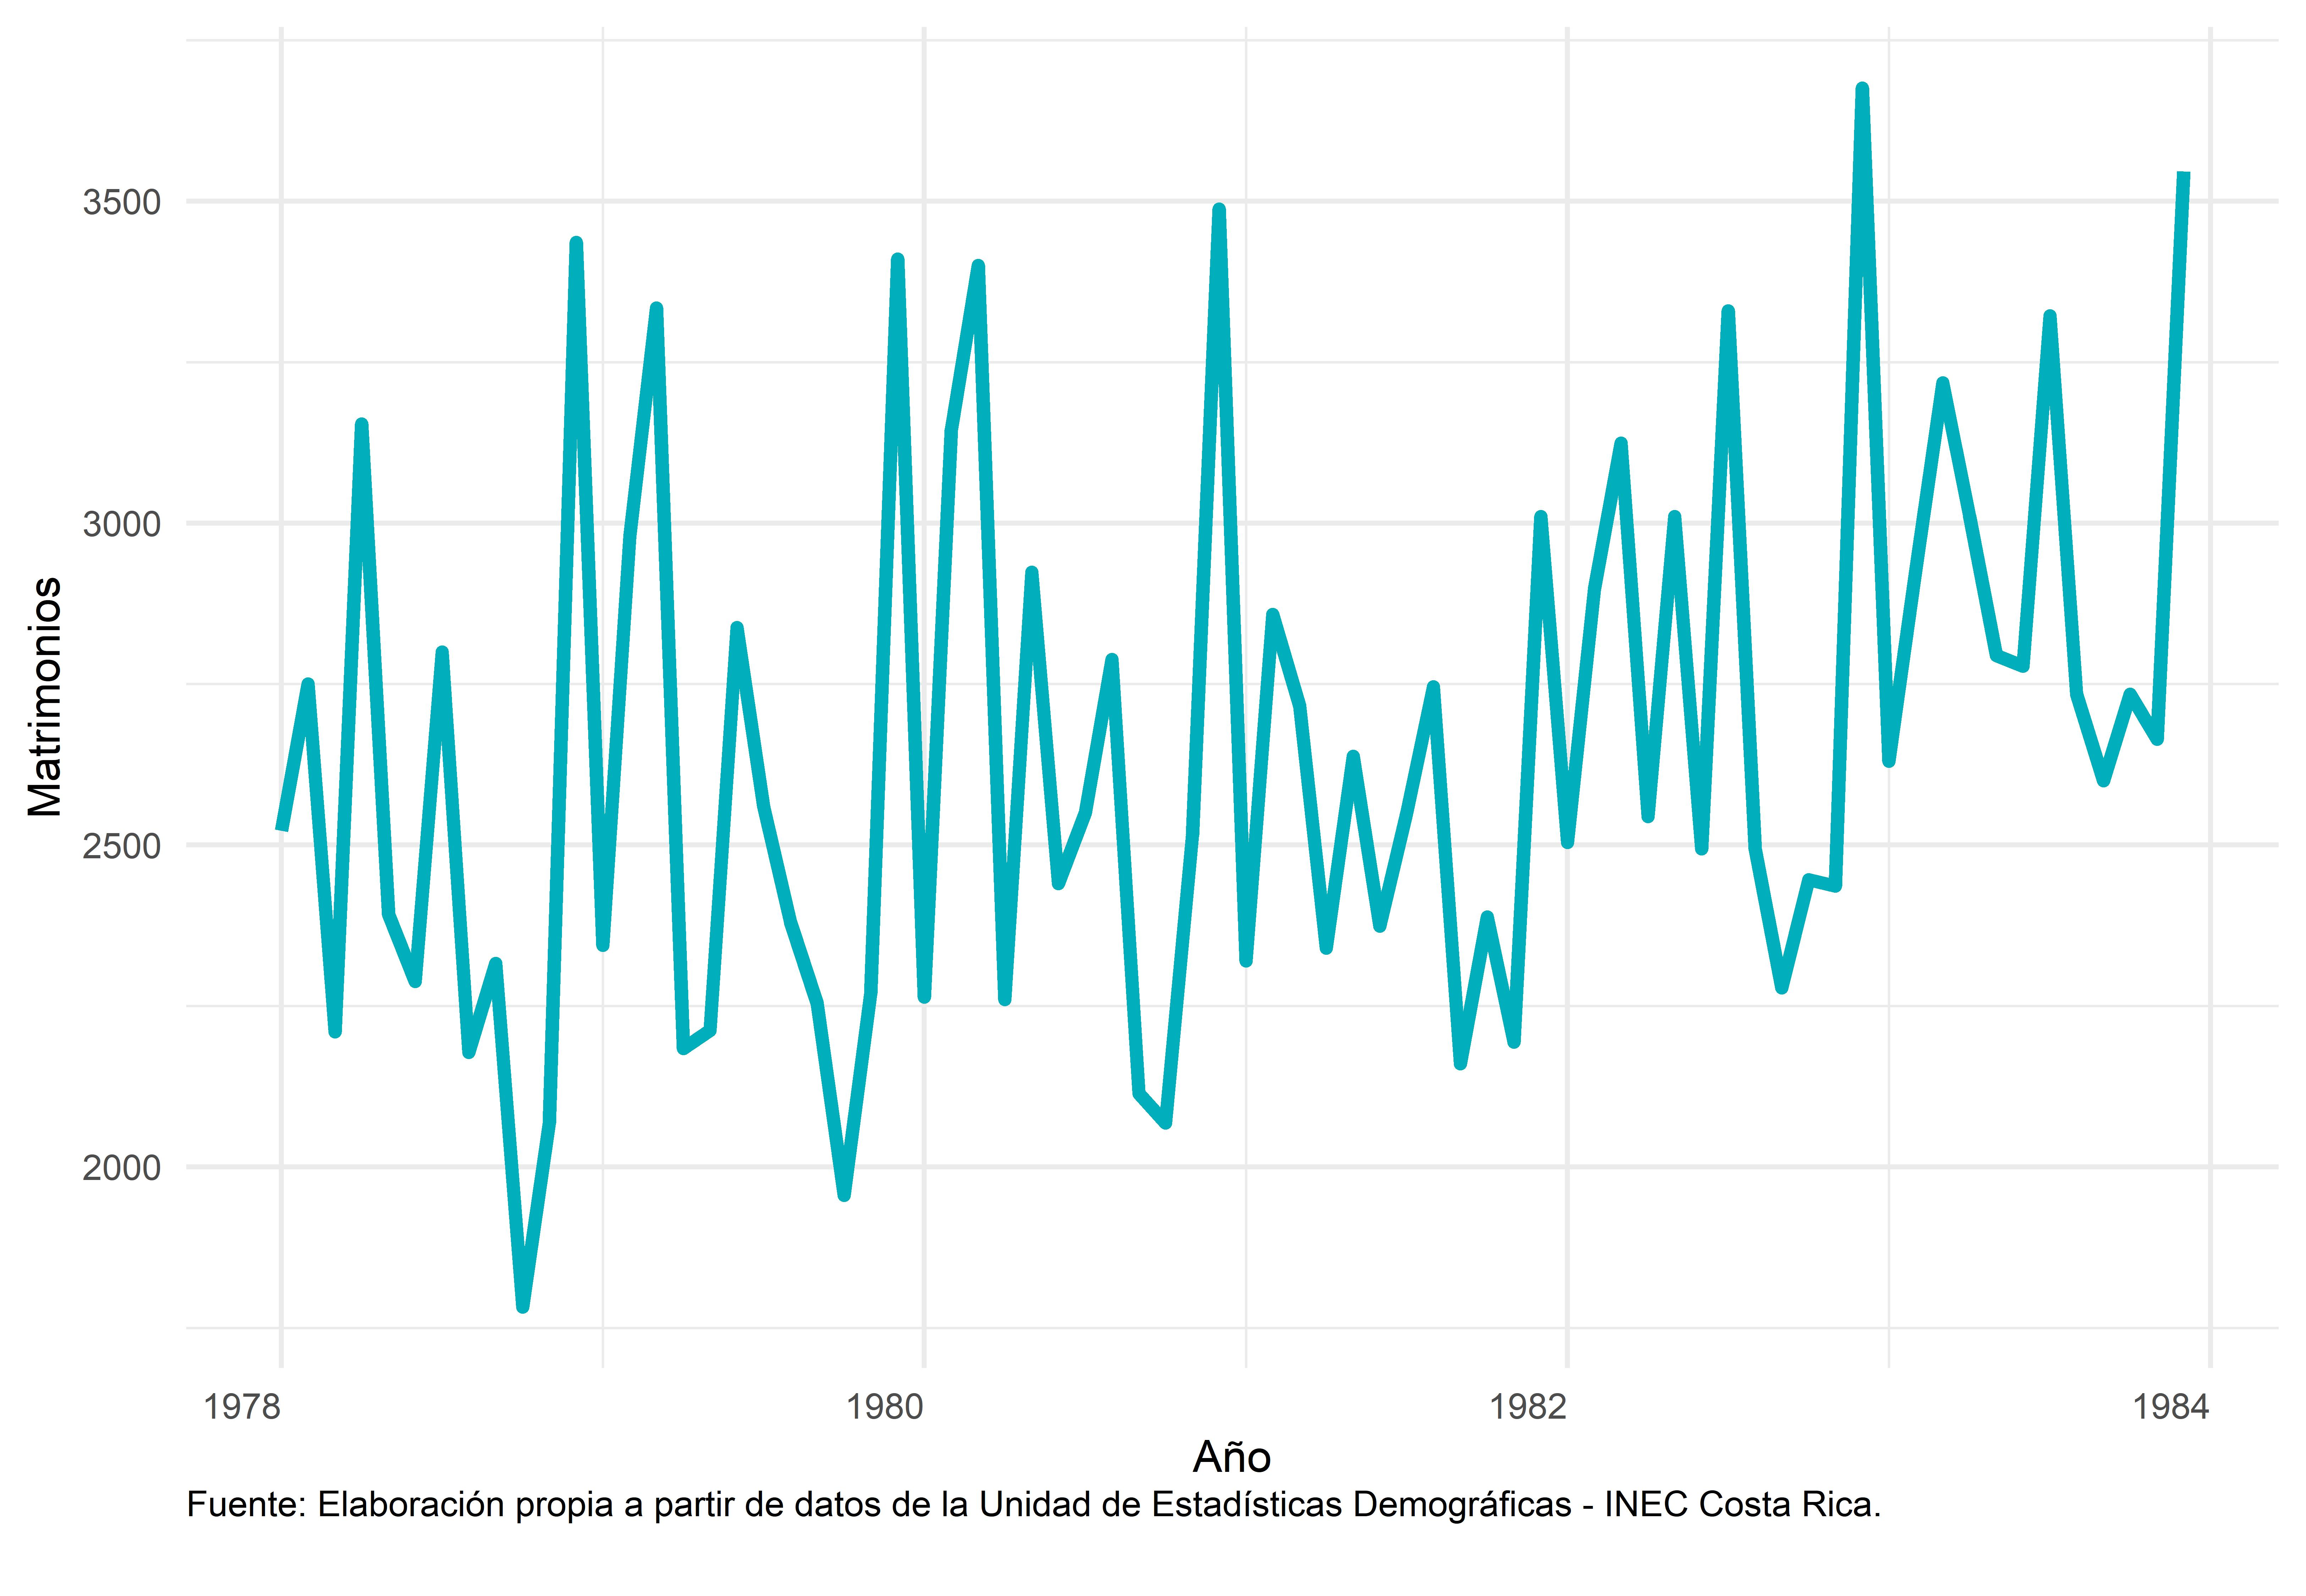
\includegraphics[width=1\linewidth,height=1\textheight]{Tesis_files/figure-latex/ejemplo_aditiva-1} \caption{Número de matrimonios en Costa Rica para el periodo 1978-1983}\label{fig:ejemplo_aditiva}
\end{figure}

\begin{figure}[H]
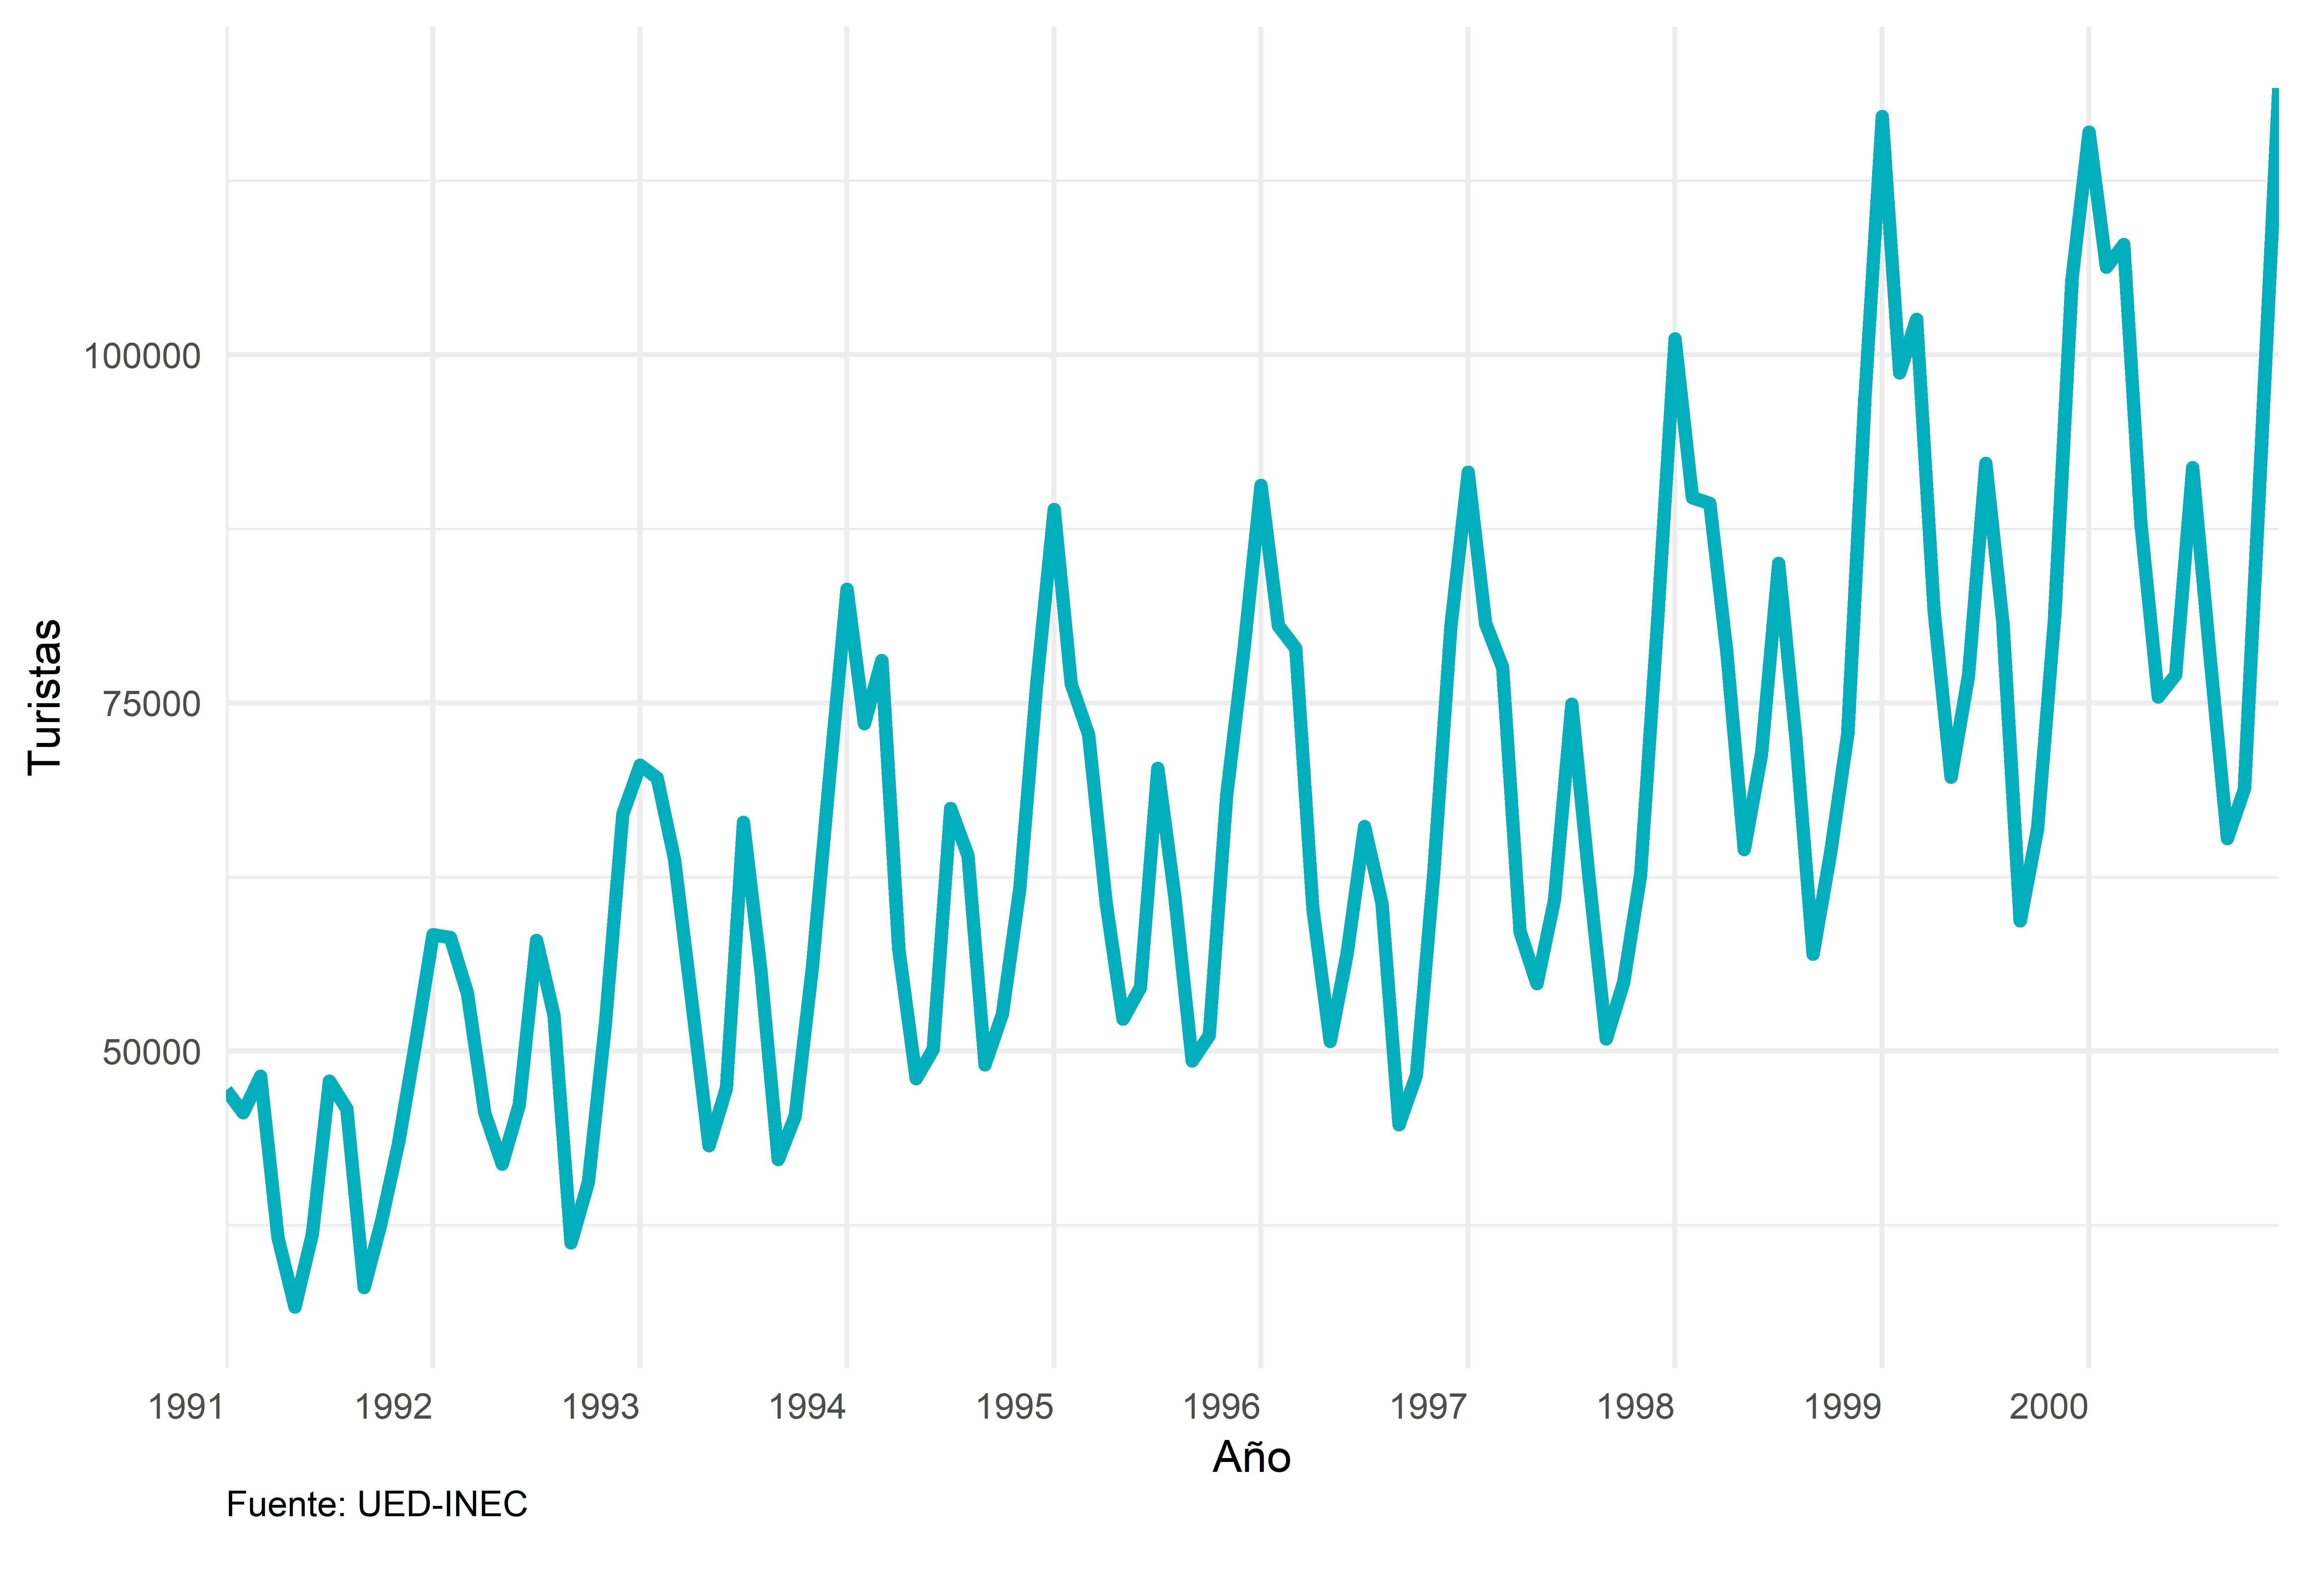
\includegraphics[width=1\linewidth,height=1\textheight]{Tesis_files/figure-latex/ejemplo_multiplicativa-1} \caption{Número de turistas en Costa Rica para el periodo 1991-2000}\label{fig:ejemplo_multiplicativa}
\end{figure}

\subsubsection{La tendencia-ciclo}

A partir del texto de
\protect\hyperlink{ref-calderon2012estadistica}{Calderón}
(\protect\hyperlink{ref-calderon2012estadistica}{2012}), la tendencia
general de una serie cronológica se refiere al crecimiento,
decrecimiento o lateralización de sus movimientos a lo largo del periodo
de estudio. La descomposición clásica de la tendencia-ciclo de este
componente se mantiene constante de un periodo al siguiente. De esta
manera la forma matemática de la tendencia-ciclo para una serie
cronológica se muestra en la ecuación
\ref{eqn:descomposicion_tendencia}.

\begin{equation}
\label{eqn:descomposicion_tendencia}
T(t)=
\begin{cases}
2\bar y_{t,m} & \text{si}\ \text{m es par} \\
\bar y_{t, m} & \text{si}\ \text{m es impar} \\
\end{cases}
\end{equation}

Donde \(\bar y_{t,m}\) representa el promedio móvil de orden \(m\)
alrededor del momento \(t\), que es un promedio de \(m\) observaciones
consecutivas de la serie de tiempo \(y_t\). En el caso de una media
móvil de 12 periodos su cálculo está dado por
\(\bar{y}_{t, 12}=\frac{y_{t-6}+\cdots+y_{t-1}+y_t+y_{t+1}+\cdots+y_{t+5}}{12}\),
con \(t=7,\cdots,n-5\), siendo \(n\) el total de observaciones de la
serie cronológica. Un ejemplo es la serie cronológica del número de
matrimonios en Costa Rica para el periodo 1978-1983, que con el tiempo
su crecimiento suele comportarse de una forma creciente tal y como
muestra la Figura \ref{fig:ejemplo_tendencia}.

\begin{figure}[H]
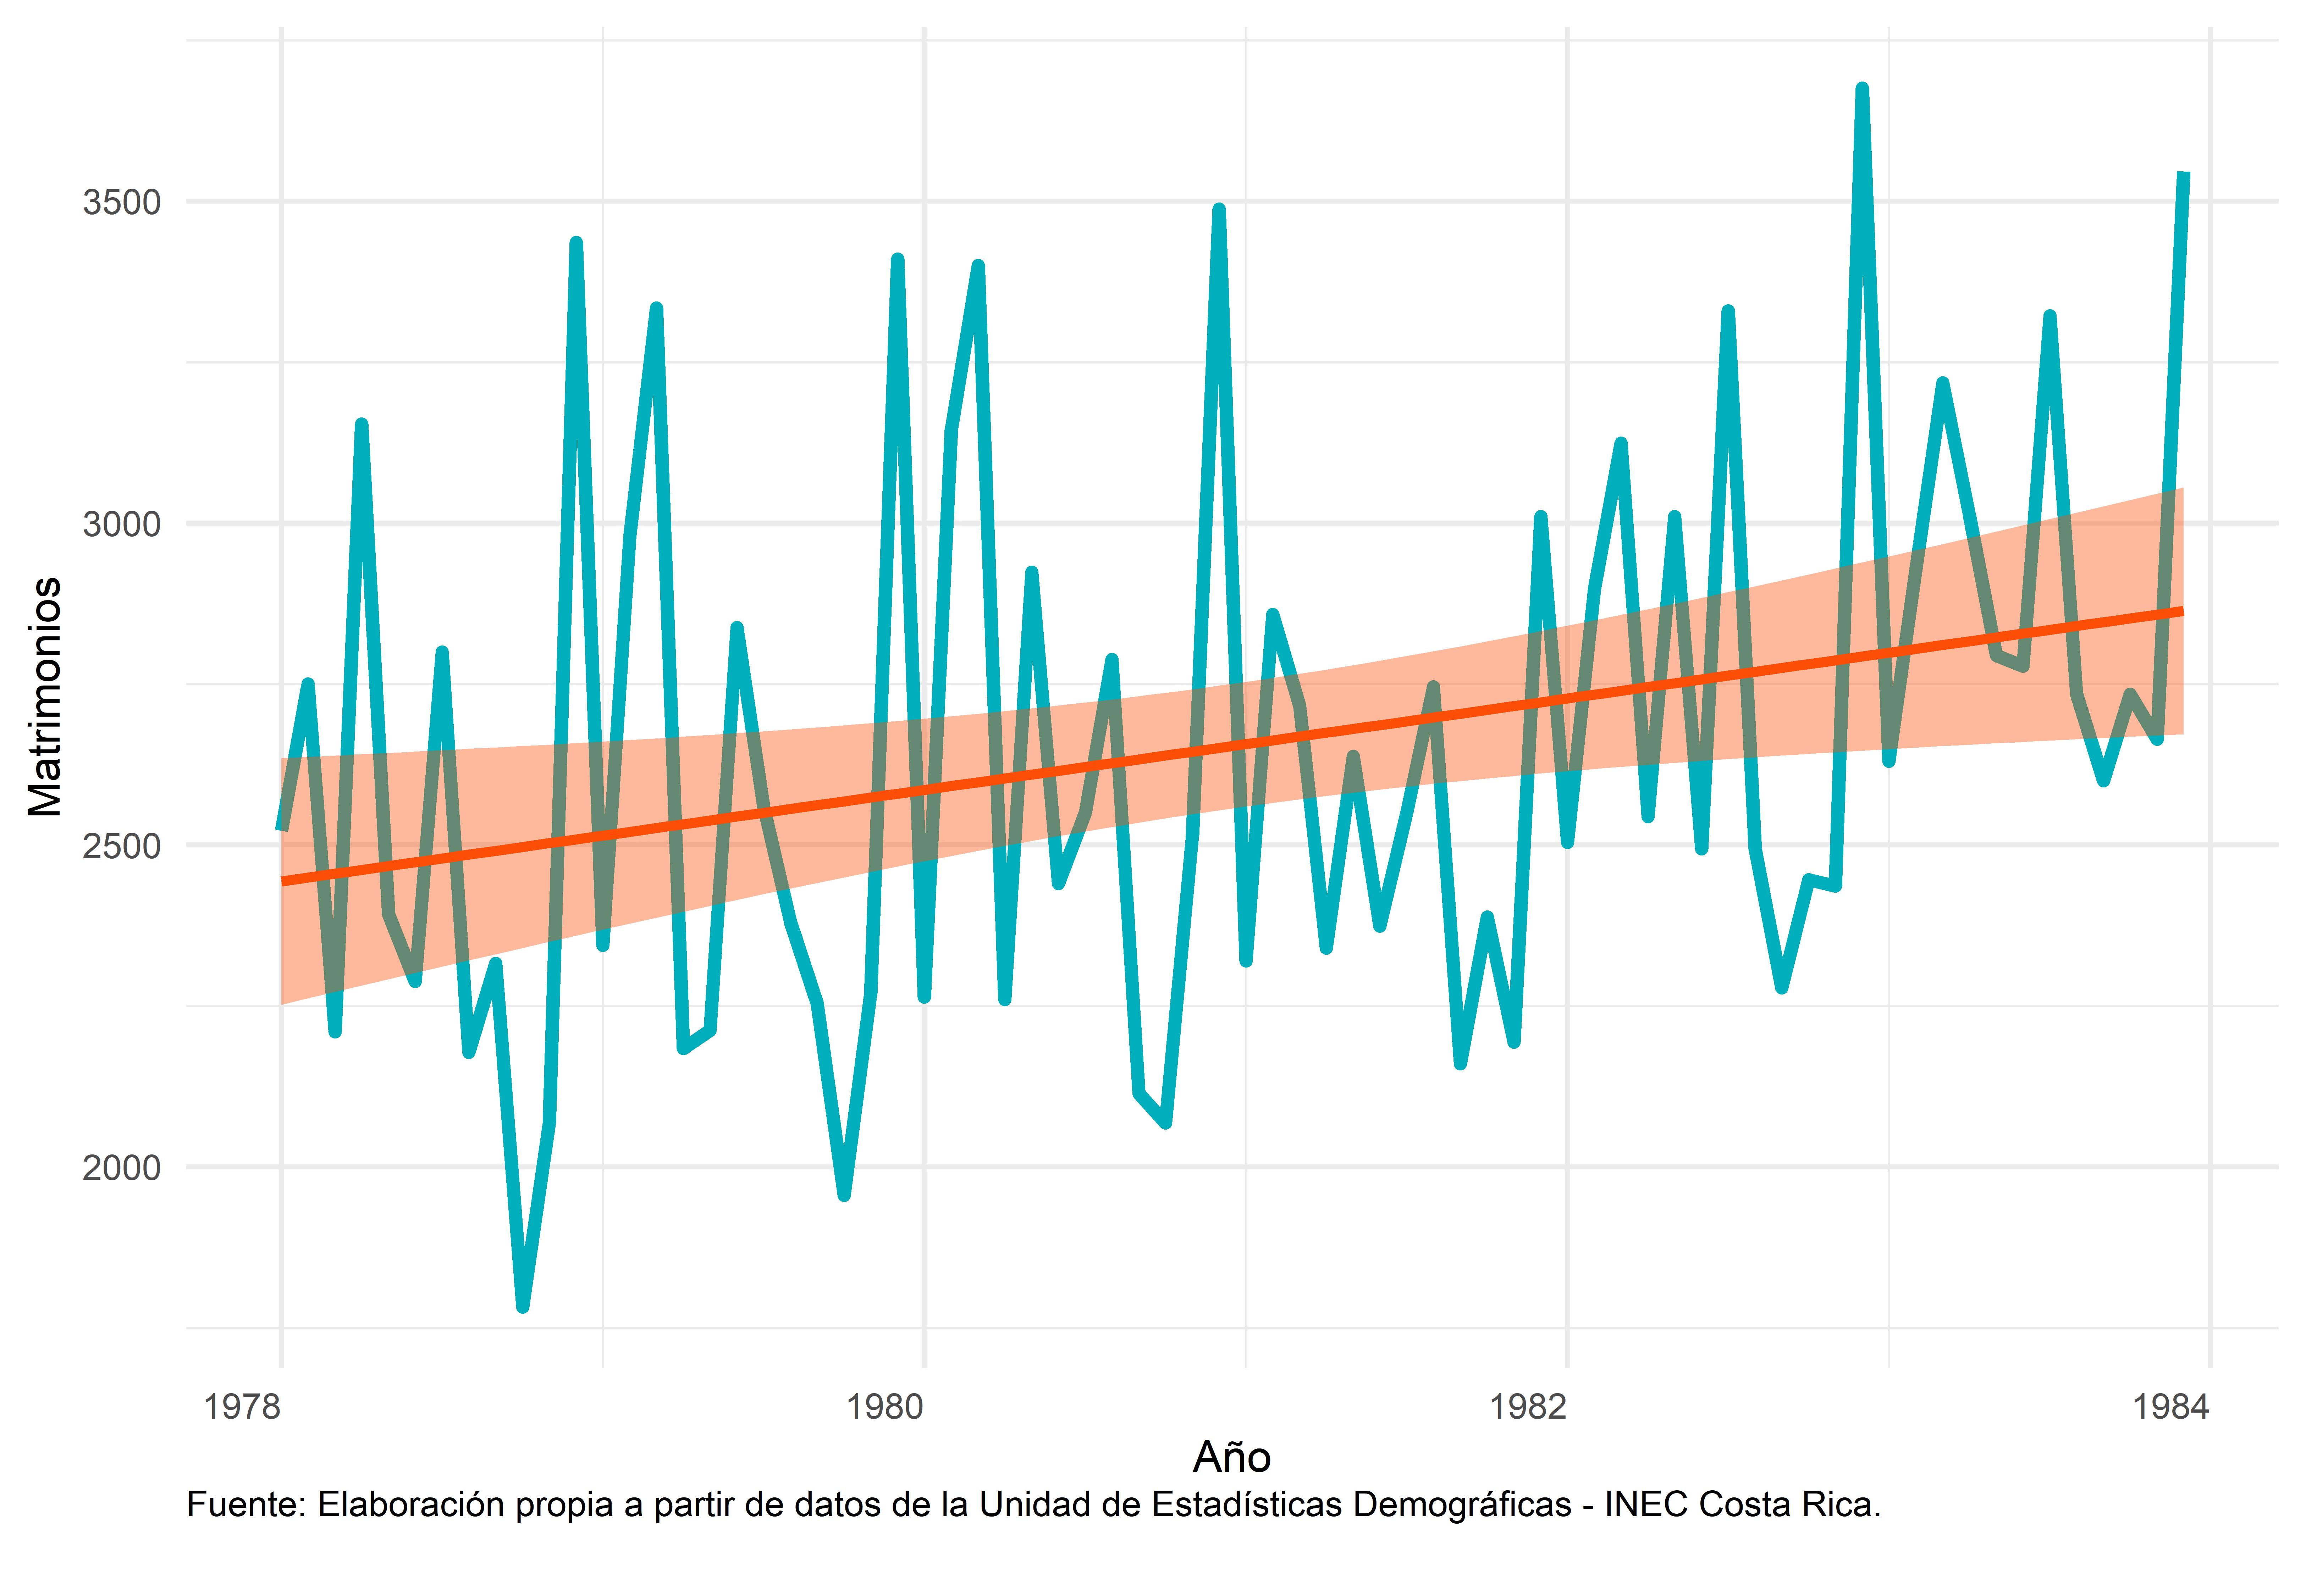
\includegraphics[width=1\linewidth,height=1\textheight]{Tesis_files/figure-latex/ejemplo_tendencia-1} \caption{Tendencia del número de matrimonios en Costa Rica para el periodo 1978-1983}\label{fig:ejemplo_tendencia}
\end{figure}

Del informe elaborado también por
\protect\hyperlink{ref-calderon2012estadistica}{Calderón}
(\protect\hyperlink{ref-calderon2012estadistica}{2012}) se desprende que
los periodos cíclicos, por su parte, se refieren a los cambios que se
dan en una serie cronológica en el mediano-largo plazo, que son causados
por determinados eventos que suelen repetirse. Estos ciclos suelen tener
una duración determinada, como es el caso de los índice bursátil
NASDAQ-100. Este indicador resume el estado de los 100 valores de las
compañías más importantes del sector de la industria de la tecnología, y
sus ciclos suelen presentar un auge, seguido por un descenso que,
posteriormente, se vuelve una depresión, y que finalmente se convierte
en una recuperación a su estado inicial. La Figura
\ref{fig:ejemplo_ciclo} muestra como el índice NASDAQ-100 inicia un auge
alrededor de enero de 1995 (primera línea azul punteada), para luego
experimentar una fuerte caída a partir de junio del año 2000 (línea roja
punteada) y posteriormente iniciar un periodo de recuperación en enero
del año 2009 (segunda línea azul punteada).

\begin{figure}[H]
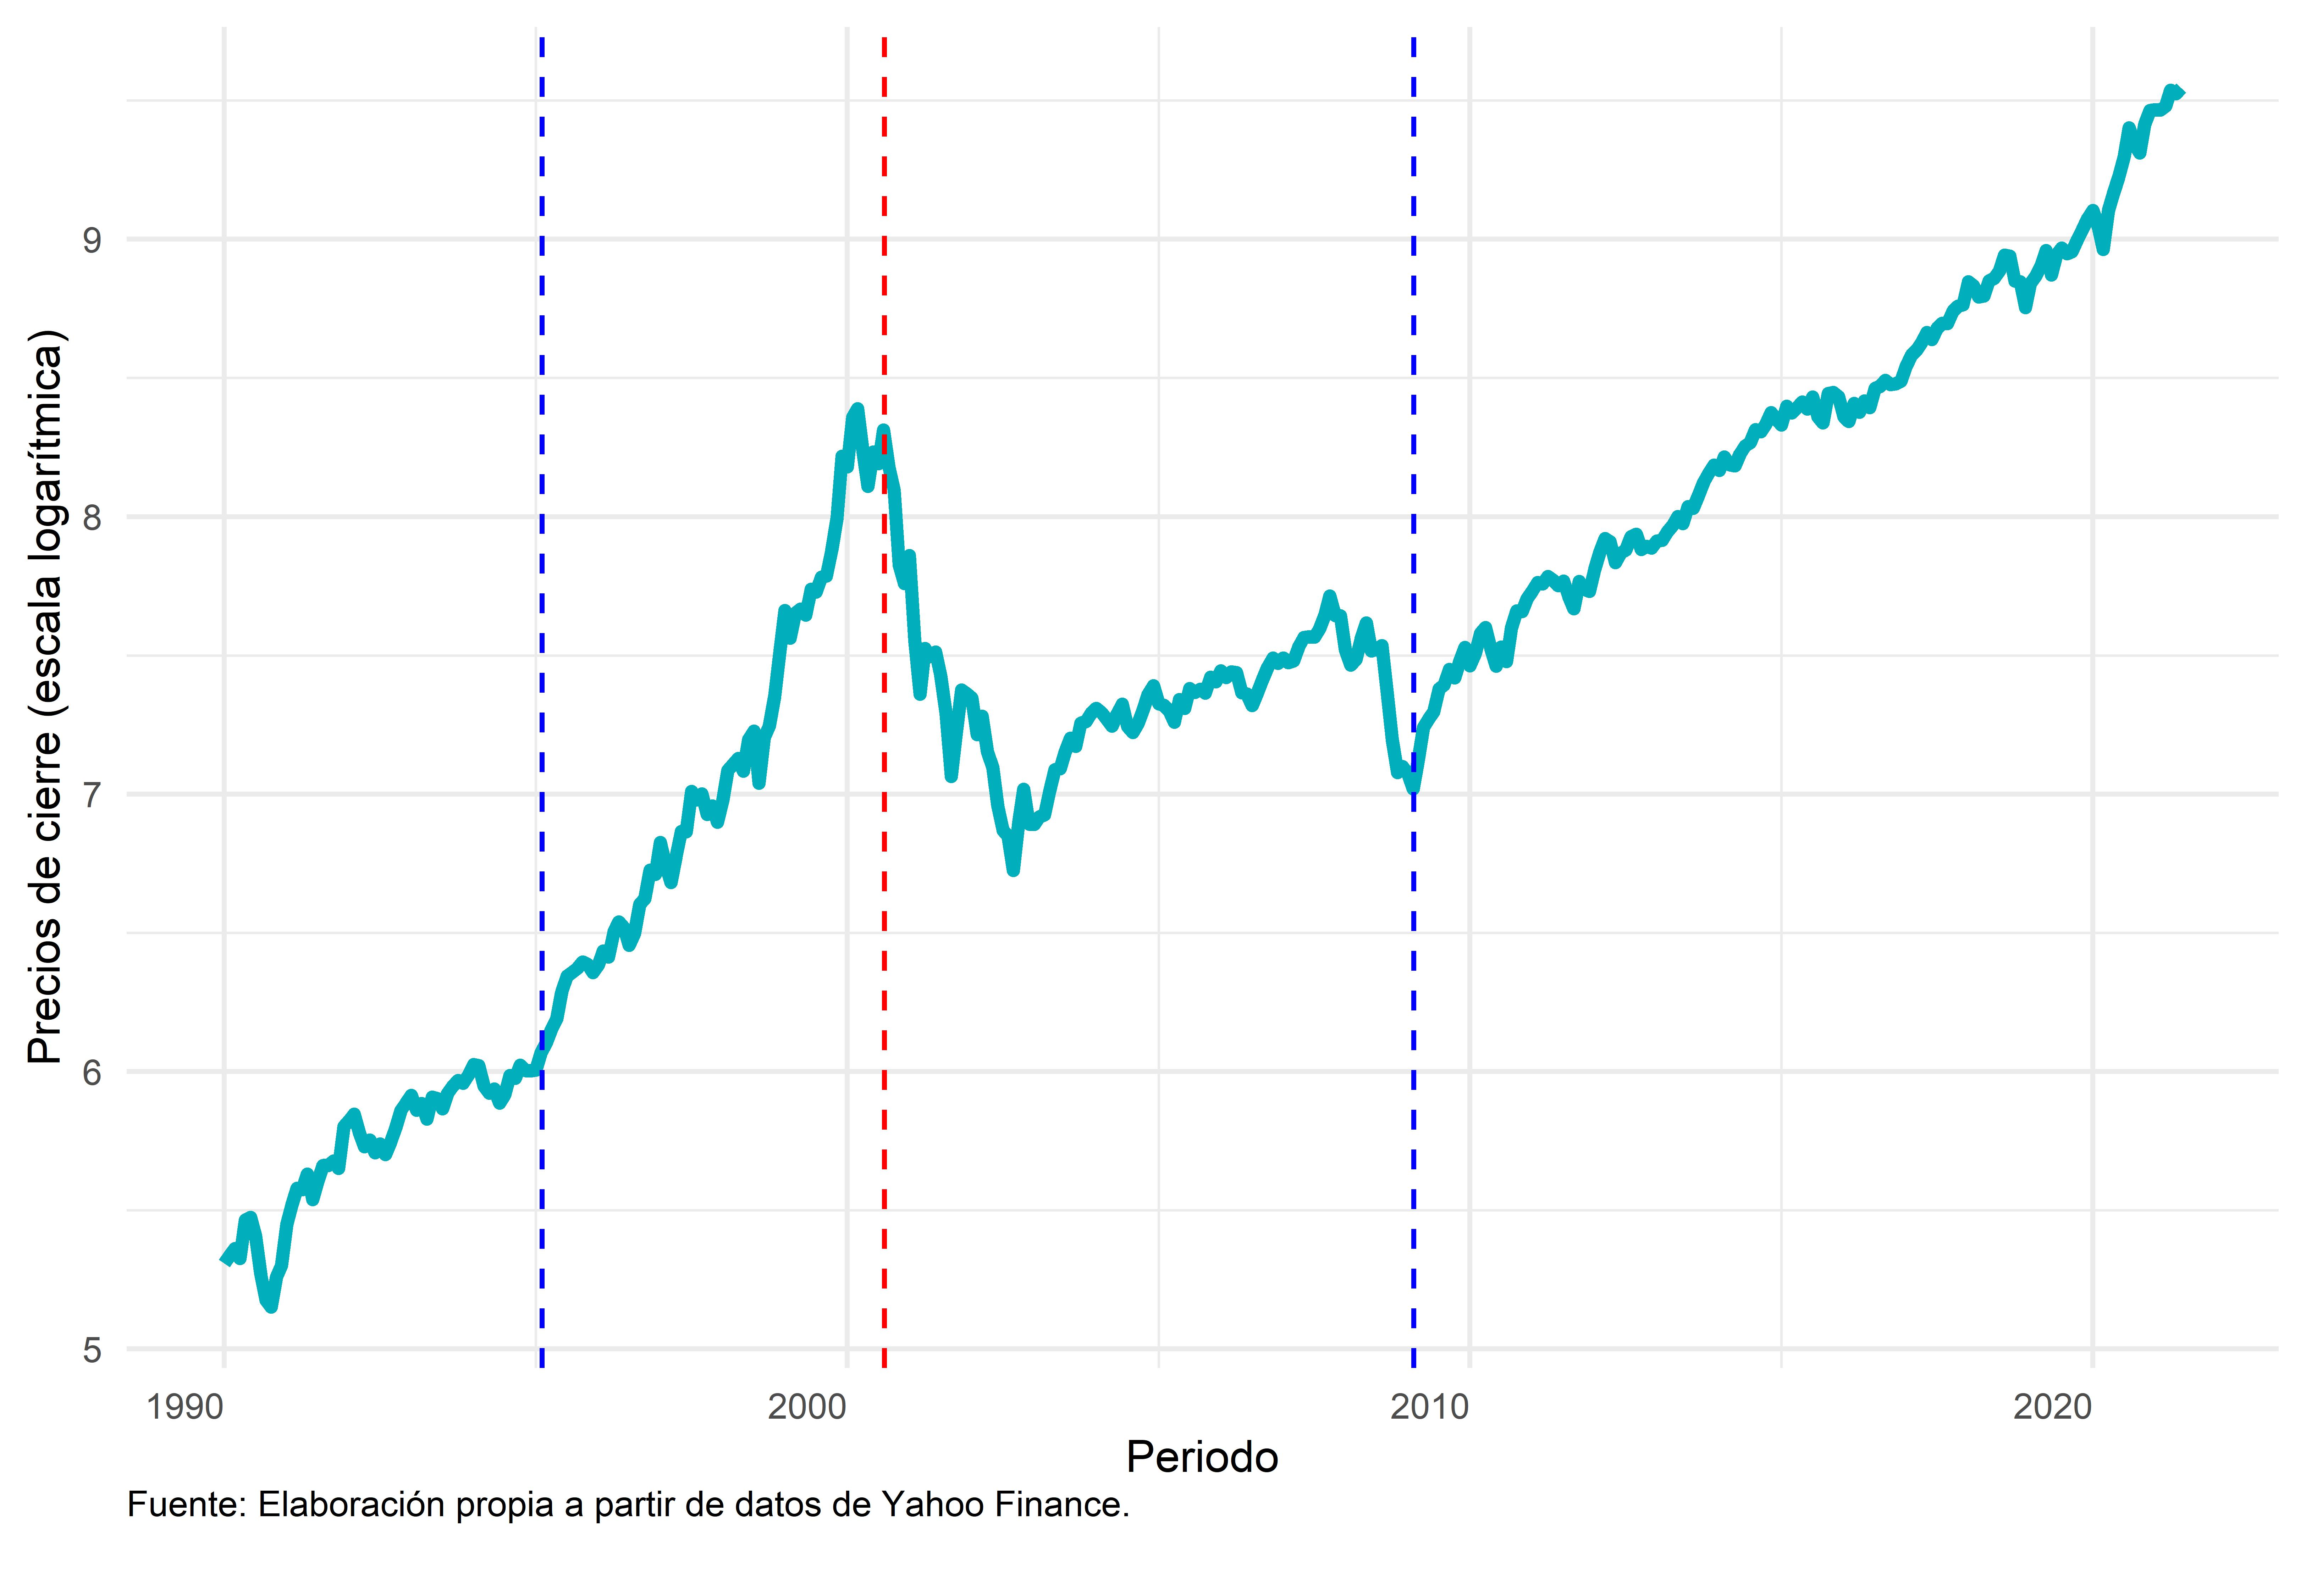
\includegraphics[width=1\linewidth,height=1\textheight]{Tesis_files/figure-latex/ejemplo_ciclo-1} \caption{Índice bursatil NASDAQ-100 para el periodo enero 1990 - junio 2021}\label{fig:ejemplo_ciclo}
\end{figure}

\subsubsection{Componentes estacionales}

\protect\hyperlink{ref-calderon2012estadistica}{Calderón}
(\protect\hyperlink{ref-calderon2012estadistica}{2012}) también se
refiere a los cambios estacionales que se presentan en una serie de
tiempo, los cuales se relacionan con las fluctuaciones naturales del
fenómeno dentro de una temporada de observaciones. Visualmente los
efectos estacionales puede apreciarse en la Figura
\ref{fig:ejemplo_multiplicativa}, en donde los picos más altos de
turistas siempre se ubican entres los meses de diciembre y enero.
Matemáticamente, el componente estacional puede calcularse utilizando la
descomposición clásica como se indica en la ecuación
\ref{eqn:descomposicion_estacional}:

\begin{equation}
\label{eqn:descomposicion_estacional}
S(t)=\psi_{t,a}-\psi^*
\begin{cases}
\psi_{t,a} = \frac{\sum_{i=0}^a \hat{y}_{t+a\cdot i}}{a} \\
\psi^*=\frac{\sum_{i=0}^n \hat{y}_{t+i}}{n} \\
\hat{y}_t=y_t-\bar{y}_{t,S,m} \\
\bar{y}_{t,S,m}=\frac{\sum_{i=1}^m \bar{y}_{t+i-m,S}}{m} \\
\bar{y}_{t,S}=\frac{\sum_{i=1}^S y_{t-i+\frac{S}{2}}}{S} \\
\end{cases}
\end{equation}

donde \(S\) representa la frecuencia estacional (por ejemplo cada 12
meses), \(a\) es la cantidad de periodos estacionales disponibles (por
ejemplo, si se tienen 6 periodos completos de 12 meses, se tienen 6
años), \(m\) es la cantidad de periodos que se utiliza para centrar las
medias móviles, \(y_t\) es la observación de la serie cronológica \(y\)
en el momento \(t\), \(\bar{y}_{t,S}\) es el promedio móvil de \(S\)
periodos alrededor del momento \(t\) de las serie \(y_t\),
\(\bar{y}_{t,S,m}\) es el promedio móvil centrado de en \(m\) periodos
de la serie \(y_t\), \(\hat{y}_t\) es la serie de tiempo \(y_t\) sin el
efecto de la tendencia-ciclo, \(\psi^*\) es el promedio de los valores
obtenidos para \(\hat{y}_t\), y \(\psi_{t,a}\) es el promedio de los
\(a\) periodos estacionales sin el efecto de la tendencia-ciclo.
Gráficamente, el componente estacional se muestra en la Figura
\ref{fig:ejemplo_estacional}.

\begin{figure}[H]
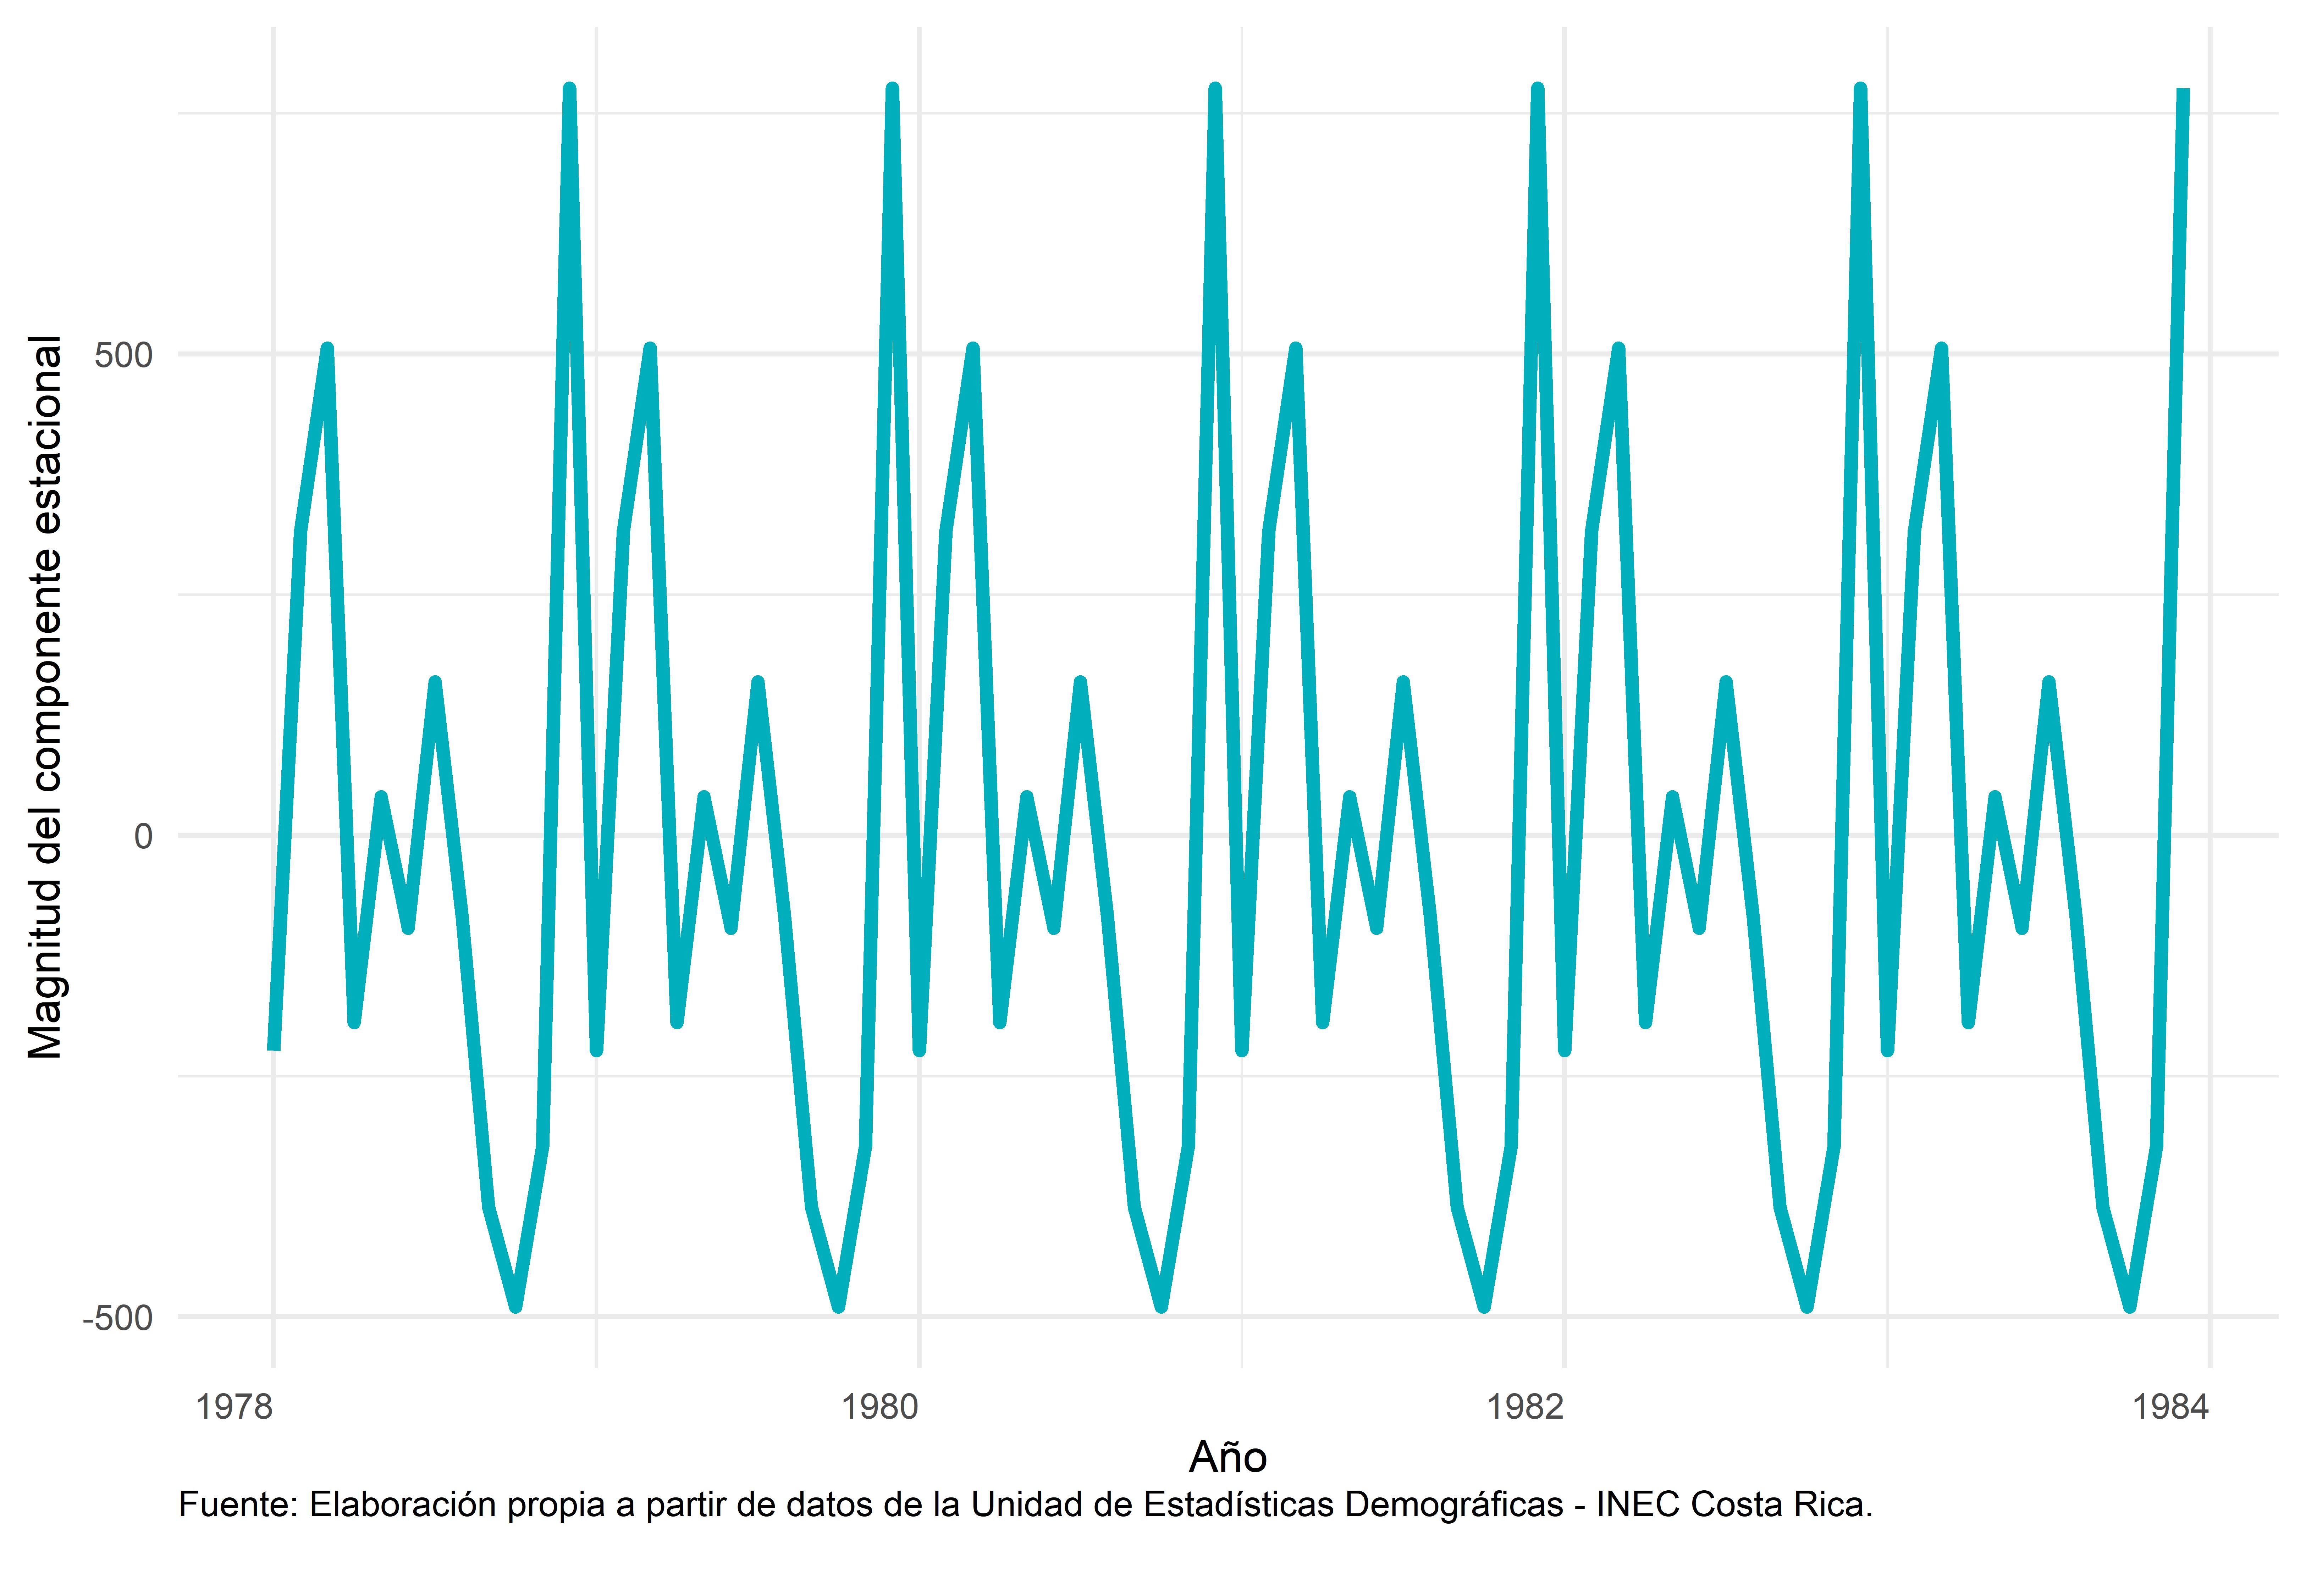
\includegraphics[width=1\linewidth,height=1\textheight]{Tesis_files/figure-latex/ejemplo_estacional-1} \caption{Componente aleatorio de la serie de matrimonios en Costa Rica para el periodo 1978-1983}\label{fig:ejemplo_estacional}
\end{figure}

\subsubsection{Componente irregular}

Finalmente, la irregularidad de una serie cronológica, siguiendo a
\protect\hyperlink{ref-calderon2012estadistica}{Calderón}
(\protect\hyperlink{ref-calderon2012estadistica}{2012}), se refiere a
las fluctuaciones propias de un fenómeno que no pueden ser predichas.
Estos cambios no se dan de manera regular, es decir, no siguen un patrón
determinado. Matemáticamente su descomposición se obtiene a partir de
los otros componentes así como de la propia serie cronológica \(y(t)\),
tal y como se muestra en la ecuación \ref{eqn:descomposicion_irregular}.
Visualmente, la magnitud del componente aleatorio se muestra en la
Figura \ref{fig:ejemplo_aleatorio}

\begin{equation}
\label{eqn:descomposicion_irregular}
I(t)=
\begin{cases}
y(t)-T(t)-S(t), & \text{si}\ \text{la serie es aditiva} \\
\frac{y(t)}{T(t)S(t)} , & \text{si}\ \text{la serie es multiplicativa} \\
\end{cases}
\end{equation}

\begin{figure}[H]
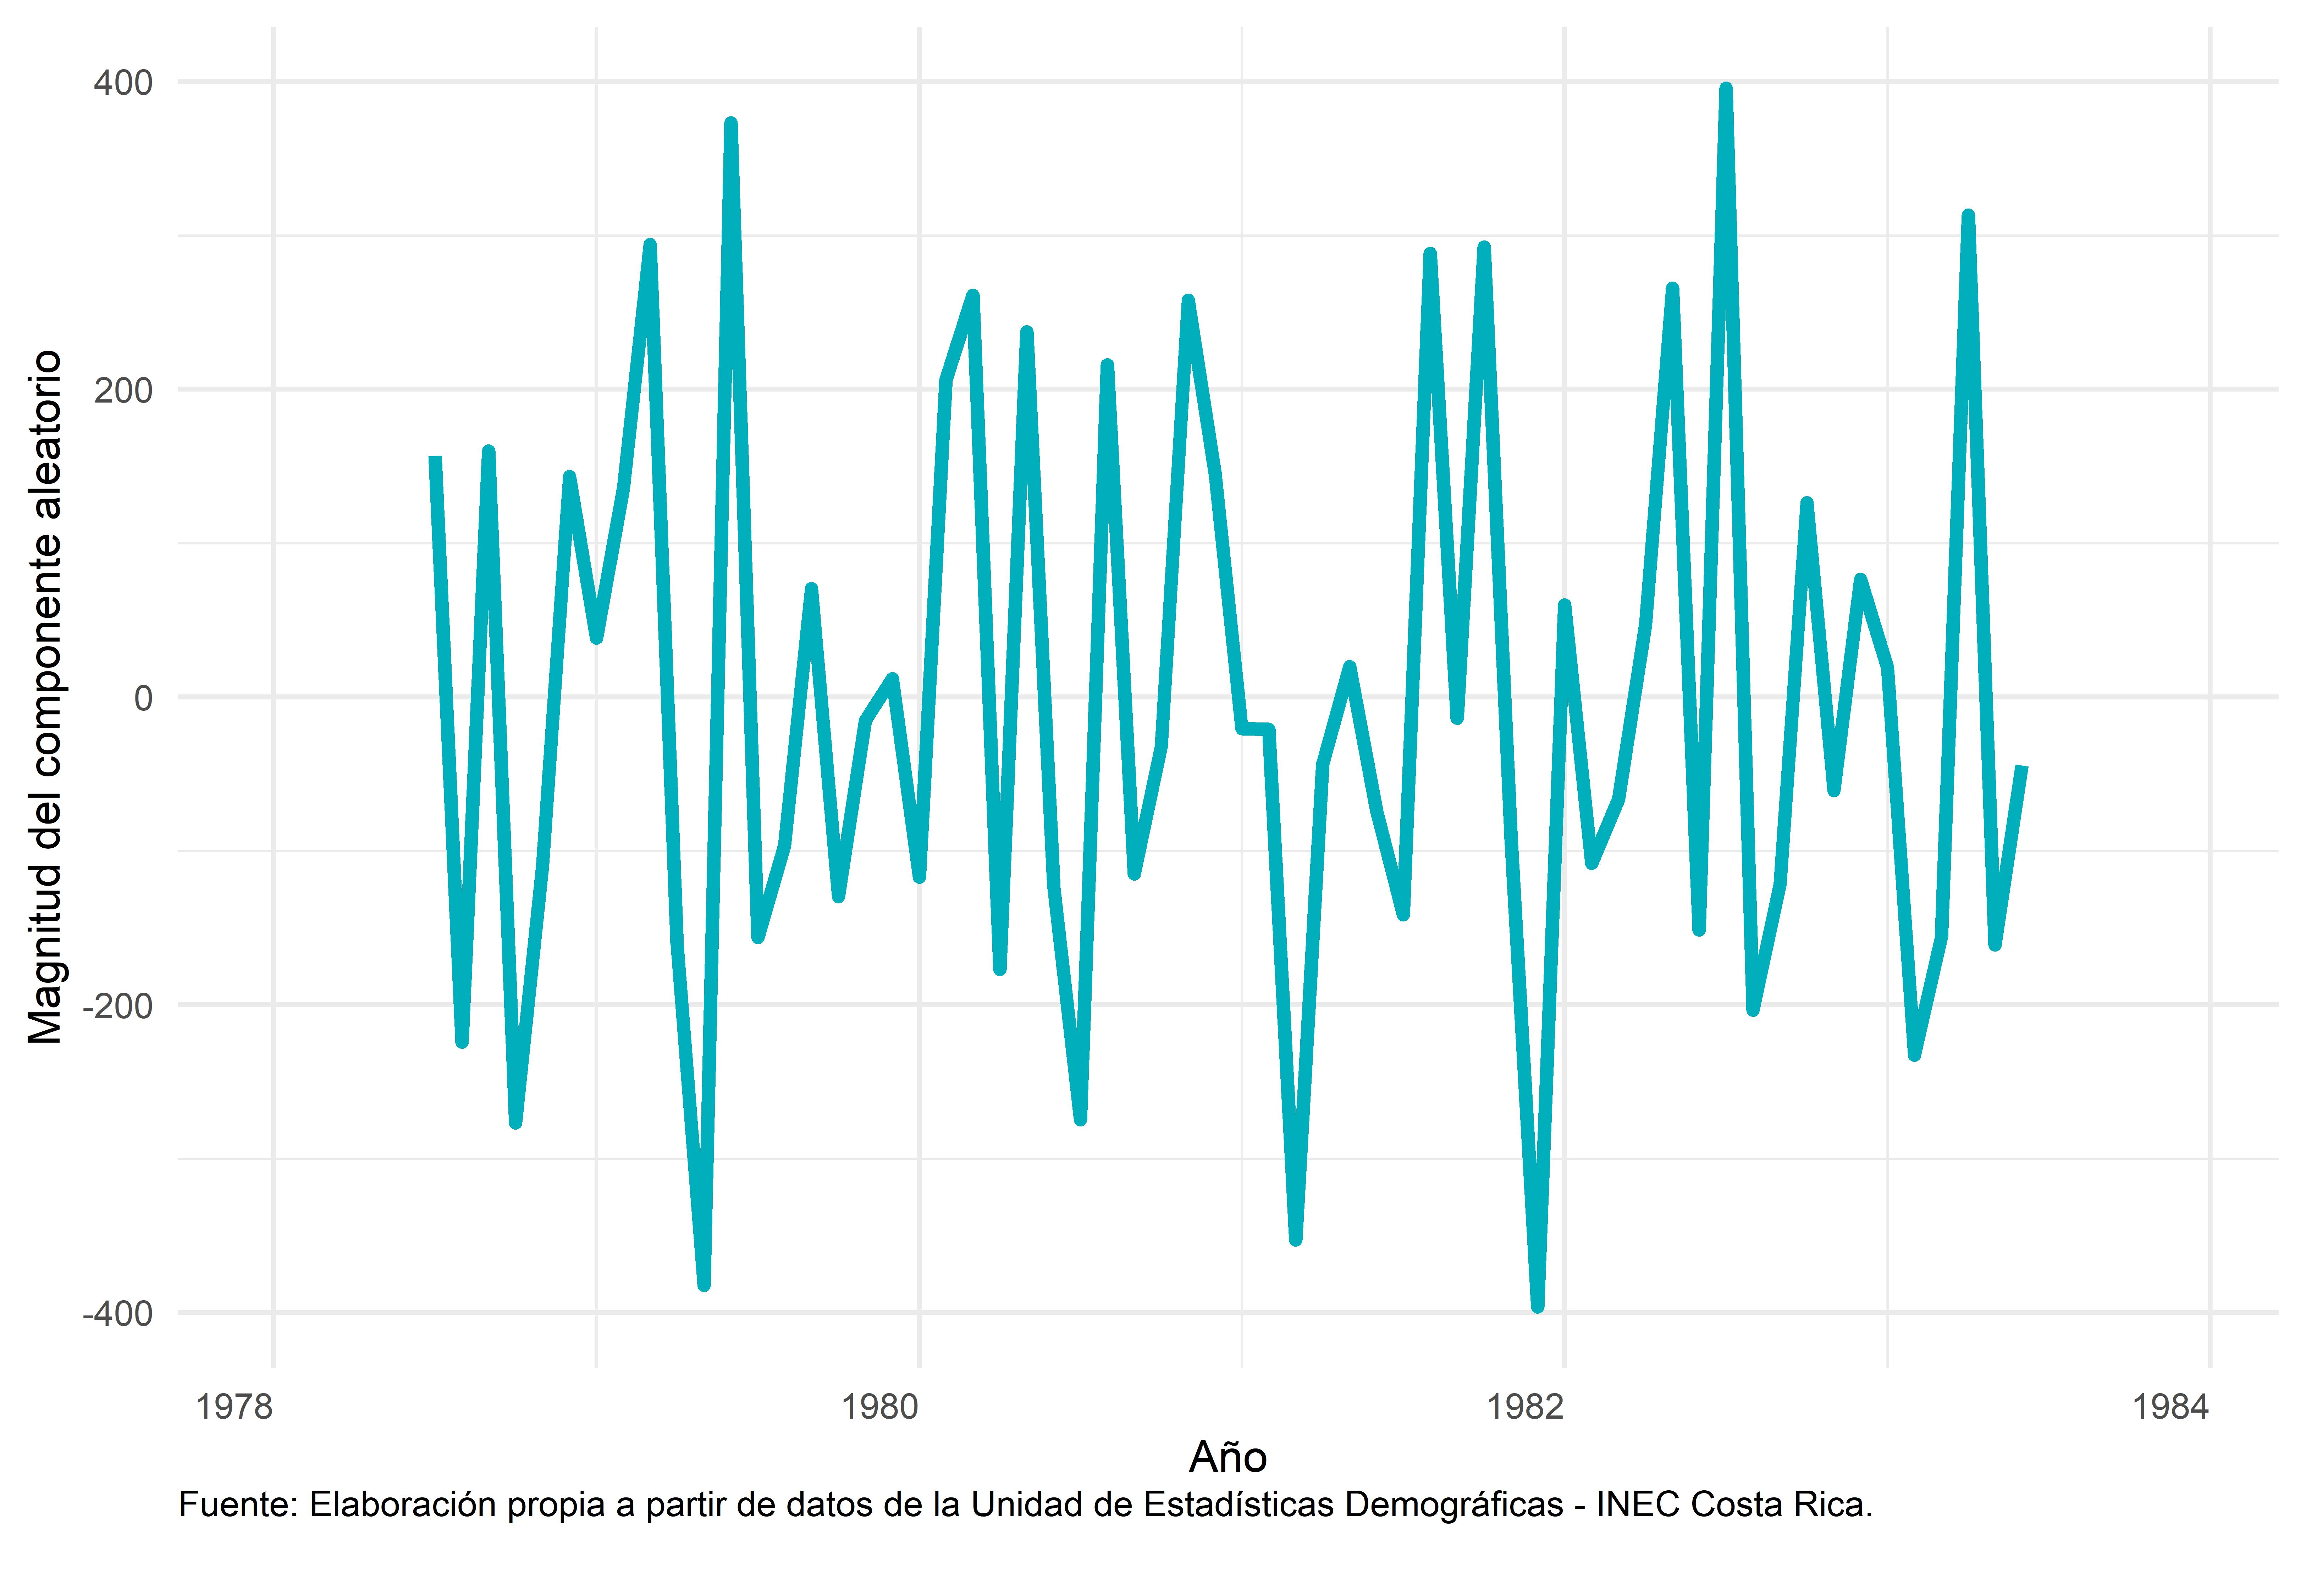
\includegraphics[width=1\linewidth,height=1\textheight]{Tesis_files/figure-latex/ejemplo_aleatorio-1} \caption{Componente aleatorio de la serie de matrimonios en Costa Rica para el periodo 1978-1983}\label{fig:ejemplo_aleatorio}
\end{figure}

\subsection{Supuestos en el análisis de series cronológicas}

El análisis de series temporales, según
\protect\hyperlink{ref-Hipel}{Hipel \& McLeod}
(\protect\hyperlink{ref-Hipel}{1994}), representa un método para
comprender la naturaleza de la serie en cuestión y poder utilizarla para
generar pronósticos. Es en este sentido que entran en escena las
observaciones recolectadas de la serie, pues ellas son analizadas y
sujetas a modelados matemáticos que logren capturar el proceso que
gobierna a toda la serie cronológica
(\protect\hyperlink{ref-Zhang}{Zhang, 2003}).

En un proceso determinístico, es posible predecir con certeza lo que
ocurrirá en el futuro pues carecen de aleatoriedad, razón por la cual el
proceso definirse fácilmente mediante una ecuación matemática; las
series cronológicas, sin embargo, carecen de esta condición. Por el
contrario, los procesos no determinísticos son aquellos que no pueden
describirse con exactitud mediante una ecuación matemática, sino que
deben aproximarse debido al componente aleatorio que poseen de forma
intrínseca. Una serie de tiempo puede tratarse de un proceso no
determinístico porque usualmente, toda la información que se necesita
para describir el proceso de manera determinística es desconocida, o
bien porque la naturaleza de la información involucra la aleatoriedad,
de esta manera, como los procesos no determinísticos consideran un
aspecto aleatorio, pueden estimarse mediante leyes probabilísticas.
\protect\hyperlink{ref-Hipel}{Hipel \& McLeod}
(\protect\hyperlink{ref-Hipel}{1994}) sugieren que una serie cronológica
puede considerarse como una muestra aleatoria de una serie mucho más
grande, es decir, una serie cronológica puede verse como una colección
de variables aleatorias ordenadas de manera cronológica. La magnitud de
estas variaciones aleatorias pueden variar en función del tiempo, esta
condición se conoce como un proceso estocástico (aleatorio)
(\protect\hyperlink{ref-definicion_estocastico}{Elmabrouk, n.d.}).

De acuerdo con \protect\hyperlink{ref-stationary_def}{Agrawal \&
Adhikari} (\protect\hyperlink{ref-stationary_def}{2013}), una serie se
considera estacionaria cuando su nivel medio y su variancia son
aproximadamente las mismas durante todo el periodo, es decir, el tiempo
no afecta a estos estadísticos de variabilidad. A partir del texto de
\protect\hyperlink{ref-introduccion_series}{Ramírez}
(\protect\hyperlink{ref-introduccion_series}{2007}), una forma de
definir un proceso débilmente estacionario o estacionario de segundo
orden \(Y_t\) es mediante los momentos poblacionales de primer y segundo
orden tal y como se define en la ecuación
\ref{eqn:ecuacion_estocastico}.

\begin{equation}
\label{eqn:ecuacion_estocastico}
Y_t:
\begin{cases}
E(Y_t) = \mu_t, \forall t \\
V(Y_t) = \sigma^2_t, \forall t \\
COV(T_t,Y_s) = E\left[(Y_t-\mu_t)(Y_s-\mu_s)\right], \forall t,s \\
\end{cases}
\end{equation}

El supuesto de estacionariedad busca simplificar la identificación del
proceso con el objetivo de obtener un modelo adecuado para generar los
pronósticos. De acuerdo con
(\protect\hyperlink{ref-definicion_estocastico}{Elmabrouk, n.d.}), se
dice que una serie cronológica \(Y_t\) es fuertemente estacionaria
cuando la distribución de probabilidad de dicho proceso en cualquier
momento \(t\) es aproximadamente la misma para cualquier momento en el
tiempo, mientras que es débilmente estacionaria si su media y su función
de correlación no varía en el tiempo. Si una serie cronológica posee
tendencias o patrones estacionales hace que esta sea no estacionaria. En
la práctica, una serie puede volverse estacionaria al aplicarle
transformaciones o diferenciaciones de distinto orden.

Como una serie temporal es una observación o una realización de un
proceso estocástico, éstas se encuentran sujetas a múltiples supuestos.
En los modelos lineales definidos como procesos estocásticos uno de
ellos es que todas las observaciones son independientes e idénticamente
distribuidas (i.i.d.), que según
\protect\hyperlink{ref-definicion_iid}{Evans \& Rosenthal}
(\protect\hyperlink{ref-definicion_iid}{2005}), un conjunto de variables
aleatorias \(Y_1,...,Y_n\) son independientes e idénticamente
distribuidas si el conjunto es independiente y además cada una de las n
variables sigue la misma distribución, que usualmente se define como una
distribución aproximadamente Normal, con una media y variancia dadas;
esta condición es deseable, sin embargo, en un modelo de series de
tiempo un proceso estocástico puede no ser independiente al tener una
estructura que genere un patrón reiterado en el tiempo. Este supuesto
puede dividirse según el tipo de variable aleatoria:

\textbf{1.}: Si el conjunto de variables \(Y_1,...,Y_n\) pertenecen a
una distribución discreta, cada función de probabilidad es idéntica, de
manera que \(p_{y_1}(y)=p_{y_2}(y)=\cdots=p_{y_n}(y)\equiv p(y)\), y
además
\(p_{y_1,...,y_n}(y_1,...,y_n)=p_{y_1}(y_1)p_{y_2}(y_2)\cdots p_{y_n}(y_n)=p(y_1)p(y_2)\cdots p(y_n)\).

\textbf{2.}: Si el conjunto de variables \(Y_1,...,Y_n\) pertenecen a
una distribución continua, cada función de probabilidad es idéntica, de
manera que \(f_{y_1}(y)=f_{y_2}(y)=\cdots=f_{y_n}(y)\equiv f(y)\), y
además
\(f_{y_1,...,y_n}(y_1,...,y_n)=f_{y_1}(y_1)f_{y_2}(y_2)\cdots f_{y_n}(y_n)=f(y_1)f(y_2)\cdots f(y_n)\).

Lo anterior es contrario al uso de las observaciones pasadas para
pronosticar el futuro, por lo que este supuesto, según
\protect\hyperlink{ref-Cochrane}{Cochrane}
(\protect\hyperlink{ref-Cochrane}{1997}), no es exacto pues una una
serie de tiempo no es exactamente, i.i.d., sino que siguen un patrón
medianamente regular en el largo plazo. Además, los coeficientes del
proceso que gobierna la serie cronológica, como mencionan
\protect\hyperlink{ref-invertible_estacionario3}{McLeod}
(\protect\hyperlink{ref-invertible_estacionario3}{1999}), son polinomios
que no deben compartir raíces comunes.

Además, existe un principio deseable que es quizá el que más debate
genera, este es el criterio de parsimonia. Como mencionan
\protect\hyperlink{ref-Zhang}{Zhang}
(\protect\hyperlink{ref-Zhang}{2003}) y
\protect\hyperlink{ref-Hipel}{Hipel \& McLeod}
(\protect\hyperlink{ref-Hipel}{1994}), este principio sugiere que se
prioricen modelos sencillos, con pocos parámetros, para representar una
serie de datos. Mientras más grande y complicado sea el modelo, mayor
será el riesgo de sobre ajuste, lo que implica que el ajuste sea muy
bueno en el conjunto de datos con que se generó el modelo, pero que los
pronósticos generados sean pobres ante nuevos conjuntos de datos. Este
problema, sin embargo, se presenta al considerar un único modelo con
muchos parámetros; pero si se consideran varios modelos y estos son
sometidos a distintos criterios, puede obtenerse un modelo
sobreparametrizado que ofrezca buenos pronósticos.

\subsection{Identificación del modelo}

Los métodos más clásicos para la identificación del proceso que gobierna
a una serie cronológica son las funciones de autocorrelación y
autocorrelación parcial, las cuales sirven de indicador acerca de qué
tan relacionadas están las observaciones unas de otras. Estas funciones
ofrecen indicios sobre el orden de los términos para los modelos
\(AR(p)\), \(MA(q)\) y para la diferenciación y, por ende, para la
identificación de un modelo \(ARIMA\)
(\protect\hyperlink{ref-hyndman_box-jenkins}{Hyndman \& Athanasopoulos,
2018b}).

Para medir la relación lineal entre dos variables cuantitativas es común
utilizar el coeficiente de correlación \(r\) de Pearson
(\protect\hyperlink{ref-pearson}{Benesty \& Chen, 2009}), el cual se
define para dos variables \(X\) e \(Y\) como se muestra en la ecuación
\ref{eqn:pearson}.

\begin{equation}
\label{eqn:pearson}
r_{X,Y}=\frac{E(XY)}{\sigma_X \sigma_Y} = \frac{\sum_{i=1}^n \left(X_i- \bar X\right) \left(Y_i- \bar Y\right)}{\sqrt{\sum_{i=1}^n \left(X_i- \bar X\right)^2 \sum_{i=1}^n \left(Y_i- \bar Y\right)^2}}
\end{equation}

Este mismo concepto puede aplicarse a las series cronológicas para
comparar el valor de la misma en el tiempo \(t\), con su valor en el
tiempo \(t-1\), es decir, se comparan las observaciones consecutivas
\(Y_t\) con \(Y_{t-1}\). Esto también es aplicable a no solo una
observación rezagada \((Y_{t-1})\), sino también con múltiples rezagos
\((Y_{t-2}), (Y_{t-3}), \cdots,(Y_{t-n})\). Para esto se hace uso del
coeficiente de autocorrelación.

La función de autocorrelación (\emph{ACF} por sus siglas en inglés)
recibe su nombre debido a que se utiliza el coeficiente de correlación
para pares de observaciones \(r_{Y_t, Y_{t-1}}\) de la serie
cronológica. Al conjunto de todas las autocorrelaciones se le llama
función de autocorrelación.

La función de autocorrelación parcial (\emph{PACF} por sus siglas en
inglés), busca medir la asociación lineal entre las observaciones
\(Y_t\) y \(Y_{t-k}\), es decir, la correlación entres dos observaciones
distintas separadas por \(k\) periodos, descartando los efectos de los
rezagos \(1,2, \cdots ,k-1\); esta correlación puede obtenerse a partir
de la ecuación \ref{eqn:pearson}, que al adaptarse a dos observaciones
de la misma serie cronológica se obtiene el resultado de la ecuación
\ref{eqn:pearson_adaptada_autocorrelacion}.

\begin{equation}
\label{eqn:pearson_adaptada_autocorrelacion}
r_{{Y_t},{Y_{t-k}}}=\frac{E({Y_t}{Y_{t-k}})}{\sigma_{Y_t} \sigma_{Y_{t-k}}} = \frac{\sum_{i=1}^n \left({Y_t}_i- \bar{Y}_t \right) \left({Y_{t-k}}_i- \bar {Y_{t-k}}\right)}{\sqrt{\sum_{i=1}^n \left({Y_t}_i- \bar{Y}_t \right)^2 \sum_{i=1}^n \left({Y_{t-k}}_i- \bar {Y_{t-k}}\right)^2}}
\end{equation}

De lo anterior se deduce entonces que las k observaciones previas pueden
utilizarse para obtener el valor de de la serie cronológica en el
momento \(t\), como muestra la ecuación
\ref{eqn:ecuacion_autocorrelaciones}, por lo que la formulación
matemática de la función de autocorrelación parcial de \(k\) rezagos de
la serie \(y_t\) es como se muestra en la ecuación
\ref{eqn:ecuacion_PACF}.

\begin{equation}
\label{eqn:ecuacion_autocorrelaciones}
y_t=\phi_{k1}y_{t-1}+\phi_{k2}y_{t-2}+\cdots+\phi_{kk}y_{t-k}+u_t,k=1,2,...,K
\end{equation}

\begin{equation}
\label{eqn:ecuacion_PACF}
PACF(y_t,k)=\frac{Cov\left(\left(y_t|y_{t-1},y_{t-2}\cdots,y_{t-k+1}\right),\left(y_{t-k}|y_{t-1},y_{t-2}\cdots,y_{t-k+1}\right)\right)}{\sigma_{\left(y_t|y_{t-1},y_{t-2}\cdots,y_{t-k+1}\right)}\sigma_{\left(y_{t-k}|y_{t-1},y_{t-2}\cdots,y_{t-k+1}\right)}}
\end{equation}

Los valores de cada término \(\phi_{kk}\), asumiendo que pertenecen a un
proceso estacionario, suelen estimarse mediante la ecuación de
Yule-Walker (\protect\hyperlink{ref-yule.walker}{Brockwell \& Davis,
2009}), cuya forma más general se muestra en la ecuación
\ref{eqn:ecuacion_yule_walker_general}.

\begin{equation}
\label{eqn:ecuacion_yule_walker_general}
\gamma_i=E\left[ \phi_{k1}y_{t-1}y_{t-i} + \phi_{k2}y_{t-2}y_{t-i} + \cdots + \phi_{kn}y_{t-n}y_{t-i} + u_ty_{t-i} \right]=\phi_{k1}\gamma_{i-1} + \phi_{k2}\gamma_{i-2} + \cdots + \phi_{kn}\gamma_{n-i}
\end{equation}

Al considerar la ecuación en términos de la función de autocorrelación
se obtiene lo siguiente:

\begin{equation}
\label{eqn:ecuacion_yule_walker_autocorrelacion}
\rho_i=\phi_{k1}\rho_{i-1} + \phi_{k2}\rho_{i-2} + \cdots + \phi_{kn}\rho_{n-i}+\cdots
\end{equation}

Alternando los distintos valores de \(k\) a partir de la ecuación
\ref{eqn:ecuacion_yule_walker_autocorrelacion}, se obtiene el sistema de
ecuaciones mostrado en \ref{eqn:sistema_yule_walker}.

\begin{equation}
\label{eqn:sistema_yule_walker}
\begin{array}{lll} 
\rho_1=\phi_{k1} + \phi_{k2}\rho_{1} + \cdots + \phi_{kn}\rho_{n-1}+\cdots \\
\rho_2=\phi_{k1}\rho_{1} + \phi_{k2} + \cdots + \phi_{kn}\rho_{n-2}+\cdots \\
\rho_3=\phi_{k1}\rho_{2} + \phi_{k2}\rho_{1} + \cdots + \phi_{kn}\rho_{n-3}+\cdots \\
\vdots \\
\rho_k=\phi_{k1}\rho_{k-1} + \phi_{k2}\rho_{k-2} + \cdots + \phi_{kn}\rho_{n-k}+\cdots
\end{array}
\end{equation}

Como resultado del sistema de ecuaciones mostrado en
\ref{eqn:sistema_yule_walker}, es posible hacer un replanteamiento en
forma de un sistema matricial del cuál las autocorelaciones parciales
pueden obtenerse a partir del despeje del vector \(\Phi\) en
\ref{eqn:sistema_yule_walker_matricial}.

\begin{equation}
\label{eqn:sistema_yule_walker_matricial}
\left[ \begin{array}{c} \rho_1 \\ \rho_2 \\ \vdots \\ \rho_k \end{array} \right] = \begin{bmatrix} 1 & \rho_1 & \rho_2 & \cdots & \rho_{k-1} \\ \rho_1 & 1 & \rho_1 & \cdots & \rho_{k-2} \\ \vdots & \vdots & \vdots & \cdots & \vdots \\ \rho_{k-1} & \rho_{k-2} & \rho_{k-3} & \cdots & 1 &\end{bmatrix} \left[ \begin{array}{c} \phi_{k1} \\ \phi_{k2}  \\ \vdots \\ \phi_{kk} \end{array} \right]\end{equation}

Cuando se tiene el modelo ARIMA debidamente identificado, es importante
realizar los pronósticos. Sin embargo, estos pronósticos no son
imperativos, sino que se debe evaluar su calidad con las llamadas
medidas de rendimiento. Estas mediciones son hechas comparando el
pronóstico y su diferencia con el valor real. Existen múltiples medidas
de rendimiento, \protect\hyperlink{ref-medidas}{Adhikari et al.}
(\protect\hyperlink{ref-medidas}{2013}) menciona entre ellas el
\emph{MAE}, \emph{MAPE}, \emph{RMSE}, \emph{MASE}, \emph{AIC},
\emph{AICc} y el \emph{BIC}.

\subsection{Modelos Autorregresivos Integrados de Medias Móviles}

Hay dos grandes grupos de modelos lineales de series cronológicas: Los
modelos Autorregresivos (AR) (\protect\hyperlink{ref-Lee}{Lee, n.d.}) y
los modelos de Medias Móviles (MA)
(\protect\hyperlink{ref-box-jenkins}{Box et al., 1994}). La combinación
de estos dos grandes grupos forman los Modelos Autorregresivos de Medias
Móviles (ARMA) (\protect\hyperlink{ref-Hipel}{Hipel \& McLeod, 1994}) y
los modelos Autorregresivos Integrados de Medias Móviles (ARIMA), siendo
este último de particular interés en esta investigación.

Los modelos ARIMA son los de uso más extendido en el análisis de series
cronológicas. Se fundamentan en las autocorrelaciones pasadas, y
contempla un proceso iterativo para identificar un posible proceso
óptimo a partir de una clase general de modelos. El teorema de Wold
(\protect\hyperlink{ref-Wold}{Surhone et al., 2010}) sugiere que todo
proceso estacionario puede ser determinado de una forma específica y
cuya ecuación posee, en realidad, infinitos coeficientes, pero que debe
ser reducido a una cantidad finita para luego evaluar su ajuste
sometiéndolo a diferentes pruebas y medidas de rendimiento.

\subsubsection{Ecuación de Wold}

Según \protect\hyperlink{ref-sargent_macro}{Sargent}
(\protect\hyperlink{ref-sargent_macro}{1979}), cualquier proceso
estacionario puede ser representado mediante la ecuación
\ref{eqn:proceso_estacionario}:

\begin{equation}
\label{eqn:proceso_estacionario}
x_t=\sum_{j=0}^{\infty} \psi_j\varepsilon_{t-j}+\kappa_t
\end{equation}

donde
\(\forall \psi_j \in \mathbb{R}, \psi_0=1, \sum_{j=0}^{\infty} \psi_j^2<\infty\),
y \(\varepsilon_t\) representa un ruido blanco gaussiano i.i.d., es
decir, \(\varepsilon_t \sim N(0, \sigma^2)\); además, \(\kappa_t\) es el
componente lineal determinístico de forma tal que
\(cor(\kappa_t,\varepsilon_{t-j})=0\), lo cual implica que este
componente determinístico es independiente de la suma infinita de los
choques pasados.

De lo anterior, si se omite la parte determinística \(\kappa_t\) de
\ref{eqn:proceso_estacionario}, el remanente es la suma ponderada
infinita, lo cual implica que si se conocen los ponderadores \(\psi_j\),
y si además se conoce \(\sigma_\varepsilon^2\), es posible obtener una
representación para cualquier proceso estacionario; este concepto es
conocido como \emph{media móvil infinita}.

Sabiendo que \(\varepsilon_t \sim N(0, \sigma^2)\), se tiene que
\(\varepsilon_t\) tiene media 0, es decir, está centrado en este valor.
De esta manera el ruido blanco es por definición un proceso centrado, lo
cual implica que la suma ponderada infinita está centrada en sí misma.
De esta manera, la representación de Wold de un proceso \(x_t\) supone
que se suman los choques pasados más un componente determinístico que no
es otro que el valor esperado del proceso estacionario: \(\kappa_t=m\),
donde \(m\) es una constante cualquiera. Así, la ecuación
\ref{eqn:proceso_estacionario} puede sustuirse por:

\begin{equation}
\label{eqn:proceso_estacionario2}
x_t=\sum_{j=0}^{\infty} \psi_j\varepsilon_{t-j}+m
\end{equation}

y de \ref{eqn:proceso_estacionario2} puede verificarse que,

\begin{equation}
\label{eqn:dem_proceso_estacionario2}
E(x_t)=E\left(\sum_{j=0}^{\infty} \psi_j\varepsilon_{t-j}+m\right)=\sum_{j=0}^{\infty} \psi_jE\left(\varepsilon_{t-j}\right) + m = m
\end{equation}

La principal consecuencia del teorema de Wold es que, si se conocen los
ponderadores \(\psi_j\), y además \(\sigma_\varepsilon^2\) es ruido
blanco es posible conocer el proceso por medio del cual se rige la serie
cronológica. Esto permite realizar cualquier previsión, denotada por
\(\hat X_{T+h}\) para el proceso de interés \(x_T\) en el momento
\(T+h\) para una muestra cualquiera de \(T\) observaciones de \(x_t\).
De acuerdo con \protect\hyperlink{ref-sargent_macro}{Sargent}
(\protect\hyperlink{ref-sargent_macro}{1979}), basado en el teorema de
Wold, la mejor previsión posible para un proceso \(x_t\) para el momento
\(T+h\), denotado por \(\hat x_{T+h}\), la predicción está dada por:

\begin{equation}
\label{eqn:prevision}
\hat x_{T+h}=\sum_{j=1}^{\infty} \psi_j \varepsilon_{T-j+1}+m
\end{equation}

De la ecuación \ref{eqn:prevision} se desprende que el error de
previsión asociado está dado por:

\begin{equation}
\label{eqn:error_prevision}
x_{T+h}- \hat x_{T+h}=\sum_{j=1}^{\infty} \psi_j \varepsilon_{T-h+1}
\end{equation}

De esta manera, la ecuación de Wold se convierte en una representación
base para representar a una serie cronológica que está gobernada por un
determinado proceso, y que al no ser conocido, resulta necesario contar
con una herramienta para su aproximación.

\subsubsection{Metodología Box-Jenkins}

La combinación de un \(AR(p)\) y un \(MA(q)\), descritos en las
ecuaciones \ref{eqn:modelo_AR} y \ref{eqn:modelo_MA} respectivamente,
como se mencionó al inicio de esta sección, generan los modelos
autorregresivos de medias móviles, \(ARMA(p,q)\), representados mediante
la ecuación \ref{eqn:modelo_ARMA}.

\begin{equation}
\label{eqn:modelo_ARMA}
y_t=c+\varepsilon_t+\sum_{i=1}^p \varphi_iy_{t-i}+\sum_{j=1}^q \theta_j \varepsilon_{t-j}
\end{equation}

\protect\hyperlink{ref-Cochrane}{Cochrane}
(\protect\hyperlink{ref-Cochrane}{1997}) menciona que los modelos
\(ARMA(p,q)\) suelen manipularse mediante lo que se conoce como operador
de rezagos, denotado como \(Ly_t=y_{t-1}\). Esto significa que en un
\(AR(p)\) se tiene que \(\varepsilon_t=\varphi(L)y_t\), mientras que en
\(MA(q)\) se tiene que \(y_t=\theta(L)\varepsilon_t\), y por
consiguiente en un \(ARMA(p,q)\) se tiene
\(\varphi(L)y_t=\theta(L)\varepsilon_t\). Por lo tanto, de lo anterior
se desprende que \(\varphi(L)=1-\sum_{i=1}^p \varphi_iL^i\), y que
\(\theta(L)=1+\sum_{j=1}^q\theta_jL^j\).

Los modelos \(ARMA\), sin embargo, solamente pueden ser utilizados en
series cronológicas cuyo proceso es estacionario. Esto, en la práctica,
es poco común, pues una serie de tiempo a menudo posee tendencias y
ciertos patrones estacionales y, además, como menciona
\protect\hyperlink{ref-Hamzacebi}{Hamzaçebi}
(\protect\hyperlink{ref-Hamzacebi}{2008}), presentan procesos no
estacionarios por naturaleza. Esta condición hace necesaria la
introducción de una generalización de los modelos \(ARMA\), la cual se
conoce como los modelos \(ARIMA\)
(\protect\hyperlink{ref-box-jenkins}{Box et al., 1994}).

\subsubsection{Modelos Autorregresivos}

Un modelo autorregresivo de orden \emph{p}, denotado como \(AR(p)\),
considera los valores futuros de una serie cronológica como una
combinación lineal de las \(p\) observaciones predecesoras, un
componente aleatorio y un término constante.
\protect\hyperlink{ref-Hipel}{Hipel \& McLeod}
(\protect\hyperlink{ref-Hipel}{1994}) y \protect\hyperlink{ref-Lee}{Lee}
(\protect\hyperlink{ref-Lee}{n.d.}) emplean la notación de la ecuación
\ref{eqn:modelo_AR}.

\begin{equation}
\label{eqn:modelo_AR}
y_t=c+\sum_{i=1}^p \varphi_iy_{t-i}+\varepsilon_t
\end{equation}

Donde \(y_t\) y \(\varepsilon_t\) corresponden al valor de la serie y al
componente aleatorio en el momento actual \(t\), mientras que
\(\varphi_i\), con \(i=1,2,\cdots,p\) son los parámetros del modelo, y
\(c\) es su término constante, que en ciertas ocasiones se suele omitir
para simplificar la notación.

\subsubsection{Modelos de Medias Móviles}

De manera similar a como un \(AR(p)\) utiliza los valores pasados para
pronosticar los futuros, los modelos de medias móviles de orden q,
denotados como \(MA(q)\), utilizan los errores pasados de las variables
independientes. Estos modelos se describen mediante la ecuación
\ref{eqn:modelo_MA}.

\begin{equation}
\label{eqn:modelo_MA}
y_t=\mu+\sum_{j=1}^q \theta_j \varepsilon_{t-j}+\varepsilon_t
\end{equation}

Donde \(\mu\) representa el valor medio de la serie cronológica y cada
valor de \(\theta_j(j=1,2,\cdots,q)\) son los parámetros del modelo.
Como los \(MA(q)\) utilizan los errores pasados de la serie cronológica,
se asume que estos son i.i.d. centrados en cero y con una variancia
constante, siguiendo una distribución aproximadamente Normal, con lo
cual este tipo de modelos pueden considerarse como una regresión lineal
entre una observación determinada y los términos de error que le
preceden (\protect\hyperlink{ref-stationary_def}{Agrawal \& Adhikari,
2013}).

\subsubsection{Modelos ARIMA}

Partiendo de una serie con un proceso no estacionario, es posible
aplicar transformaciones o diferenciaciones (\emph{d}) a los datos con
el objetivo de convertirlos en un proceso estacionario. Utilizar la
notación de rezagos descrita anteriormente, según
\protect\hyperlink{ref-Lombardo}{Flaherty \& Lombardo}
(\protect\hyperlink{ref-Lombardo}{2000}), permite plantear un modelo
\(ARIMA(p,d,q)\) como se describe en la ecuación
\ref{eqn:modelo_ARIMApdq}.

\begin{equation}
\label{eqn:modelo_ARIMApdq}
\begin{array}{lll}
\varphi(L)(1-L)^dy_t=\theta(L)\varepsilon_t \\
\left(1-\sum_{i=1}^p \varphi_iL^i \right)(1-L)^d y_t=\left(1+\sum_{j=1}^q \theta_jL^j \right) \varepsilon_t
\end{array}
\end{equation}

Donde los términos \(p, d\) y \(q\) son positivos y mayores a cero y
corresponden al modelo autorregresivo, a la diferenciación y al modelo
de medias móviles, respectivamente. El componente \(d\) es el número de
diferenciaciones, si \(d=0\) se tiene un modelo ARMA, y \(d\geq1\)
representa el número de diferenciaciones; en la mayoría de casos \(d=1\)
suele ser suficiente. Así, un \(ARIMA(p,0,0)=AR(p)\),
\(ARIMA(0,0,q)=MA(q)\), y un \(ARIMA(0,1,0)=y_t=y_{t-1}+\varepsilon_t\),
es decir, un modelo de caminata aleatoria.

Como sugieren \protect\hyperlink{ref-box-jenkins}{Box et al.}
(\protect\hyperlink{ref-box-jenkins}{1994}), lo anterior puede
generalizarse aún más al considerar los efectos estacionales de la serie
cronológica. Si se considera una serie cronológica con observaciones
mensuales, una diferenciación de primer orden es igual a la diferencia
entre una observación y la observación correpondiente al mismo mes pero
del año anterior; es decir, si el periodo estacional es de \(s=12\)
meses, entonces esta diferencia estacional aplicada a un
\(ARIMA(p,d,q)(P,D,Q)_S\) es calculada mediante \(z_t=y_t-y_{t-s}\).

De esta manera, el método de \protect\hyperlink{ref-box-jenkins}{Box et
al.} (\protect\hyperlink{ref-box-jenkins}{1994}) inicia con el análisis
exploratorio de la serie cronológica, teniendo un interés particular en
identificar si hay presencia de factores no estacionarios en la misma.
Si en efecto se cuenta con una serie no estacionaria, ésta debe volverse
estacionaria mediante algún tipo de transformación, típicamente el
logaritmo natural. Con la serie ya transformada, se busca identificar el
proceso que gobierna la serie. La forma clásica de hacer esto es
mediante los gráficos de autocorrelación y autocorrelación parcial.
Cuando se logra identificar un proceso que se adecue más a la serie
cronológica, se deben realizar los diagnósticos para evaluar la calidad
del ajuste del modelo, así como las medidas de rendimiento referentes a
los pronósticos que genera el modelo estimado hasta un horizonte
determinado.

\subsection{Los autocorrelogramas}

El uso del \emph{ACF} y el \emph{PACF} se suele aplicar de manera
visual. Sin embargo, hacer usos de estos elementos implica considerar
múltiples condiciones. En el caso de la identificación del orden de la
diferenciación:

\begin{itemize}
\tightlist
\item
  Si la serie posee autocorrelaciones positivas en un amplio número de
  rezagos, entonces es posible que se requiera un orden más alto en el
  valor de \(d\).
\item
  Si la autocorrelación en \(t-1\) es menor o igual a cero, o si las
  autocorrelaciones resultan ser muy bajas y sin seguir algún patrón en
  particular, entonces no se requiere un alto orden para la
  diferenciación.
\item
  Una desviación estándar baja suele ser indicador de un orden adecuado
  de integración.
\item
  Si no se utiliza ninguna diferenciación, se asume que la serie
  cronológica es estacionaria. Aplicar una diferenciación asume que la
  serie cronológica posee una media constante, mientras que dos
  diferenciaciones sugiere que la tendencia varía en el tiempo.
\end{itemize}

Para la identificación de los términos \(p\) y \(q\):

\begin{itemize}
\tightlist
\item
  Si la \emph{PACF} de la serie cronológica diferenciada muestra una
  diferencia marcada y si, además, la autocorrelación en \(t-1\) es
  positiva, entonces debe considerarse aumentar el valor de \(p\).
\item
  Si la \emph{PACF} de la serie cronológica diferenciada muestra una
  diferencia marcada y si, además, y la autocorrelación en \(t-1\) es
  negativa, entonces debe considerarse aumentar el valor de \(q\).
\item
  Los términos \(p\) y \(q\) pueden cancelar sus efectos entre sí, por
  lo que si se cuenta con un modelo \(ARMA\) más mixto que parece
  adaptarse bien a los datos, puede deberse también a que \(p\) o \(q\)
  deben ser menores.
\item
  Si la suma de los coeficientes del modelo \(AR\) es muy cercana a la
  unidad, es necesario reducir la cantidad de términos en uno y aumentar
  el orden de la diferenciación en uno.
\item
  Si la suma de los coeficientes del modelo \(MA\) es muy cercana a la
  unidad, es necesario reducir la cantidad de términos en uno y
  disminuir el orden de la diferenciación en uno.
\end{itemize}

Para ejemplificar el uso de los autocorrelogramas en la identificación
de modelos, se presenta en la Figura \ref{fig:ejemplo_ucr} la serie
cronológica expuesta por \protect\hyperlink{ref-oscarh-1}{Hernández}
(\protect\hyperlink{ref-oscarh-1}{2011}) de graduados de la Universidad
de Costa Rica (UCR) para el periodo 1965-2002.

\begin{figure}[H]
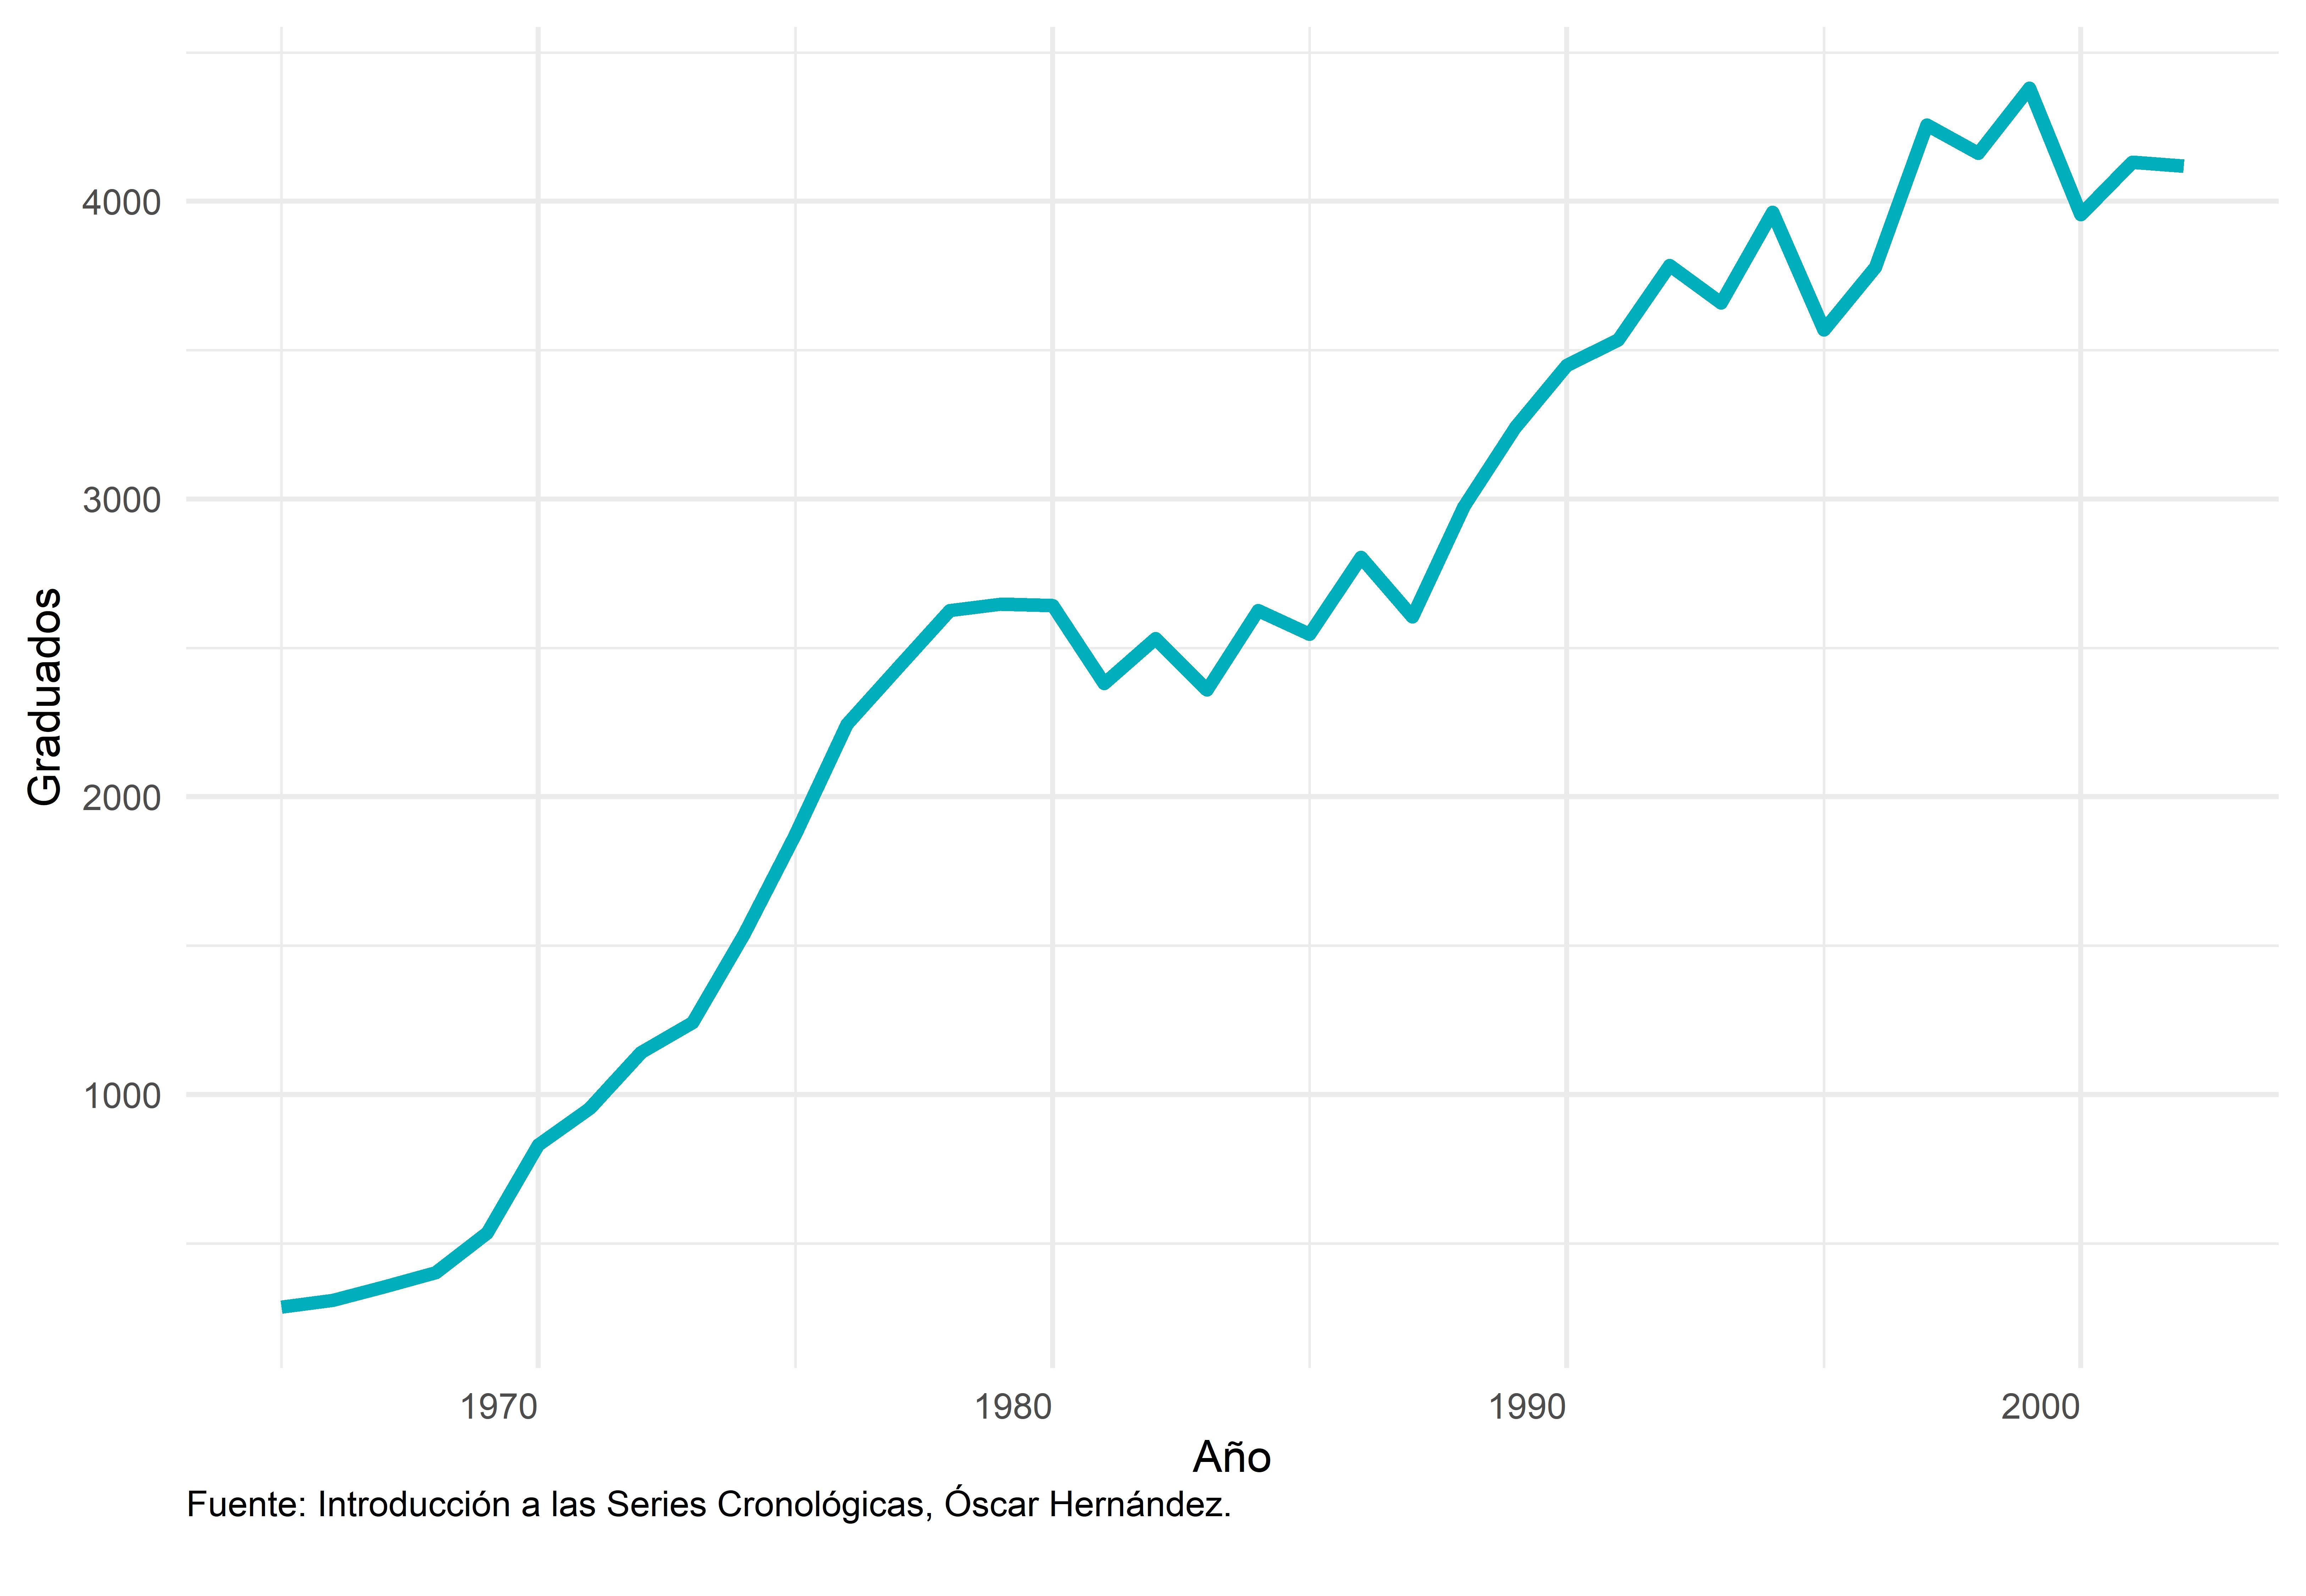
\includegraphics[width=1\linewidth,height=1\textheight]{Tesis_files/figure-latex/ejemplo_ucr-1} \caption{Número anual de graduados de la Universidad de Costa Rica para el periodo 1965-2002}\label{fig:ejemplo_ucr}
\end{figure}

Tal y como menciona el autor, la serie cronológica posee una clara
tendencia creciente a lo largo del tiempo, lo cual sugiere que no se
trata de una serie estacionaria. Esto se confirma al analizar las
funciones de autocorrelación simple y parcial de la serie cronológica en
las Figuras \ref{fig:auto_ucr1} y \ref{fig:parcial_ucr1}; pues la
función de autocorrelación no cae rápidamente a cero, sino que posee un
descenso más pausado.

\begin{figure}[H]
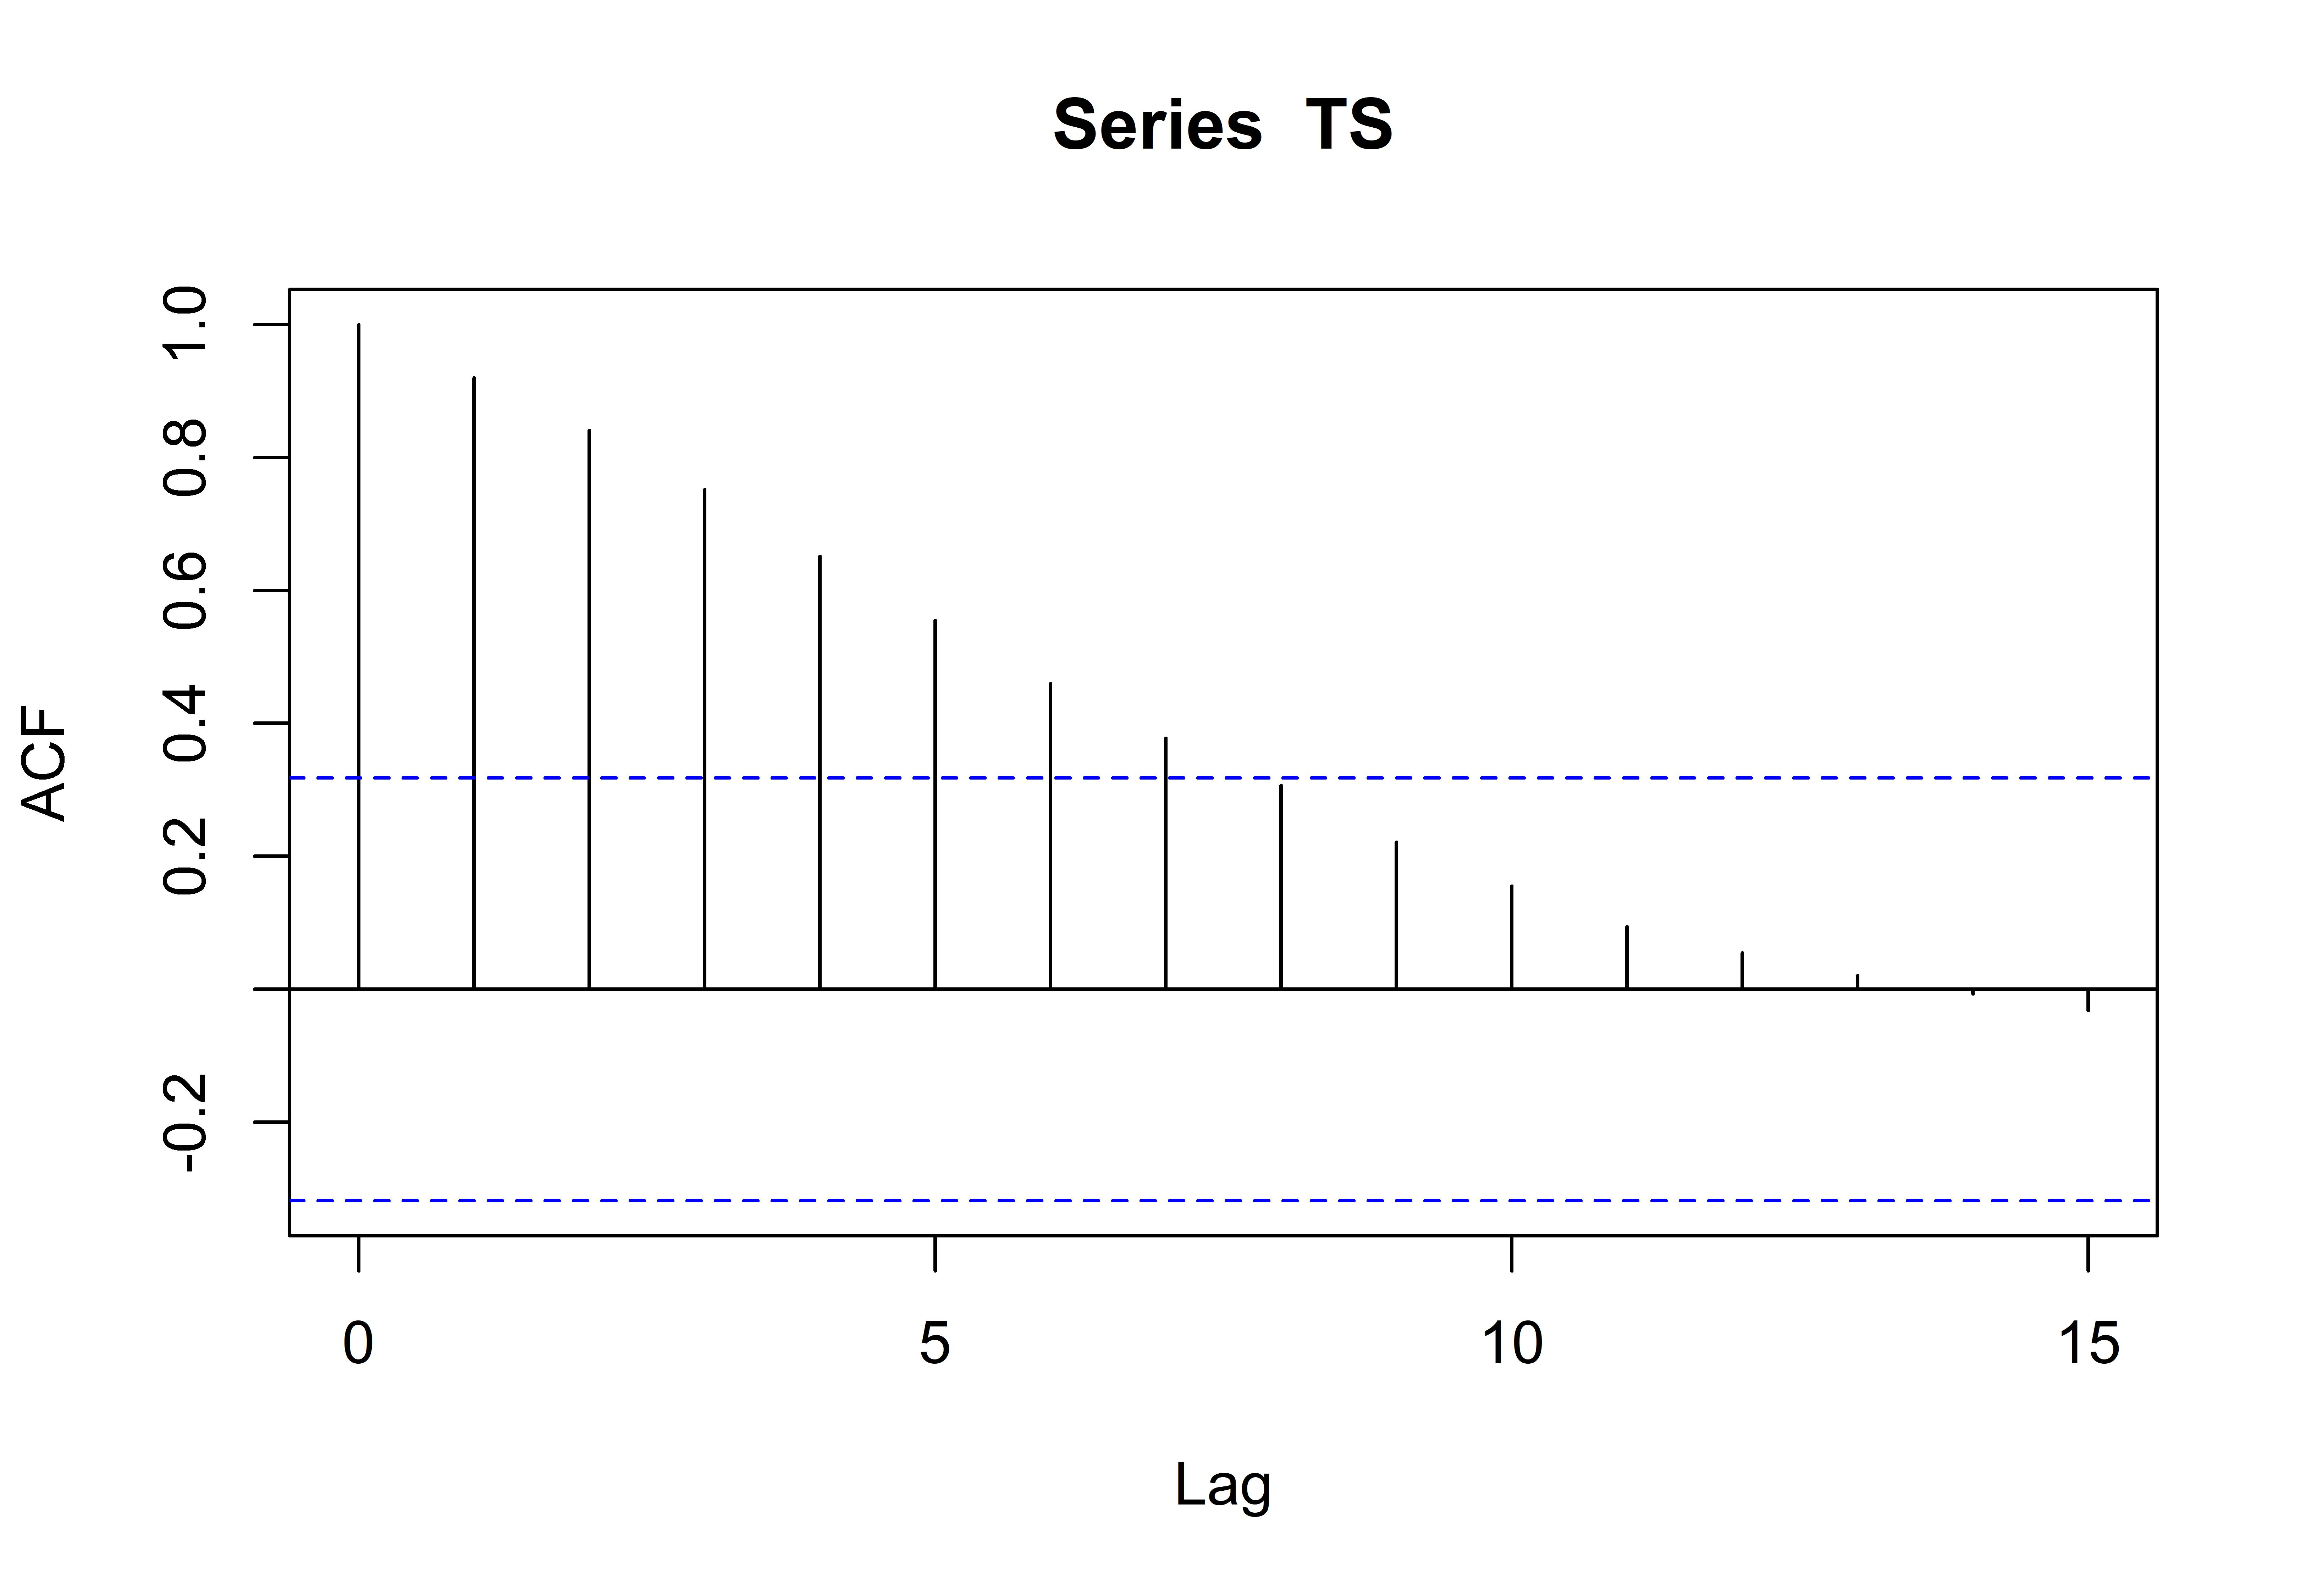
\includegraphics[width=1\linewidth,height=1\textheight]{Tesis_files/figure-latex/auto_ucr1-1} \caption{Función de autocorrelación simple de la serie de graduados de la UCR}\label{fig:auto_ucr1}
\end{figure}

\begin{figure}[H]
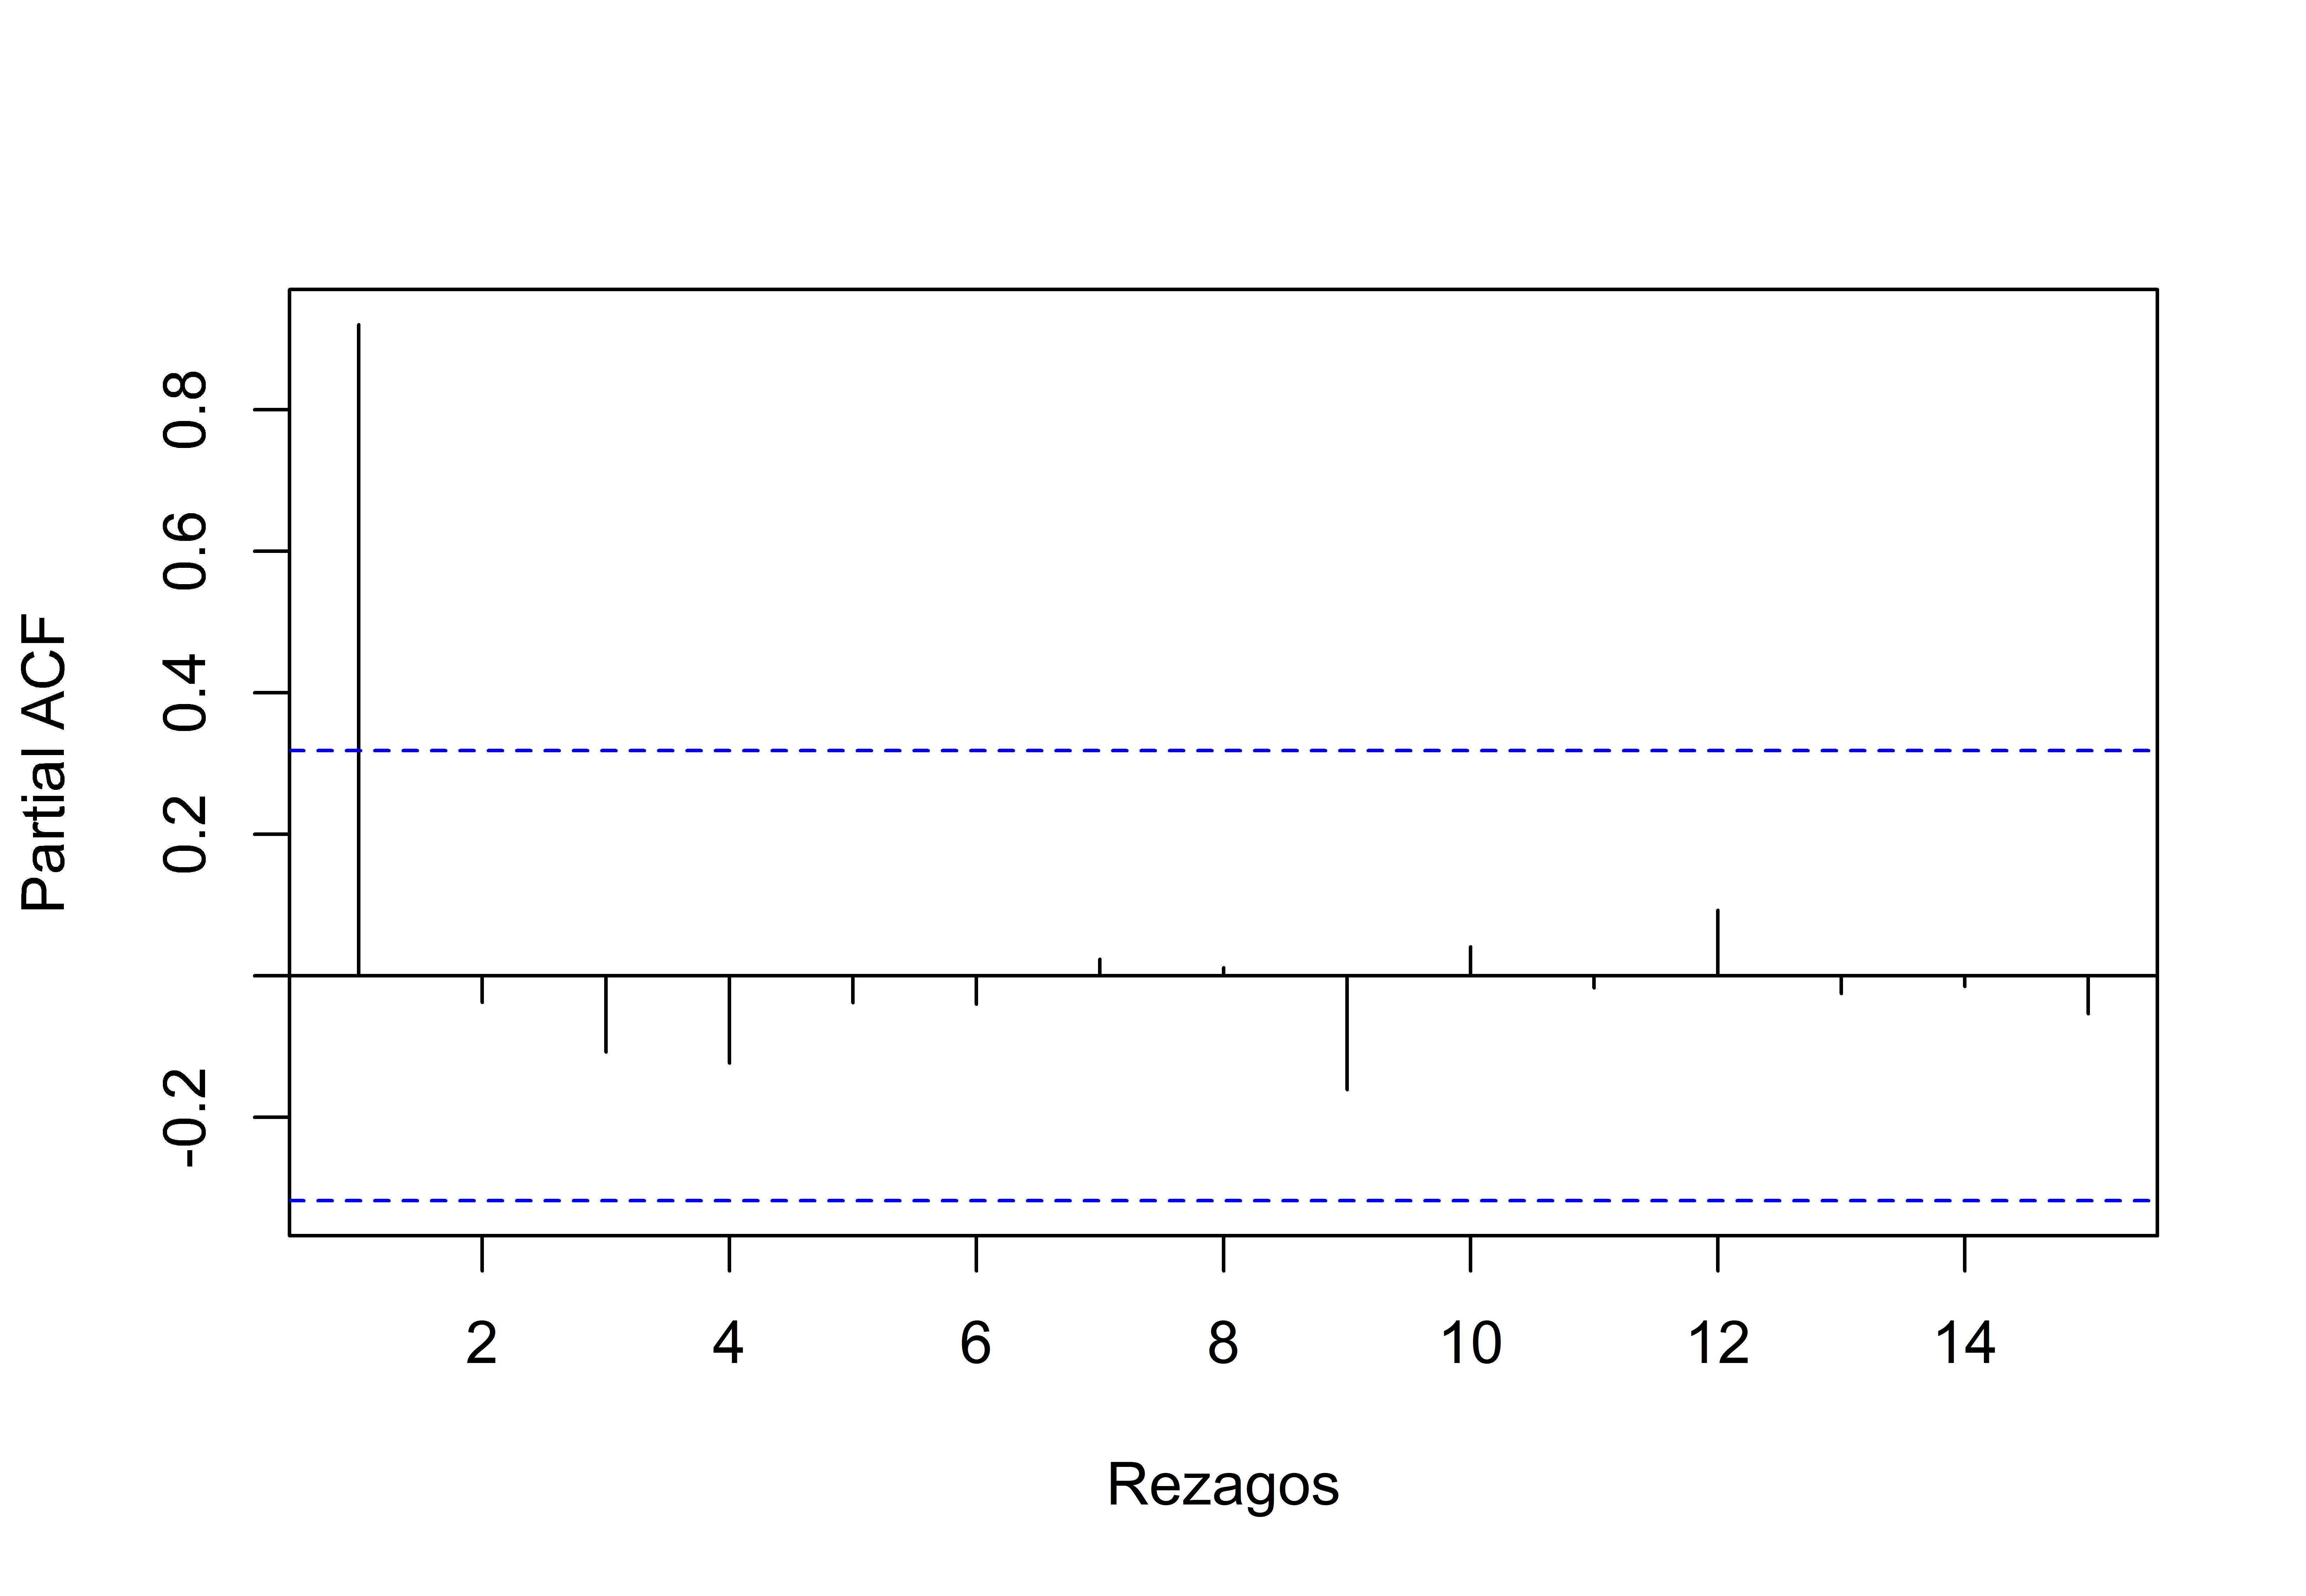
\includegraphics[width=1\linewidth,height=1\textheight]{Tesis_files/figure-latex/parcial_ucr1-1} \caption{Función de autocorrelación parcial de la serie de graduados de la UCR}\label{fig:parcial_ucr1}
\end{figure}

Dado que la serie mostrada no es estacionaria, es posible aplicar una
diferenciación para hacerla cumplir esta condición, tal y como se
muestra en la Figura \ref{fig:ejemplo_ucr_diferenciada}. Al analizar la
Figura \ref{fig:auto_ucr2} se observa cómo la función de autocorrelación
cae rápidamente a cero, lo cual confirma que se posee una serie
estacionaria. Posteriormente, para intentar identificar el proceso que
gobierna la serie cronológica, puede verse que hay dos barras en la
Figura \ref{fig:parcial_ucr2} y que además la función de autocorrelación
de la Figura \ref{fig:auto_ucr2} cae rápidamente hacia cero, lo cual
sugiere que se está en presencia de un modelo autorregresivo de orden 2.

\begin{figure}[H]
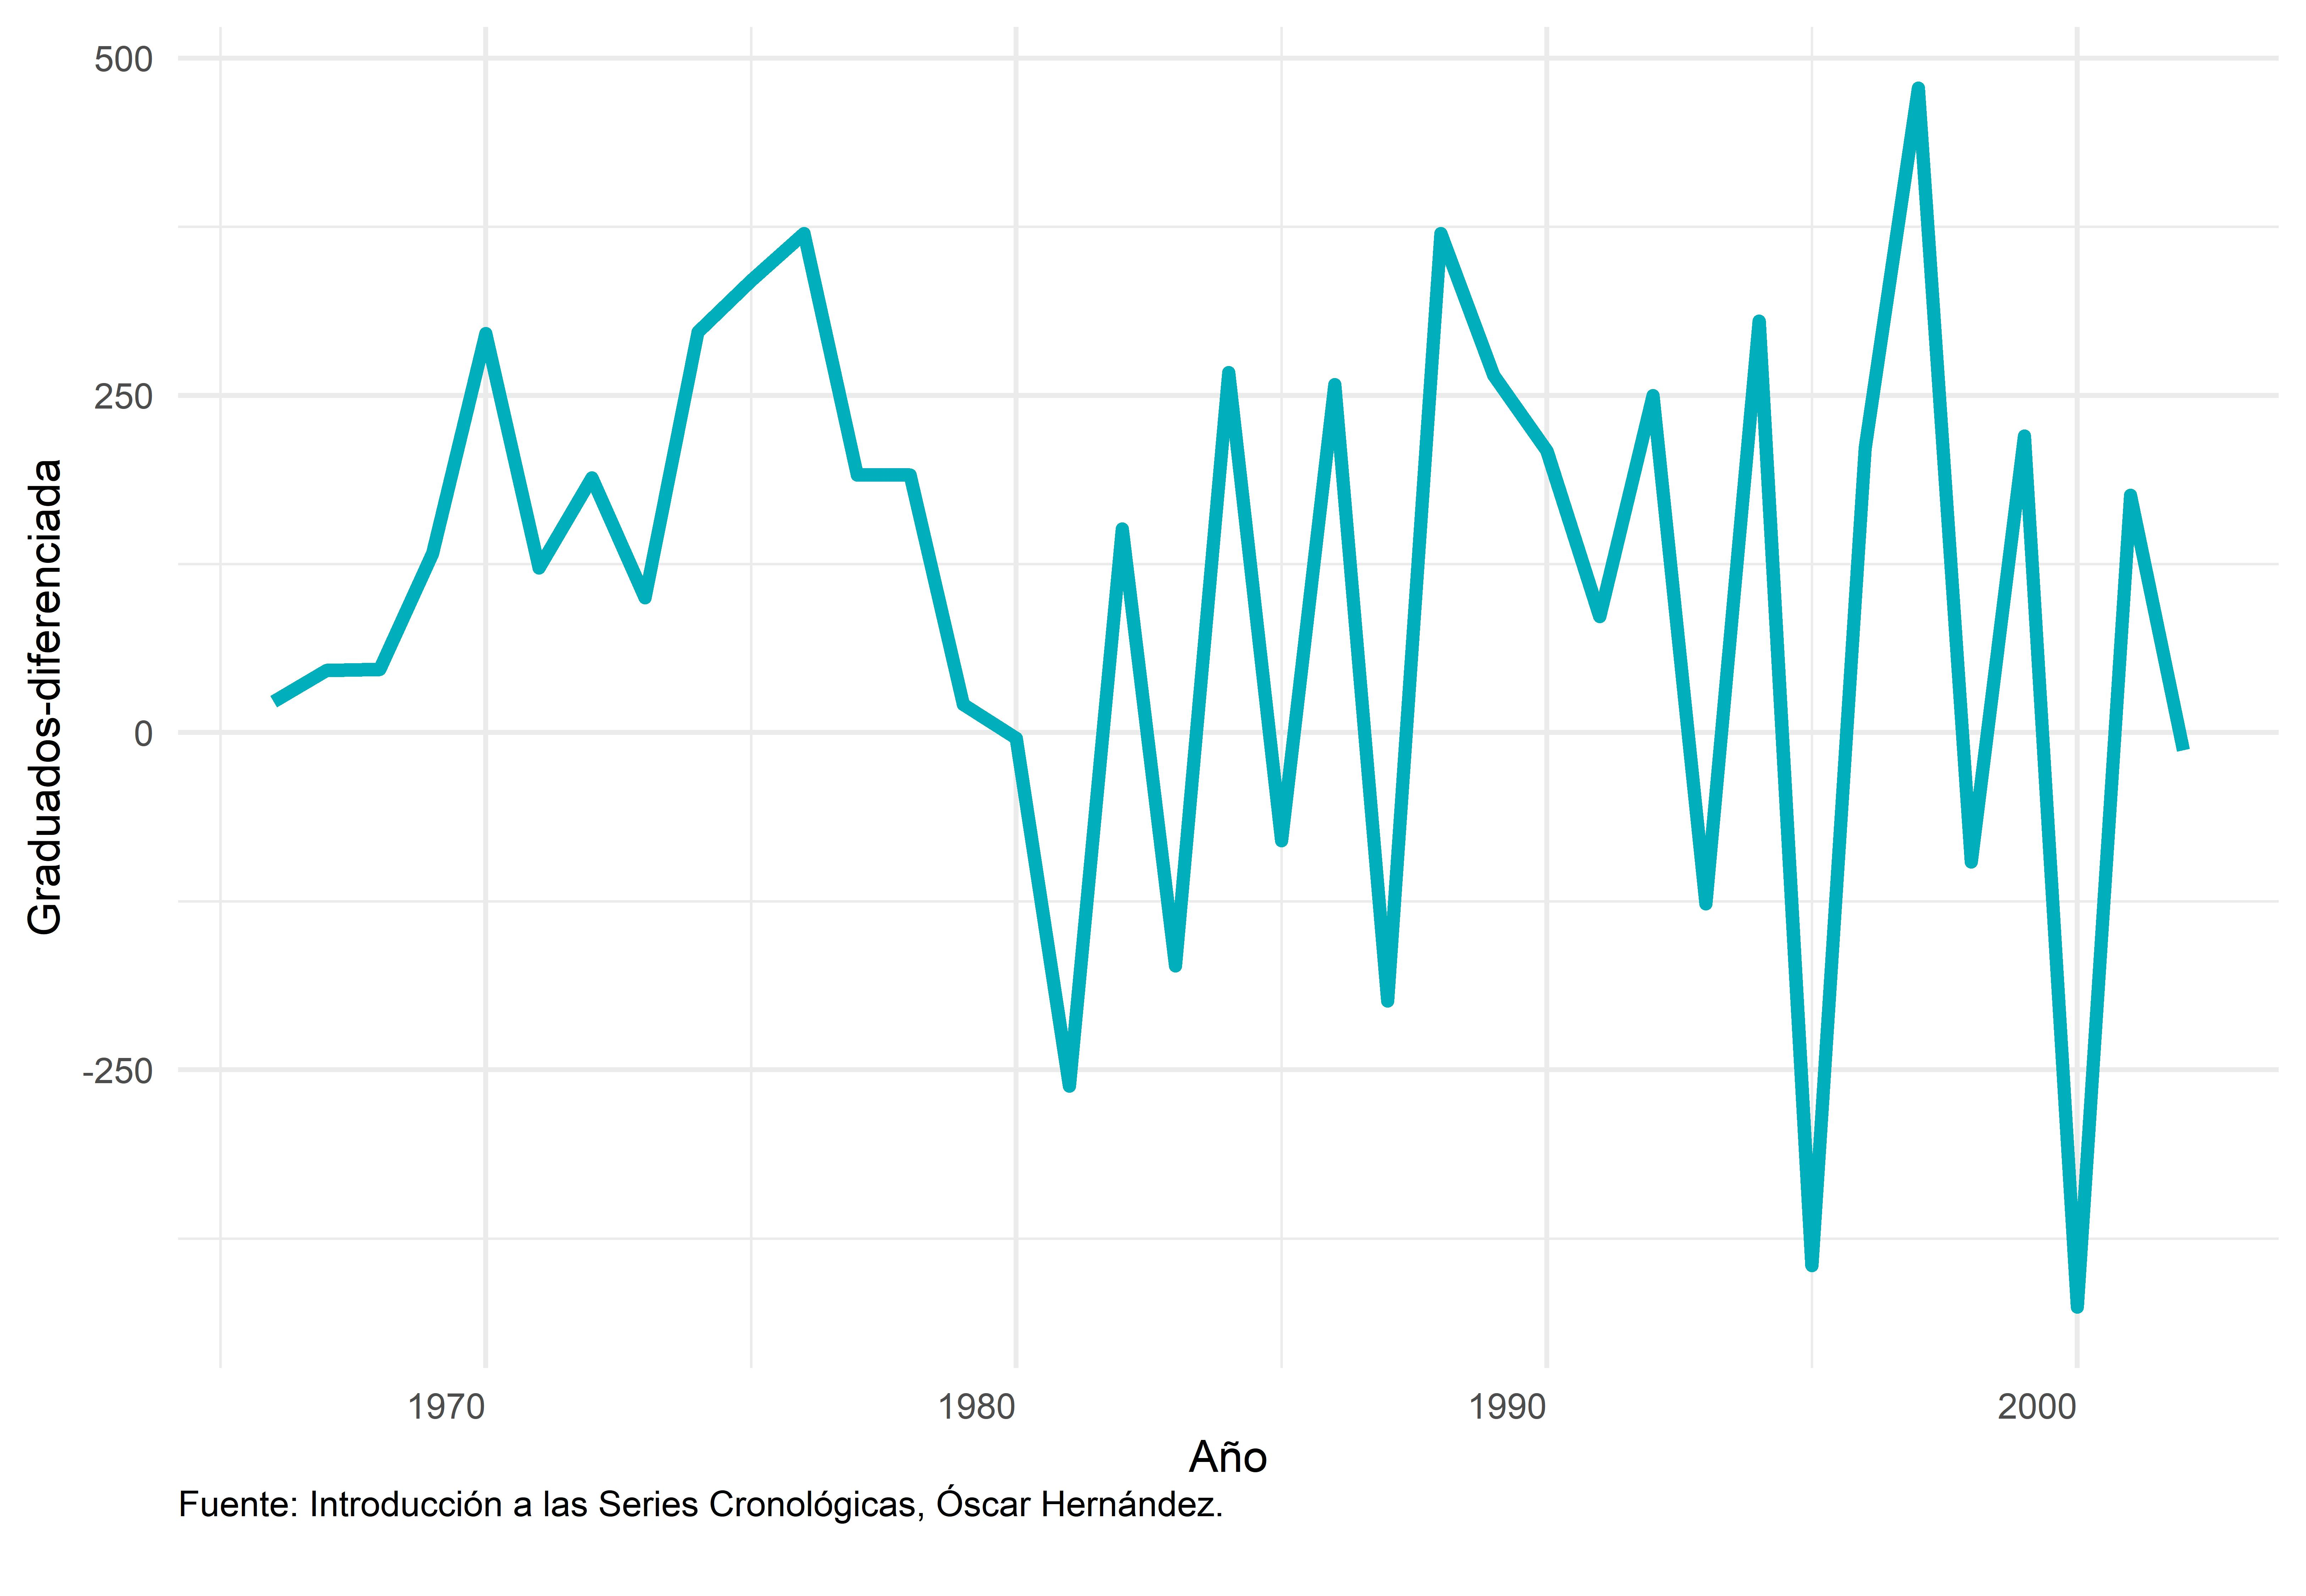
\includegraphics[width=1\linewidth,height=1\textheight]{Tesis_files/figure-latex/ejemplo_ucr_diferenciada-1} \caption{Serie diferenciada de graduados de la Universidad de Costa Rica para el periodo 1965-2002}\label{fig:ejemplo_ucr_diferenciada}
\end{figure}

\begin{figure}[H]
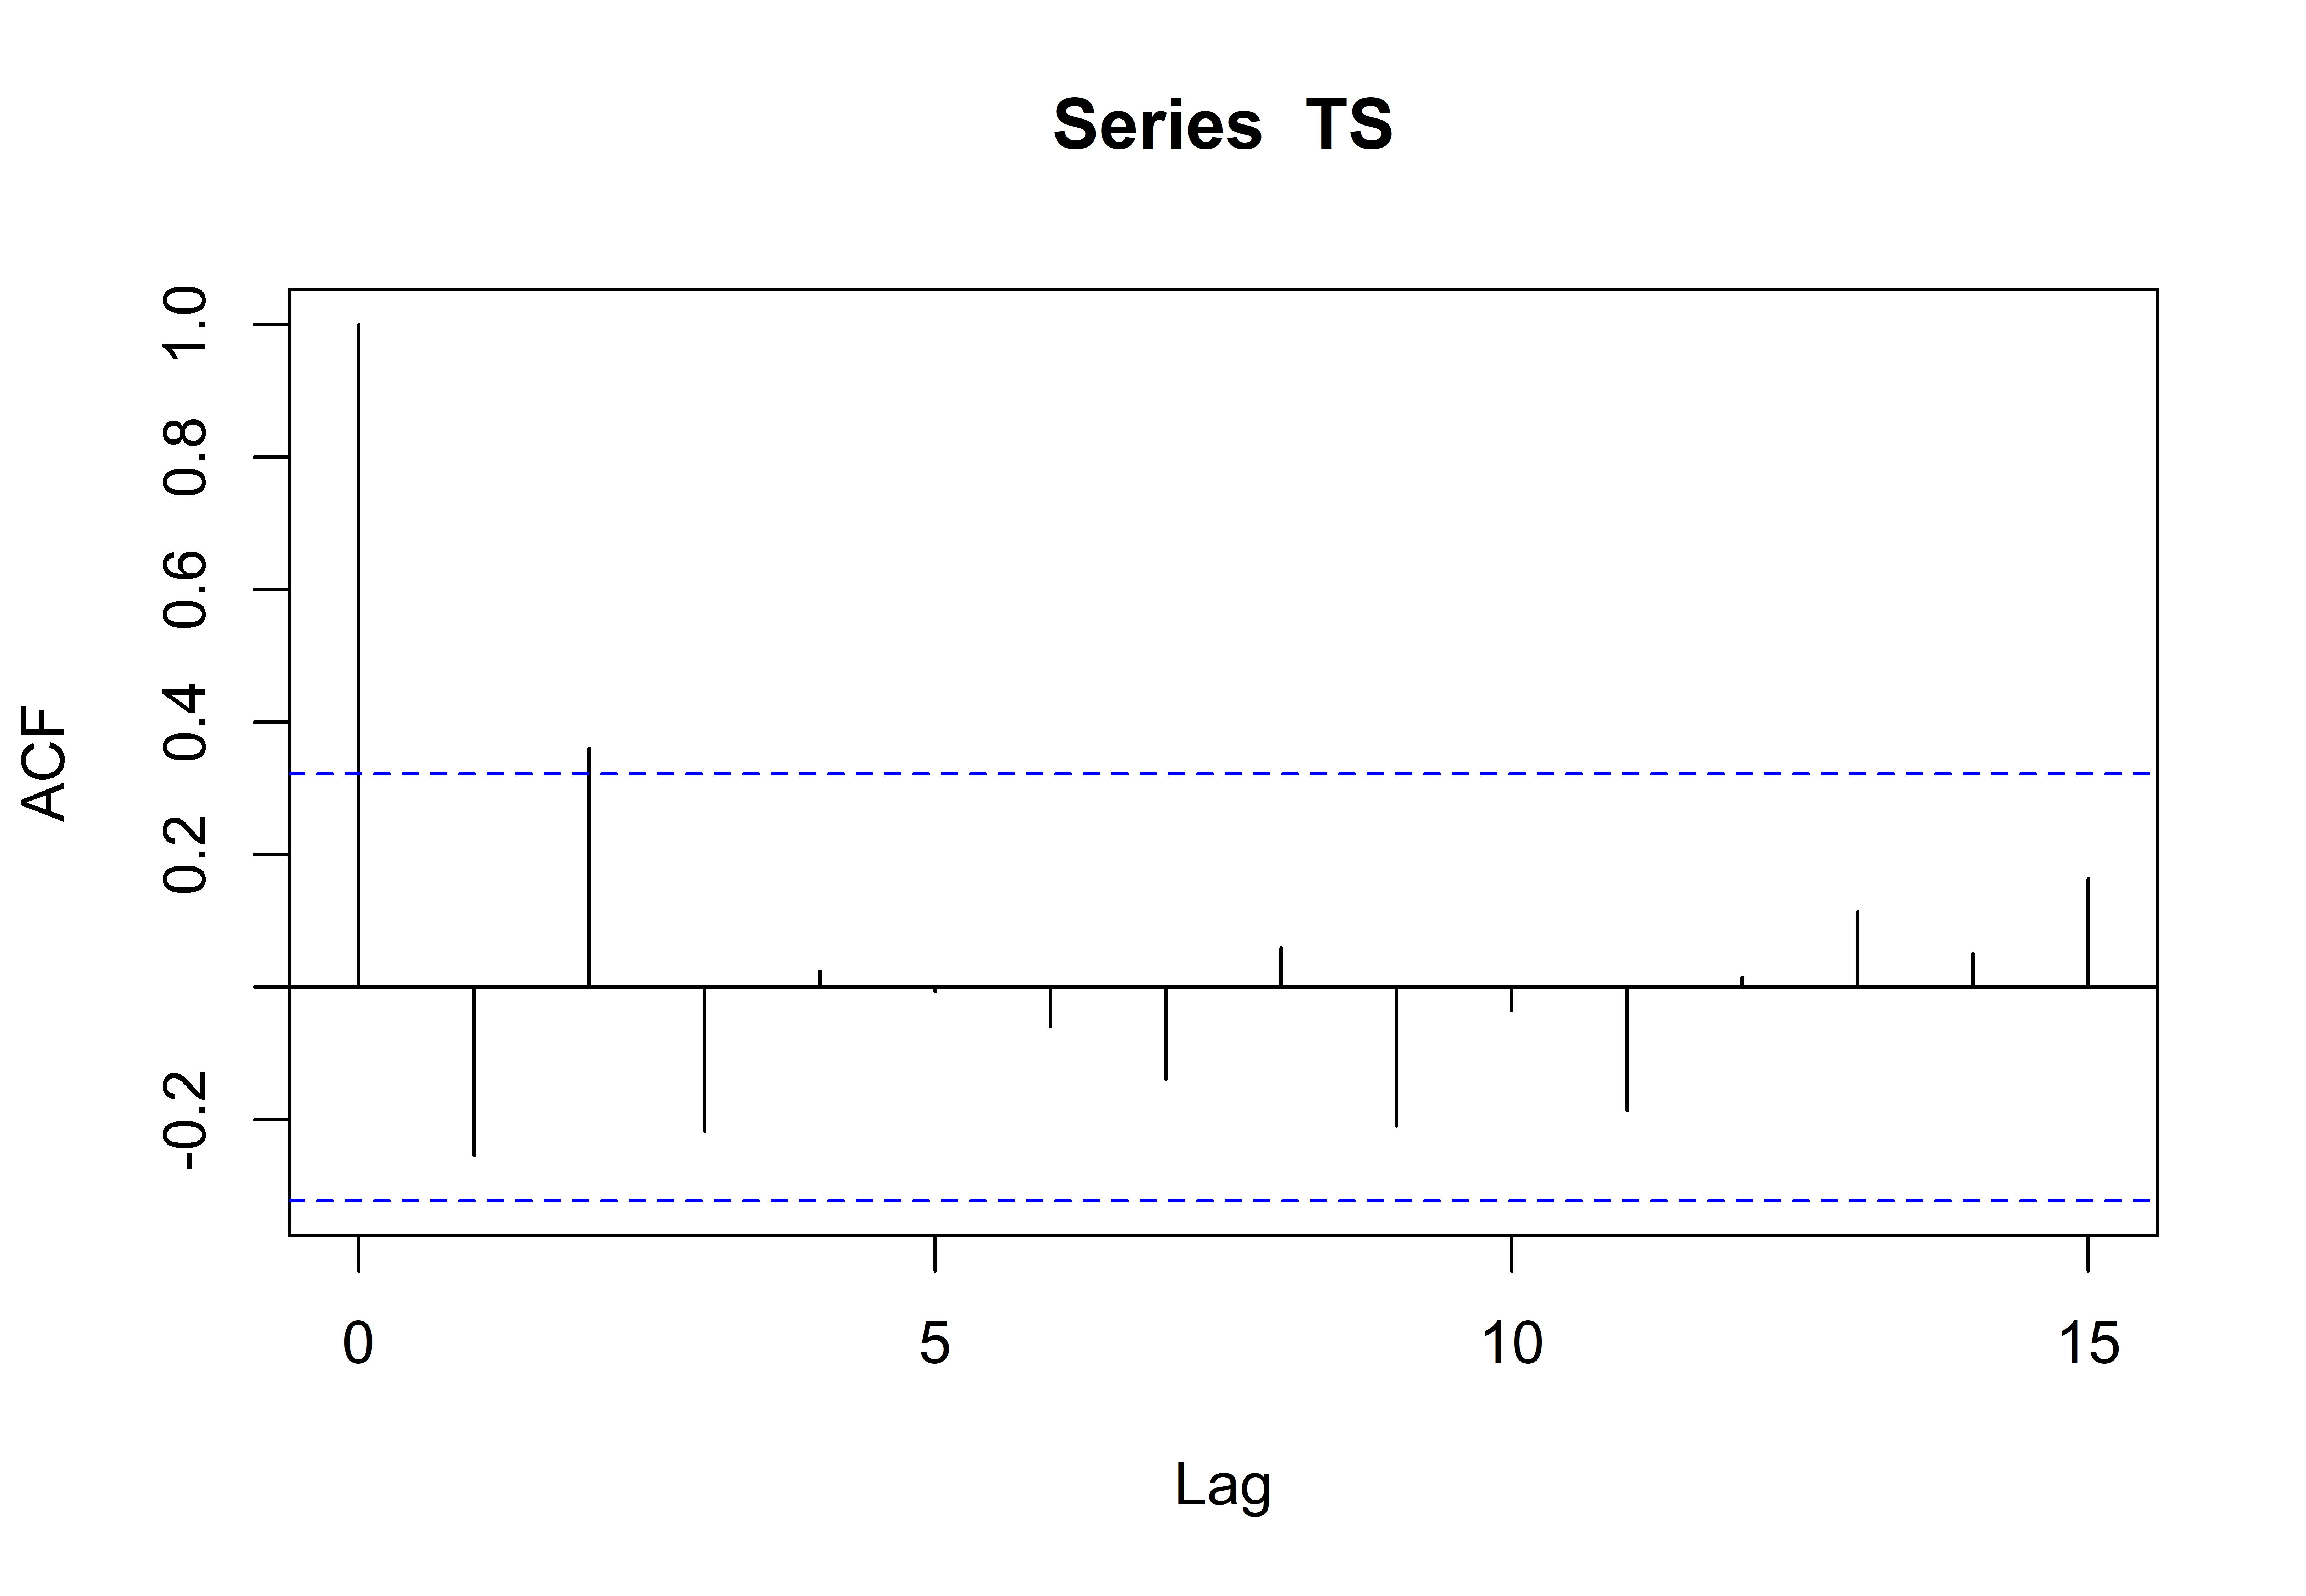
\includegraphics[width=1\linewidth,height=1\textheight]{Tesis_files/figure-latex/auto_ucr2-1} \caption{Función de autocorrelación simple de la serie diferenciada de graduados de la UCR}\label{fig:auto_ucr2}
\end{figure}

\begin{figure}[H]
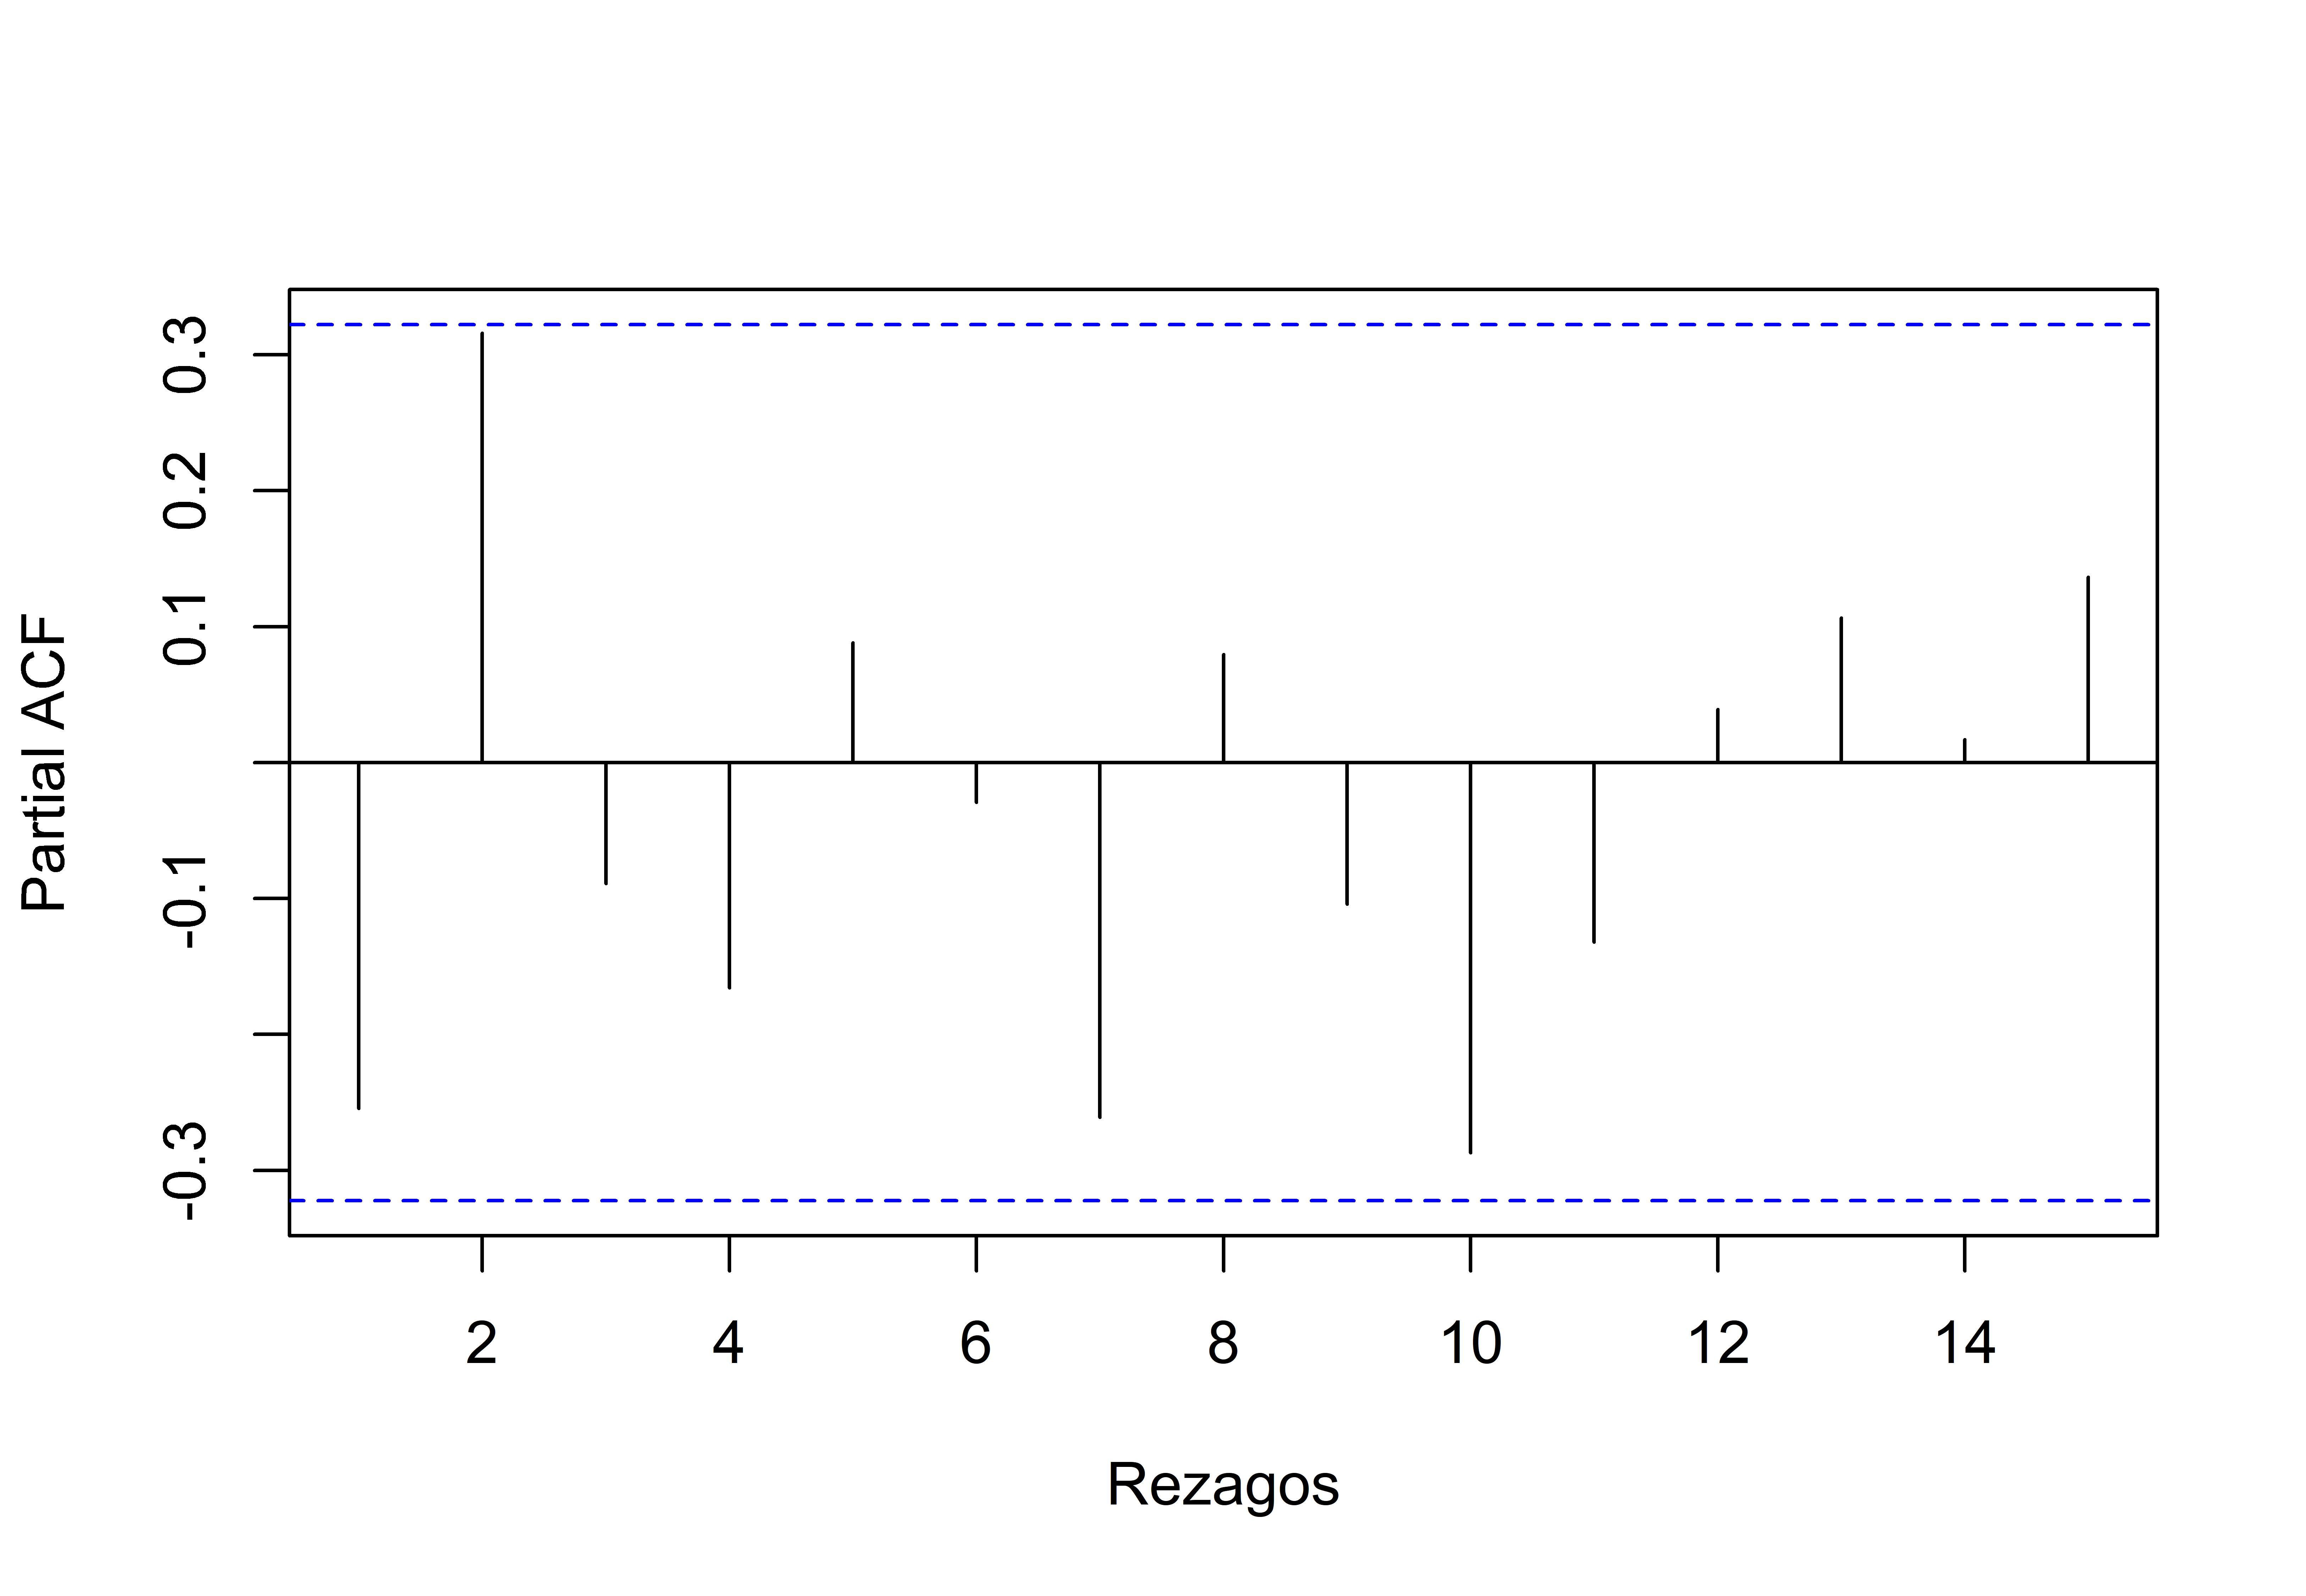
\includegraphics[width=1\linewidth,height=1\textheight]{Tesis_files/figure-latex/parcial_ucr2-1} \caption{Función de autocorrelación parcial de la serie diferenciada de graduados de la UCR}\label{fig:parcial_ucr2}
\end{figure}

Tener en consideración estos y otros posibles criterios para la
identificación del proceso que gobierna la serie cronológica puede
fácilmente volverse subjetivo, pues dos personas diferentes pueden
llegar a dar distintas interpretaciones a las visualizaciones de los
autocorrelogramas. Estas interpretaciones pueden sesgar la
identificación de los modelos y, además, no considerar otros escenarios
para los términos de un modelo \(ARIMA\); para solventar esto es
necesario considerar un abanico más amplio de opciones que a su vez
elimine el criterio subjetivo del observador, lo cual se puede lograr al
considerar múltiples permutaciones de términos para contrastar una gran
cantidad de modelos, es decir, utilizar la sobreparametrización.

\subsection{La sobreparametrización y el análisis combinatorio}

La identificación visual mediante los autocorrelogramas puede llevar a
decisiones erradas acerca del proceso que gobierna la serie cronológica.
Una alternativa es considerar estimaciones de procesos de ordenes bajos,
como un \(ARMA(1,1)\) y poco a poco ir incorporando términos, este
proceso de revisión permite encontrar los puntos en que agregar un
coeficiente más al modelo no aporta ninguna mejora en los resultados del
pronóstico, y así considerar únicamente aquellos modelos que tengan
coeficientes con un aporte estadísticamente significativo. Este
procedimiento es conocido como sobreparametrización. Dependiendo de la
cantidad de observaciones y del rango con que se trabajen los
coeficientes, la comparación de los modelos puede volverse muy extensa y
complicada, razón por la cual resulta imperativo generar un
procedimiento sistemático que logre seleccionar el mejor modelo con base
en sus medidas de ajuste y rendimiento.

Es aquí donde entra en escena el análisis combinatorio, pues a partir de
sus procedimientos es posible conocer la cantidad de modelos que deben
ser probados. Resulta pertinente discutir dos principios fundamentales
del análisis combinatorio mencionados por
\protect\hyperlink{ref-analisis_combinatorio}{Hernández}
(\protect\hyperlink{ref-analisis_combinatorio}{2008}): Uno es el
principio de adición, el cual indica que si se tienen dos procedimientos
\(A\) y \(B\), los cuales pueden realizarse de \(k_A\) y \(k_B\)
maneras, respectivamente, entonces la cantidad de maneras que se puede
realizar uno u otro procedimiento es \(k_A + k_B\). Por otro lado se
tiene el principio de multiplicación, con el cual, si el procedimiento
\(A\) se puede realizar de \(k_A\) formas distintas, seguido de otro
procedimiento \(B\) que puede realizarse de \(k_B\) formas, entonces si
a cada forma de realizar el procedimiento \(A\) se puede asociar a
cualquiera de las \(k_B\) maneras de realizar el procedimiento \(B\),
entonces ambos procedimientos pueden realizarse de \(k_A \cdot k_B\)
formas distintas.

Es a partir de estos dos principios que pueden obtenerse la cantidad de
formas distintas que pueden ordenarse \(m\) elementos tomando \(r\)
elementos a la vez. Uno de ellos son las permutaciones, descritos en la
ecuación \ref{eqn:permutacion}, la cual describe la forma de calcular la
cantidad de formas distintas que puede ordenarse \(m\) elementos tomando
\(r\) a la vez, donde el orden sí importa, a modo de ejemplo, si se
quiere saber la cantidad formas que pueden ordenarse las letras \(A, B\)
y \(C\) tomando dos letras a la vez, se tendría que existen
\(\frac{3!}{(3-1)!}=6\) formas distintas, que son \(AB, AC, BC, BA, CA\)
y \(CB\). De manera similar, se tienen las combinaciones, cuya fórmula
se describe en la ecuación \ref{eqn:combinacion}, que brinda la cantidad
de maneras distintas en que pueden ordenarse \(m\) elementos tomando
\(r\) a la vez donde el orden no importa; es decir, si se desean ordenar
las letras \(A, B\) y \(C\) tomando dos a la vez, se tendrían
\(\frac{3!}{2!(3-1)!}=3\) formas distintas, las cuales son \(AB, AC\) y
\(BC\).

\begin{equation}
\label{eqn:permutacion}
_mP_r=\frac{m!}{(m-r)!}
\end{equation}

\begin{equation}
\label{eqn:combinacion}
_mC_r=\frac{m!}{r!(m-r)!}
\end{equation}

Es a partir de esto que la sobreparametrización se utiliza en conjunto
con el análisis combinatorio y en particular con el método de
permutaciones, pues el orden de la cantidad de coeficientes a estimar en
un modelo \(ARIMA(p,d,q)\) sí importa, debido a que no es lo mismo
estimar un modelo \(ARIMA(2,1,3)\) que un modelo \(ARIMA(3,1,2)\). En
las elección de modelos ARIMA normalmente los métodos tradicionales como
los correlogramas u otros, no suelen abarcar un espectro más amplio de
coeficientes, y esto podría representar un método de estimación que no
es el mejor, por esto, la presente tesis propone una metodología que
mezcla la sobreparametrización con las permutaciones con el objetivo de
lograr estimar el mejor modelo \(ARIMA\) de una amplia cantidad de
posibles candidatos para conseguir pronósticos más precisos en
comparación a los métodos tradicionales.

\newpage

\section{METODOLOGÍA}

La aplicación de las series cronológicas tiene tres objetivos: 1) el
análisis exploratorio de la serie en cuestión, 2) estimar modelos de
proyección, y 3) generar pronósticos para los posibles valores futuros
que tomará la serie cronológica.

Esta sección aborda la metodología propuesta como método de estimación y
pronóstico de series cronológicas. En la búsqueda de un modelo adecuado
de entre varios candidatos, se cubren en un primer apartado los
materiales a utilizar, así como los métodos, incluyendo el proceso de
estimación, el procedimiento de simulación empleado para la verificación
del método propuesto, y las medidas de bondad de ajuste y de precisión a
utilizar. Se describe en detalle el uso de la sobreparametrización como
herramienta para la generación de pronósticos de series cronológicas con
temporalidades mensuales, bimensuales, trimestrales, cuatrimestrales o
anuales mediante un proceso de selección fundamentada en las
permutaciones de todos los parámetros de un modelo ARIMA hasta un rango
determinado. Las medidas de precisión y de bondad de ajuste sirven de
insumo para utilizar un método de consenso entre ellas y seleccionar el
modelo más adecuado mediante la sobreparametrización: se comparan todos
los posibles modelos en un intervalo específico de términos definiendo
una diferenciación adecuada para la serie y permutando hasta un máximo
definido para los términos autorregresivos y de medias móviles
especificados para así seleccionar la especificación que ofrezca mejores
resultados al momento de pronosticar valores futuros de la serie
cronológica.

\subsection{Materiales}

Se describen a continuación las series cronológicas reales que servirán
de insumo para poner a prueba el método propuesto.

\subsubsection{Tasa de mortalidad infantil interanual}

La Tasa de Mortalidad Infantil (TMI) es uno de los indicadores
demográficos más importantes, pues es utilizado como un parámetro de
referencia sobre la calidad del sistema de salud, tanto a nivel nacional
como regional. Si bien este indicador se construye relacionando las
defunciones de menores de un año con el total de nacimientos, también
involucra de manera implícita otras condiciones tales como las
económicas, sociales y culturales, así como la efectividad en los
métodos preventivos y curativos de esta categoría poblacional
(\protect\hyperlink{ref-leon}{León, 1998}). Debido a esto, el
fallecimiento de un niño menor de un año se traduce en una falla del
sistema de salud, por lo que estos casos son sujetos de estudio con el
fin de conocer las causas que desencadenaron el evento.

En algunos países en vías de desarrollo de Asia, África y América
Latina, la mortalidad infantil alcanza valores elevados pues la
desnutrición, ausencia de asistencia médica y mala calidad de las
condiciones sanitarias son, a diferencia de los países más
desarrollados, algo muy común (\protect\hyperlink{ref-donoso}{Donoso,
2004}). En el caso de Costa Rica, la unidad de estadísticas demográficas
del Instituto Nacional de Estadística y Censos\footnote{\url{http://www.inec.go.cr/}}
(INEC) es el ente encargado de reportar este indicador con el fin de dar
seguimiento y control al comportamiento del mismo a lo largo del tiempo
con el objetivo de llegar a los niveles más bajos posibles.

En el INEC, cada mes se publica el boletín de la TMI interanual (TMII),
que analiza la TMI de un mes y los 11 meses previos para comparar los
periodos correspondientes (\protect\hyperlink{ref-infantiles}{INEC,
2004}). Este apartado busca hacer un análisis de la TMII para los 12
periodos desde el año 1989 y hasta 2017, y no de manera mensual simple,
pues dada la volatilidad del fenómeno de estudio, hacer un estudio
interanual permite analizar de una mejor manera los cambios entre
periodos. Esta forma de definit la TMII genera una autocorrelación
natural en los datos, pues la información utilizada en el momento \(t\)
coincide en alrededor de 92\% con la TMII del mes periodo inmediatemente
anterior. Se analizará entonces la TMII desde el periodo Febrero 1989 --
Enero 1990 hasta el periodo Enero 2017 -- Diciembre 2017.

La importancia de este proceso, aparte de servir de parámetro para
evaluar el sistema de salud, está en su estrecha relación con las
proyecciones de población, pues como se mencionó previamente, la TMII
analiza la mortalidad en el grupo de edad de menores de un año, que es
el primer grupo al generar tablas de mortalidad, ya sea de la forma
clásica o mediante la mortalidad óptima
(\protect\hyperlink{ref-mortalidad_optima}{Villalón, 2006}). Uno de los
métodos más conocidos para realizar estas estimaciones es el método de
los componentes de cambio demográfico, que son la fecundidad, la
mortalidad y la migración. En el caso de la mortalidad, uno de los
puntos de partida es la estimación de las tasas de mortalidad por grupos
de edad, siendo de particular interés la de menores de cinco años, pues
esta a su vez se subdivide en los grupos de menores de un año y el de
uno a cuatro años. Conocer el comportamiento de la mortalidad infantil
es importante porque es en este grupo de edad en el que pueden existir
cambios muy bruscos en la mortalidad y la fecundidad
(\protect\hyperlink{ref-Rincon}{Rincon, 2000}).

Dado que la medición de la TMII se hace partiendo de un determinado mes
y a partir de éste se consideran los 11 meses anteriores, el primer
valor de la base de datos fue medido a partir de Enero de 2000, que
corresponde al período interanual Febrero 1999 -- Enero 2000. Todos los
periodos siguientes se muestran en la Figura \ref{fig:tmiiplotgeneral}.

\begin{figure}[H]
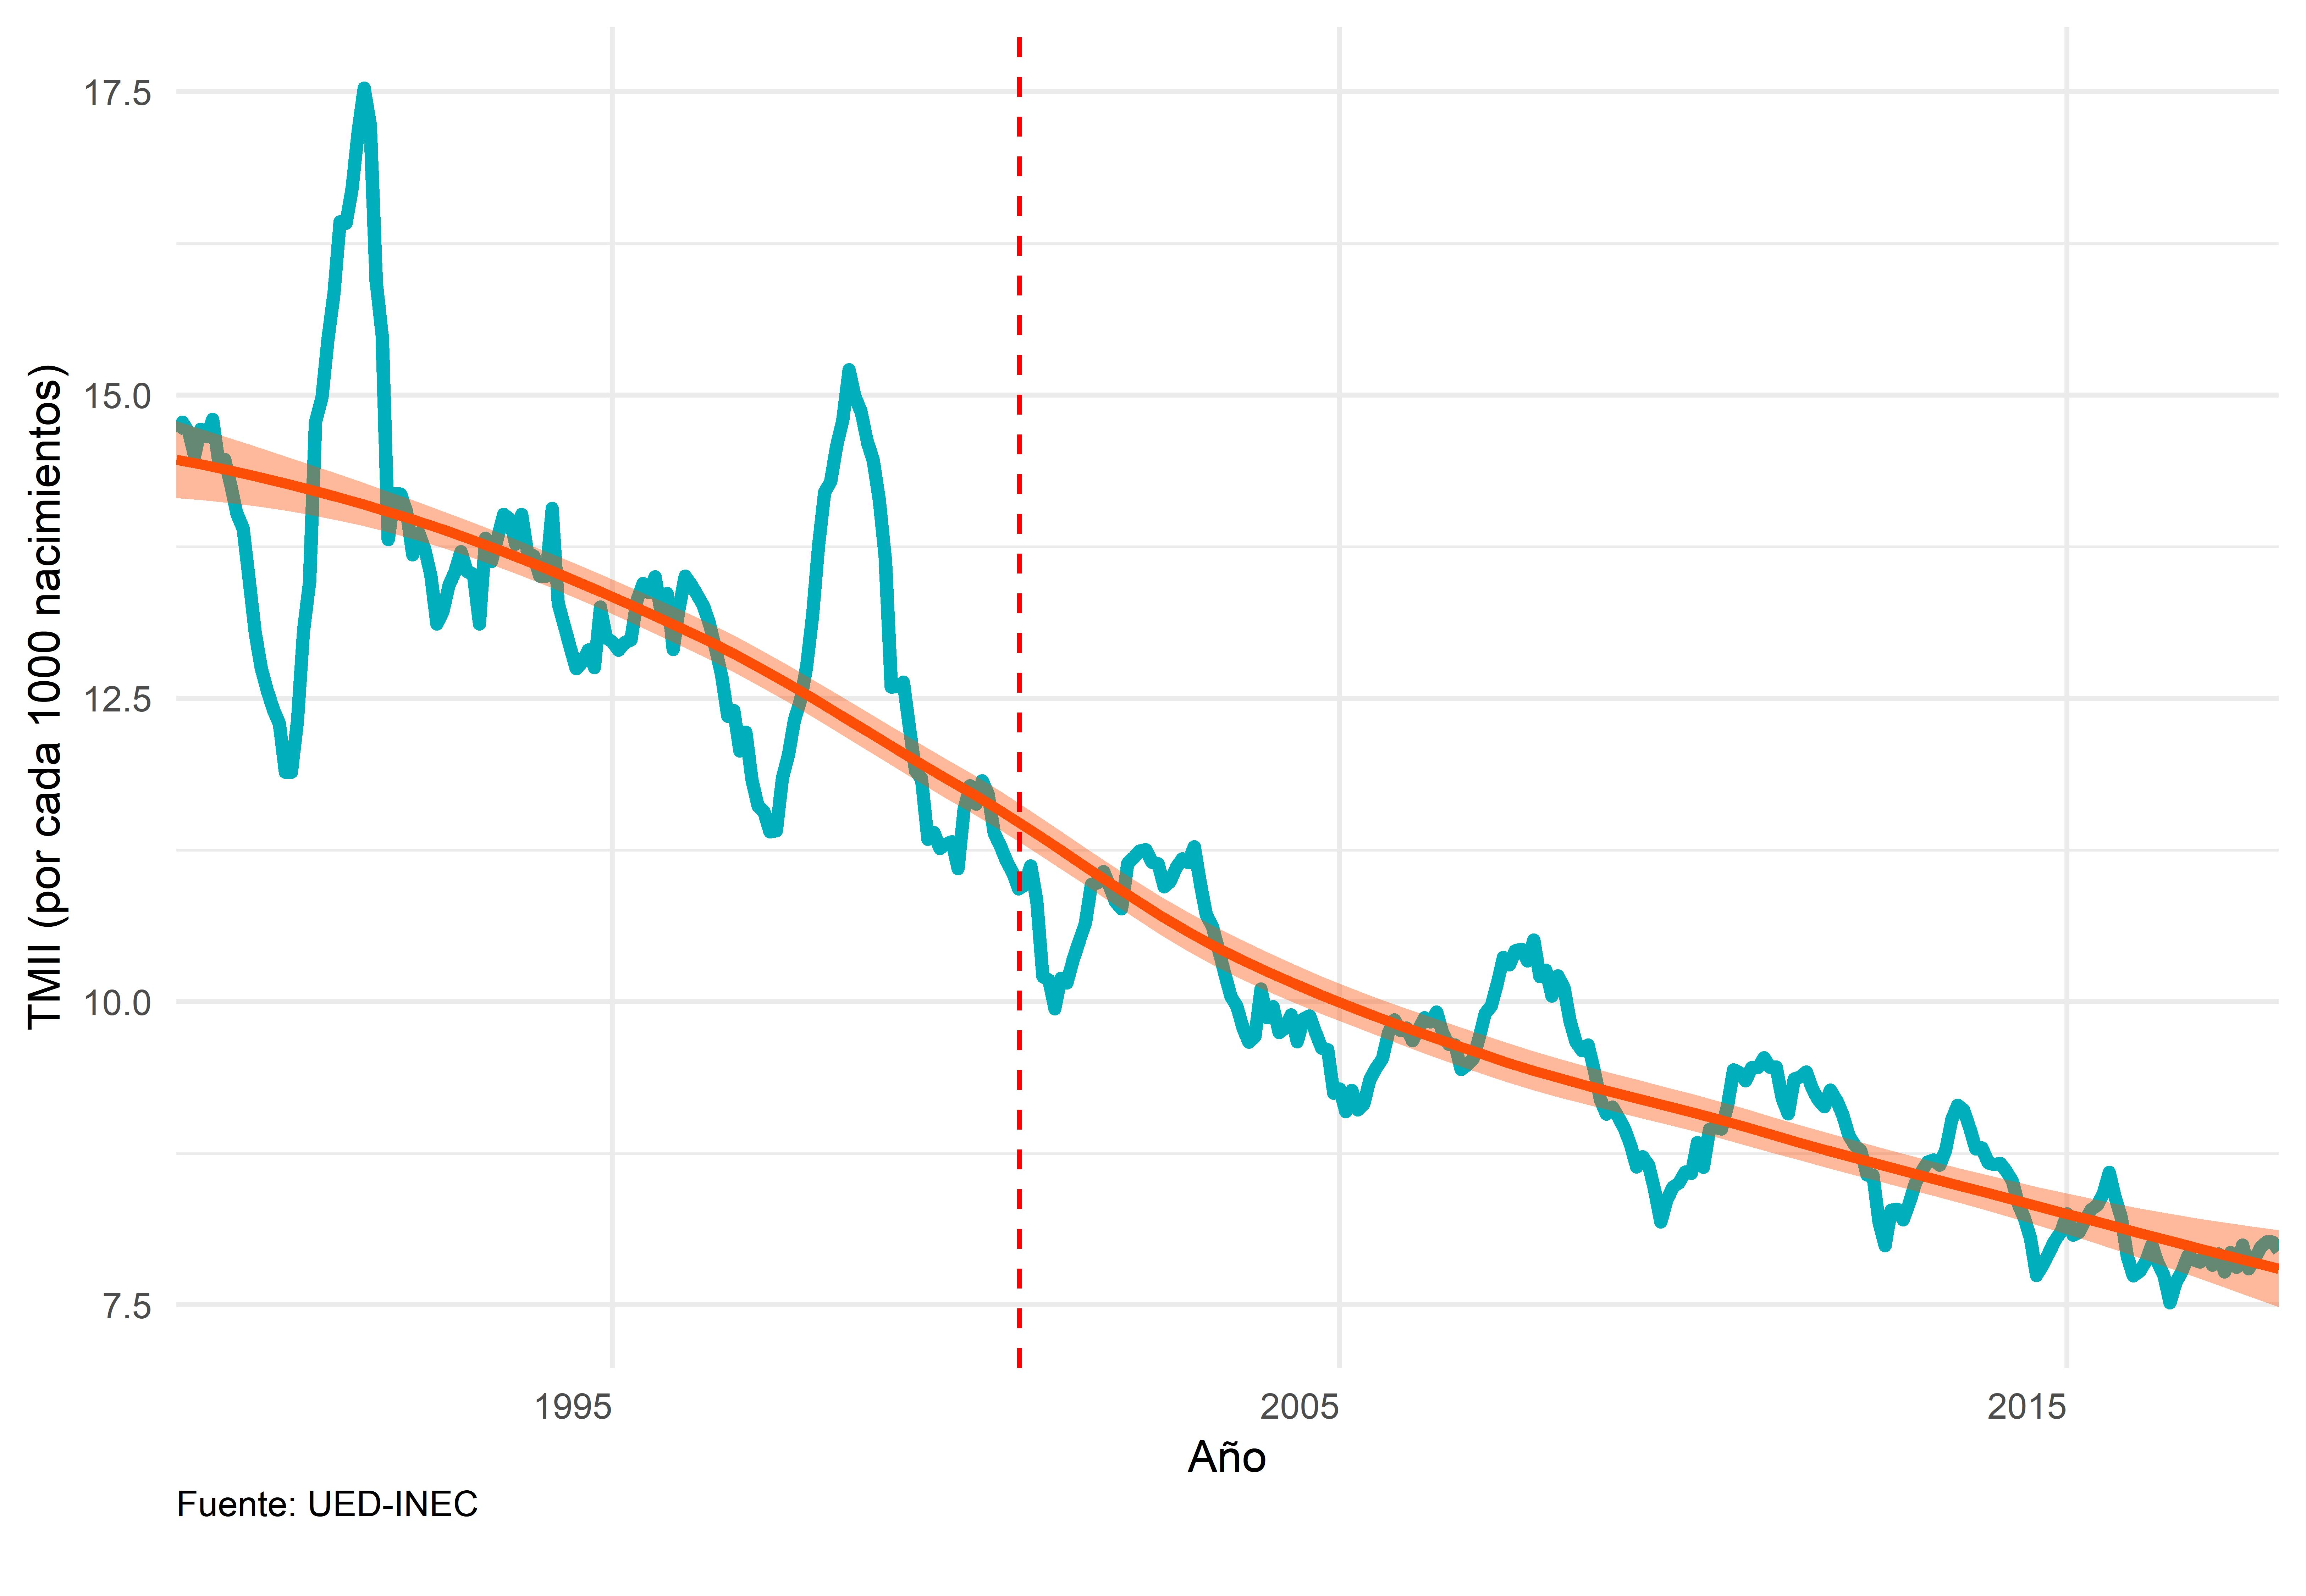
\includegraphics[width=1\linewidth,height=1\textheight]{Tesis_files/figure-latex/tmiiplotgeneral-1} \caption{Tasa de Mortalidad Infantil Interanual 1989 - 2017}\label{fig:tmiiplotgeneral}
\end{figure}

La serie muestra picos y valles pronunciados a lo largo de todo el
periodo. A modo de visualización, se ajustó un suavizamiento de Loess
para buscar señales de tendencia y concavidad en los datos temporales.
La línea roja punteada se ubica aproximadamente en el mes de Julio del
año 2000, pues a partir de ese punto el suavizamiento de Loess muestra
un ligero cambio en la concavidad, lo cual sugiere que a partir ese
punto será más difícil que la TMII vuelva a alcanzar valores similares a
los mostrados al inicio de la serie. Además, al presentarse dos caídas y
subidas abruptas en la TMII, esta tiende a estabilizarse.

Mediante un análisis visual, la Figura \ref{fig:tmiiplotperiodos} parece
respaldar el supuesto de que la mortalidad no posee efectos estacionales
determinantes, pues para cada uno de los 12 períodos, en ninguno parecen
existir mayores diferencias. El efecto que se mantiene en cada uno de
los períodos es el de la tendencia, pues en cada uno ésta sigue
descendiendo con el pasar de los años. Este hecho coincide con lo
observado en la Figura \ref{fig:tmiiplotgeneral}.

\begin{figure}[H]
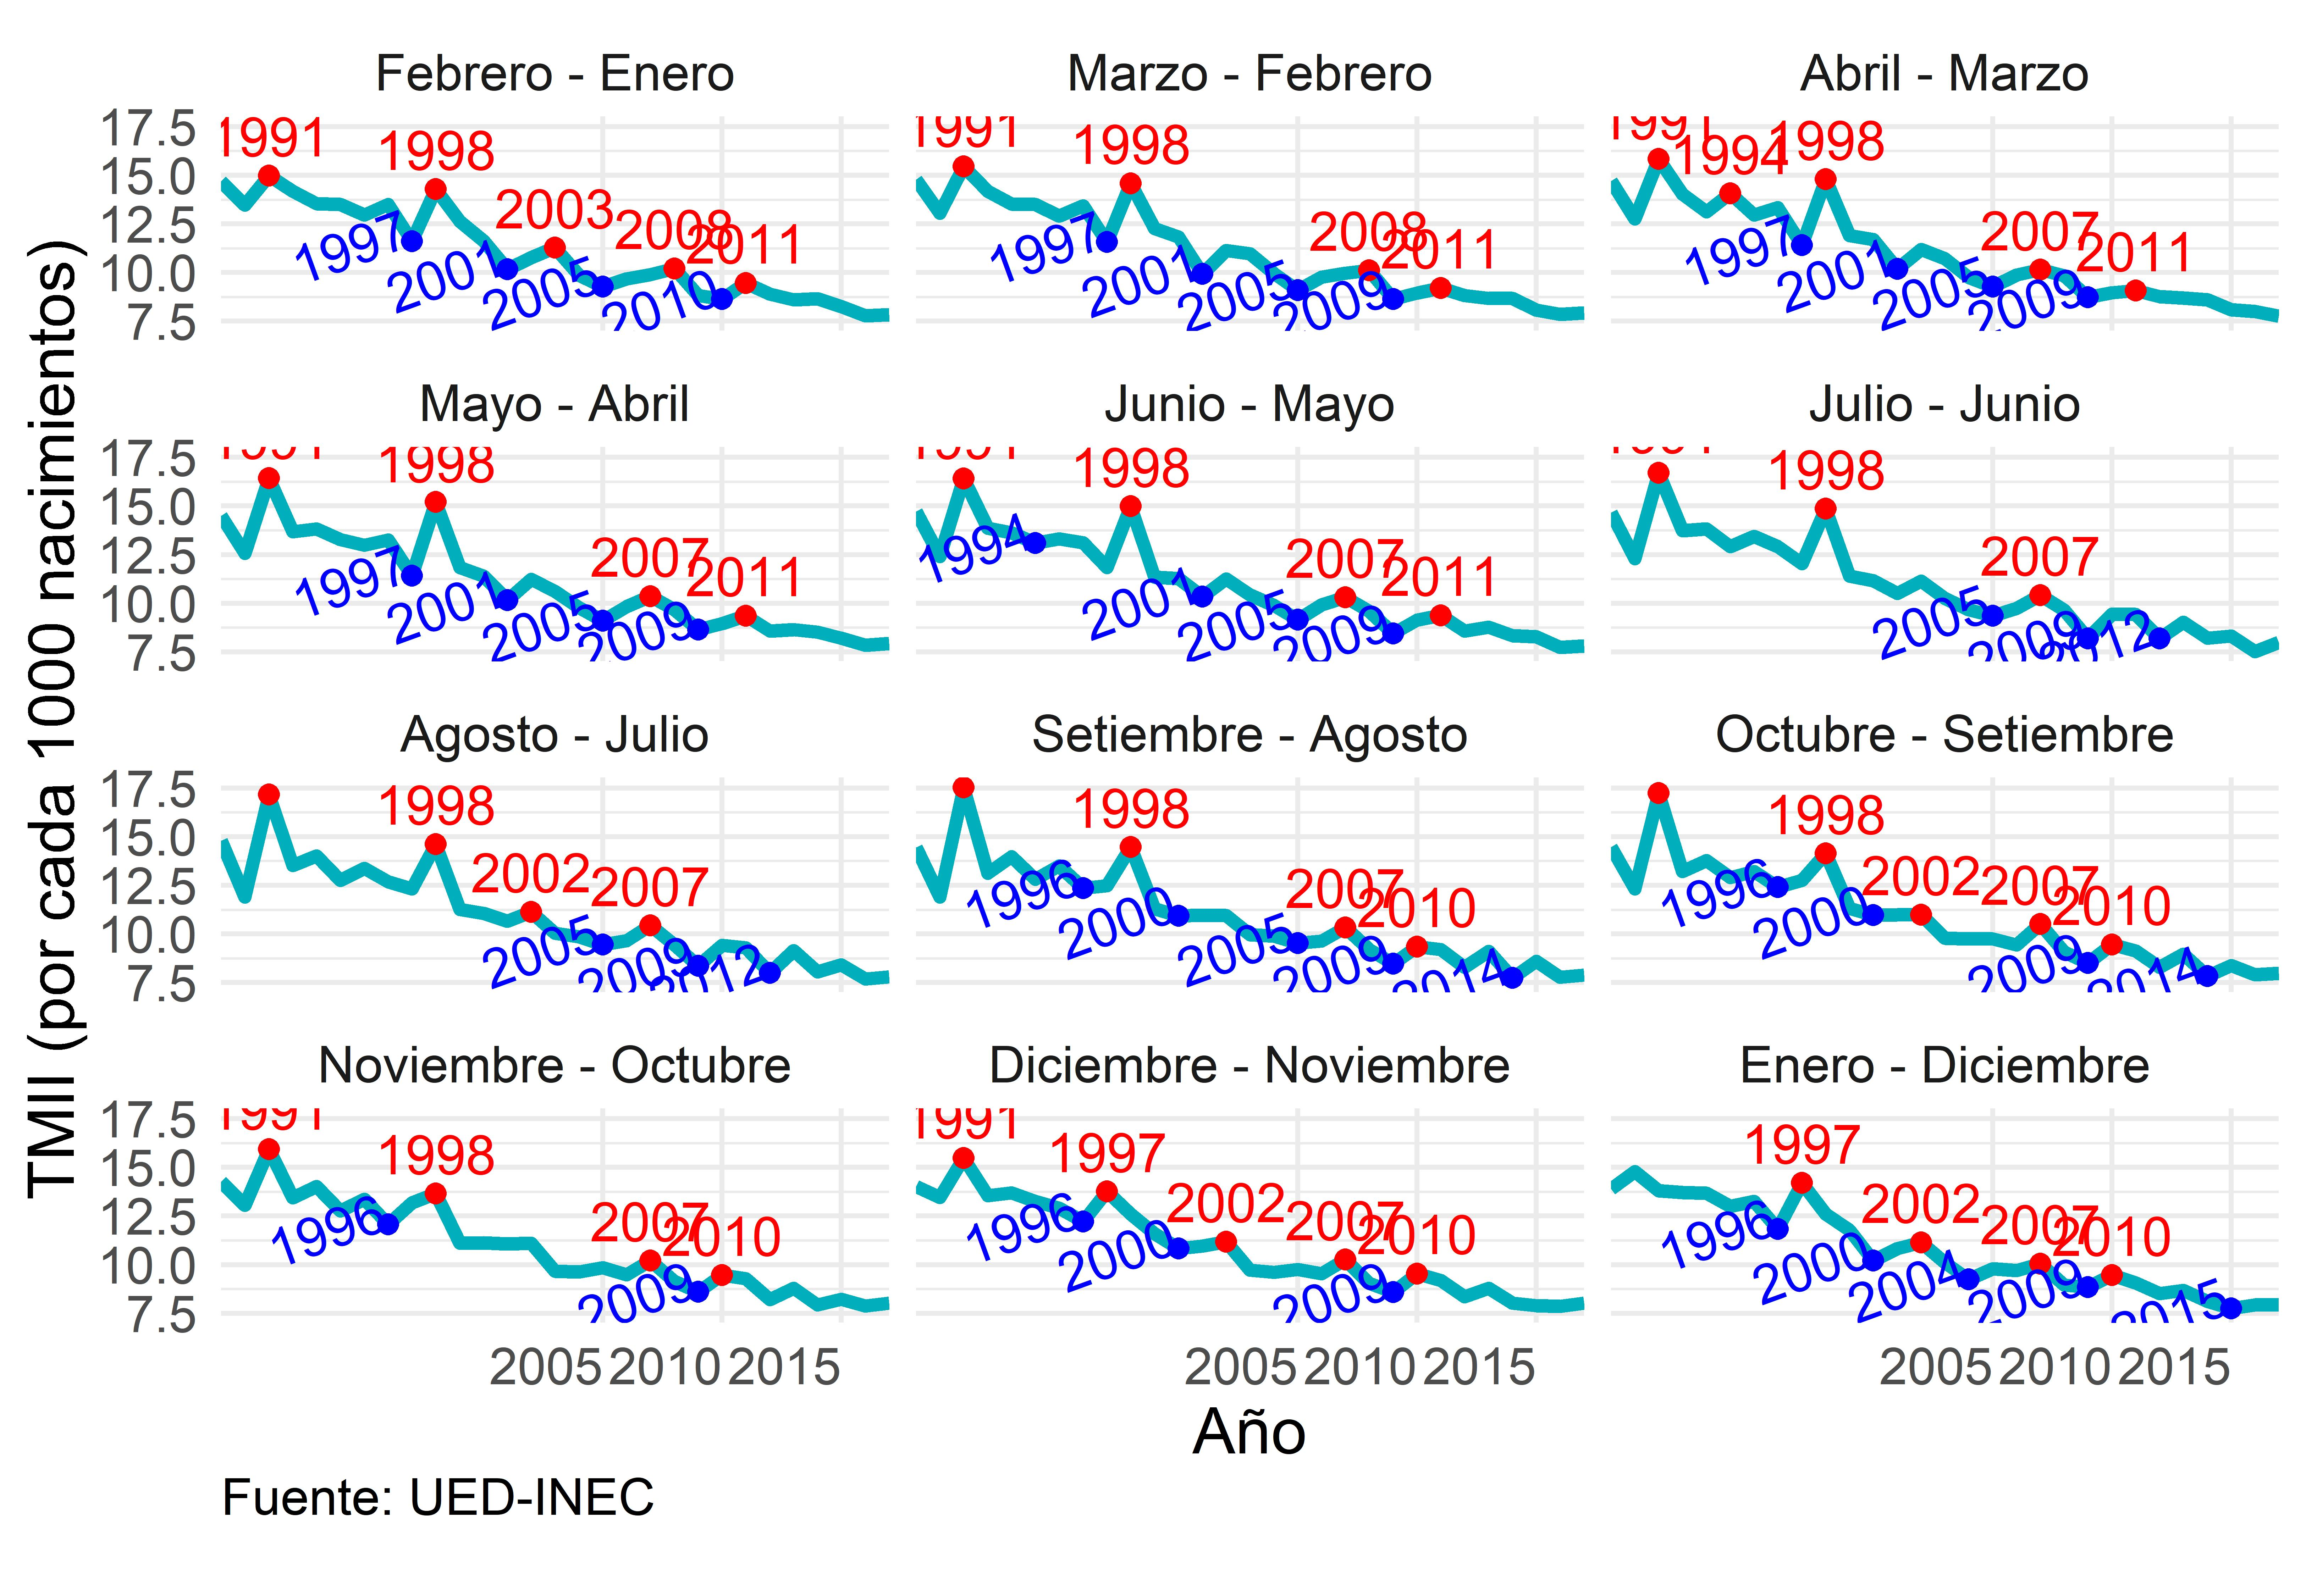
\includegraphics[width=1\linewidth,height=1\textheight]{Tesis_files/figure-latex/tmiiplotperiodos-1} \caption{Tasa de Mortalidad Infantil Interanual 1989 - 2017 según periodos}\label{fig:tmiiplotperiodos}
\end{figure}

Para hacer la descomposición de la serie se hizo una transformación de
Box-Cox con \(\lambda=1\) para aplicarla de manera multiplicativa. Esto
se debe a que en la Figura \ref{fig:tmiiplotgeneral} pueden observarse
cambios considerables en la variabilidad de la serie a lo largo del
tiempo. la Figura \ref{fig:tmiiplotdescomposicion} muestra, como se
mencionó previamente, una tendencia decreciente y una estacionalidad que
no es reiterada a lo largo del tiempo. Además, el componente aleatorio
muestra como los errores no son constantes durante todo el período.

\begin{figure}[H]
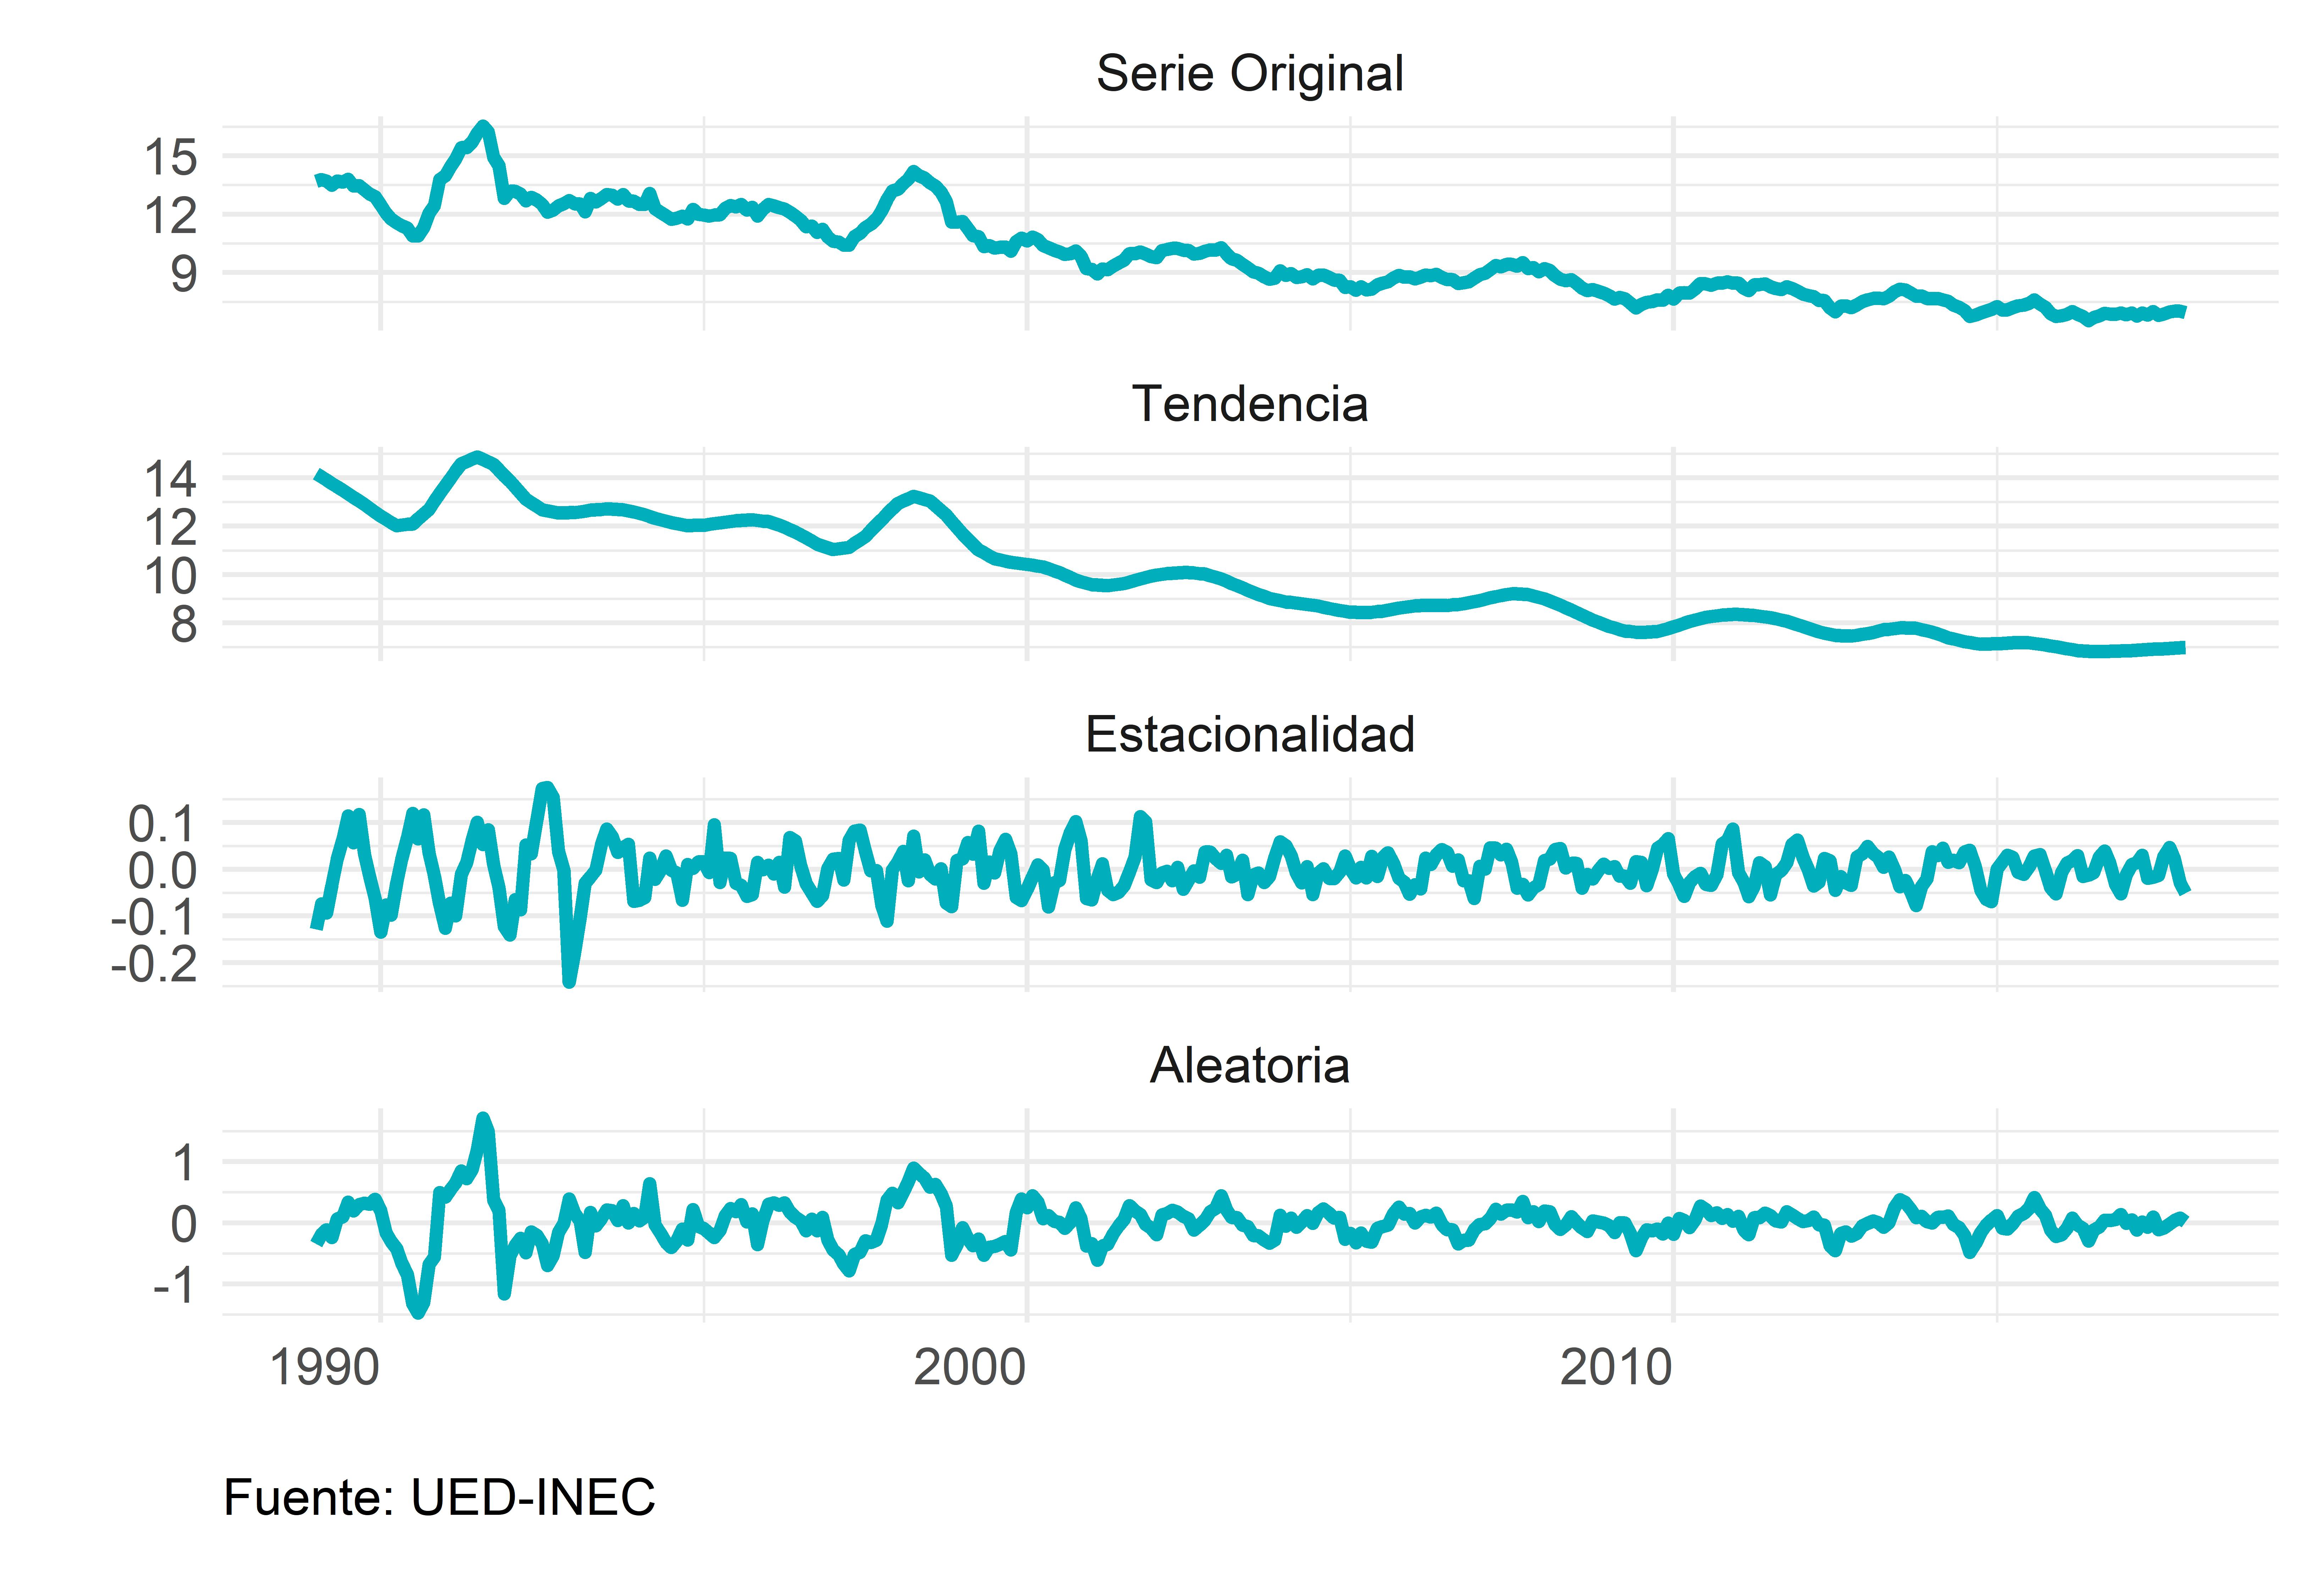
\includegraphics[width=1\linewidth,height=1\textheight]{Tesis_files/figure-latex/tmiiplotdescomposicion-1} \caption{Descomposición de la TMII en el periodo 2000 - 2017}\label{fig:tmiiplotdescomposicion}
\end{figure}

\subsubsection{Mortalidad por causa externa}

La violencia es un acto tan antiguo como el mundo, sin embargo, la
evolución de esta en conjunto con el crecimiento de su relación con las
defunciones registradas en una población la vuelven un problema de salud
pública. En base a la clasificación Internacional de Enfermedades
(\protect\hyperlink{ref-CIE10}{OPS, 2016}) de la de la Organización
Mundial de la Salud\footnote{\url{https://www.paho.org/salud-en-las-americas-2017/?lang=es}{]}},
las defunciones pueden clasificarse en cuatro grandes grupos, siendo el
más importante el de las causas naturales, el cual incluye enfermedades
congénitas, cardiopatías u otras relacionadas con la vejez. En menor
cuantía se encuentran las causas de muerte ignoradas, las cuales se dan
cuando la causa de muerte es desconocida y de intención indeterminada; y
de forma similar se encuentran las causas de muerte que se mantienen en
estudio, bien sea por parte de la morgue o de algún otro organismo, esta
última tiene pocos registros conforme más se retrocede en el tiempo.

El otro gran grupo, aunque considerablemente menor que las causas
naturales, son las causas externas, las cuales son objeto de análisis en
este apartado. Este grupo puede a su vez ser clasificado en homicidios,
suicidios y las muertes accidentales, esta última comprende los
accidentes de tránsito, las muertes por caídas, personas ahogadas,
víctimas de incendios, terraplenes u otros similares. Aunado a estas
categorías se encuentran también las causas indeterminadas, las cuales
se diferencian a las ignoradas en que se sabe que se debe a una causa
externa pero no se conoce con certeza a cuál categoría pertenece o aún
está en investigación, tal es el caso de una persona que fallece debido
a una alta ingesta de drogas o estupefacientes; bien pudo haber
consumido intencionalmente hasta morir, lo cual sería un suicidio, o
bien el consumo excesivo se debió a un accidente.

En Costa Rica para el año 2011, las muertes por causas externas ocuparon
el tercer lugar, siendo solo superadas por las enfermedades del sistema
circulatorio, en particular las enfermedades cardiovasculares, y los
tumores, ambos casos mostraron una tendencia ascendente
(\protect\hyperlink{ref-nacion}{INEC, 2013}). Es debido a los elevados
costos económicos y sociales
(\protect\hyperlink{ref-ccpexternas}{Cardona, 2013}) que se aborda la
imperiosa necesidad comprender el comportamiento de las defunciones
debido a las causas externas con el fin de contar con un punto de
partida para la elaboración de políticas públicas que busquen reducir al
mínimo este tipo de eventos.

Dado que los registros de defunciones por causa externa se realizan
diariamente, conviene analizar su comportamiento de manera mensual desde
inicios del milenio de una manera más general, dicho comportamiento
puede observarse en la Figura \ref{fig:externaplotgeneral}.

\begin{figure}[H]
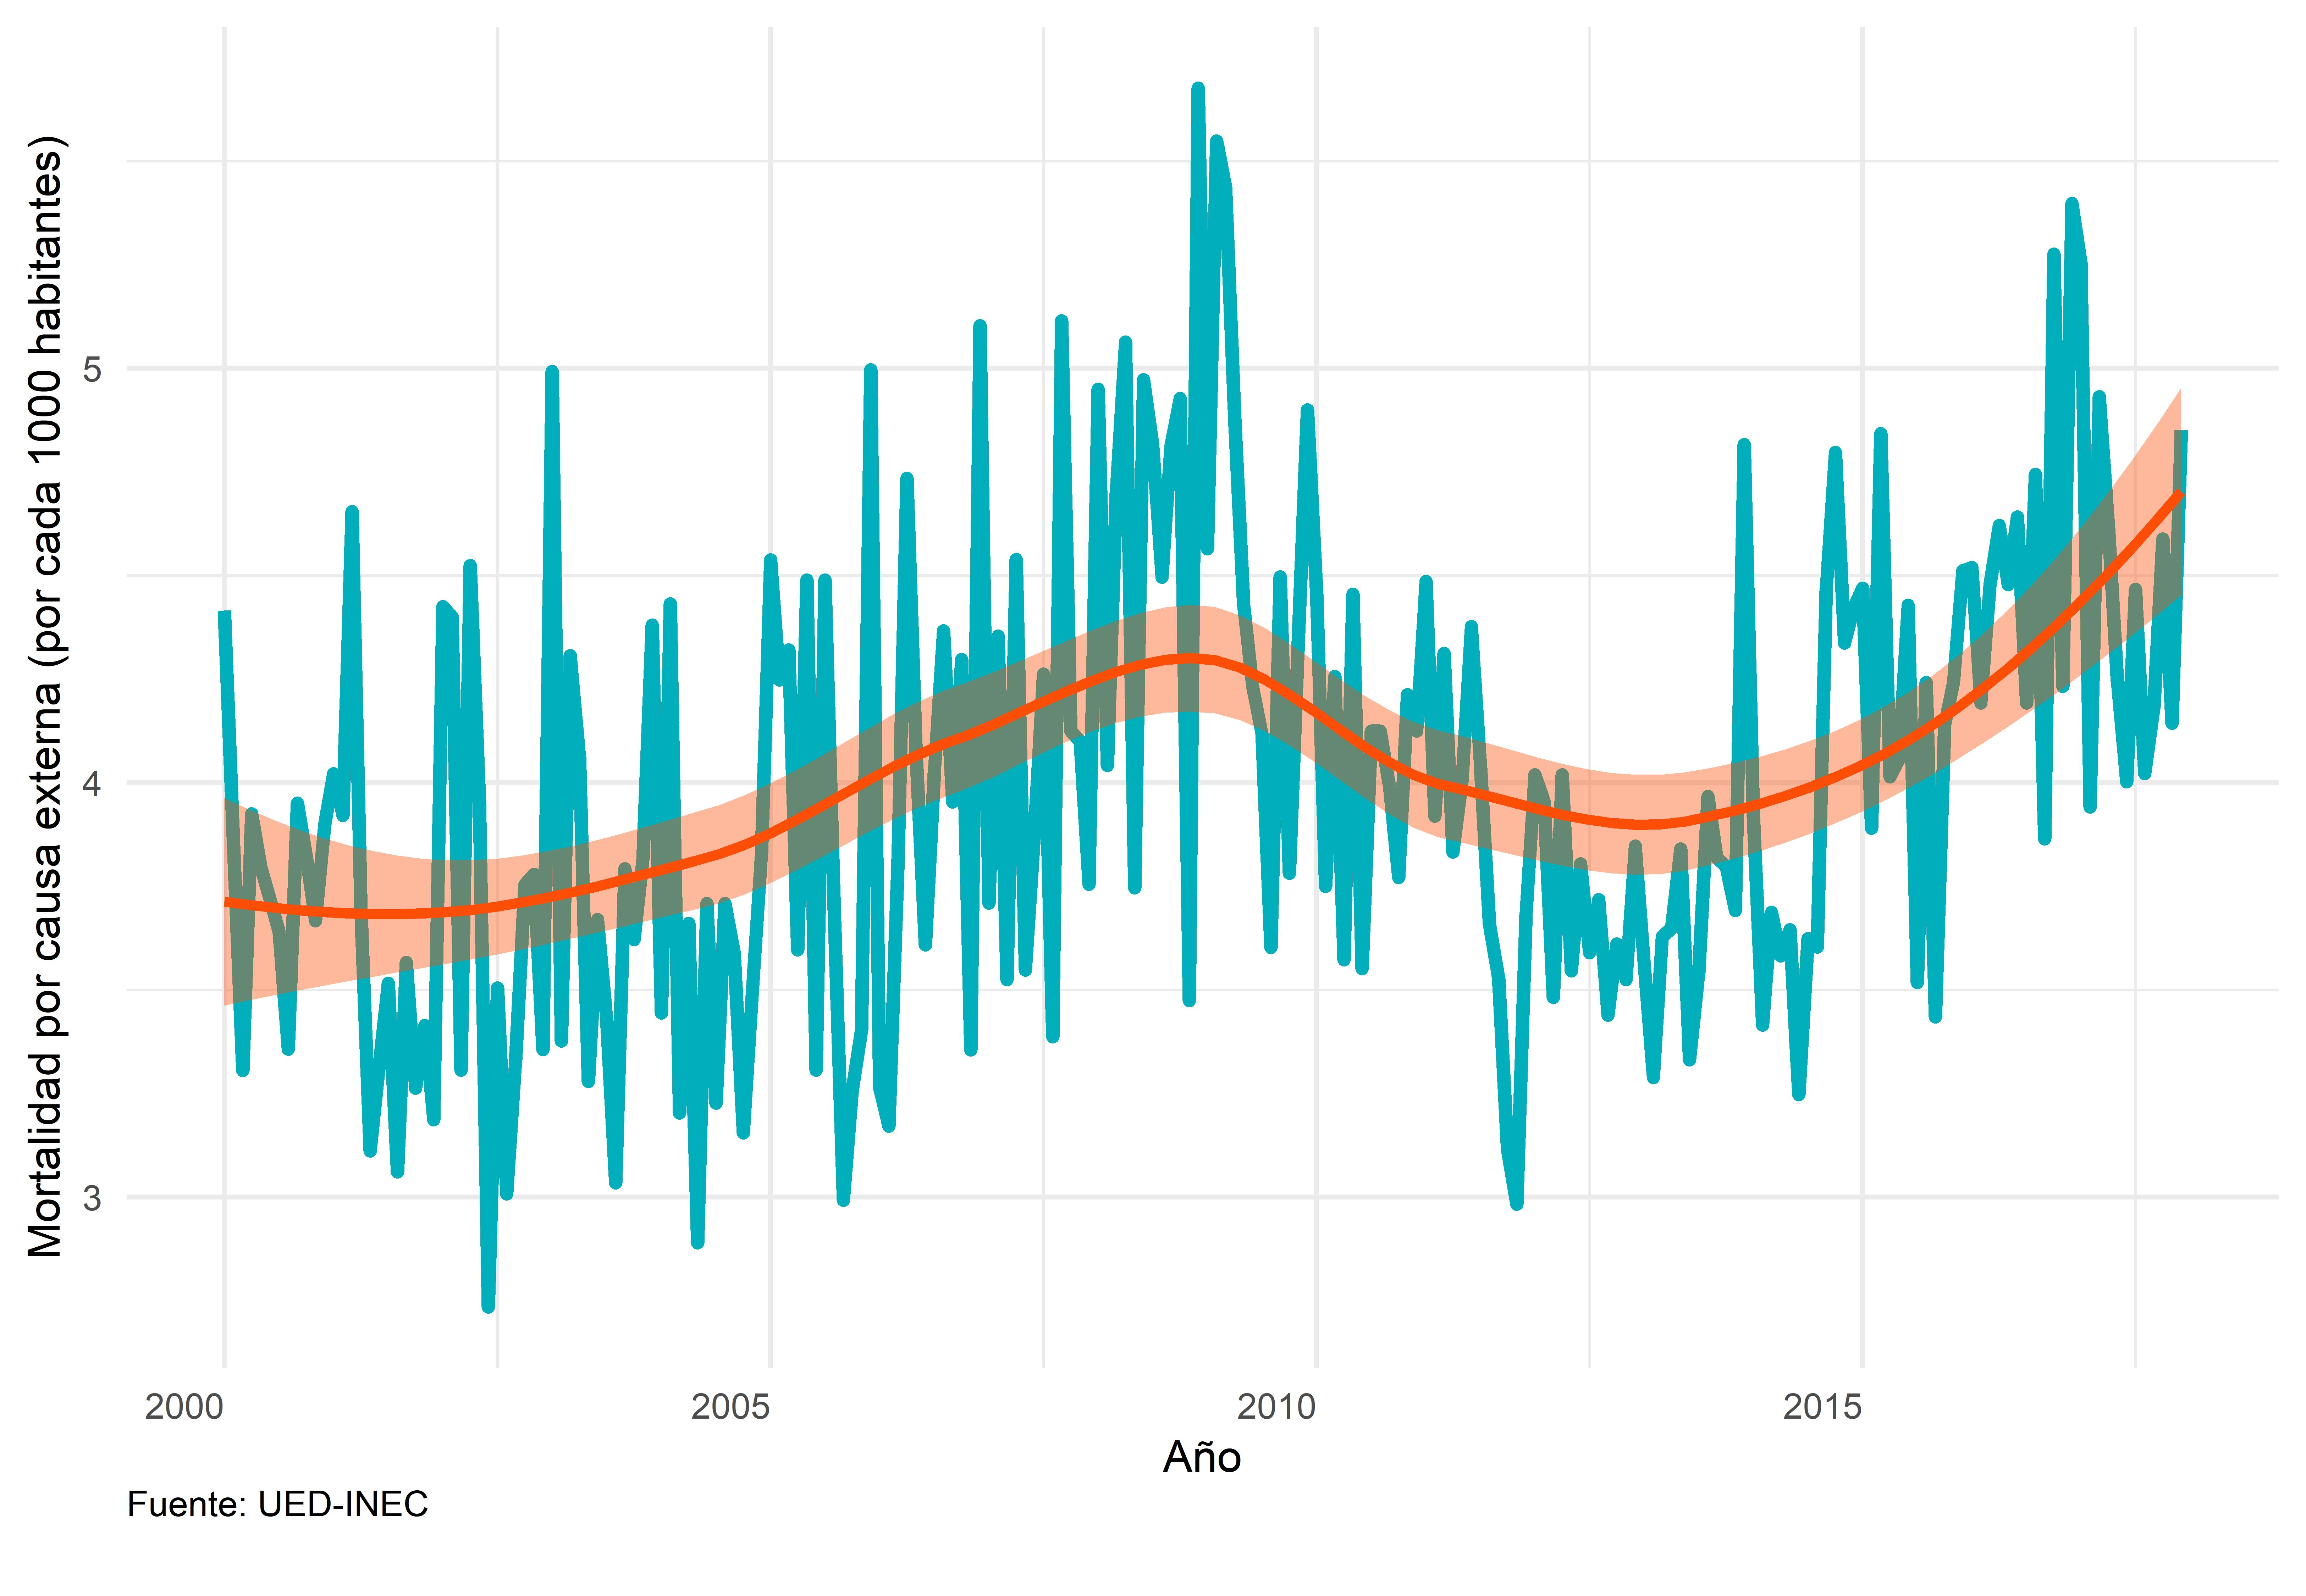
\includegraphics[width=1\linewidth,height=1\textheight]{Tesis_files/figure-latex/externaplotgeneral-1} \caption{Mortalidad por causa externa 2000 - 2017}\label{fig:externaplotgeneral}
\end{figure}

Es importante recalcar que, entre Junio del año 2012 y Diciembre del año
2017, el aumento en la tasa de cambio de la cantidad de defunciones
debido a causas externas coincide con el aumento de la flotilla de
motocicletas, pues en un período de cinco años esta cifra creció en un
189\% (\protect\hyperlink{ref-motos}{Vázquez, 2017}). Conviene entonces
verificar el comportamiento a lo interno de la serie en referencias a
las categorías de las causas externas.

De la Figura \ref{fig:externasplotperiodos} puede notarse que cada mes
tiene sus picos y valles durante cada mes a lo largo del periodo, siendo
los meses de Enero, Abril y Diciembre los que presentaron valores
ligeramente más altos entre los años 2000 y 2017.

\begin{figure}[H]
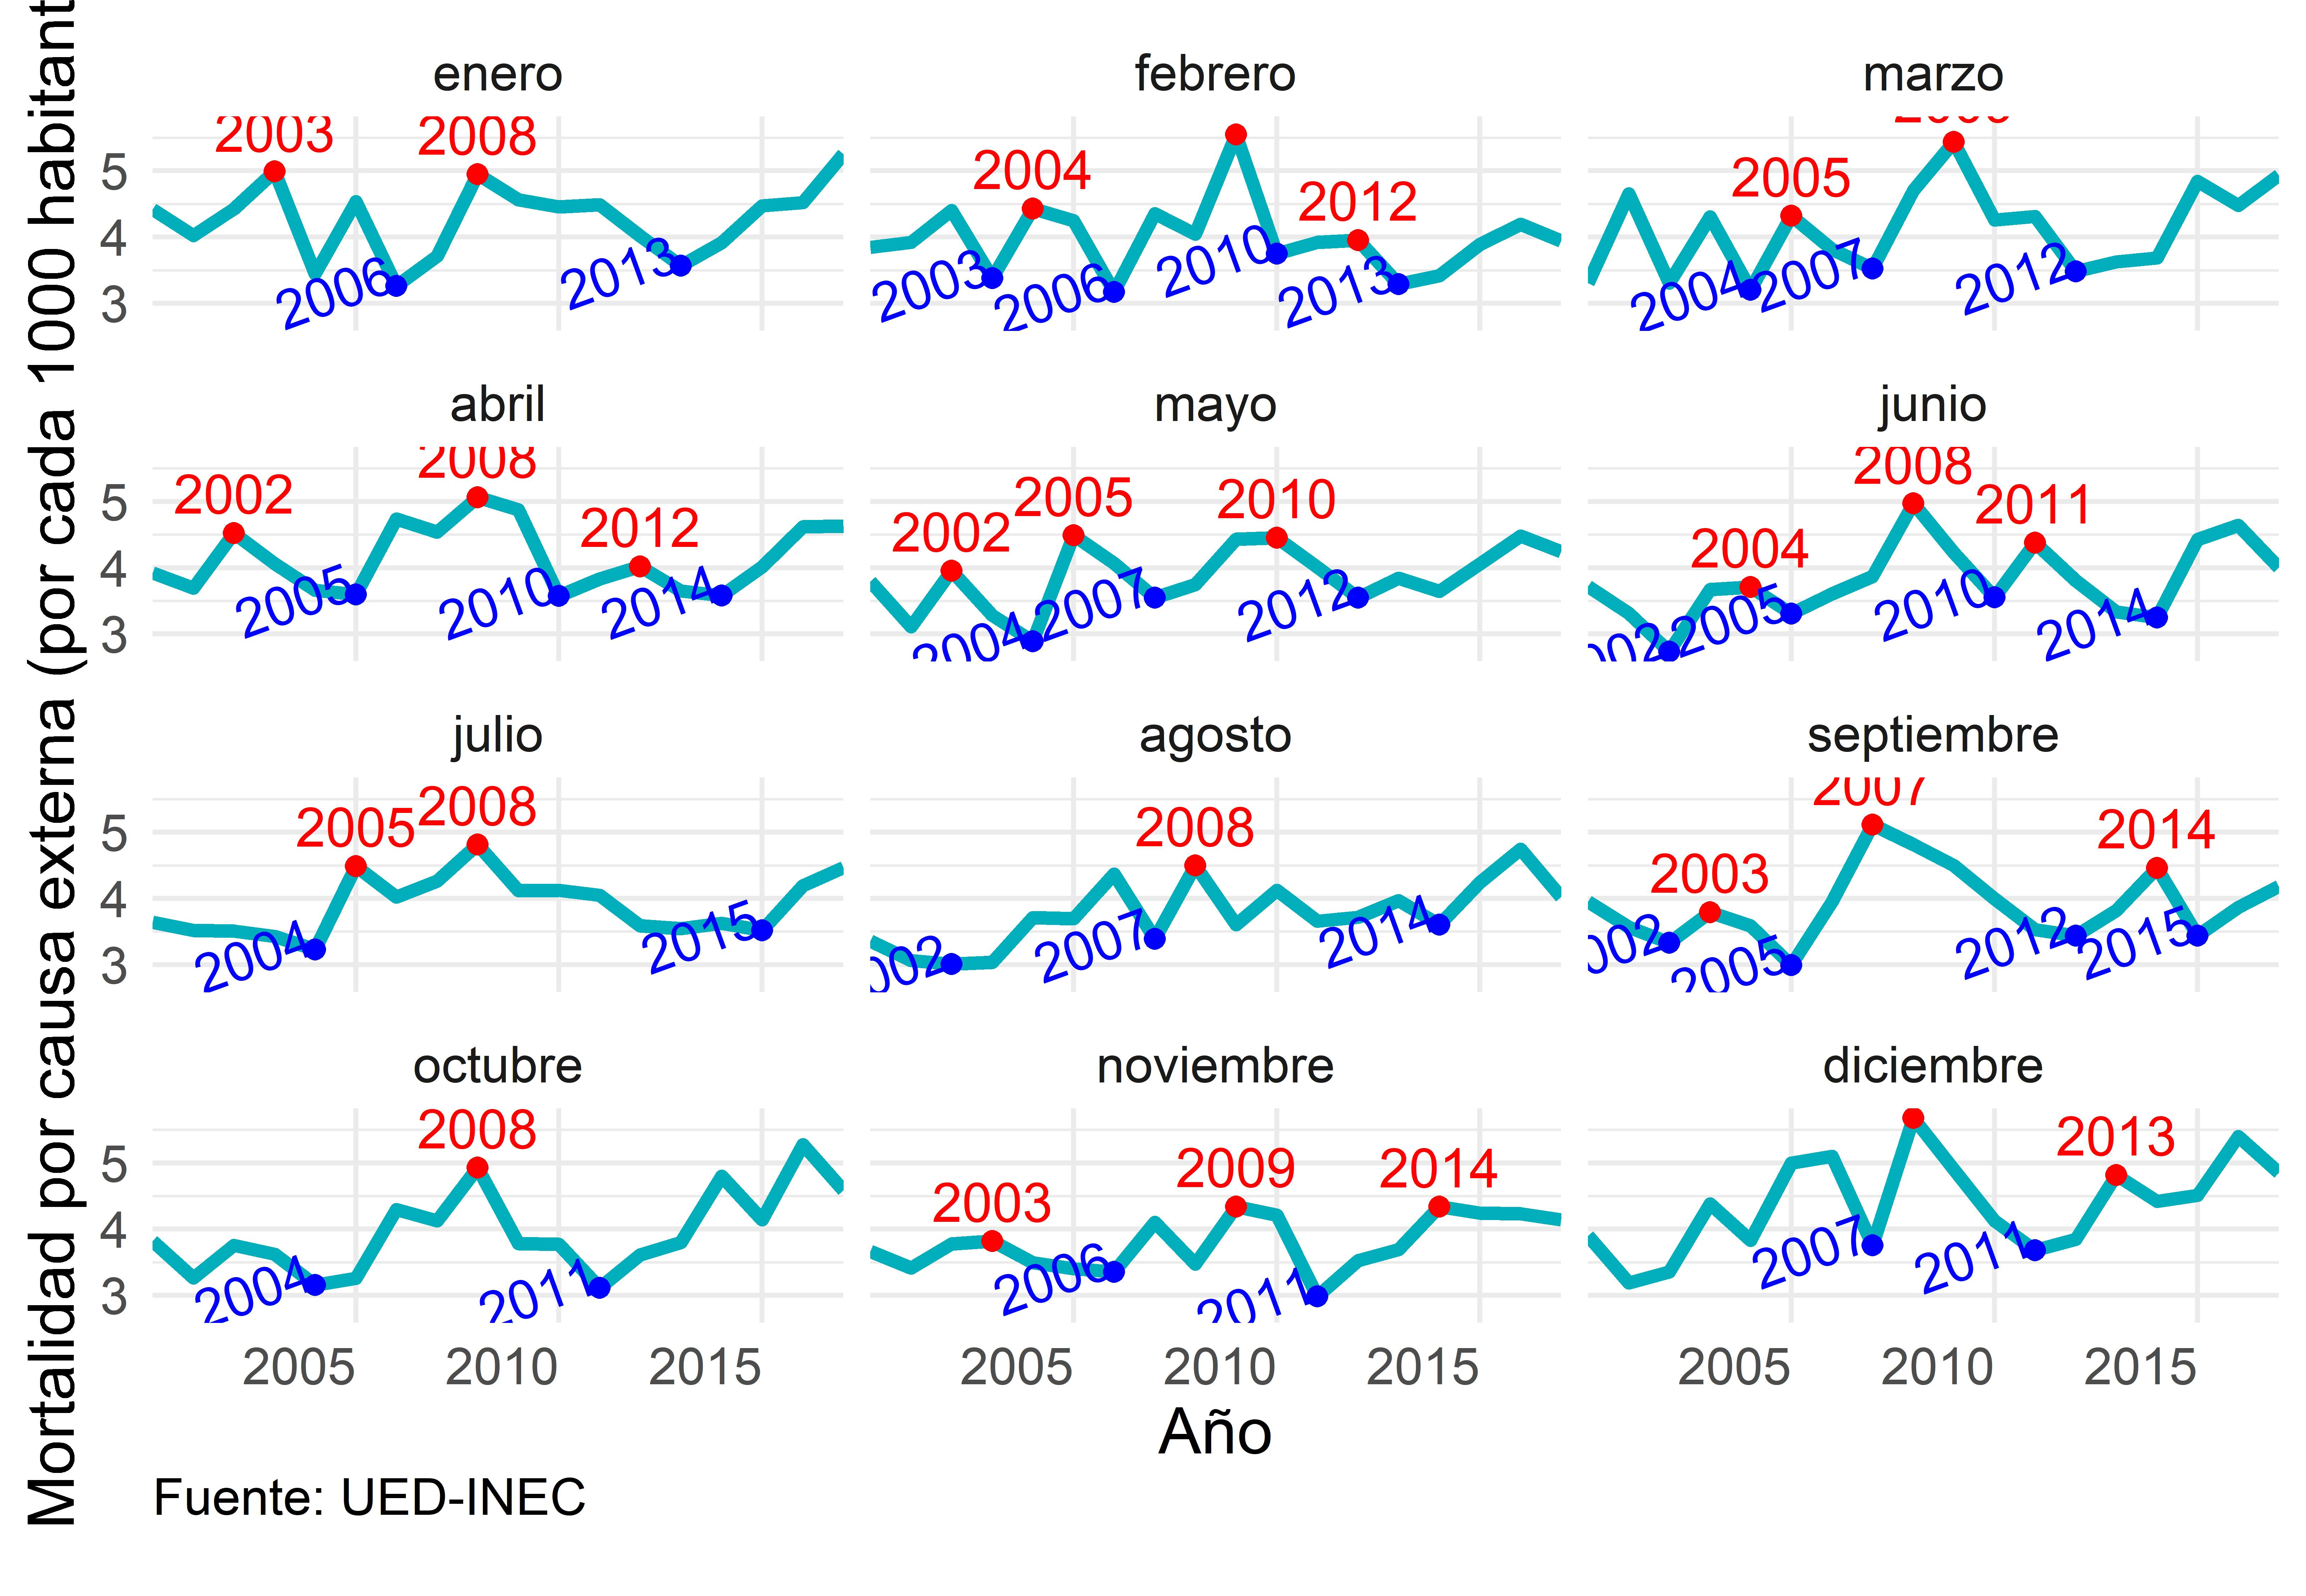
\includegraphics[width=1\linewidth,height=1\textheight]{Tesis_files/figure-latex/externasplotperiodos-1} \caption{Mortalidad por causa externa 2000 - 2017 según mes}\label{fig:externasplotperiodos}
\end{figure}

La descomposición de la serie se hará de forma aditiva debido a que en
el gráfico 1 no se observan grandes cambios en la variabilidad a lo
largo del tiempo. La Figura \ref{fig:externasplotdescomposicion} muestra
que la tendencia se mantiene casi constante a lo largo del tiempo,
mientras que parece haber estacionalidad en ciertos lapsos de la segunda
mitad del año. Además, el componente aleatorio muestra como los errores
no son constantes a lo largo de todo el período.

\begin{figure}[H]
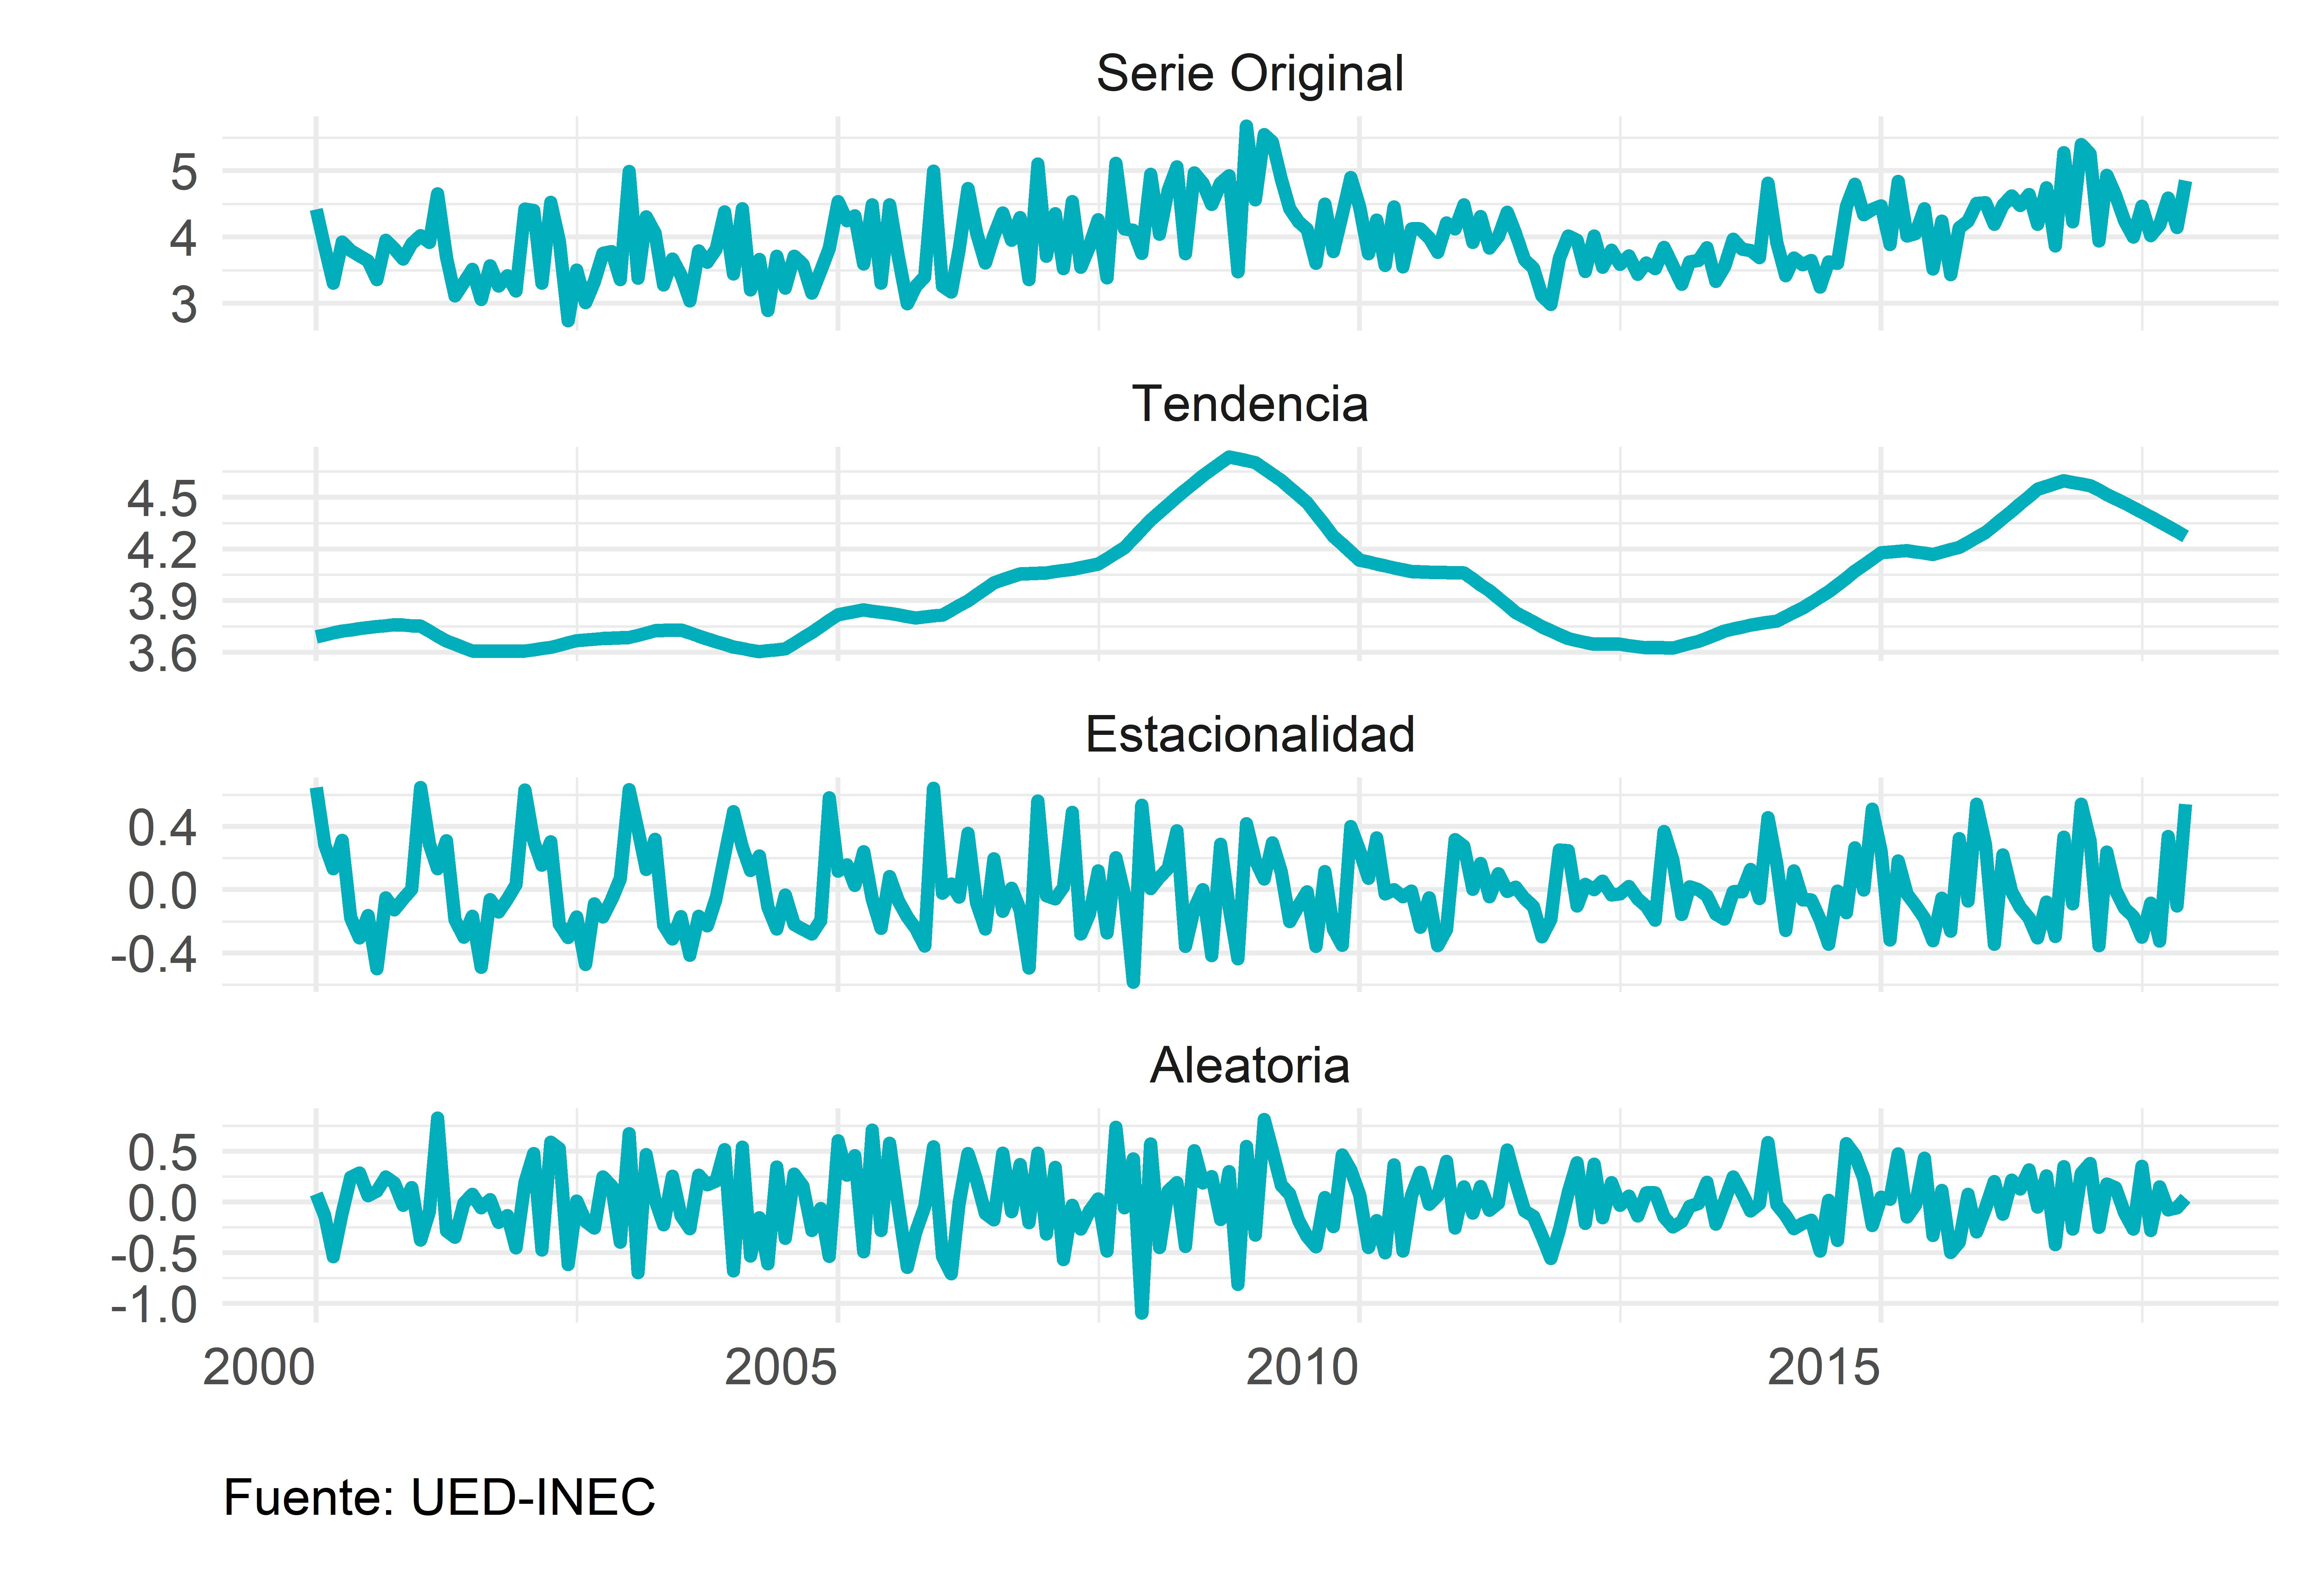
\includegraphics[width=1\linewidth,height=1\textheight]{Tesis_files/figure-latex/externasplotdescomposicion-1} \caption{Descomposición de las defunciones por causa externa en el periodo 2000-2017}\label{fig:externasplotdescomposicion}
\end{figure}

\subsubsection{Incentivos salariales del sector público}

Los incentivos salariales son retribuciones que de conformidad con la
legislación vigente se asignan al servidor por sus características
laborales que complementan las remuneraciones básicas. Los incentivos se
reconocen tanto a profesionales como a no profesionales, facultados por
disposiciones jurídicas que así lo autorizan. Algunos de estos
incentivos son: anualidades, dedicación exclusiva, salario escolar,
carrera profesional, carrera técnica, zonaje, desarraigo,
regionalización, riesgo policial, riesgo penitenciario, riesgo de
seguridad y vigilancia, peligrosidad, incentivo didáctico, entre otros.
Esta serie cronológica representa los incentivos salariales en millones
de colones del sector público de Costa Rica de enero 2007 a junio 2015.

De manera análoga a las secciones anteriores, la Figura
\ref{fig:incentivosplotgeneral} muestra el comportamiento general de la
serie cronológica. al hacer un suavizamiento Loess hay un ligero cambio
de concavidad a partir de Julio 2008, lo cual sugiere que a partir de
este momento los incentivos salariales vuelvan a alcanzar valores
similares a los mostrados al inicio de la serie. La Figura
\ref{fig:incentivosplotperiodos} muestra cómo hay un crecimiento
sostenido de los incentivos en cada mes a lo largo de todo el periodo.
Sin embargo, este crecimiento se da a una tasa mucho mayor en la época
de fin y principio de año.

\begin{figure}[H]
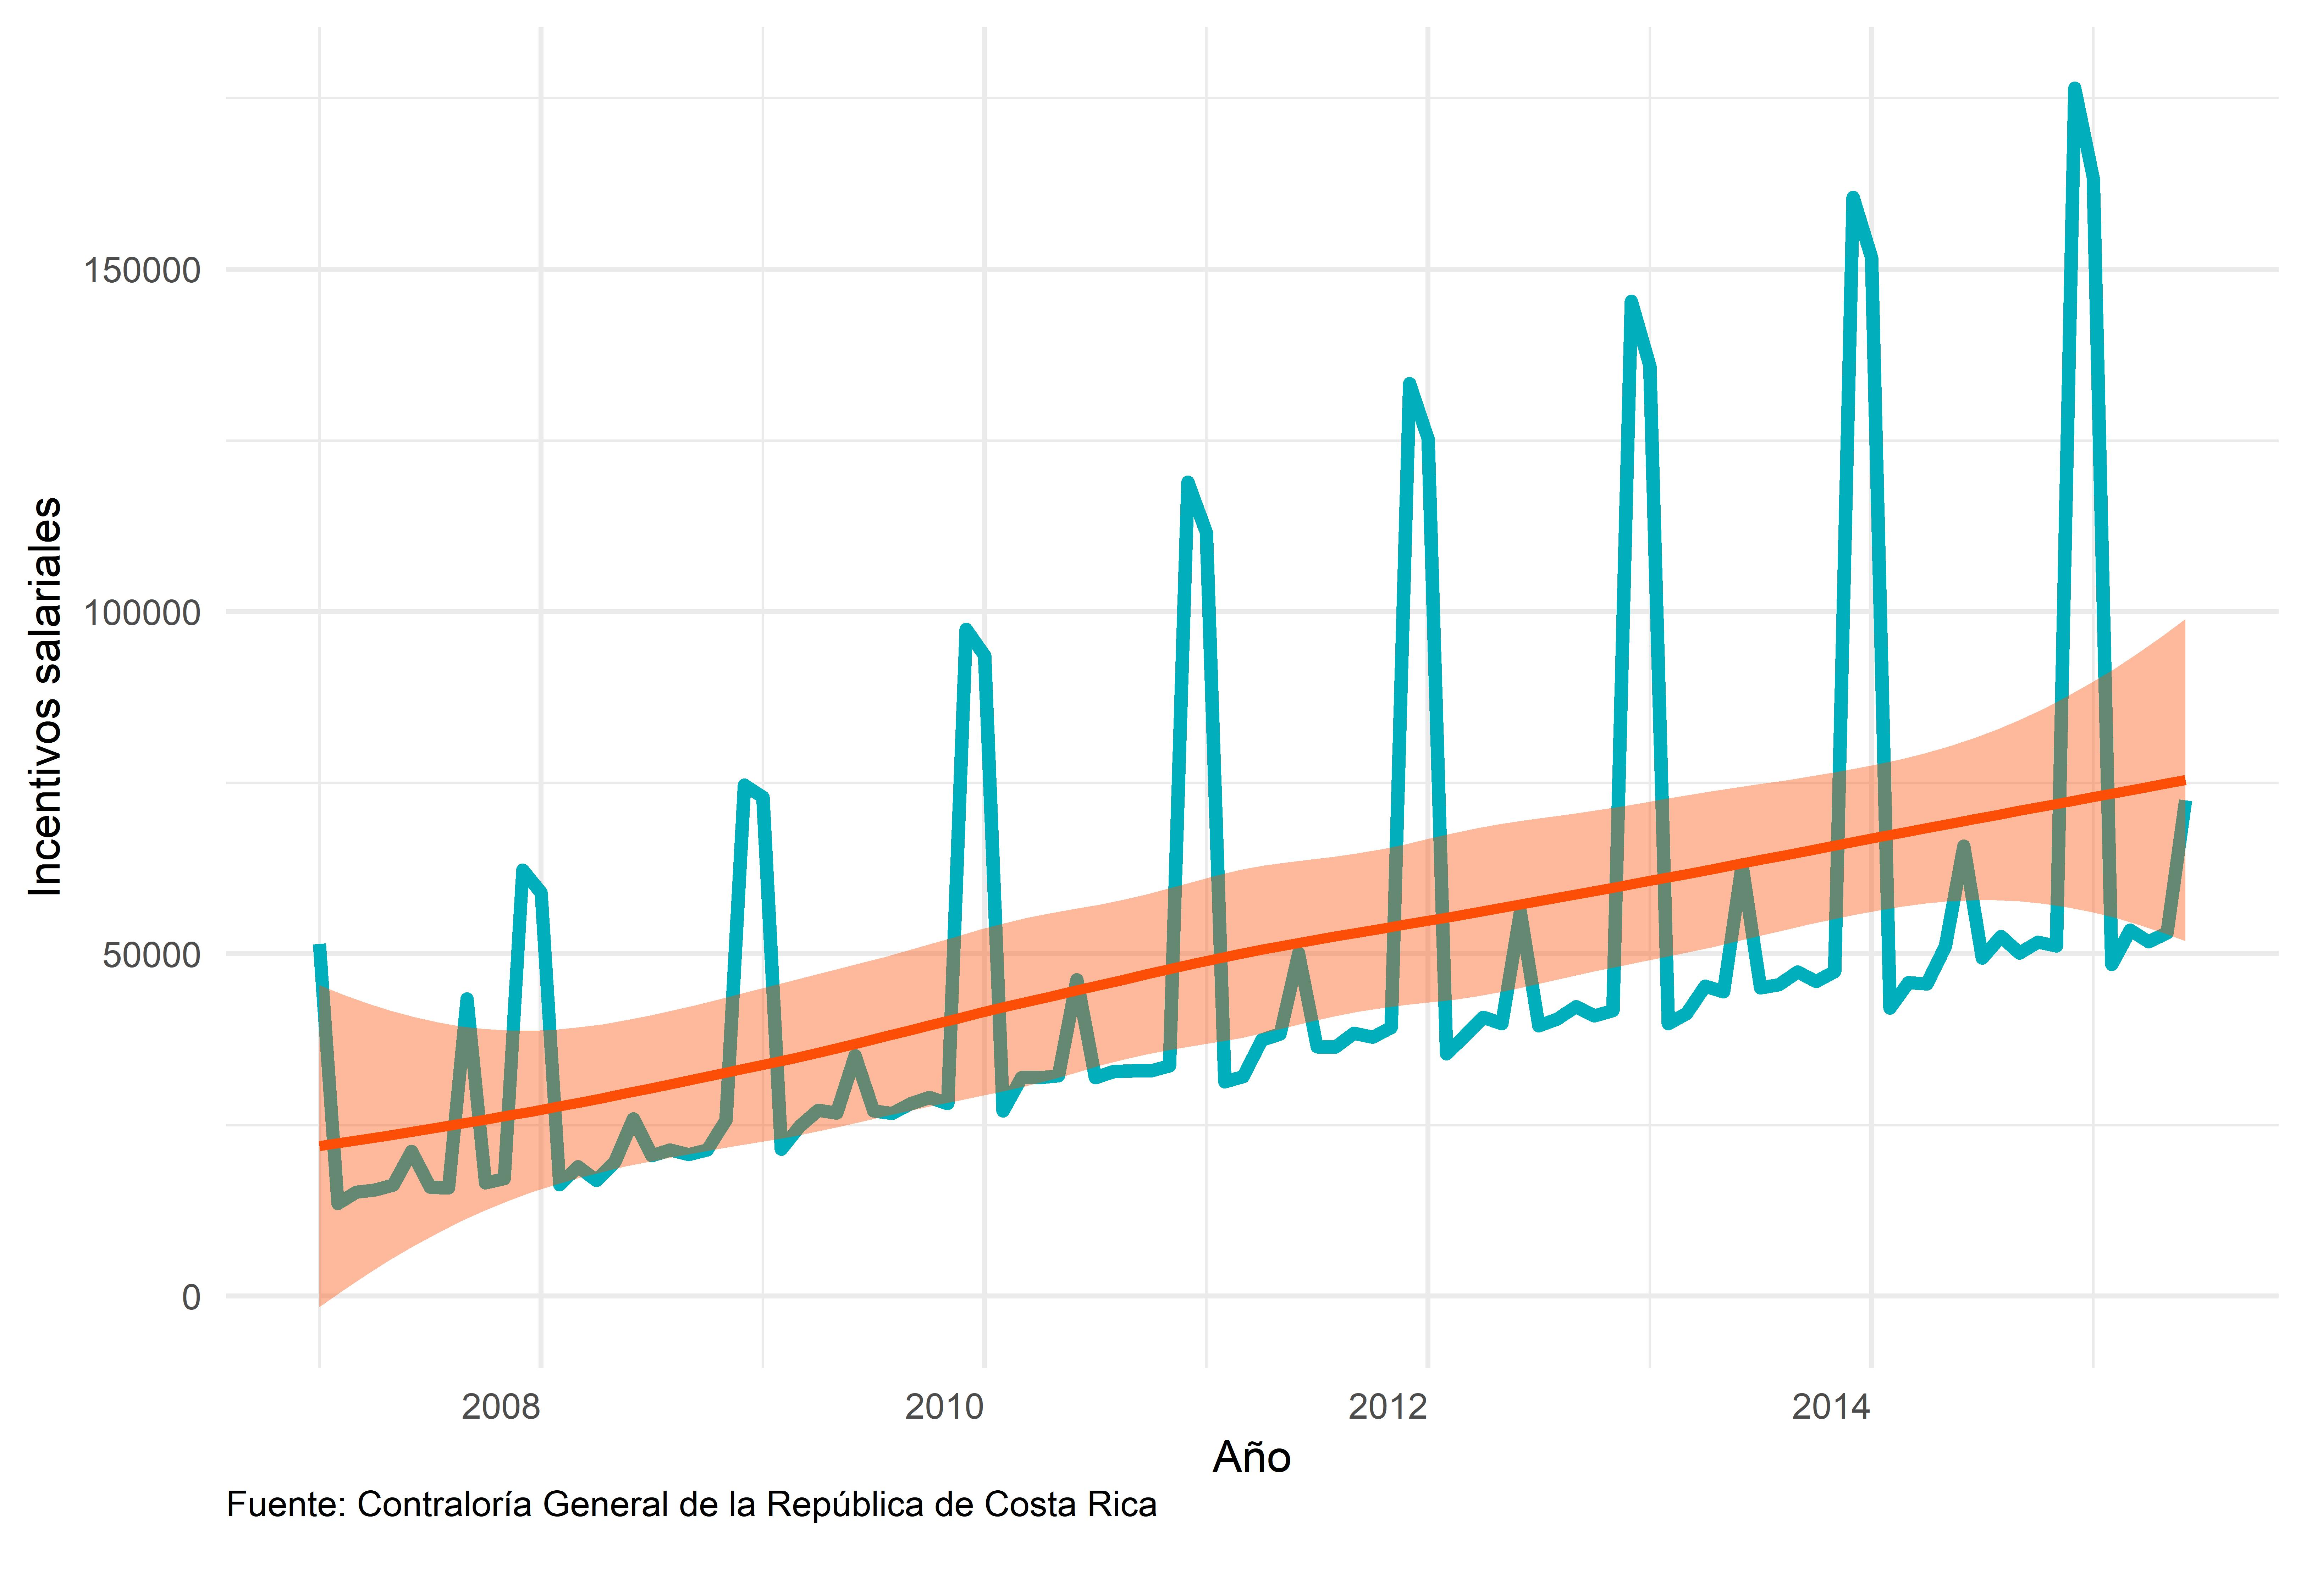
\includegraphics[width=1\linewidth,height=1\textheight]{Tesis_files/figure-latex/incentivosplotgeneral-1} \caption{Incentivos salariales en el sector público 2007 - 2018}\label{fig:incentivosplotgeneral}
\end{figure}

\begin{figure}[H]
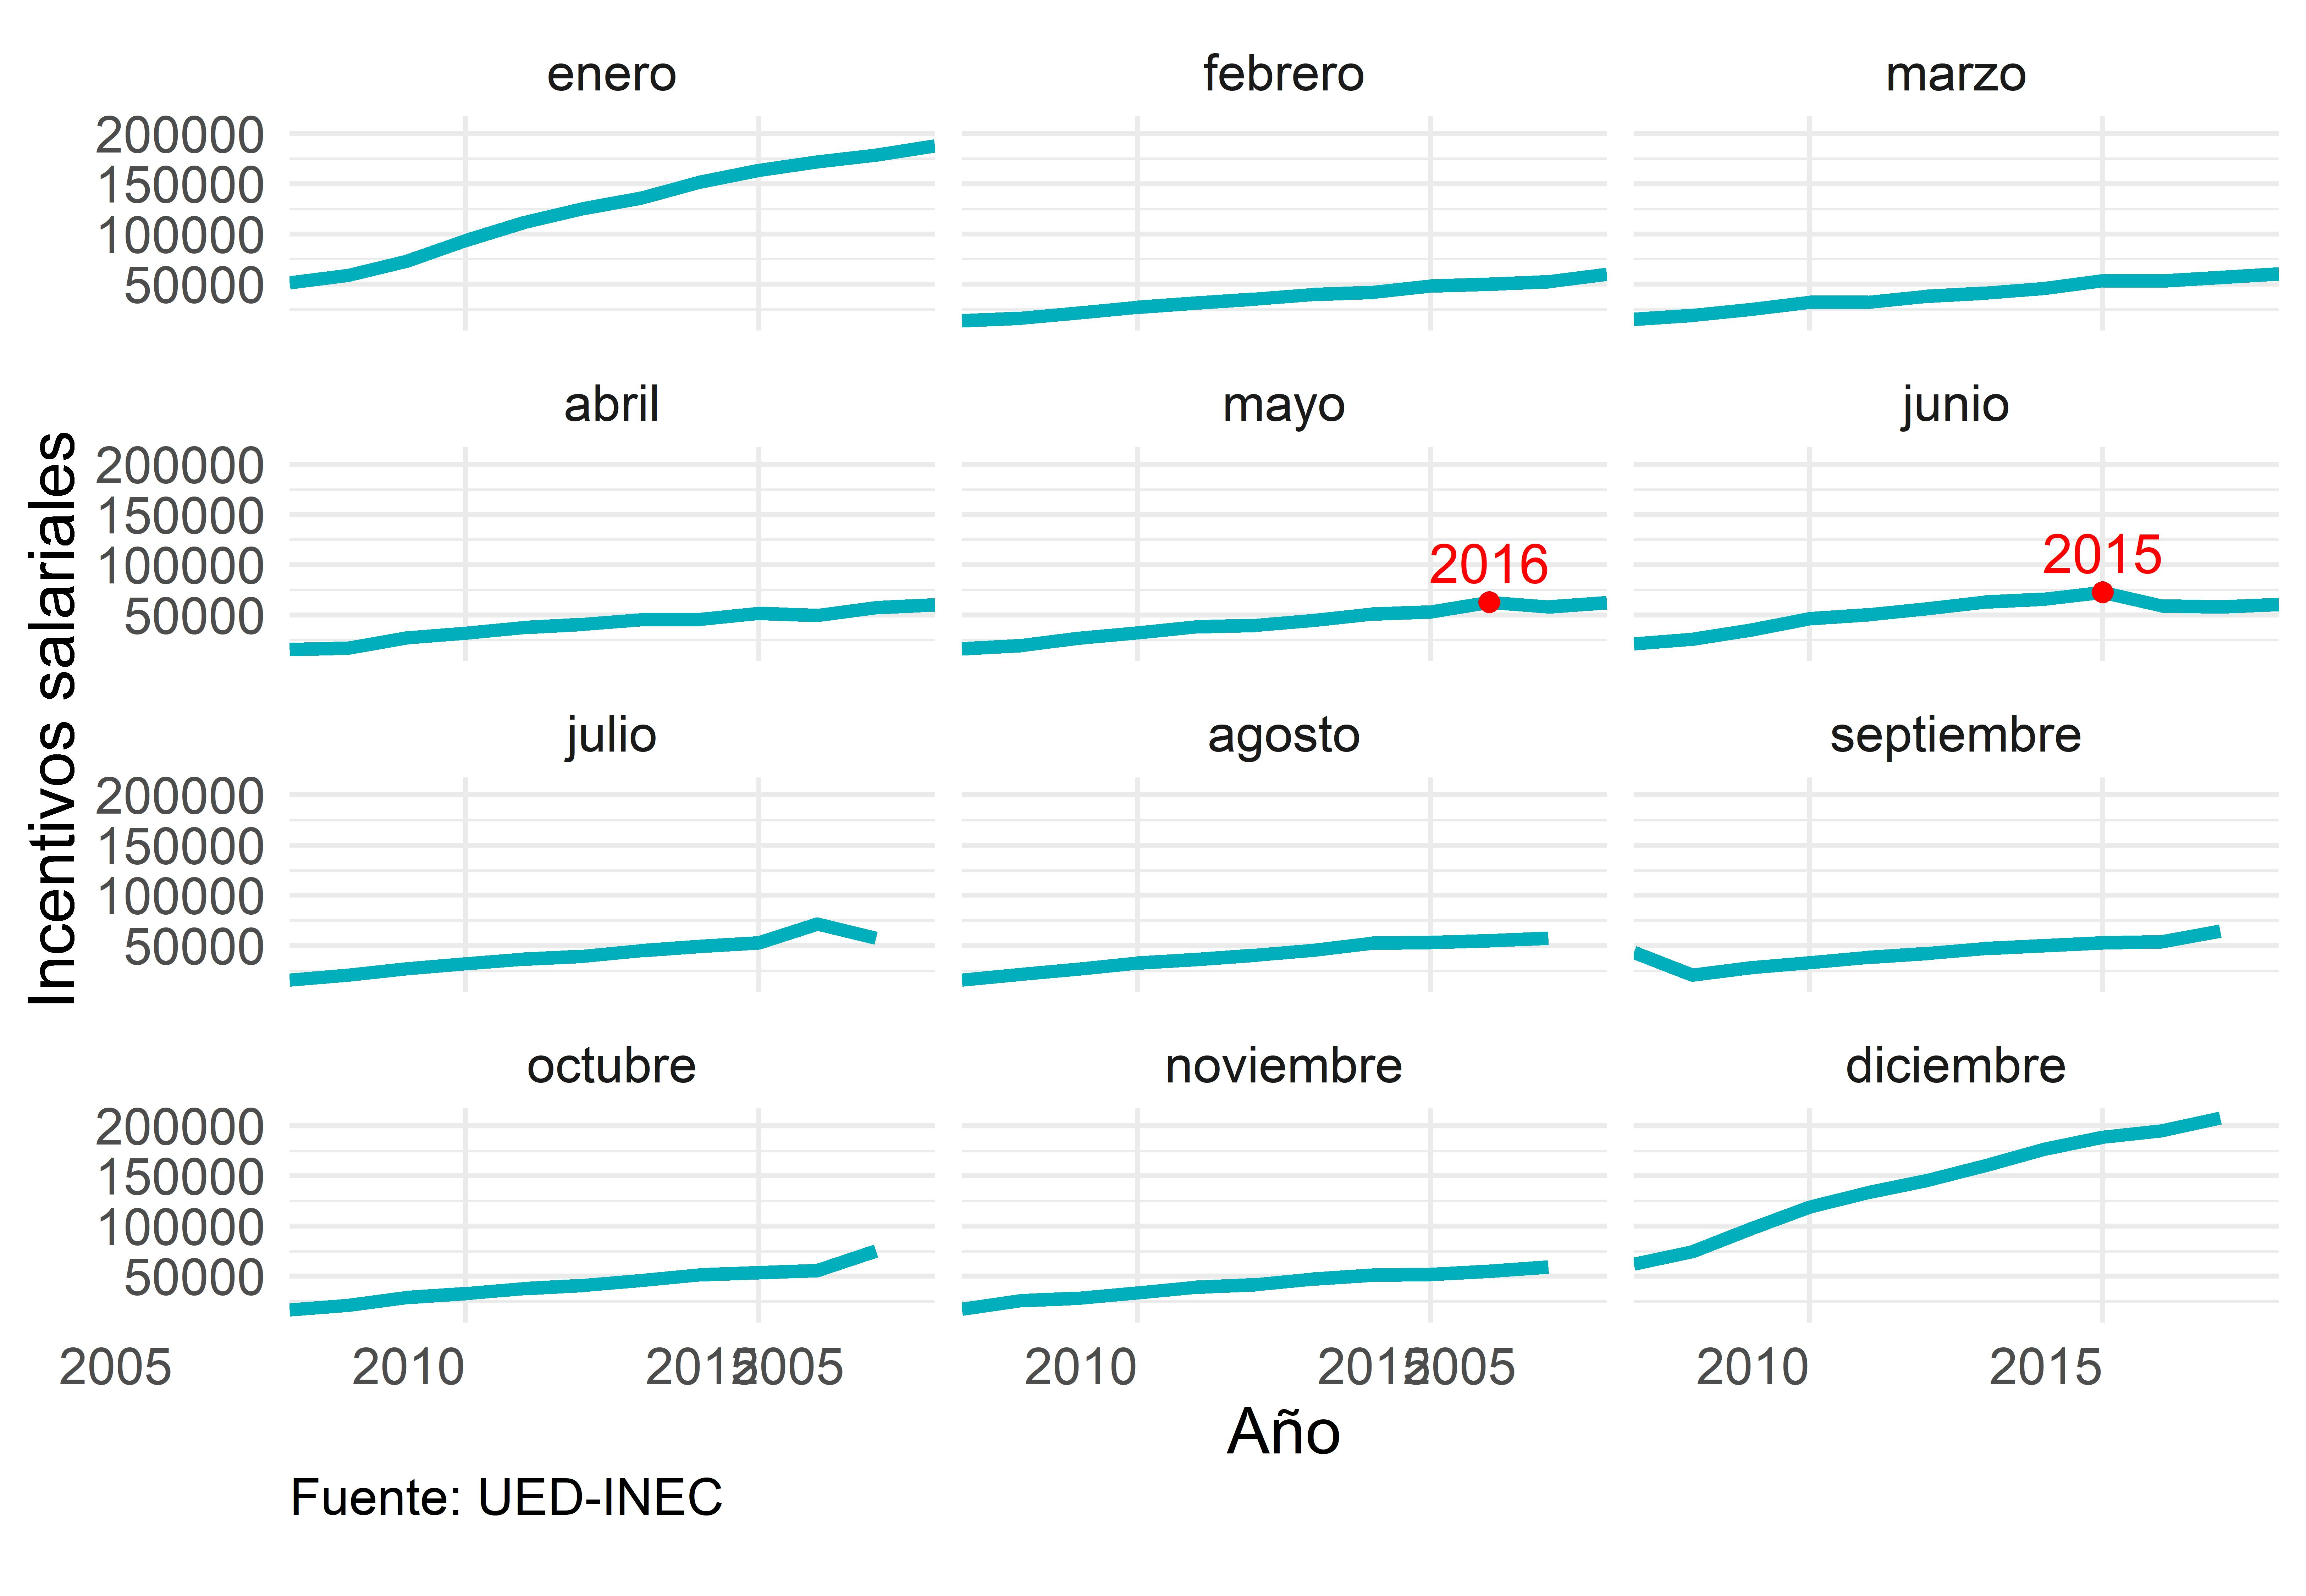
\includegraphics[width=1\linewidth,height=1\textheight]{Tesis_files/figure-latex/incentivosplotperiodos-1} \caption{Incentivos salariales en el sector público 2007 - 2018 según mes}\label{fig:incentivosplotperiodos}
\end{figure}

En la Figura \ref{fig:incentivosplotdescomposicion} se muestra la
descomposición de la serie en sus distintos componentes. Pueden
observarse, además de un crecimiento a lo largo del tiempo, los picos y
las caídas en la parte estacional, esto hace referencia a los meses de
Diciembre y Enero; cuando no se está en este periodo los incentivos
poseen un comportamiento más estable. El componente aleatorio muestra
indicios de que la variabilidad de la serie no es homogénea, sino que
cambia conforme pasa el tiempo.

\begin{figure}[H]
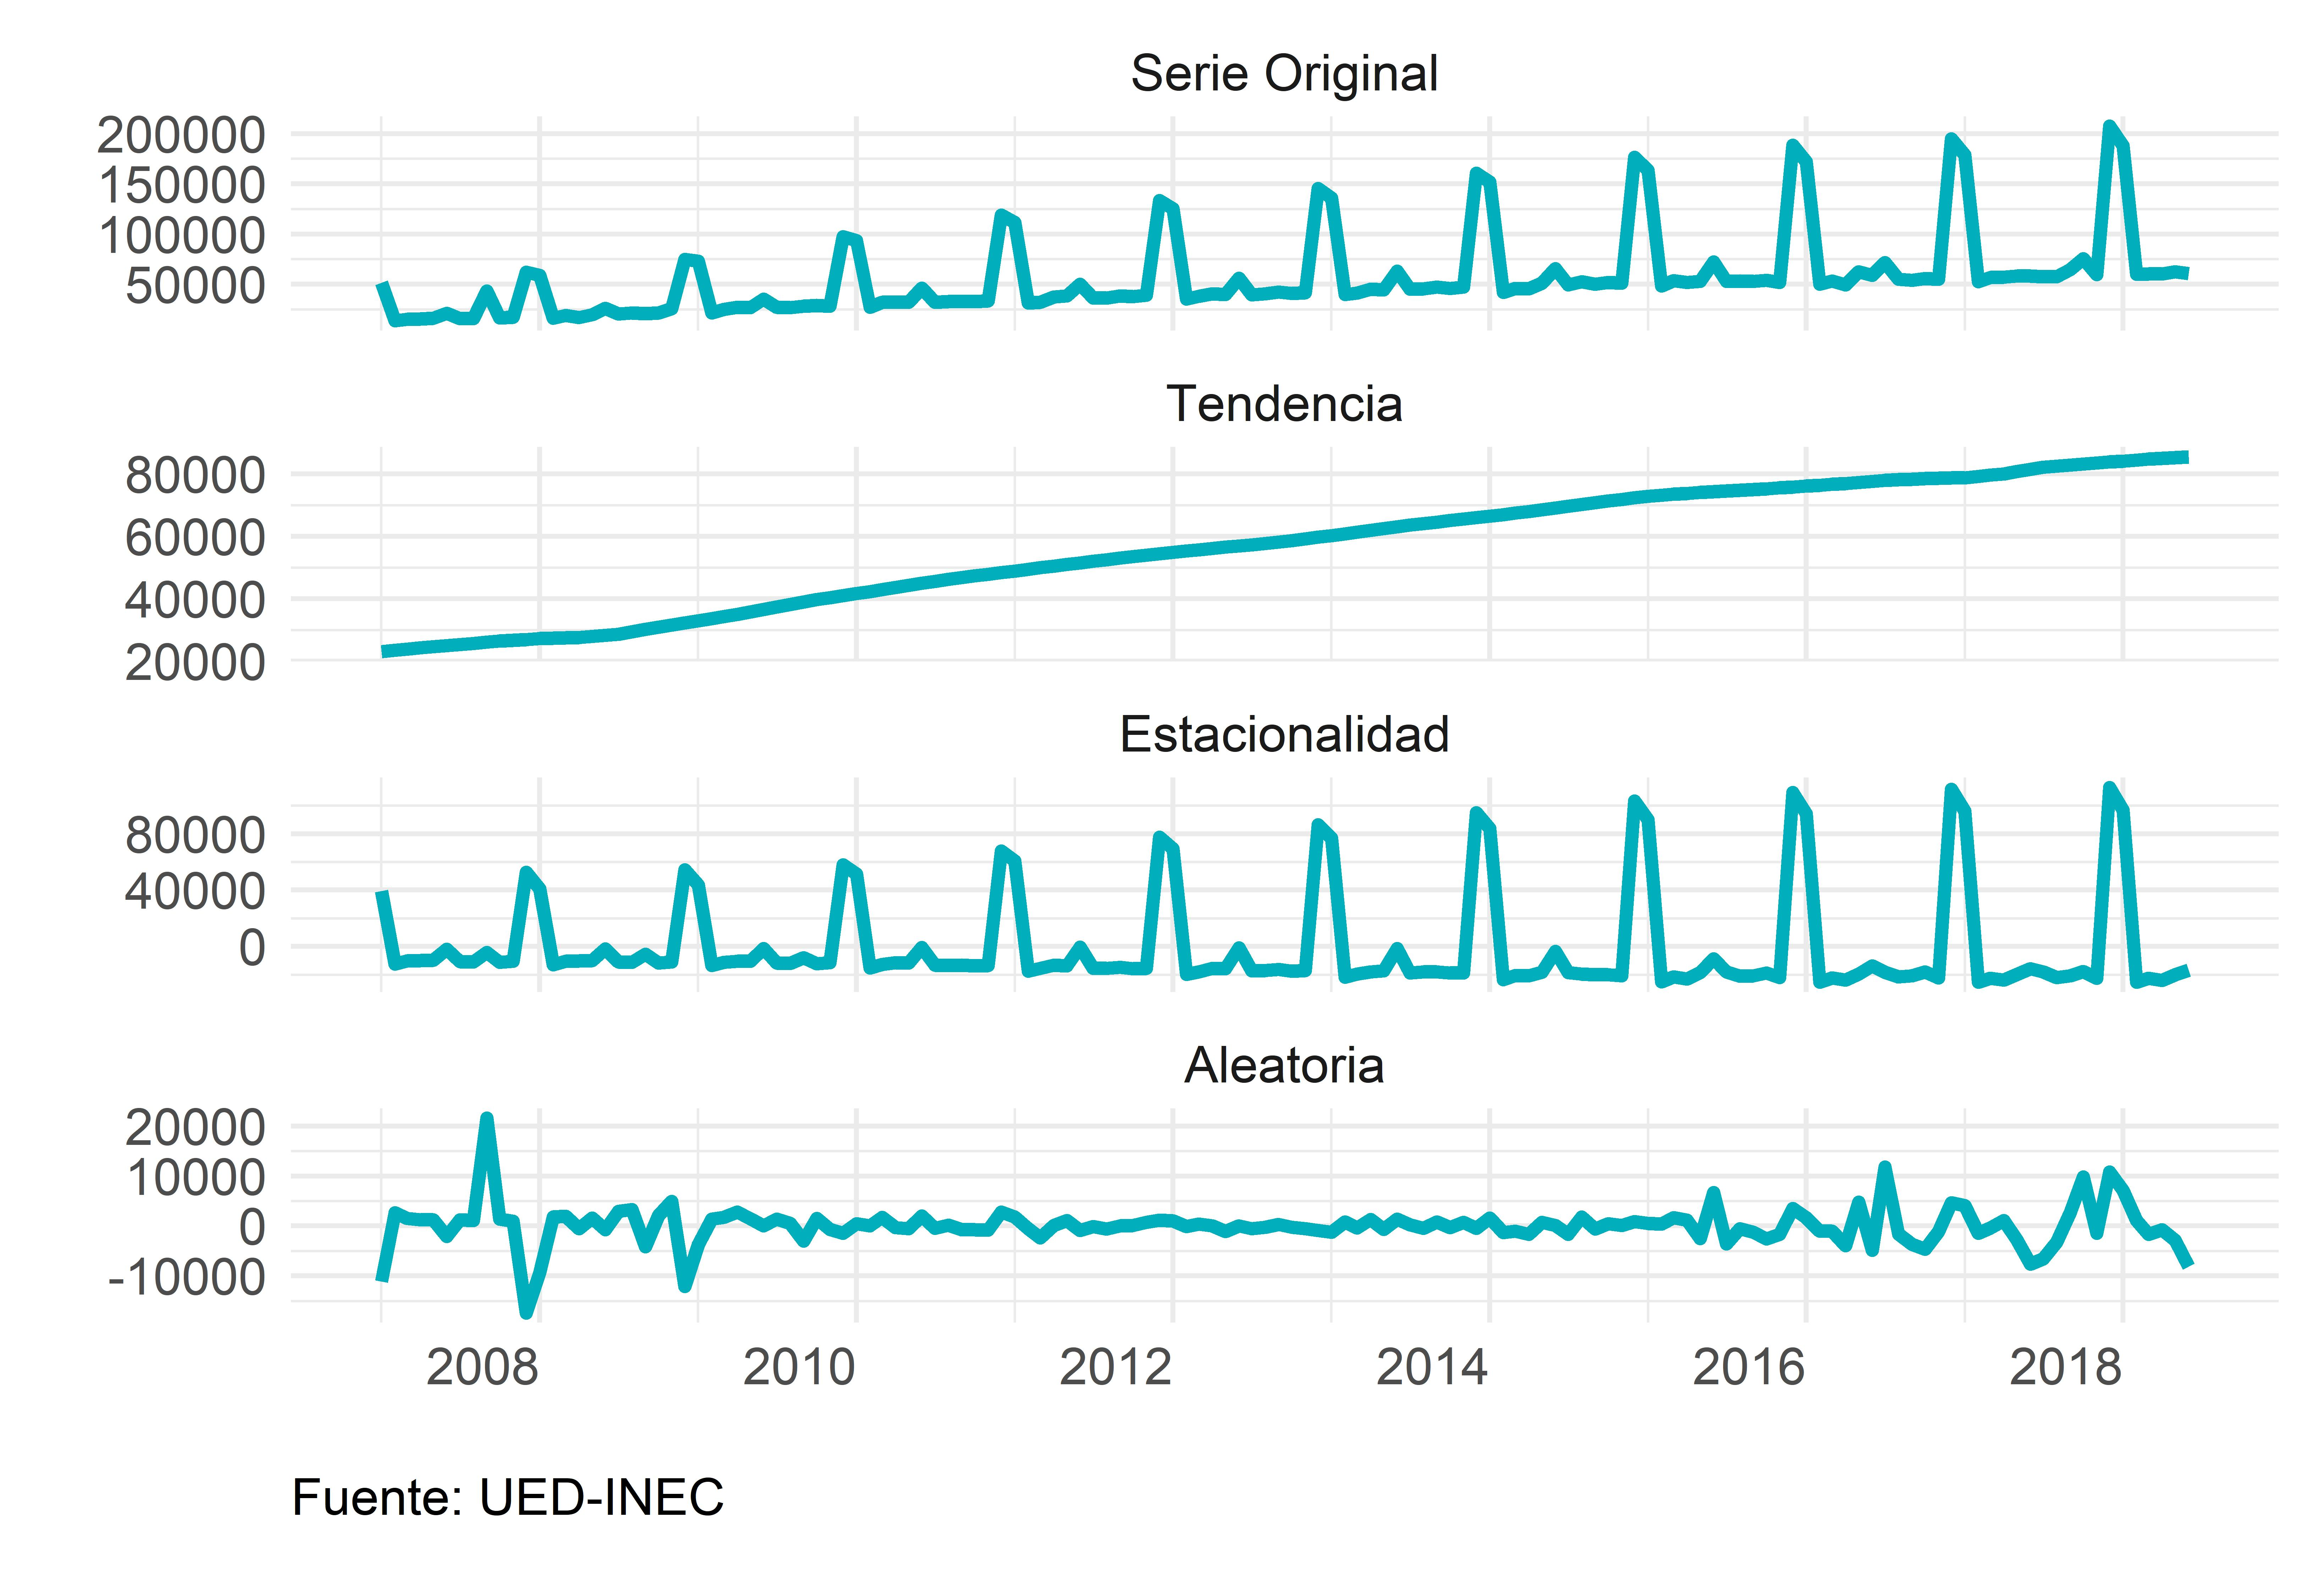
\includegraphics[width=1\linewidth,height=1\textheight]{Tesis_files/figure-latex/incentivosplotdescomposicion-1} \caption{Descomposición de la serie de Incentivos salariales en el periodo 2007 - 2018}\label{fig:incentivosplotdescomposicion}
\end{figure}

\subsubsection{Intereses y comisiones del sector público}

Finalmente, se utiliza para este análisis la serie cronológica de los
intereses y comisiones del sector público, que comprenden el pago de los
intereses de la deuda del gobierno, esto es, las erogaciones de
intereses y comisiones destinadas por las instituciones públicas para
cubrir el pago a favor de terceras personas, físicas o jurídicas, del
sector privado o del sector público, residentes en el territorio
nacional o en el exterior, por la utilización en un determinado plazo de
recursos financieros provenientes de los conceptos de emisión y
colocación de títulos valores, contratación de préstamos directos,
créditos de proveedores, depósitos a plazo y a la vista, intereses por
deudas de avales asumidos, entre otros pasivos de la entidad tranzados
en el país o en el exterior. Incluye el pago por concepto de otras
obligaciones contraídas entre las partes, que no provienen de las
actividades normales de financiamiento. Además, los intereses y
comisiones por las operaciones normales de los bancos comerciales del
sector público, así como las diferencias por tipo de cambio por
operaciones financieras; y también el pago de intereses moratorios
correspondientes a la deuda pública.

Para iniciar el análisis exploratorio de esta serie, la Figura
\ref{fig:interesesplotgeneral} muestra que hay un ligero cambio de
concavidad a partir de Julio 2010, esto sugiere que a partir de este
momento los intereses y comisiones inician una tendencia al alza, la
cual se sostiene hasta Junio del 2018. Por su parte, la Figura
\ref{fig:interesesplotperiodos} muestra cómo hay un crecimiento
sostenido de los intereses y comisiones del sector público al final de
cada trimestre durante todo el periodo, mientras que se mantiene casi
constante durante los primeros dos meses de cada trimestre. La caída más
pronunciada se dio en abril del 2015 mientras que la tasa de crecimiento
más rápida parece darse al final del primer trimestre. Además, en la
Figura \ref{fig:interesesplotdescomposicion} se muestra la
descomposición de la serie en sus distintos componentes. Puede
observarse, además de un crecimiento a lo largo del tiempo posterior a
una disminución, los picos y las caídas en la parte estacional, esto en
cuanto a los cierres trimestrales previamente mencionados. El componente
aleatorio muestra indicios de que la variabilidad de la serie no es
homogénea, sino que cambia conforme pasa el tiempo, pues durante un
tiempo se mantuvo relativamente estable pero luego presenta algunos
cambios.

\begin{figure}[H]
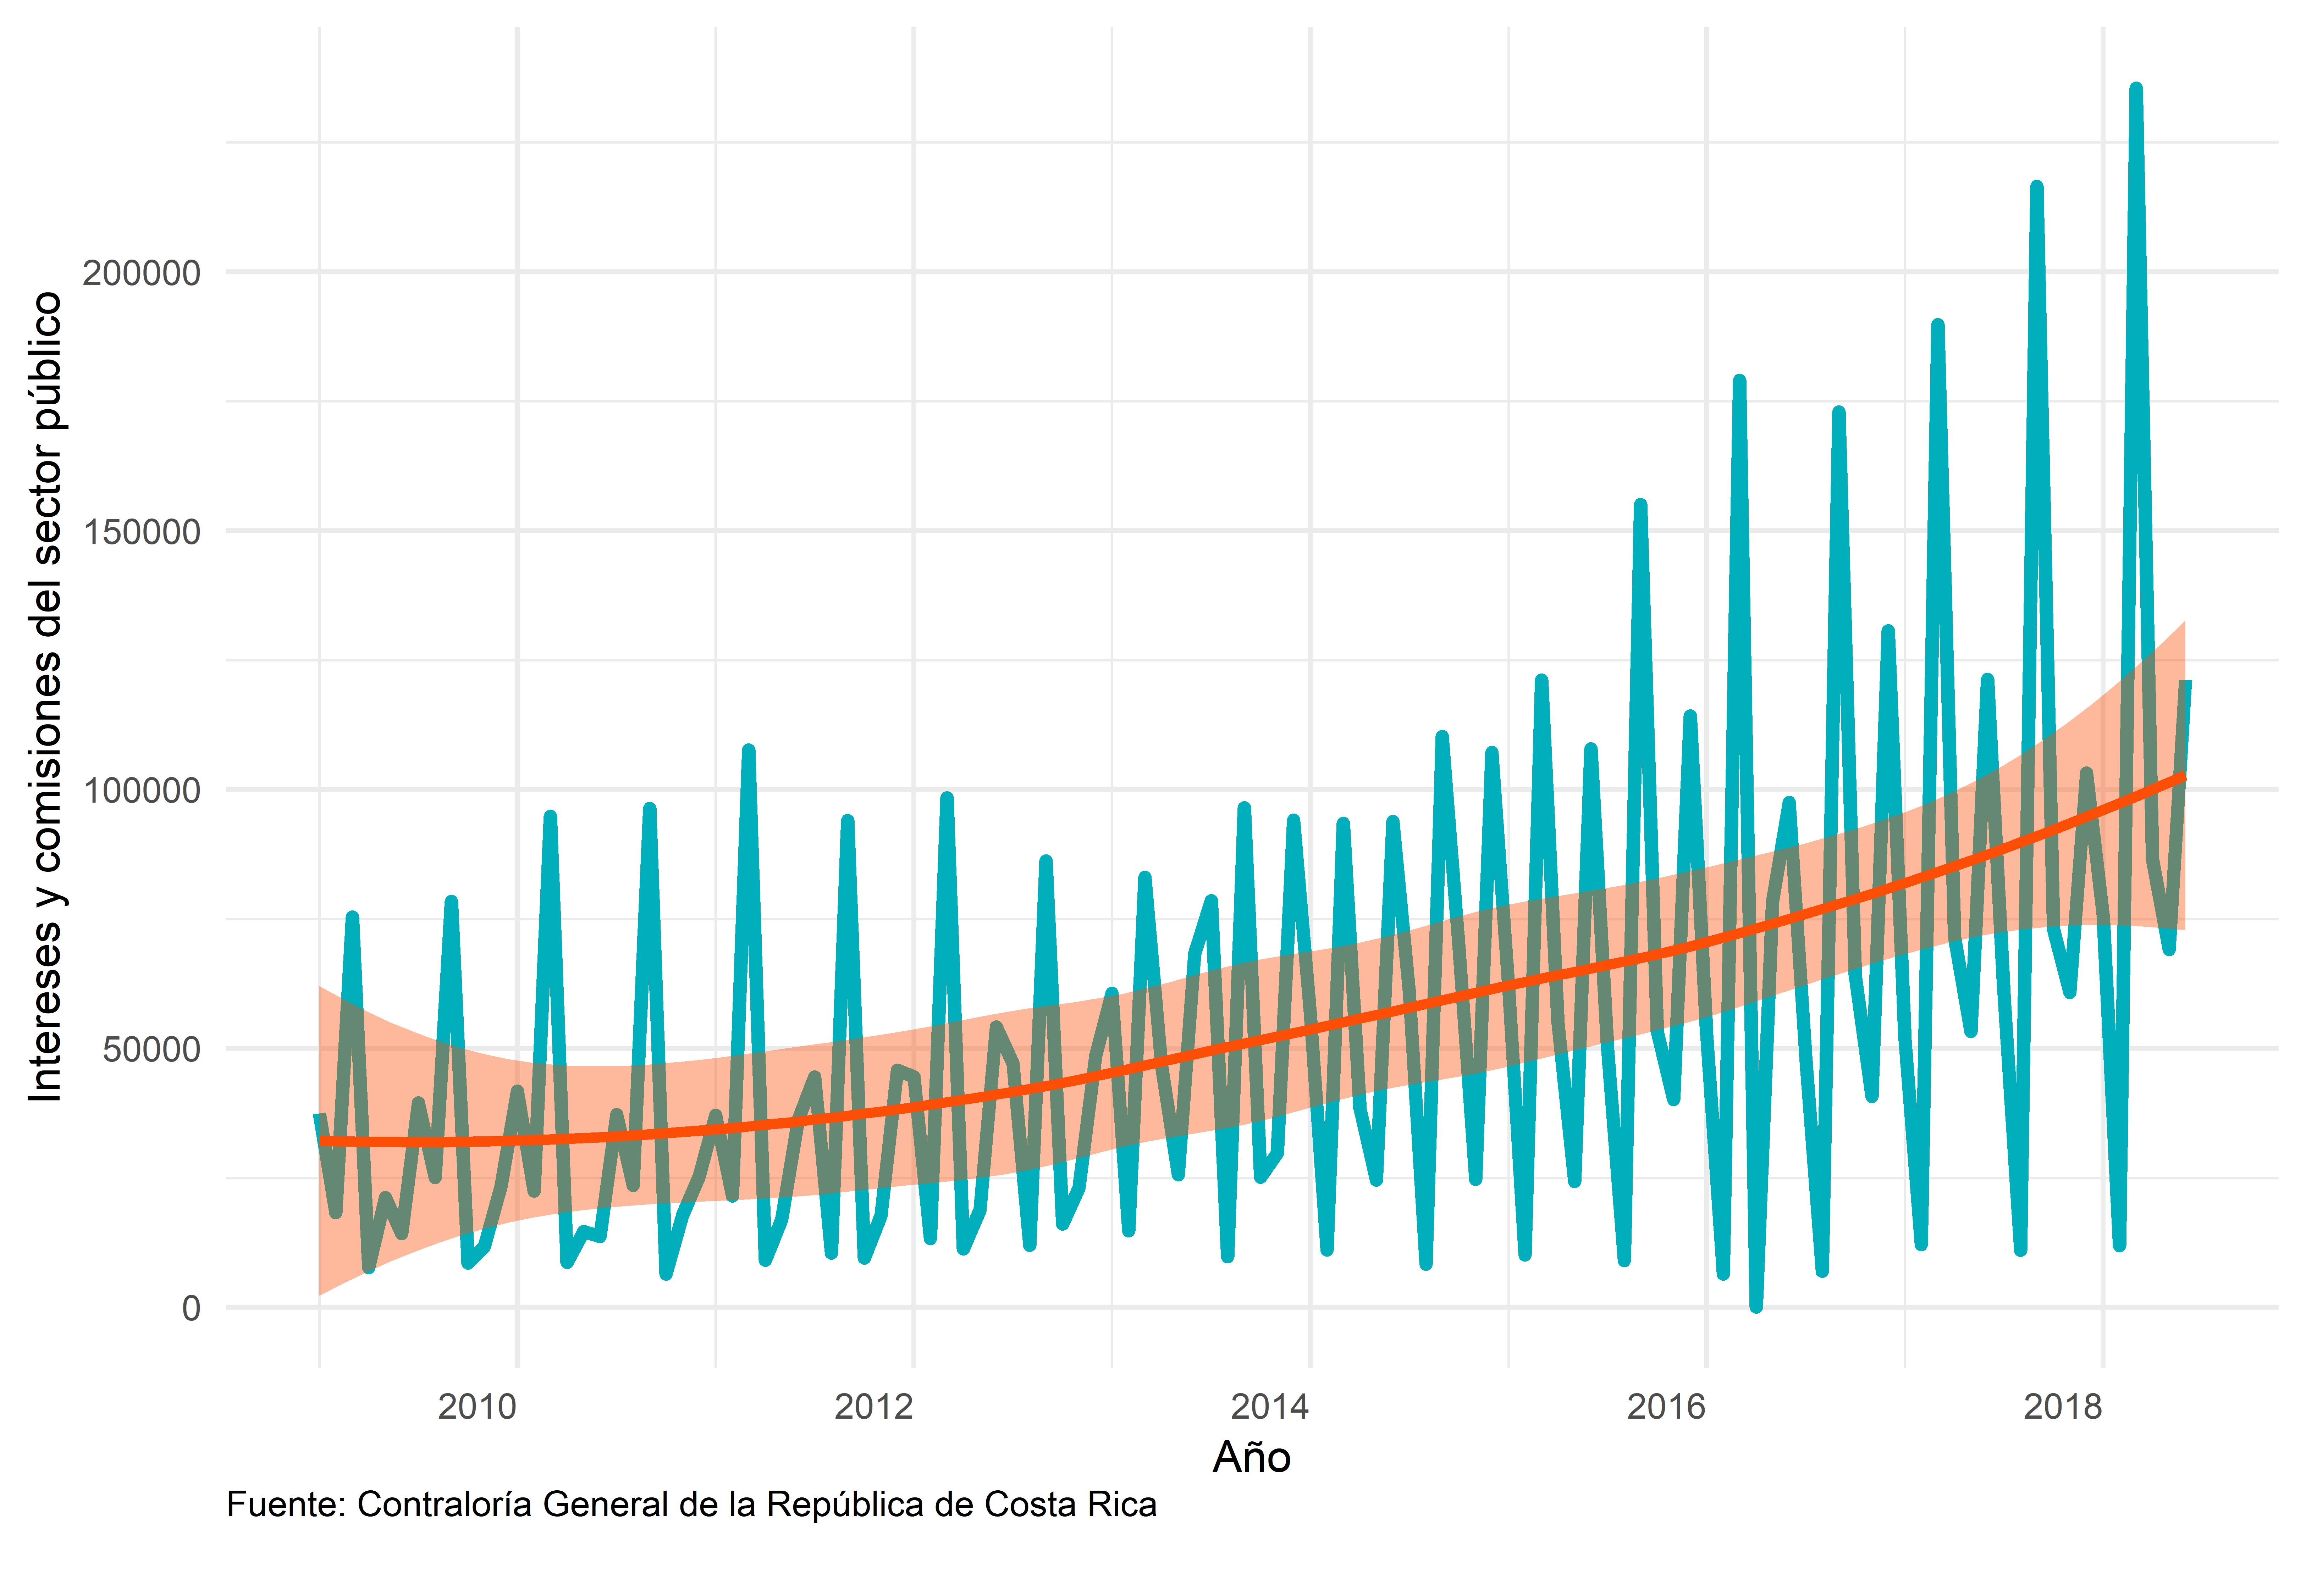
\includegraphics[width=1\linewidth,height=1\textheight]{Tesis_files/figure-latex/interesesplotgeneral-1} \caption{Intereses y comisiones del sector público en el periodo 2007-2018}\label{fig:interesesplotgeneral}
\end{figure}

\begin{figure}[H]
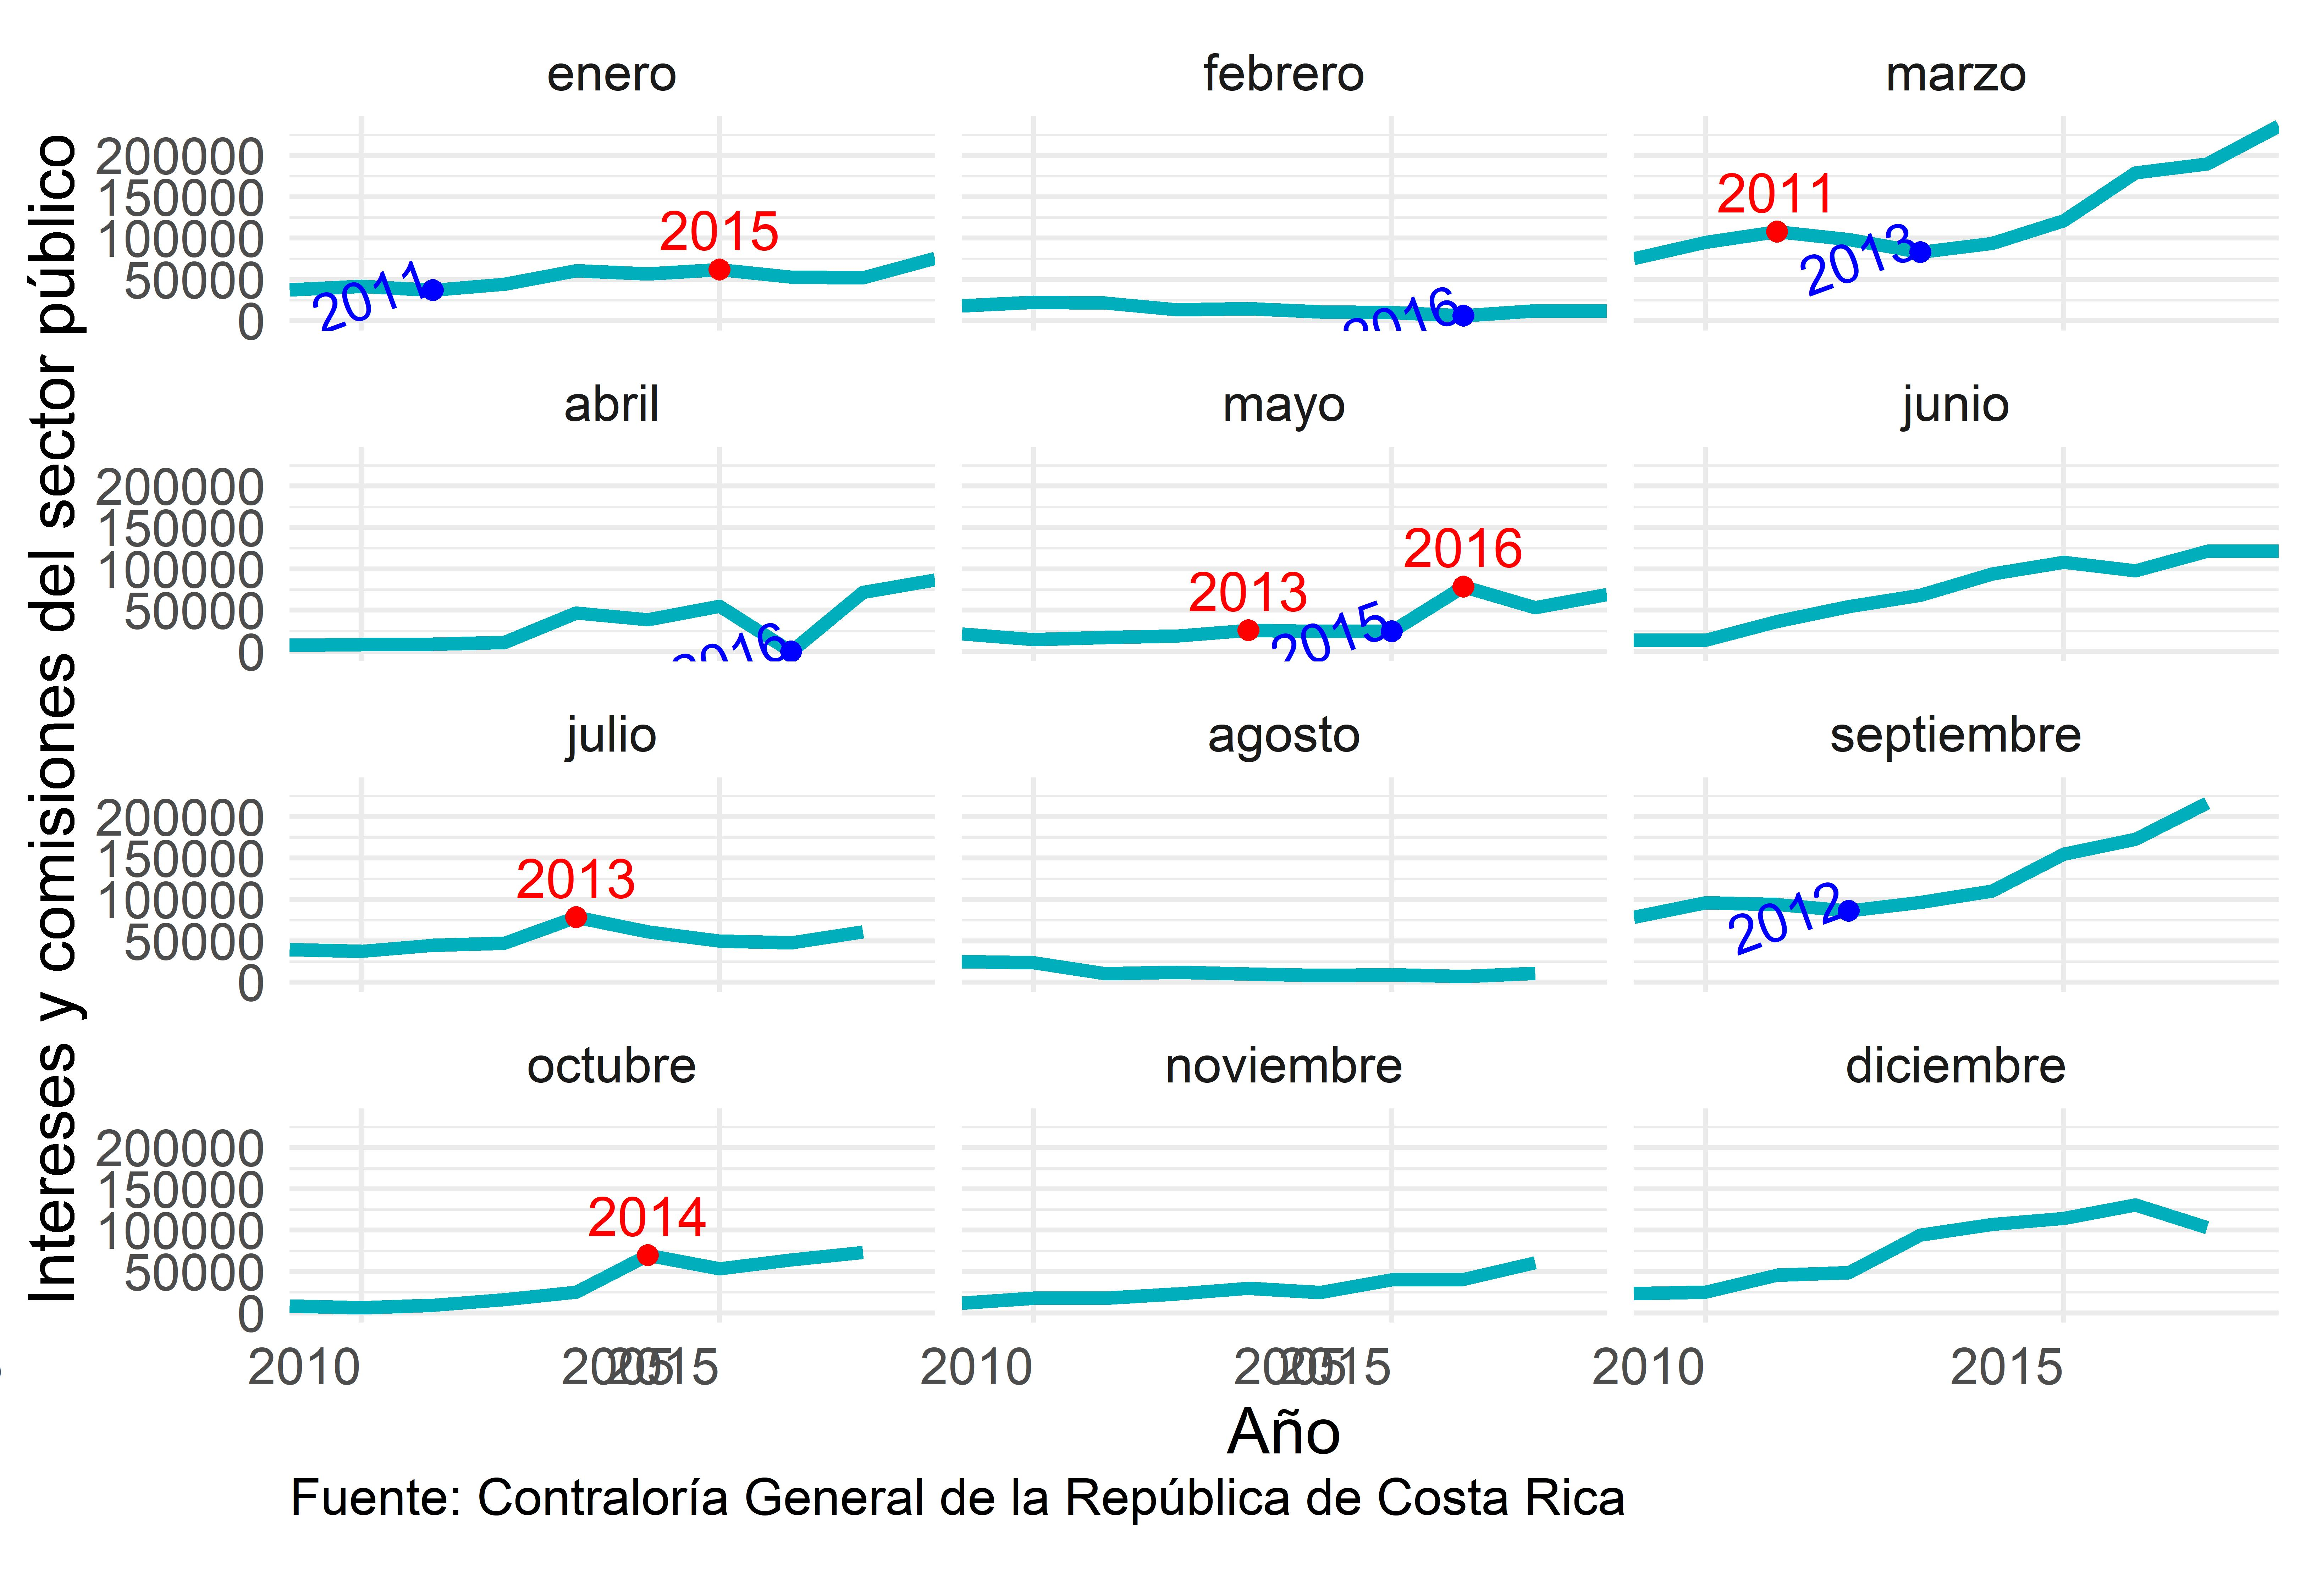
\includegraphics[width=1\linewidth,height=1\textheight]{Tesis_files/figure-latex/interesesplotperiodos-1} \caption{Intereses y comisiones del sector público en el periodo 2007-2018 según mes}\label{fig:interesesplotperiodos}
\end{figure}

En la Figura \ref{fig:interesesplotdescomposicion} se muestra la
descomposición de la serie en sus distintos componentes. Pueden
observarse, además de un crecimiento a lo largo del tiempo posterior a
una disminución, los picos y las caídas en la parte estacional. El
componente aleatorio muestra indicios de que la variabilidad de la serie
no es homogénea, sino que cambia conforme pasa el tiempo, pues durante
un tiempo se mantuvo relativamente estable pero luego presenta algunos
cambios.

\begin{figure}[H]
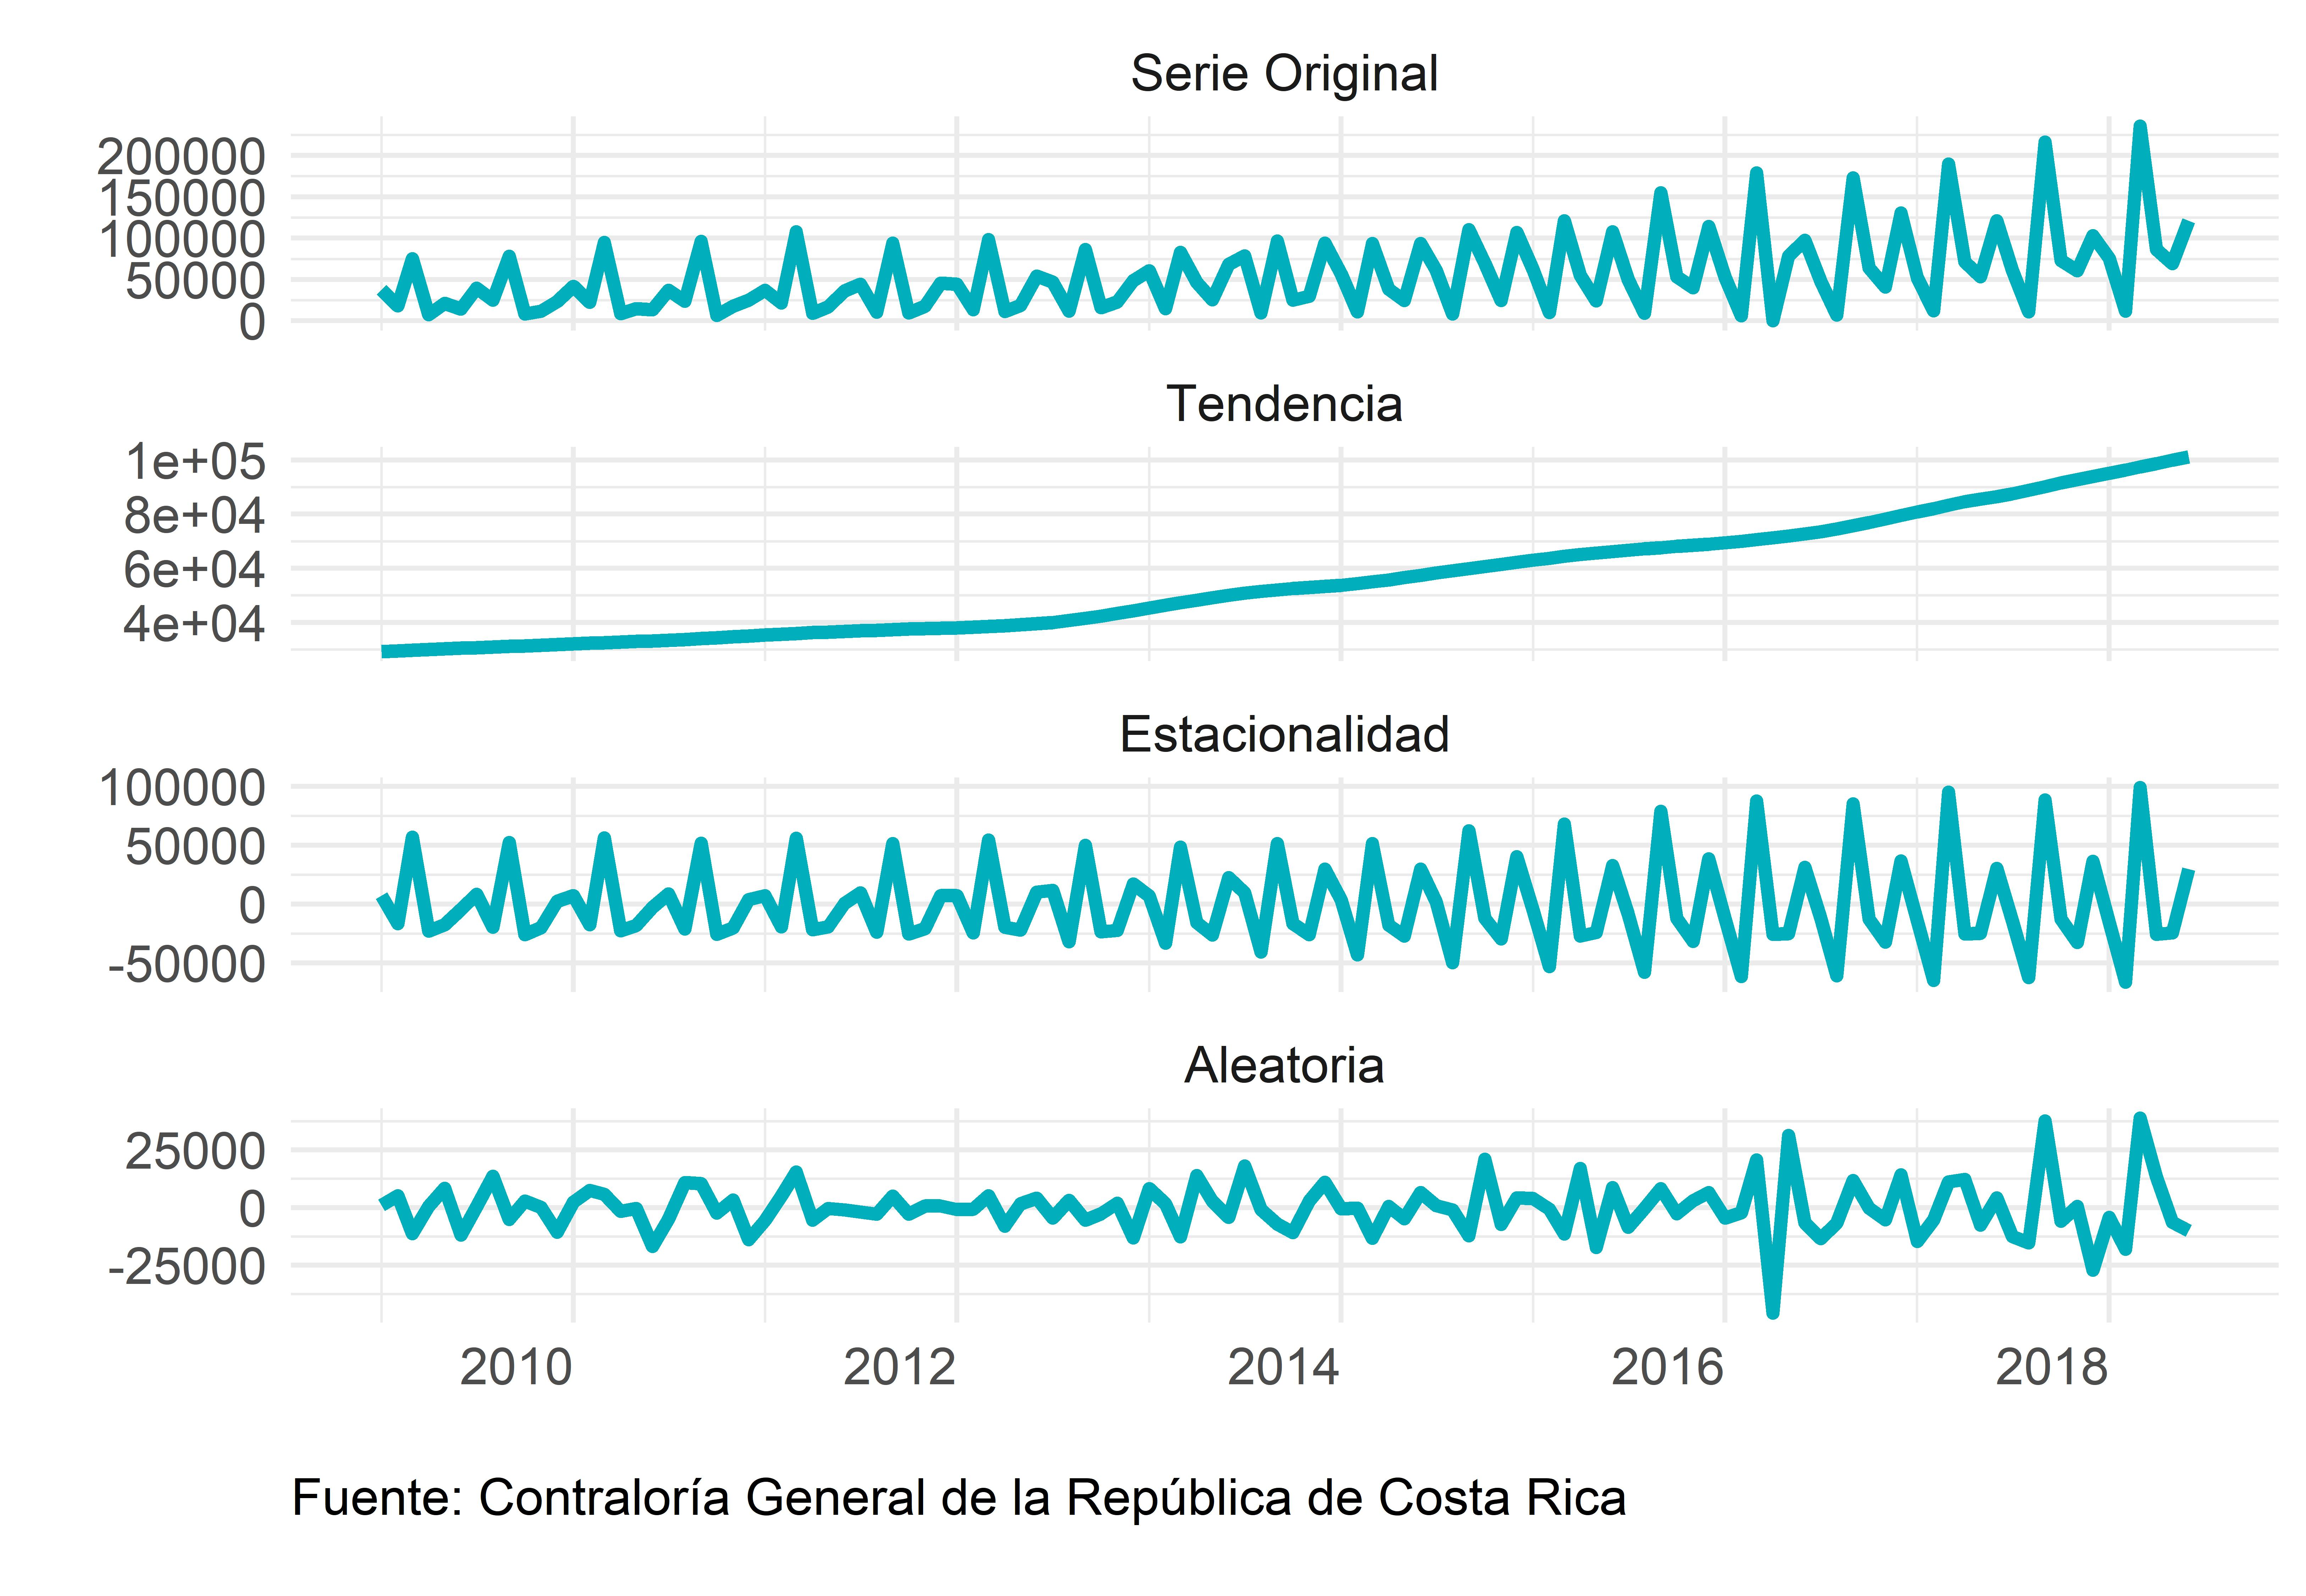
\includegraphics[width=1\linewidth,height=1\textheight]{Tesis_files/figure-latex/interesesplotdescomposicion-1} \caption{Descomposición de la serie de Incentivos salariales en el periodo 2007 - 2018}\label{fig:interesesplotdescomposicion}
\end{figure}

\subsubsection{Herramientas analíticas y procedimiento de simulación}

Como se ha mencionado en este documento, el lenguaje de programación R
ha sido utilizado para los análisis. Específicamente, los paquetes
utilizados para la obtención de estos resultados, aparte de los ya
mencionados, son \texttt{knitr} (\protect\hyperlink{ref-knitr}{Xie,
2014}), \texttt{kableExtra} (\protect\hyperlink{ref-kableExtra}{Zhu,
2021}), \texttt{readxl} (\protect\hyperlink{ref-readxl}{Wickham \&
Bryan, 2019}), \texttt{gridExtra}
(\protect\hyperlink{ref-gridExtra}{Auguie, 2017}), \texttt{ggpubr}
(\protect\hyperlink{ref-ggpubr}{Kassambara, 2020}), \texttt{ggplot2}
(\protect\hyperlink{ref-ggplot2}{Wickham, 2016}), \texttt{lubridate}
(\protect\hyperlink{ref-lubridate}{Grolemund \& Wickham, 2011}),
\texttt{ggseas} (\protect\hyperlink{ref-ggseas}{Ellis, 2018}),
\texttt{ggpmisc} (\protect\hyperlink{ref-ggpmisc}{Aphalo, 2021}) y
\texttt{forecast} (\protect\hyperlink{ref-forecast}{Hyndman \&
Khandakar, 2008}).

La metodología propuesta será puesta a prueba en una primera etapa con
series cronológicas simuladas a partir de distintos modelos. Los
resultados obtenidos al utilizar la sobreparametrización serán
contrastados con otros dos métodos: La función \texttt{auto.arima()} de
R y un modelo ARIMA estándar, que se trata de un \(ARIMA(1,1,1)\) en el
caso de series no estacionales, y un \(ARIMA(1,1,1)(1,1,1)_{12}\) sobre
los datos simulados de series mensuales. De forma similar, se comparan
los resultados obtenidos mediante la sobreparametrización con los
obtenidos utilizando la función \texttt{auto.arima()} de R, aplicado a
las distintas series cronológicas.

Como parte de esta investigación, es necesario validar la estimación de
modelos ARIMA mediante sobreparametrización no solo con datos reales,
sino también mediante datos simulados. Para ello es necesario generar
series cronológicas que son gobernadas por un proceso determinado y
previamente conocido para poder compararlo con los modelos identificados
tanto con la sobreparametrización, como con la función
\texttt{auto.arima()} y el correspondiente modelo \(ARIMA\) estándar.

Con este fin, se programó una función que sigue los siguientes pasos
(también mostrados en la figura \ref{fig:diagrama_flujo_simulacion}:

\textbf{1.} Se generan valores aleatorios de alguna distribución de
probabilidad. Para esta investigación se escogen 100 valores de una
distribución Normal con media 10 y varianza 1. Estos valores se resumen
en la Figura \ref{fig:datos_simulados}; donde las región azul oscuro
representa la densidad de datos entre los percentiles 25 y 75, las
líneas punteadas de color naranja marcan la cantidad de desviaciones
estándar que los datos se alejan del promedio, y las líneas punteadas de
color azul marcan los puntos de corte mínimo, percentiles 25, 50 y 75, y
el máximo.

\textbf{2.} Se seleccionan mediante un muestreo simple al azar la
cantidad de coeficientes a utilizar en los términos del modelo
\(ARIMA(p,d,q)(P,D,Q)_S\) que gobierna la serie. Para esta investigación
fueron seleccionados los siguientes procesos:
\(ARIMA(1,0,0), ARIMA(1,0,1),\) \(ARIMA(2,0,3), ARIMA(4,0,2),\)
\(ARIMA(0,0,1)(0,1,1)_{12}\) y \(ARIMA(2,1,4)(3,0,3)_{12}\).

\textbf{3.} Para cada uno de los procesos seleccionados, se generan
valores aleatorios de una distribución uniforme con un valor mínimo de 0
y un valor máximo de 0.99. La cantidad de valores simulados depende de
la cantidad de parámetros escogidos en \(p, q, P, Q\). Estos valores
aleatorios son transformados de manera tal que los polinomios de la
parte autorregresiva y de medias móviles no comparta raíces unitarias,
este es un proceso iterativo que se completa hasta que los coeficientes
obtenidos tanto para la parte autorregresiva como para la parte de
medias móviles generen un proceso invertible y estacionario.

\textbf{4.} Con los valores simulados, la cantidad de parámetros y sus
respectivos valores definidos en los puntos anteriores, se ajusta cada
uno de los modelos \(ARIMA\) descritos en el inciso \textbf{2.}.

\textbf{5.} Con cada modelo ajustado, se utiliza la función
\texttt{simulate.Arima()} para generar 200 observaciones basadas en
dichos modelos.

\begin{figure}[H]
\includegraphics[width=1\linewidth,height=1\textheight]{Tesis_files/figure-latex/diagrama_flujo_simulacion-1} \caption{Diagrama de flijo del proceso de simulación de las series cronológicas.}\label{fig:diagrama_flujo_simulacion}
\end{figure}

Tras aplicar los pasos anteriores y obtener las correspondientes series
cronológicas simuladas, el comportamiento y proceso gobernante de cada
una se muestra en la Figura \ref{fig:series_simuladas}.

\begin{figure}[H]
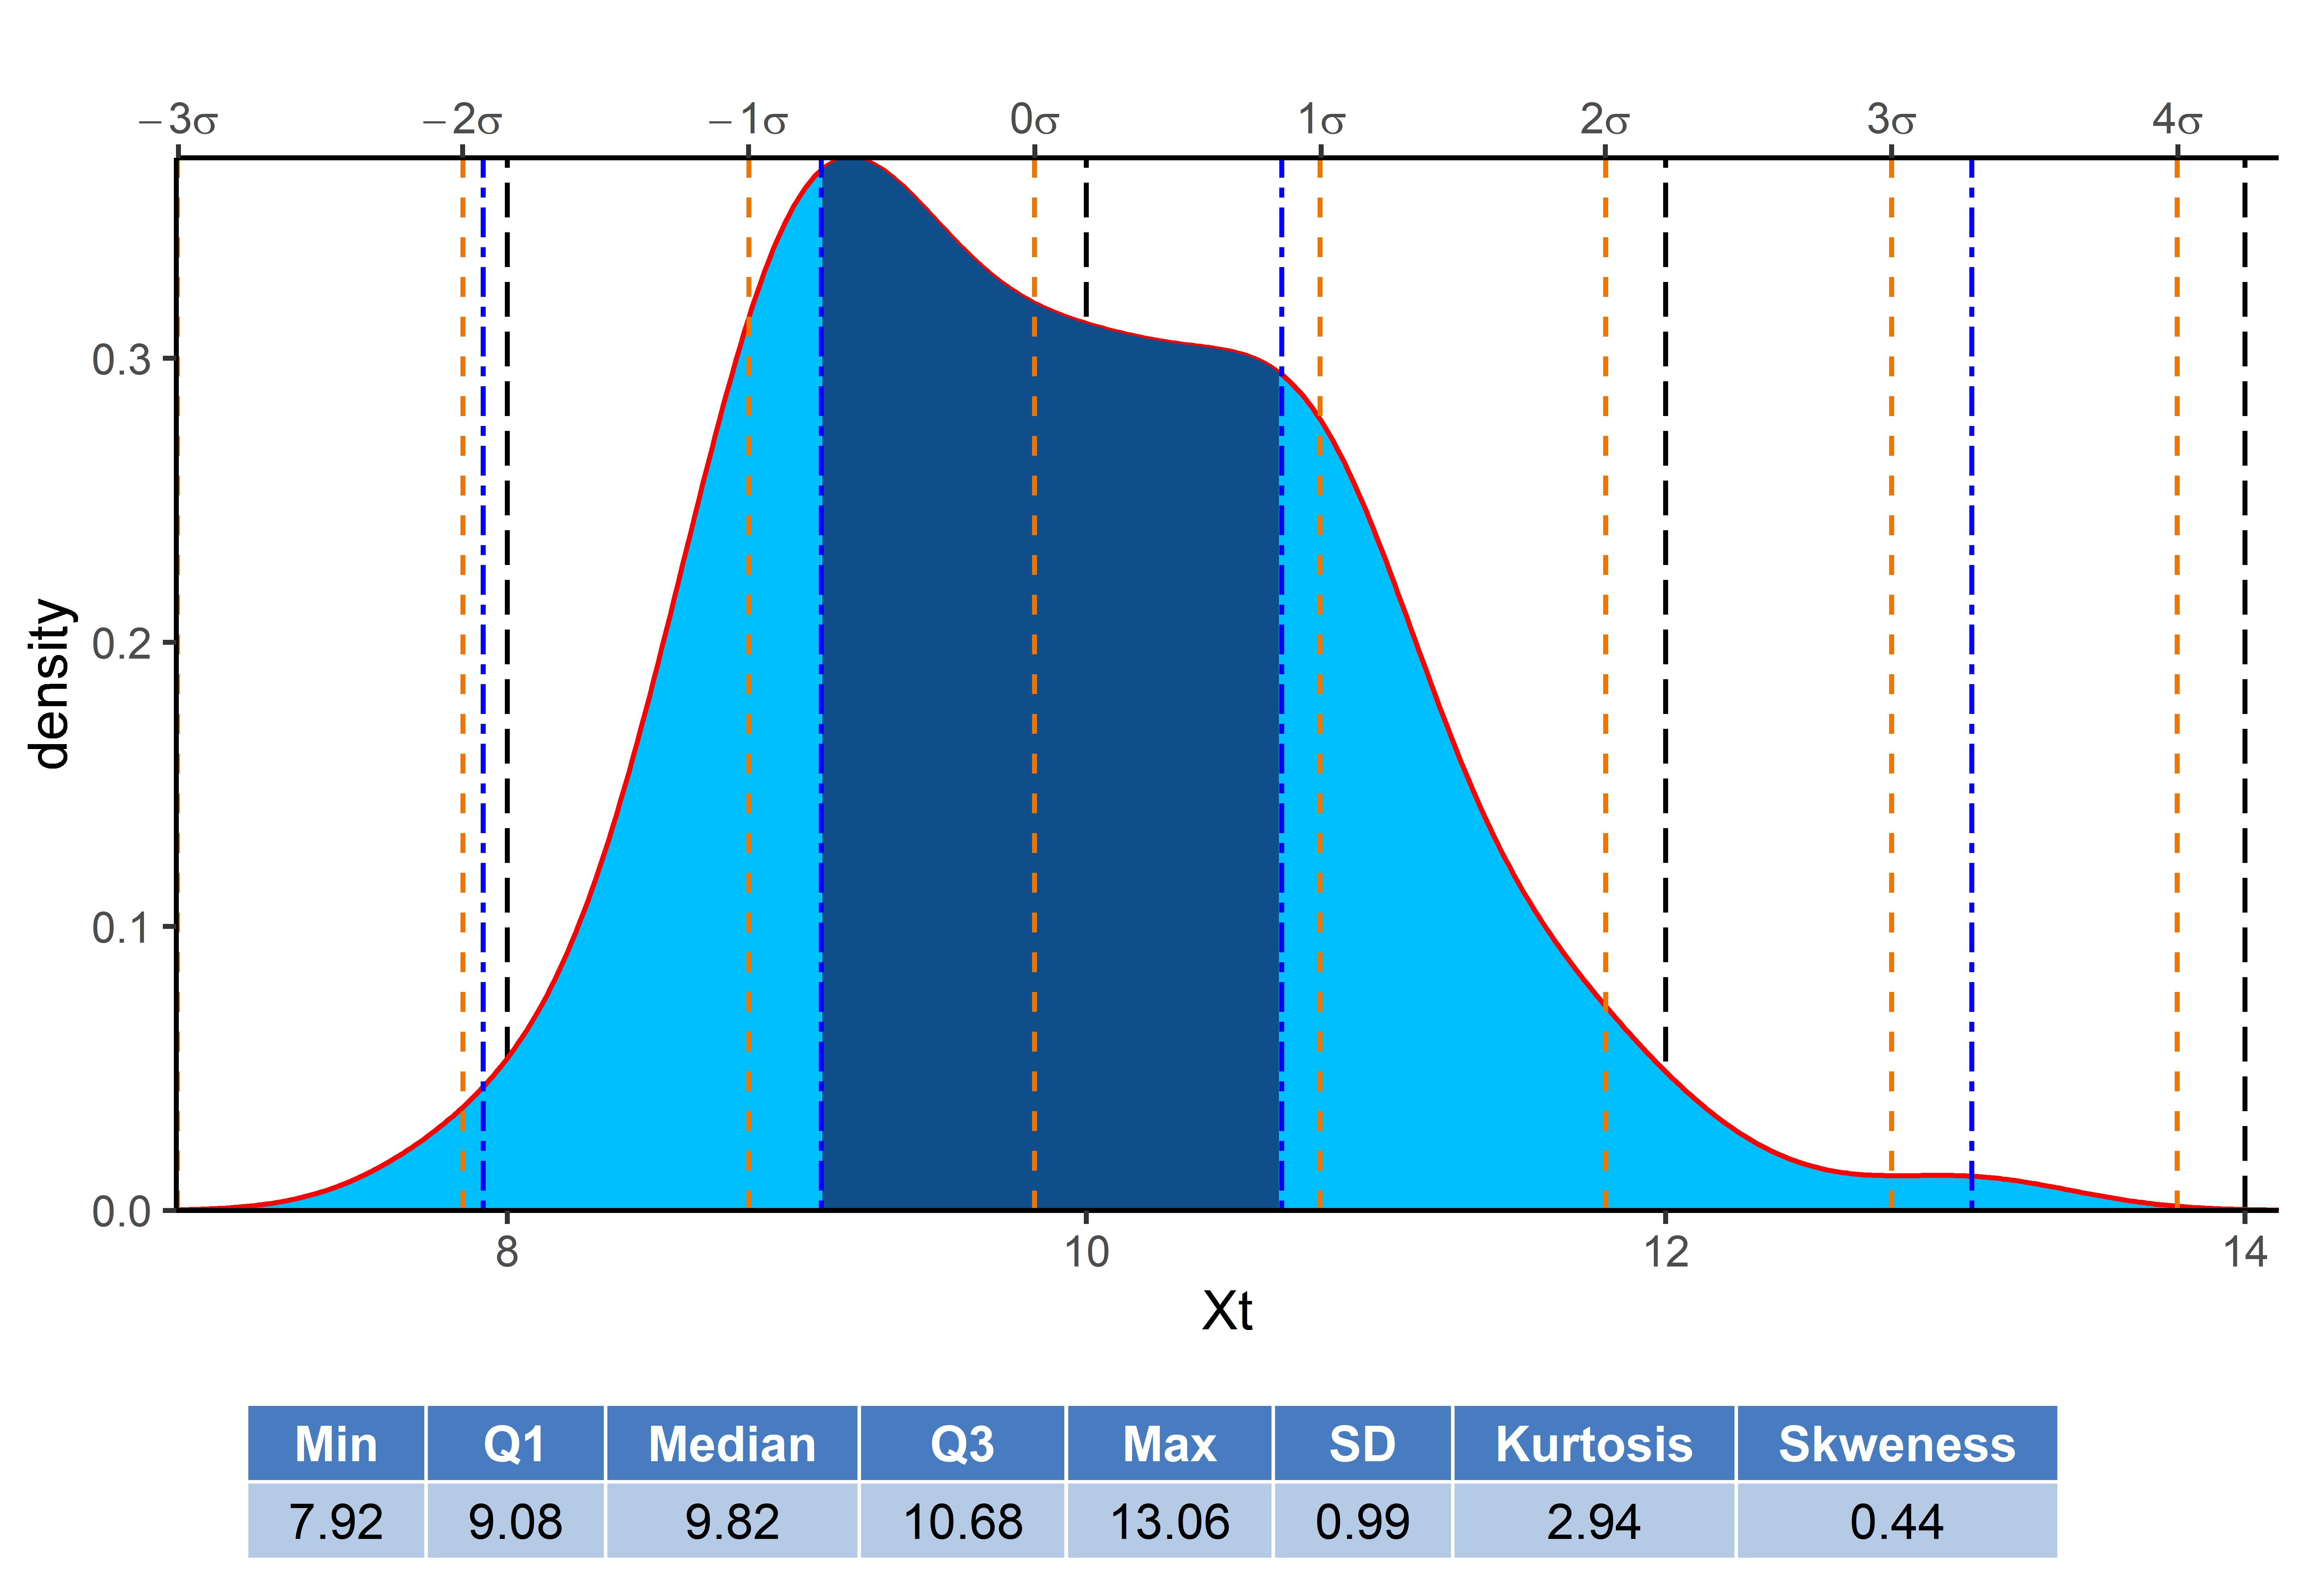
\includegraphics[width=1\linewidth,height=1\textheight]{Tesis_files/figure-latex/datos_simulados-1} \caption{Valores de referencia para la simulación de series cronológicas}\label{fig:datos_simulados}
\end{figure}

\begin{figure}[H]
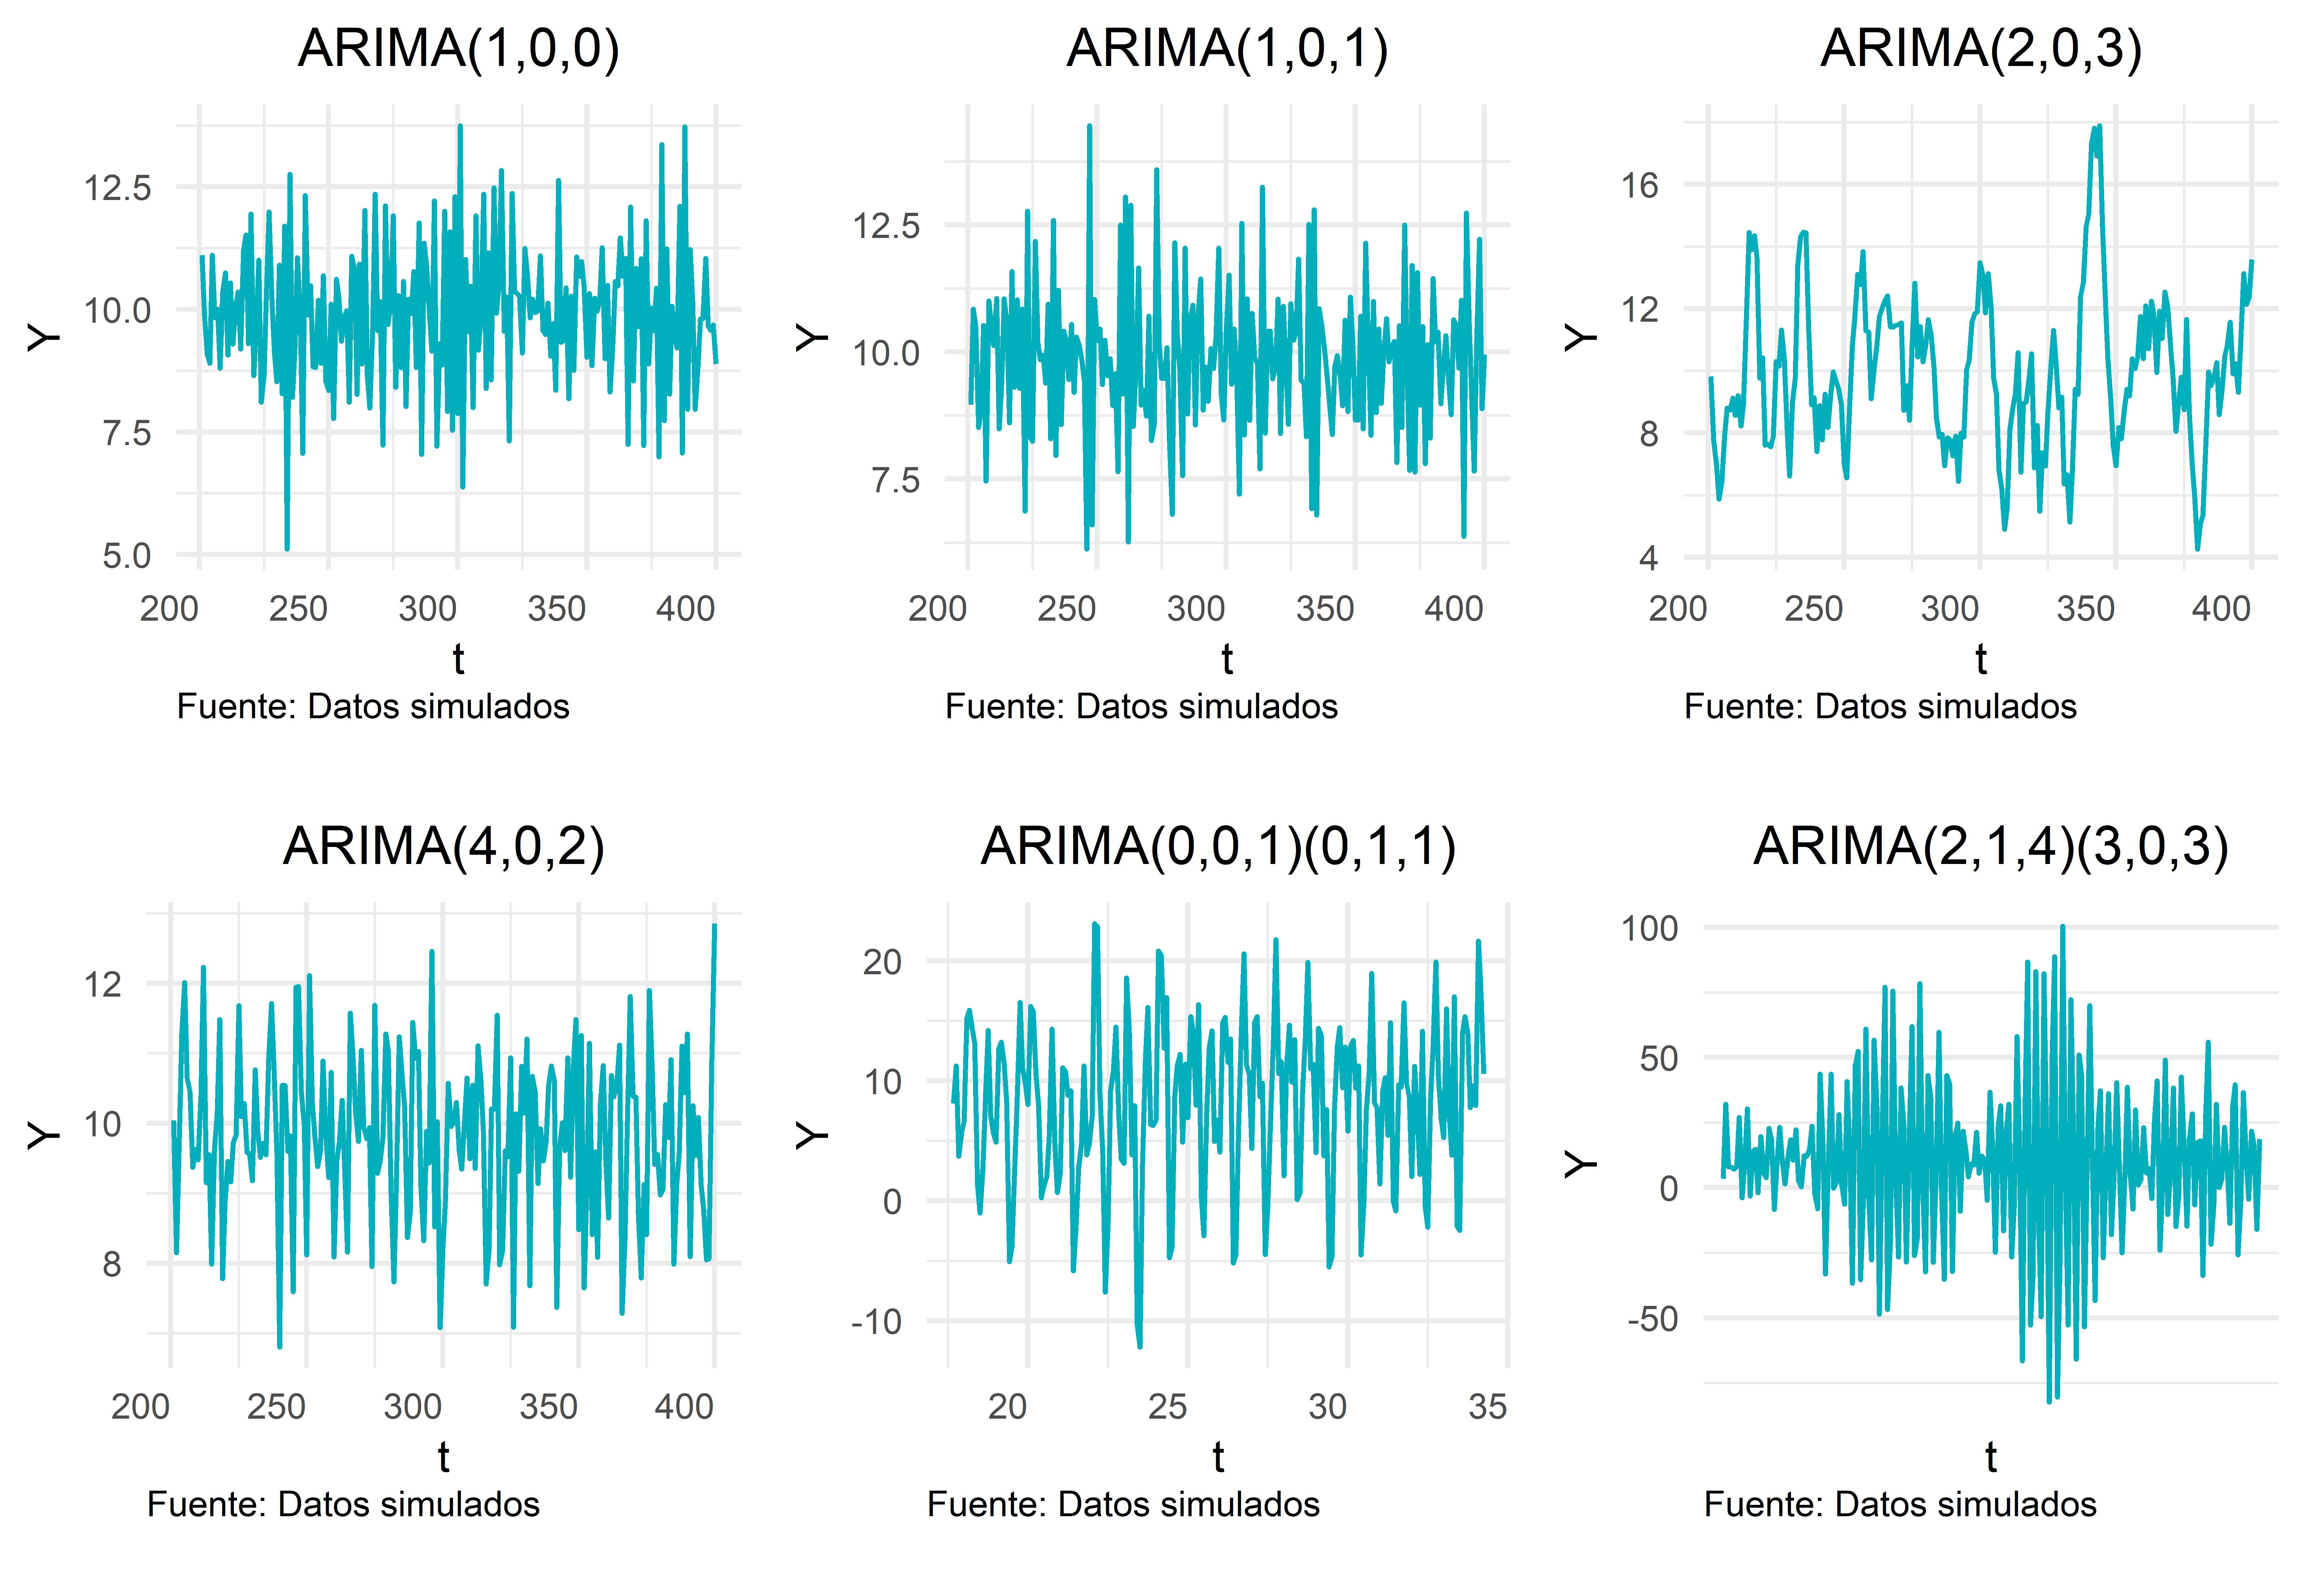
\includegraphics[width=1\linewidth,height=1\textheight]{Tesis_files/figure-latex/series_simuladas-1} \caption{Series cronológicas simuladas}\label{fig:series_simuladas}
\end{figure}

\subsection{Métodos}

En este apartado se describe el procedimiento a seguir con cada una de
las series cronológicas mencionadas previamente, tanto las series
simuladas como las reales. Para comprobar el poder predictivo del método
propuesto se realiza inicialmente un análisis exploratorio para
verificar si las series temporales sujetas a análisis son o no
estacionarias, y en caso de no serlo, si requieren algún proceso de
diferenciación. Se describe además el proceso de partición de los datos
tanto para ajustar los modelos como para validar los pronósticos. Para
cada serie de tiempo, se estima el mejor modelo utilizando la función
\texttt{auto.arima()}, la sobreparametrización y un modelo ARIMA
estándar, que puede ser un \(ARIMA(1,1,1)\) para las series no
estacionales, o un \(ARIMA(1,1,1)(1,1,1)_S\) en el caso de las series
cronológicas estacionales. Una vez obtenidos estos modelos, se analizan
los residuales obtenidos. En última instancia, se obtienen los
pronósticos y sus medidas de bondad de ajuste y de rendimiento.

\subsubsection{Análisis exploratorio}

Como fue mencionado en el Marco Teórico, debe corroborarse que la serie
cronológica a trabajar posea un comportamiento estacionario y, de no
serlo, someterla a transformaciones para asegurar esta condición,
estando entre los más comunes la diferenciación o la aplicación del
logaritmo natural. Posteriormente, se realiza una identificación del
posible proceso que gobierna la serie cronológica al graficar las
funciones de autocorrelación y autocorrelación parcial, las cuales
también sirven para verificar si la serie (transformada o no) es
estacionaria.

\subsubsection{Partición de los datos}

A partir de la serie cronológica que se someterá a análisis, se realiza
una partición de los datos para tener dos conjuntos distintos:
entrenamiento y validación. El primero servirá precisamente para
entrenar y estimar los distintos modelos; mientras que el segundo
servirá para validar los pronósticos obtenidos. De manera
predeterminada, se utilizará una partición del 80\% de los datos para el
conjunto de entrenamiento y un 20\% para los datos de validación, sin
embargo, esto puede cambiar de acuerdo al interés propio del(la)
investigador(a).

\subsubsection{Identificación y estimación del mejor modelo según la función auto.arima()}

Con el correspondiente conjunto de datos de entrenamiento, se utiliza la
función \texttt{auto.arima()} para encontrar el mejor modelo ARIMA
sugerido con este método, que como fue mencionado en la introducción de
esta tesis, usa como criterio la minimización del AICc.

\subsubsection{Identificación y estimación del mejor modelo con sobreparametrización}

A partir del mismo conjunto de datos de entrenamiento de la
correspondiente serie cronológica, se utiliza la sobreparametrización
para encontrar el mejor modelo a partir de distintas permutaciones de la
cantidad de coeficientes de los términos \(p,d,q, P,D,Q\), según sea el
caso.

La estimación de los modelos y posterior selección de los mismos vía
sobreparametrización es un proceso que requiere de distintas etapas. El
procedimiento completo fue programado utilizando el lenguaje R, el cuál
fue construido haciendo uso de los paquetes de R \texttt{tidyr}
(\protect\hyperlink{ref-tidyr}{Wickham \& Henry, 2019}),
\texttt{dplyr}(\protect\hyperlink{ref-dplyr}{Wickham et al., 2019}) y
\texttt{parallel}(\protect\hyperlink{ref-parallel}{R Core Team, 2019}),
los procesos internos de esta función son descritos a continuación:

\textbf{1.} Una vez que se define la partición que tendrá la serie
cronológica, se prosigue con la selección de los escenarios para estimar
los modelos de ARIMA. Es en esta instancia en donde se decide el valor
máximo de los parámetros \(p,d,q,P,D,Q\) del modelo
\(ARIMA(p,d,q)(P,D,Q)_s\) que serán sujetos al análisis.

\textbf{2.} Para el caso de series cronológicas no estacionales, los
valores \(P,D\) y \(Q\) son iguales a cero (porque precisamente, no se
estiman coeficientes para la parte estacional). Se estiman para esta
investigación todas las permutaciones de parámetros \(p,d,q\) hasta
tener como máximo un modelo \(ARIMA(6,1,6)\), aunque el orden del modelo
más grande puede permitir un mayor número de diferenciaciones o de
parámetros. Para ello se genera una matriz con cada una de estas
permutaciones, denominada matriz de valores paramétricos, en donde cada
fila representa la especificación del modelo \(ARIMA(p,d,q)\) que se va
a estimar, tal y como se muestra en \ref{eqn:matriz_arima_1}:

\begin{equation}
\label{eqn:matriz_arima_1}
\begin{tikzpicture}[mymatrixenv]
    \matrix[mymatrix] (m)  {
        0 & 0 & 1 & 0 & 0 & 0 \\
        0 & 0 & 2 & 0 & 0 & 0 \\
        0 & 0 & 3 & 0 & 0 & 0 \\
        0 & 0 & 4 & 0 & 0 & 0 \\
        0 & 0 & 5 & 0 & 0 & 0 \\
        0 & 0 & 6 & 0 & 0 & 0 \\
        0 & 1 & 0 & 0 & 0 & 0 \\
        0 & 1 & 1 & 0 & 0 & 0 \\
        0 & 1 & 2 & 0 & 0 & 0 \\
        \vdots & \vdots & \vdots & \vdots & \vdots & \vdots \\
        6 & 1 & 6 & 0 & 0 & 0 \\
    };
    \mymatrixbracetop{1}{3}{$p, d, q$};
    \mymatrixbracetop{4}{6}{$P,D,Q$}
\end{tikzpicture}
\end{equation}

\textbf{3.} De manera análoga, al trabajar con series cronológicas
estacionales, se decide trabajar (para una temporalidad determinada,
como mensual) hasta un modelo máximo de \(ARIMA(4,1,4)(4,1,4)_{12}\).
Así, la matriz de valores paramétricos mostrada en
\ref{eqn:matriz_arima_2} posee, en cada línea, una especificación de
modelo a estimar:

\begin{equation}
\label{eqn:matriz_arima_2}
\begin{tikzpicture}[mymatrixenv]
    \matrix[mymatrix] (m)  {
        0 & 0 & 1 & 0 & 0 & 1 \\
        0 & 0 & 1 & 0 & 0 & 2 \\
        0 & 0 & 1 & 0 & 0 & 3 \\
        0 & 0 & 1 & 0 & 0 & 4 \\
        0 & 0 & 1 & 0 & 1 & 1 \\
        0 & 0 & 1 & 0 & 1 & 2 \\
        0 & 0 & 1 & 0 & 1 & 3 \\
        \vdots & \vdots & \vdots & \vdots & \vdots & \vdots \\
        4 & 1 & 4 & 4 & 1 & 4 \\
    };
    \mymatrixbracetop{1}{3}{$p, d, q$};
    \mymatrixbracetop{4}{6}{$P,D,Q$}
\end{tikzpicture}
\end{equation}

\textbf{4.} Debido a que los modelos a estimar cuentan con varias
cantidades de parámetros en la parte no estacional y en la parte
estacional, resulta pertinente generar una medida de referencia para
conocer el nivel de sobreparametrización de los modelos en el espacio de
valores paramétricos definido.

A partir de las estimaciones vía sobreparametrización hechas para este
estudio, se calcularon los tiempos de estimación para modelos nos
estacionales y modelos estacionales. Estos tiempos se muestran en el
cuadro \ref{tab:tiempos_estimacion}.

Para calcular el indicador de sobreparametrización \((I_{sp})\) primero
se calcula el tiempo mediano de estimación, tanto para los modelos no
estacionales como para los modelos estacionales. Para este estudio se
obtuvo que el tiempo mediano para los modelos no estacionales fue de
aproximadamente \(7.424944\) minutos, mientras que para los modelos
estacionales el tiempo mediano de estimación fue de \(36.0432\) minutos,
aproximadamente.

Luego, a cada fila de la matriz de valores paramétricos se le calcula un
promedio ponderado a la cantidad de coeficientes en la parte no
estacional y en la parte estacional, utilizando como ponderador los
tiempos de estimación descritos previamente. Este procedimiento se
expresa en la ecuación \ref{eqn:indicador_sp},

\begin{equation}
\label{eqn:indicador_sp}
I_{sp} = \frac{(p+q) \cdot m_n + (P+Q) \cdot m_e}{2\cdot(m_n+m_e)}
\end{equation}

donde \(p,q,P\) y \(Q\) son los términos del modelo ARIMA, \(m_n\) es el
tiempo mediano expresado en minutos para modelos no estacionales, y
\(m_e\) es el tiempo mediano expresado también en minutos para modelos
estacionales. De esta manera, el valor de \(I_{sp}\) para un
\(ARIMA(3,1,1)(2,0,1)_S\) estaría dado por
\(\frac{(3+1) \cdot 7.424944 + (2+1) \cdot 36.0432}{2\cdot(7.424944+36.0432)} \approx 1.58540673\).

Por último, el valor de \(I_{sp}\) es reescalado de forma tal que sus
valores estén en el intervalo \([0,100]\) para el espacio de valores
paramétricos definido, donde el cero representa el modelo nulo y 100 el
modelo más sobreparametrizado posible dentro del espacio de valores
paramétricos definido. La razón de esto es poder limitar, si se desea,
la cantidad de estimaciones que se deben realizar. Por ejemplo, si se
define que la matriz de valores paramétricos llegue como máximo a un
\(ARIMA(6,1,6)(6,1,6)_S\), es posible incorporar una restricción para
estimar solo aquellas permutaciones de modelos \(ARIMA\) cuyo indicador
de sobreparametrización sea menor o igual a 60.

\textbf{5.} Con la matriz de valores paramétricos, como las mostradas en
\ref{eqn:matriz_arima_1} y \ref{eqn:matriz_arima_2} y el indicador de
sobreparametrización, se inicia la estimación los modelos en orden
ascendente, es decir, del modelo con menos parámetros al que tiene más
parámetros. Al estimar un nuevo modelo, se evalúa mediante una prueba
\emph{t} (\protect\hyperlink{ref-astsa}{Stoffer, 2020}) para verificar
que el nuevo término incorporado al modelo es significativamente
distinto de cero, es decir, el nuevo parámetro está generando un impacto
en el modelo.

\textbf{6.} Al tratarse de un proceso iterativo, el cálculo puede
volverse computacionalmente pesado, es por esta razón que la
programación del proceso fue habilitada para realizar procesamiento
paralelo y de esta manera reducir el consumo de tiempo en la obtención
de resultados.

\textbf{7.} Cuando se han realizado las pruebas de significancia
estadística a los modelos, son calculadas las medidas de bondad de
ajuste y de rendimiento que se mencionarán más adelante.

\textbf{8.} Tras esto, se aplica un método de concenso para seleccionar
el modelo más adecuado. Este criterio consiste en darle una mayor o
menor ponderación a los resultados obtenidos con el conjunto de datos de
entrenamiento y el de validación. De forma predeterminada se le da una
ponderación de 0.8 a los resultados de validación y un 0.2 a los de
entrenamiento, esto porque en la práctica, los datos de validación son
considerados como datos más recientes y que, mientras más cercanos sean
los pronósticos a estos datos, mejores resultados ofrece el modelo
seleccionado. El método de concenso es utilizado para obtener un puntaje
de cada modelo ARIMA, su cálculo se obtiene de la ecuación
\ref{eqn:concenso}:

\begin{equation}
\label{eqn:concenso}
min\left( \sum_i {m_i}\cdot w_j \right)
\end{equation}

Donde \(m_i\) representa cada una de las medidas de rendimiento y
\(w_j\) es el valor de ponderación de los conjunto de entrenamiento y
validación mencionados anteriormente. El valor más bajo de todos los
modelos es el que se define como el modelo más adecuado.

\subsubsection{Estimación de un modelo ARIMA estándar}

Para contrastar los dos métodos de selección de modelos anteriores
(\texttt{auto.arima()} y sobreparametrización), se ajusta también un
modelo ARIMA más tradicional o estándar. En el caso de las series
cronológicas no estacionales se ajusta un modelo \(ARIMA(1,1,1)\) y en
el caso de las series estacionales se ajusta un modelo
\(ARIMA(1,1,1),(1,1,1)_S\).

\subsubsection{Análisis de los errores}

Una vez que se selecciona un modelo de cada tipo (\texttt{auto.arima()},
sobreparametrización y ARIMA estándar), se realiza un análisis de los
residuos estandarizados, la autocorrelación y el supuesto de normalidad
de los residuales.

\subsubsection{Pronósticos}

Para cada modelo estimado, se realiza un pronóstico de \(h\) periodos
hacia el futuro (donde el valor de \(h\) es el tamaño de los conjuntos
de validación creados para cada serie) para realizar una inspección
visual de los resultados previo a hacer una comparación numérica
mediante dos formas distintas pero complementarias: las medidas de
bondad de ajuste y de rendimiento.

\subsubsection{Medidas de bondad de ajuste y de rendimiento}

El objetivo último al estimar un modelo ARIMA es obtener los pronósticos
de dicho modelo. Sin embargo, estos pronósticos no pueden asumirse como
correctos, sino que se debe evaluar su calidad con las llamadas medidas
de bondad de ajuste y de rendimiento, aplicadas a los conjuntos de
entrenamiento y validación. Existen múltiples medidas,
\protect\hyperlink{ref-medidas}{Adhikari et al.}
(\protect\hyperlink{ref-medidas}{2013}) menciona, entre otras, las
siguientes:

\paragraph{AIC}

Se calcula de la siguiente manera:

\begin{equation}
\label{eqn:AIC}
AIC=-2logL\left(\hat\theta\right)+2k
\end{equation}

Donde \(k\) es el número de parámetros y \(n\) el número de datos.

\paragraph{AICc}

Su forma de cálculo se muestra en la ecuación \ref{eqn:AICc}
\begin{equation}
\label{eqn:AICc}
AICc=-2logL\left(\hat\theta\right)+2k+\frac{2k+1}{n-k-1}
\end{equation}

Donde \(k\) es el número de parámetros y \(n\) el número de datos.

\paragraph{BIC}

El último estadístico de bondad de ajuste se calcula como se muestran en
la ecuación \ref{eqn:BIC}.

\begin{equation}
\label{eqn:BIC}
BIC=-2logL\left(\hat\theta\right)+k\cdot log(n)
\end{equation}

Donde \(k\) es el número de parámetros y \(n\) el número de datos.

\paragraph{MAE}

El error absoluto medio se define mediante la ecuación \ref{eqn:MAE}

\begin{equation}
\label{eqn:MAE}
\frac{1}{n}\sum_{t=1}^n |e_t|
\end{equation}

\paragraph{MASE}

Esta medida de rendimiento tiene dos casos, uno para series cronológicas
no estacionales y otro para series cronológicas estacionales, como se
muestra en las ecuaciones \ref{eqn:MASE_no} y \ref{eqn:MASE_si}.

\begin{equation}
\label{eqn:MASE_no}
\frac{\frac{1}{J}\sum_j|e_j|}{\frac{1}{T-1}\sum_{t=2}^T|Y_t-Y_{t-1}|}
\end{equation}

\begin{equation}
\label{eqn:MASE_si}
\frac{\frac{1}{J}\sum_j|e_j|}{\frac{1}{T-m}\sum_{t=m+1}^T|Y_t-Y_{t-m}|}
\end{equation}

Donde \(m\) es la temporalidad de la serie.

\paragraph{RMSE}

Es la raíz del error cuadrático medio, como se define en la ecuación
\ref{eqn:RMSE}.

\begin{equation}
\label{eqn:RMSE}
\sqrt{\frac{1}{n}\sum_{t=1}^n |e_t^2|}
\end{equation}

\subsubsection{Tiempo de procesamiento}

Para cada uno de los modelos estimados mediante sobreparametrización, se
mostrará el tiempo de procesamiento requerido en cada serie cronológica,
esto con el fin de evaluar la viabilidad del método propuesto para la
obtención de resultados.

De esta manera, cada una de las series cronológicas (simuladas y reales)
serán sometidas a un análisis exploratorio y a una partición de los
datos con un 80\% para el conjunto de entrenamiento y el restante 20\%
para validación, esto con el fin de estimar modelos mediante la función
\texttt{auto.arima()}, la sobreparametrización y un ARIMA estándar para
evaluar sus correspondientes y la calidad de los pronósticos obtenidos.

\newpage

\section{RESULTADOS}

Este capítulo aborda los principales resultados a partir del
procedimiento descrito en la metodología. Cada sección de este capítulo
tendrá una subsección donde se aplica cada etapa de análisis a las
respectivas series cronológicas.

\subsection{Análisis exploratorio}

Inicialmente, se analizan las series cronológicas para verificar su
comportamiento al ajustar un suavizamiento de Loess para buscar señales
de tendencia y concavidad en los datos temporales, y buscar indicios de
los procesos que gobiernan dichas series, además someterlas a prueba
para verificar que se trate de series cronológicas estacionarias.

\subsubsection{Datos simulados}

En la figura \ref{fig:series_simuladas} se mostró el comportamiento
general de cada una de las series cronológicas simuladas. Al tratarse de
datos simulados se conoce de previo el proceso que gobierna a cada una
de las series temporales, por lo que verificar la estacioneriedad y
obtener los correlogramas sirve para confirmar que los procesos siguen
aproximadamente los procesos planteados.

\paragraph{ARIMA(1,0,0)}

En la figura \ref{fig:arima100_comportamiento} puede verse como los
datos simulados bajo este proceso se comportan de manera ligeramente
oscilante a lo largo del tiempo sin necesidad de aplicar ninguna
transformación a los datos. Además, la figura \ref{fig:arima100_acf}
muestra como las autocorrelaciones caen moderadamente rápidamente a cero
y van disminuyendo, mientras que la figura \ref{fig:arima100_pacf} se
corta al inicio, lo que sugiere que se está en presencia de un proceso
\(ARIMA(1,0,0)\), tal y como fue planteado al simular los datos.

\begin{figure}[H]
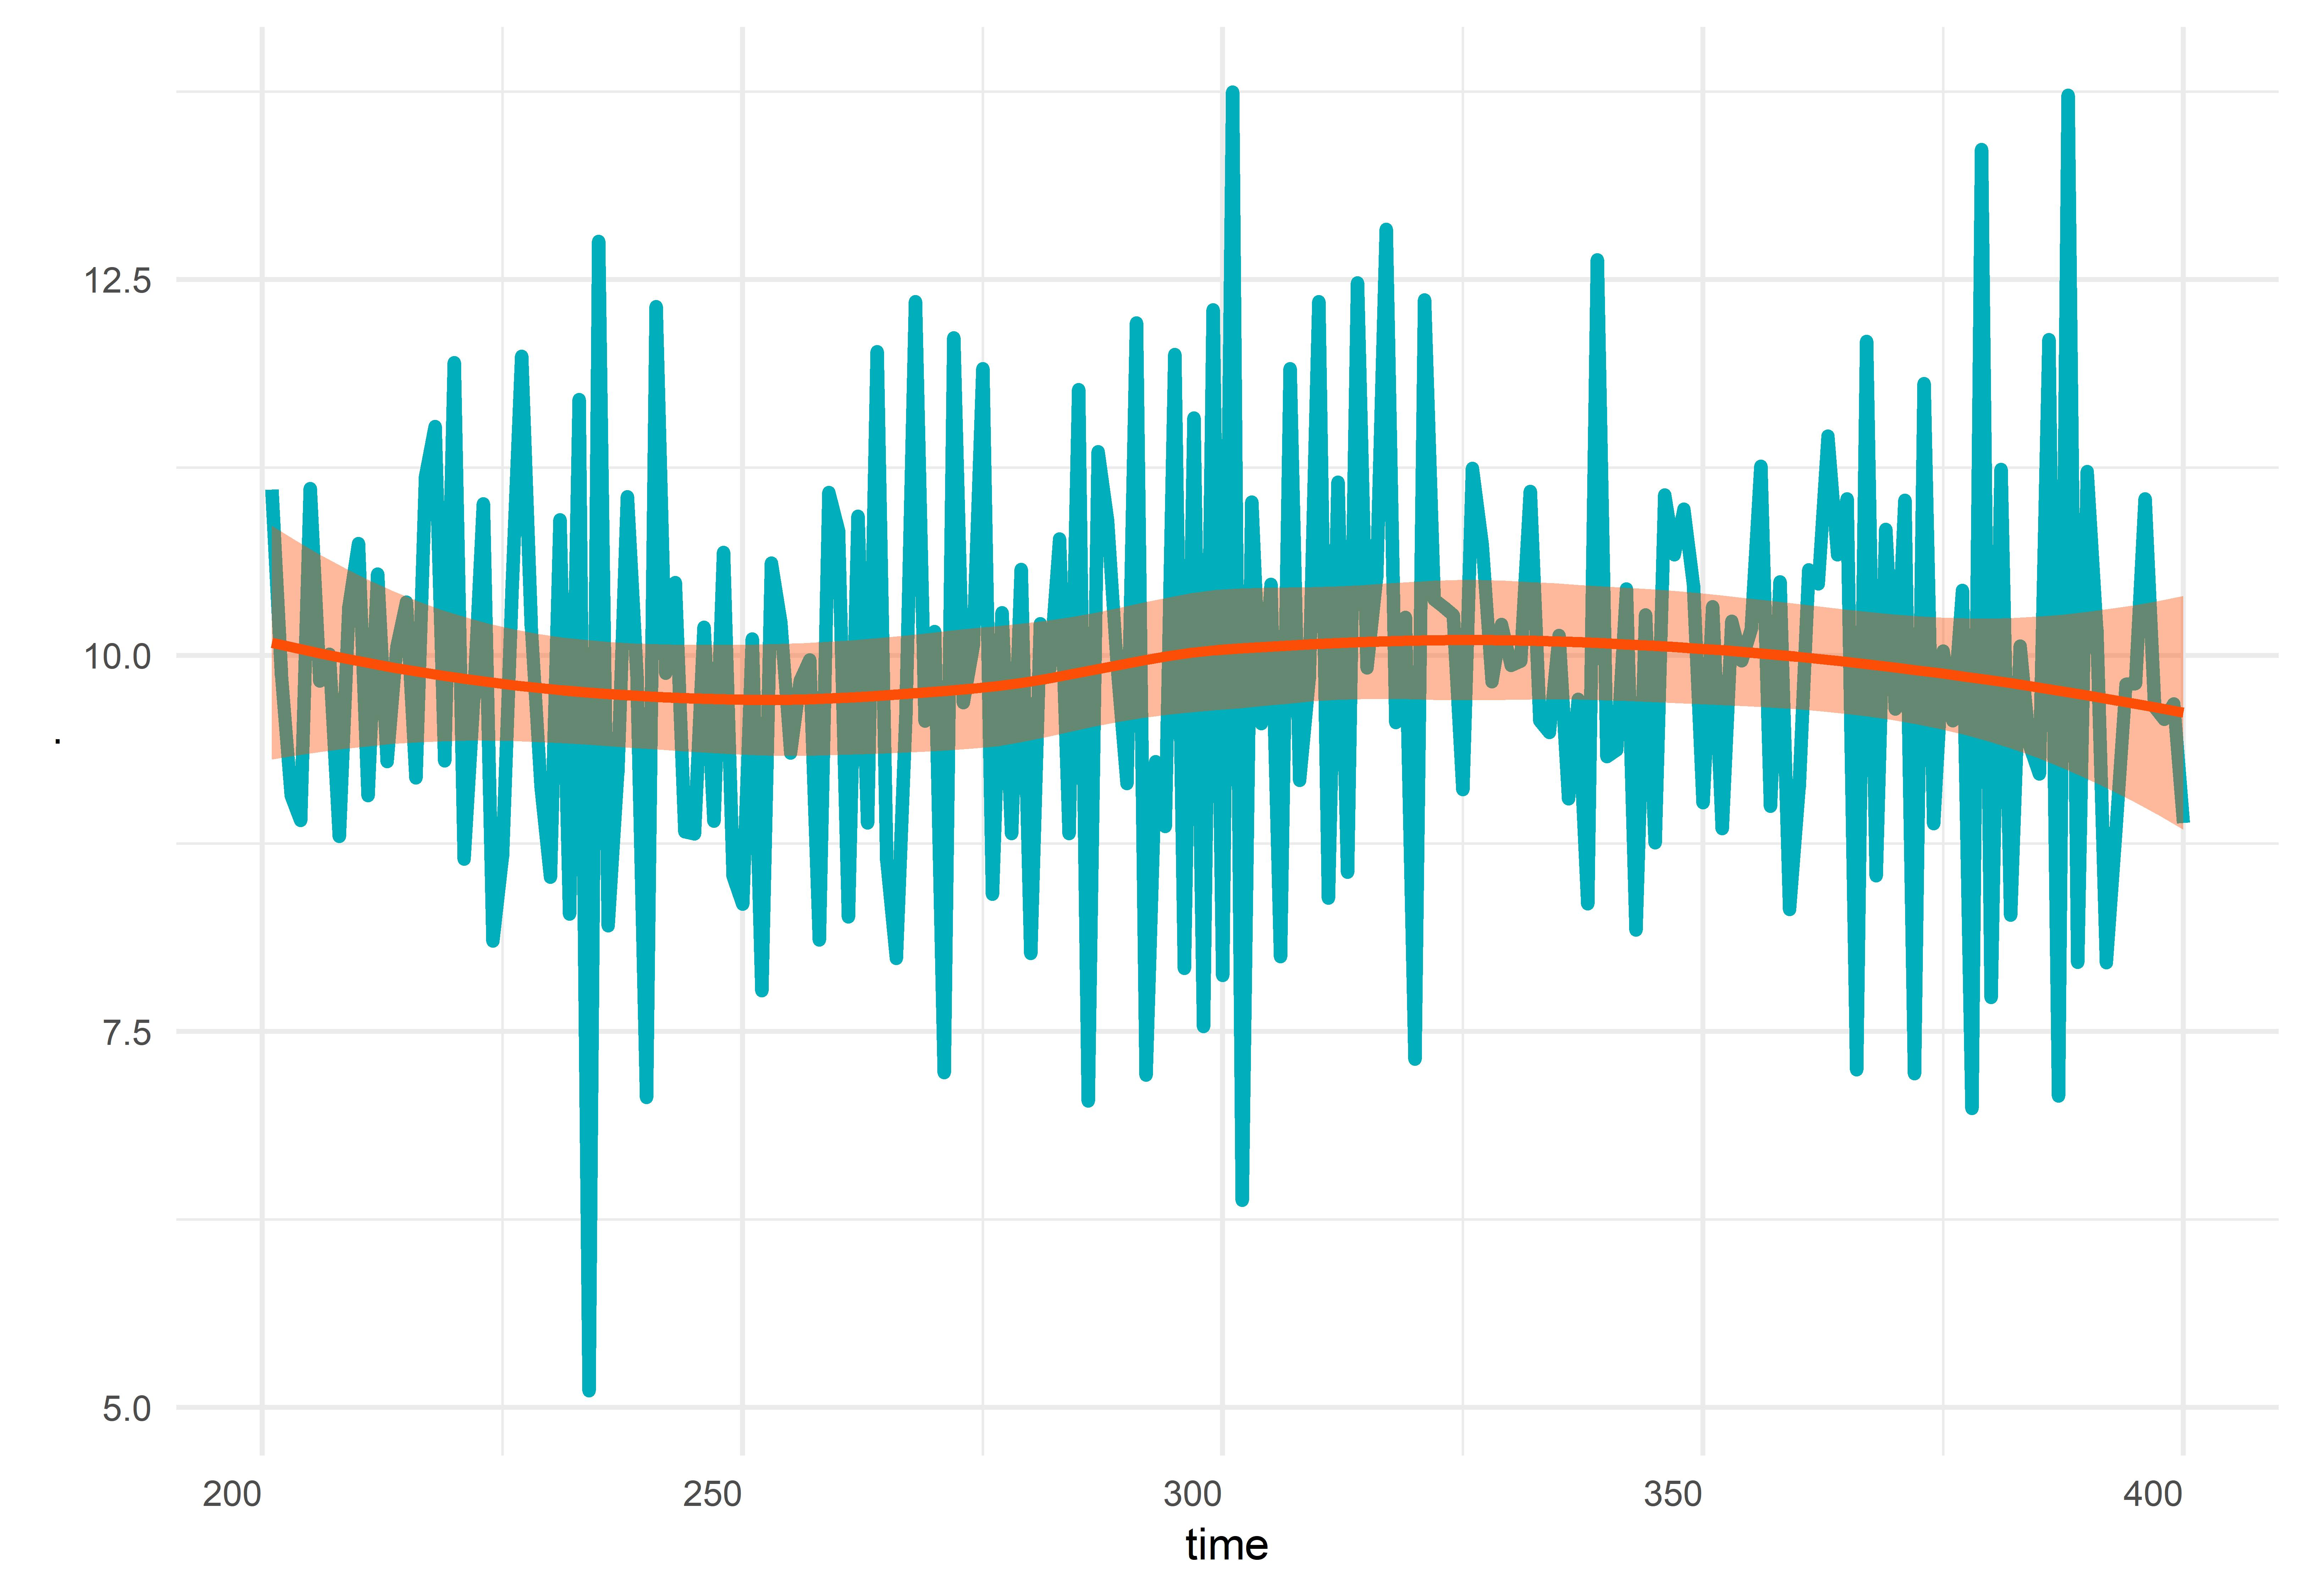
\includegraphics[width=1\linewidth,height=1\textheight]{Tesis_files/figure-latex/arima100_comportamiento-1} \caption{Tendencia de los datos simulados a partir de un proceso ARIMA(1,0,0)}\label{fig:arima100_comportamiento}
\end{figure}

\begin{figure}[H]
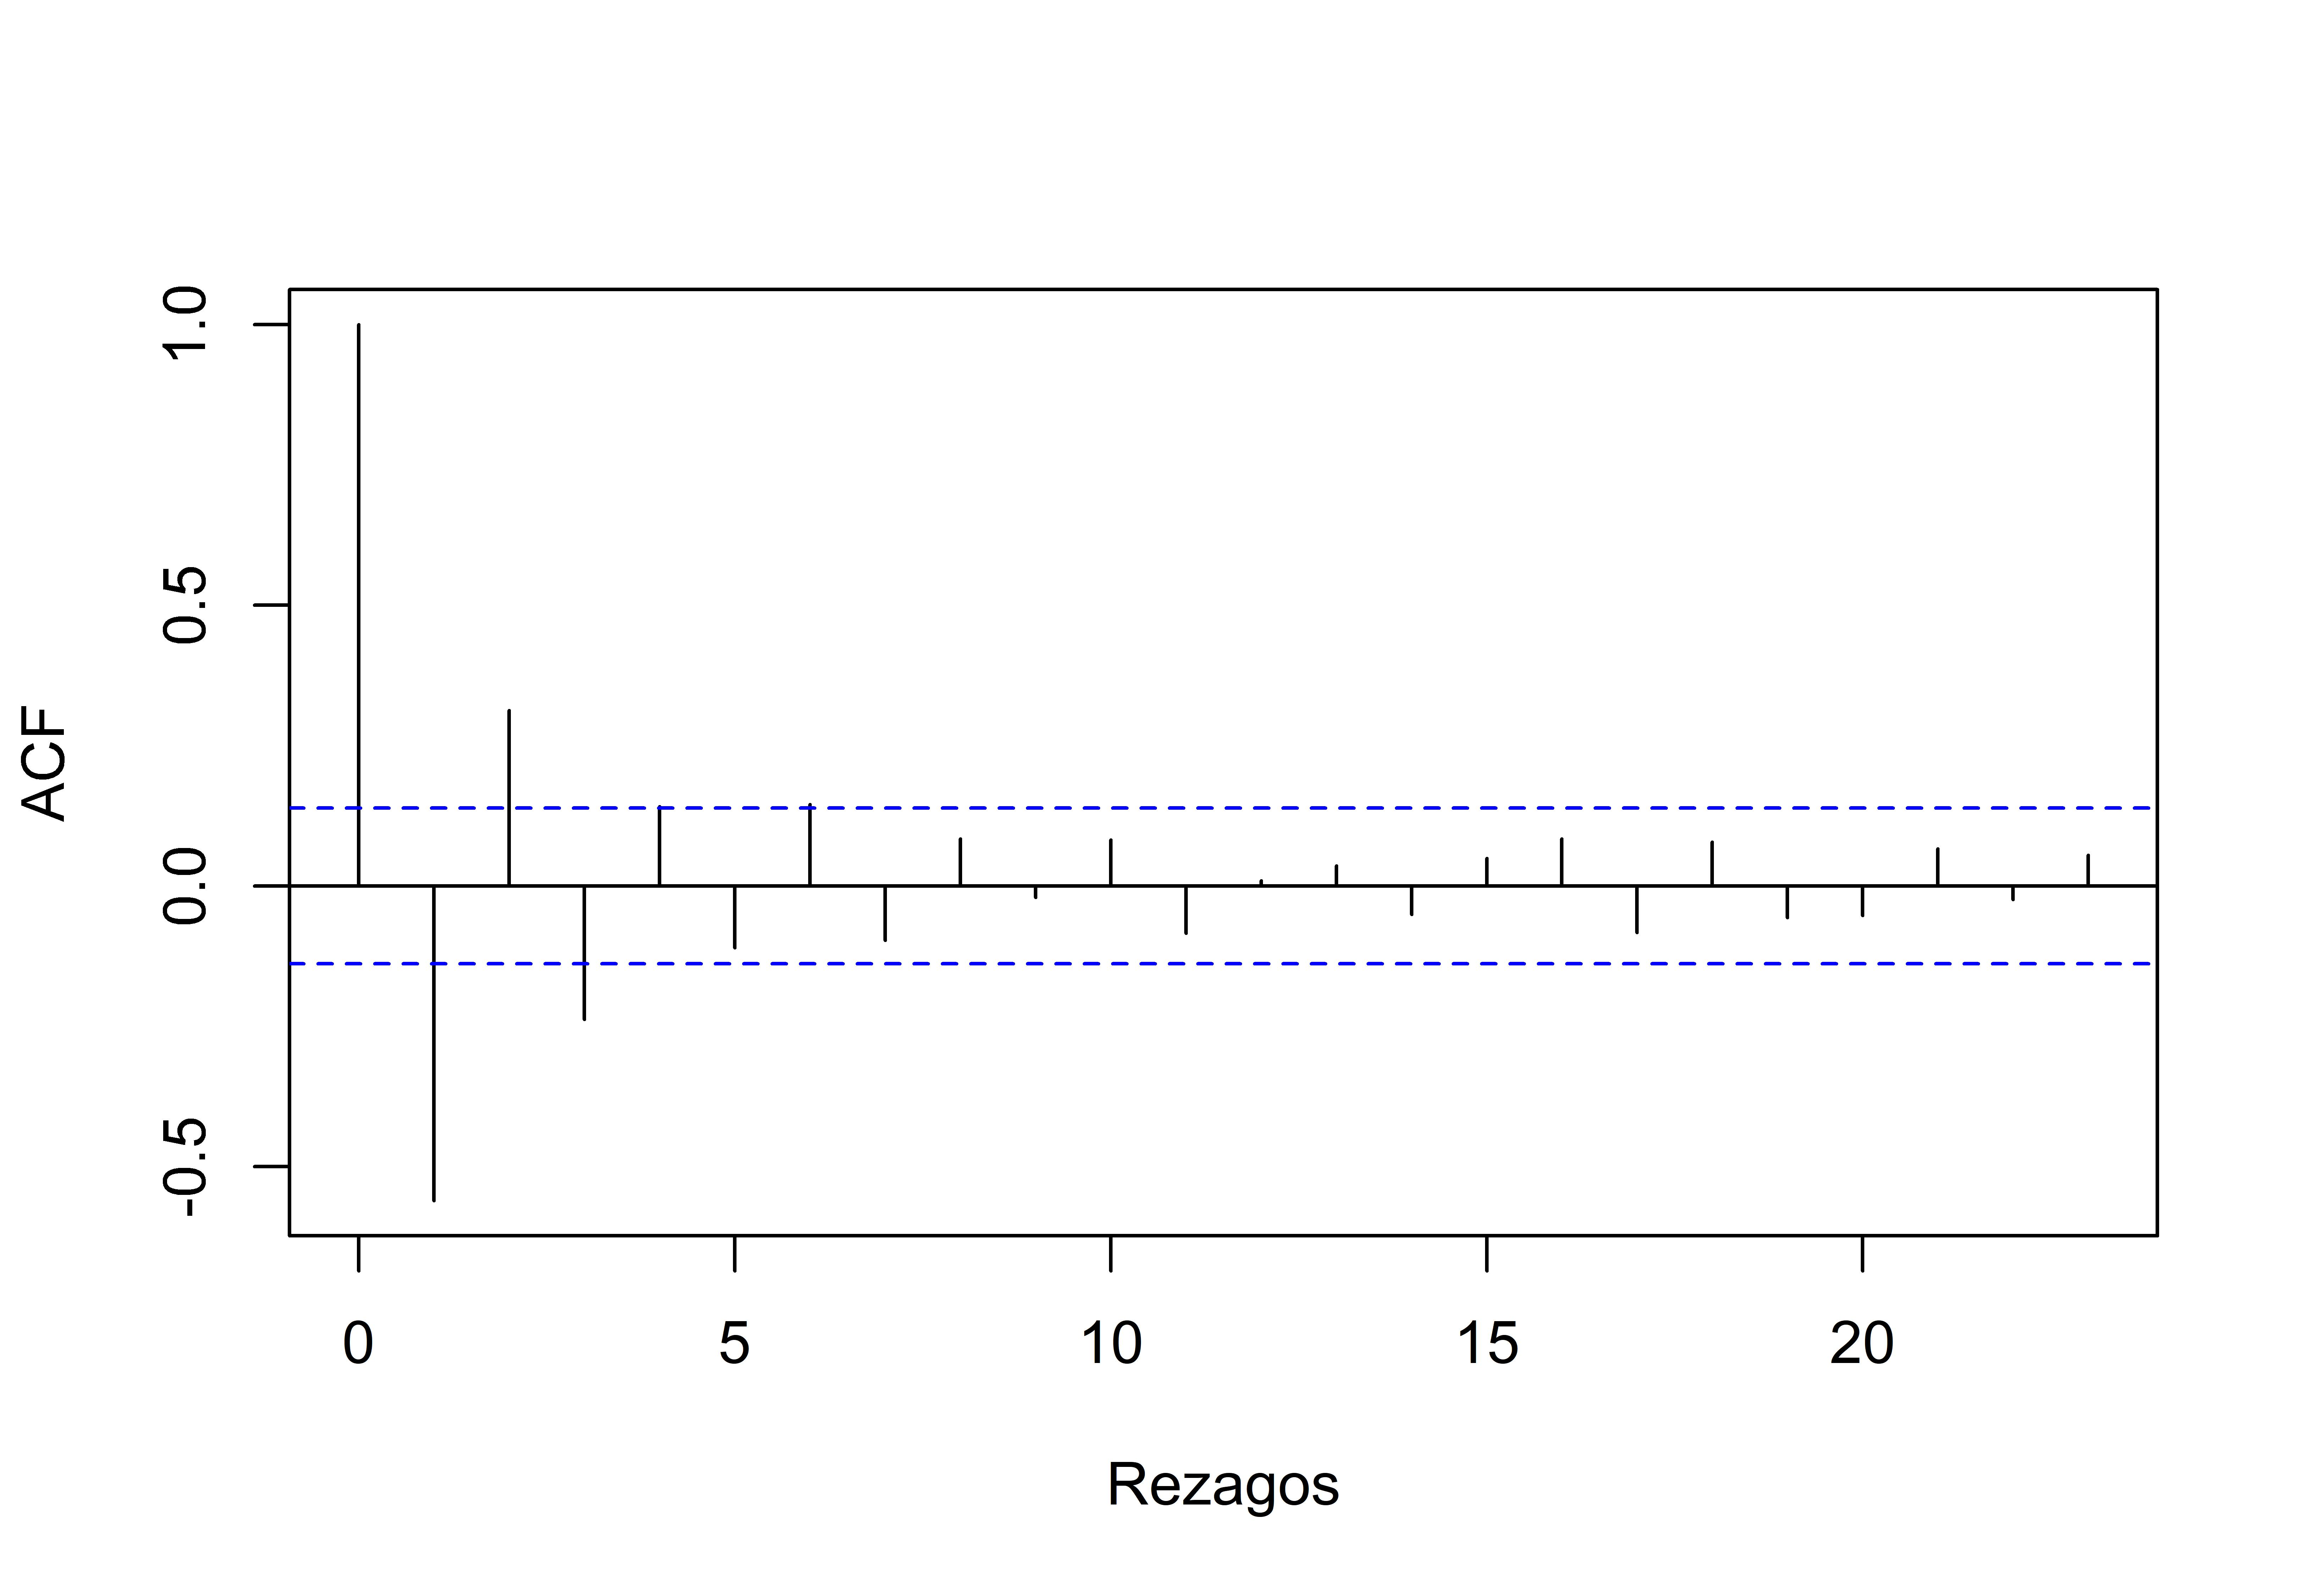
\includegraphics[width=1\linewidth,height=1\textheight]{Tesis_files/figure-latex/arima100_acf-1} \caption{Autocorrelación de los datos simulados a partir de un proceso ARIMA(1,0,0)}\label{fig:arima100_acf}
\end{figure}

\begin{figure}[H]
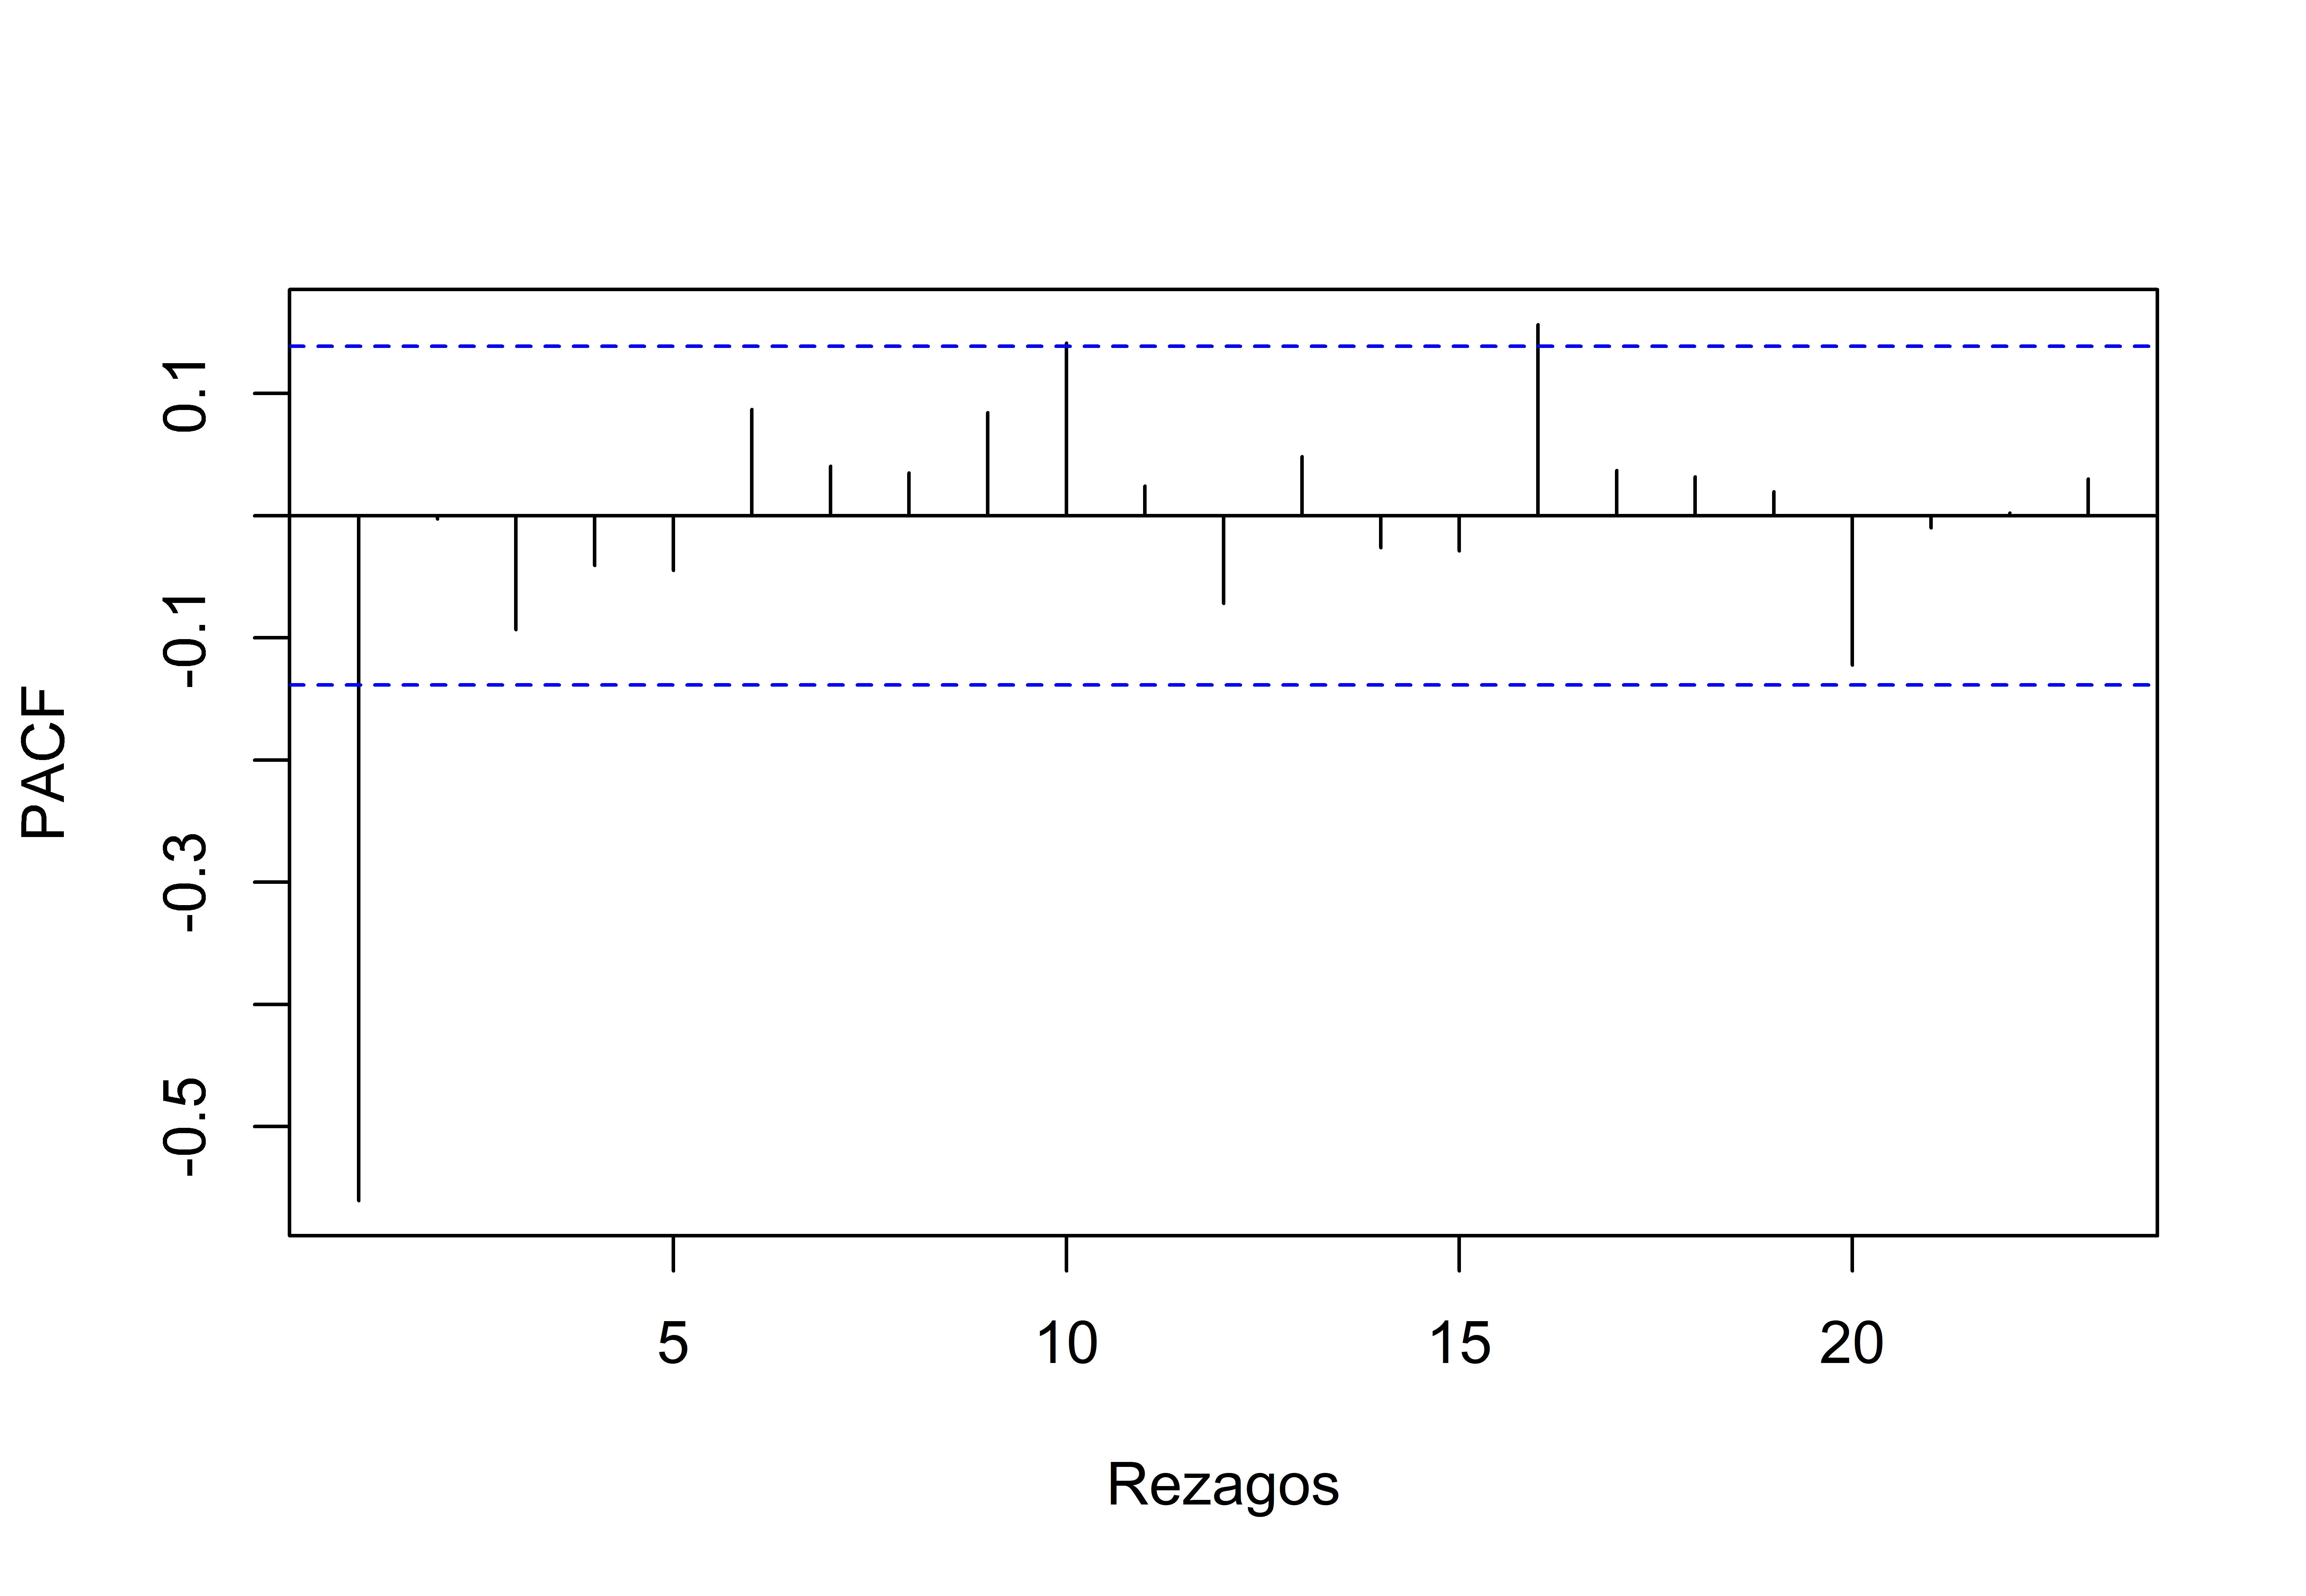
\includegraphics[width=1\linewidth,height=1\textheight]{Tesis_files/figure-latex/arima100_pacf-1} \caption{Autocorrelación parcial de los datos simulados a partir de un proceso ARIMA(1,0,0)}\label{fig:arima100_pacf}
\end{figure}

\paragraph{ARIMA(1,0,1)}

En la figura \ref{fig:arima101_comportamiento} puede verse como los
datos simulados bajo este proceso se comportan de manera más oscilante
que el caso anterior a lo largo del tiempo. Además, la figura
\ref{fig:arima101_acf} muestra como las autocorrelaciones van
disminuyendo muy lentamente, mientras que se aprecia en la figura
\ref{fig:arima101_pacf} que hay un comportamiento similar al caso
anterior, pues también va disminuyendo, lo que sugiere que el posible
proceso que gobierna los datos podría tratarse de un \(ARIMA(1,0,1)\),
tal y como fue planteado al simular los datos.

\begin{figure}[H]
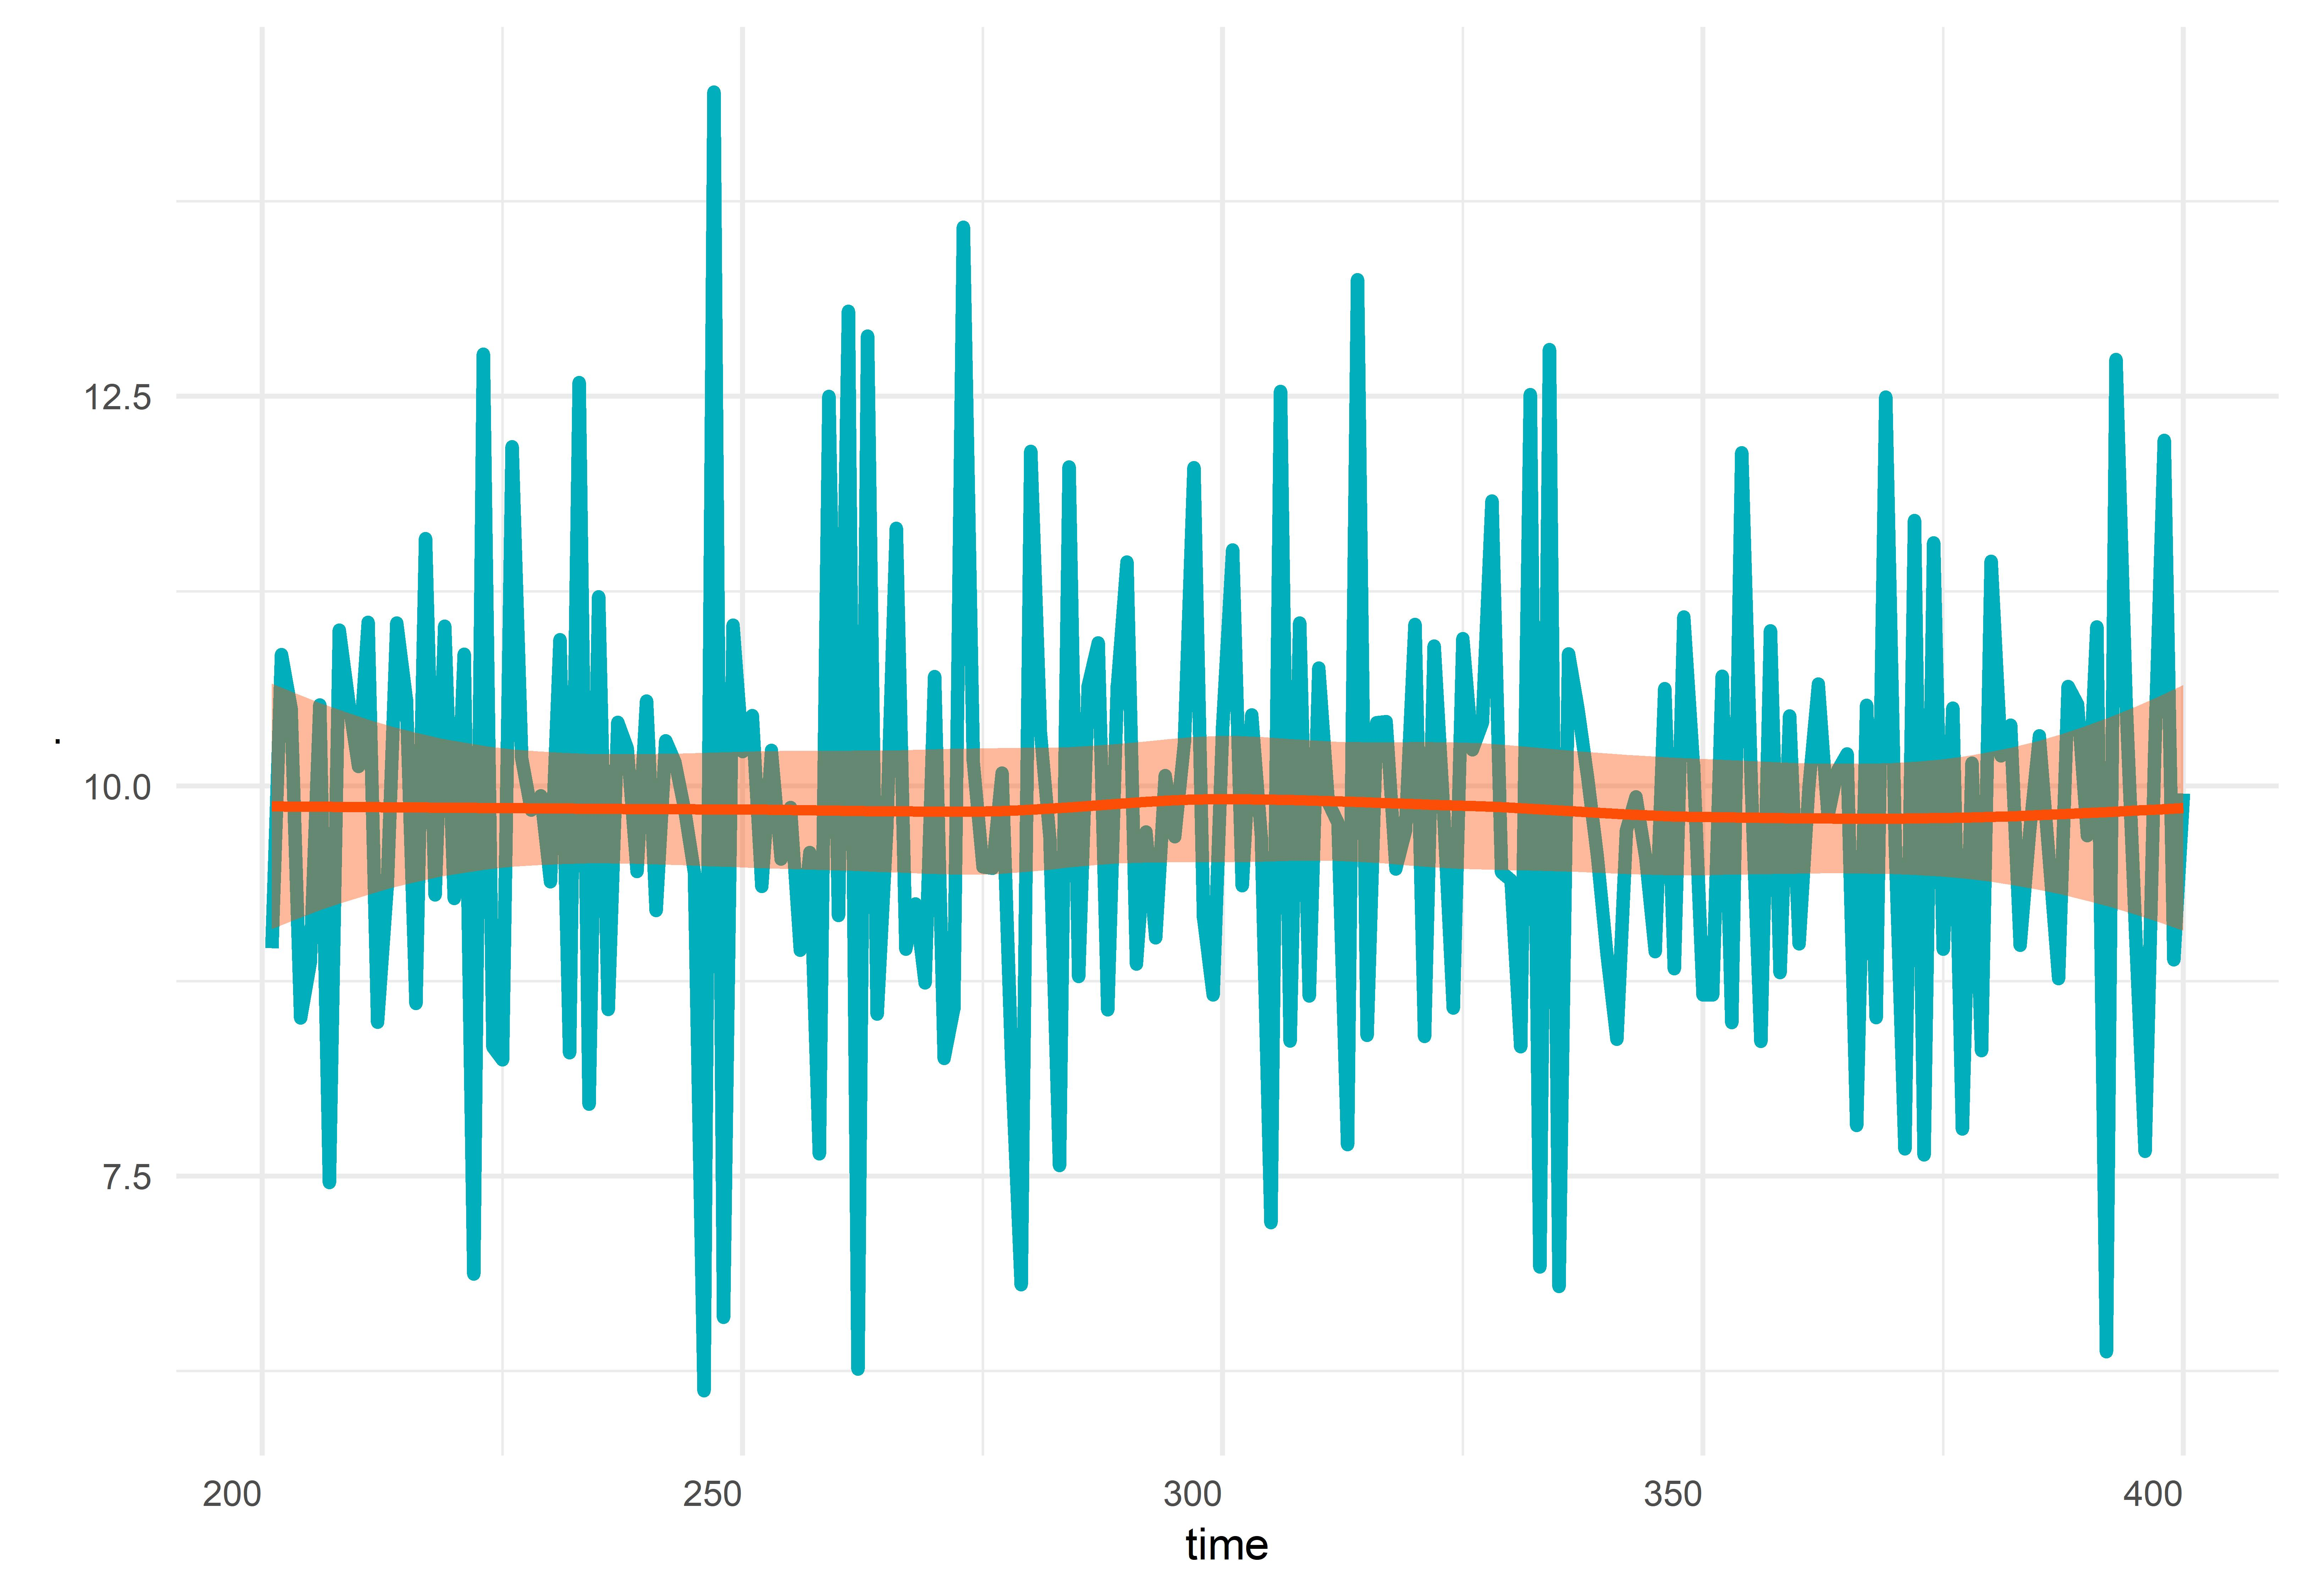
\includegraphics[width=1\linewidth,height=1\textheight]{Tesis_files/figure-latex/arima101_comportamiento-1} \caption{Tendencia de los datos simulados a partir de un proceso ARIMA(1,0,1)}\label{fig:arima101_comportamiento}
\end{figure}

\begin{figure}[H]
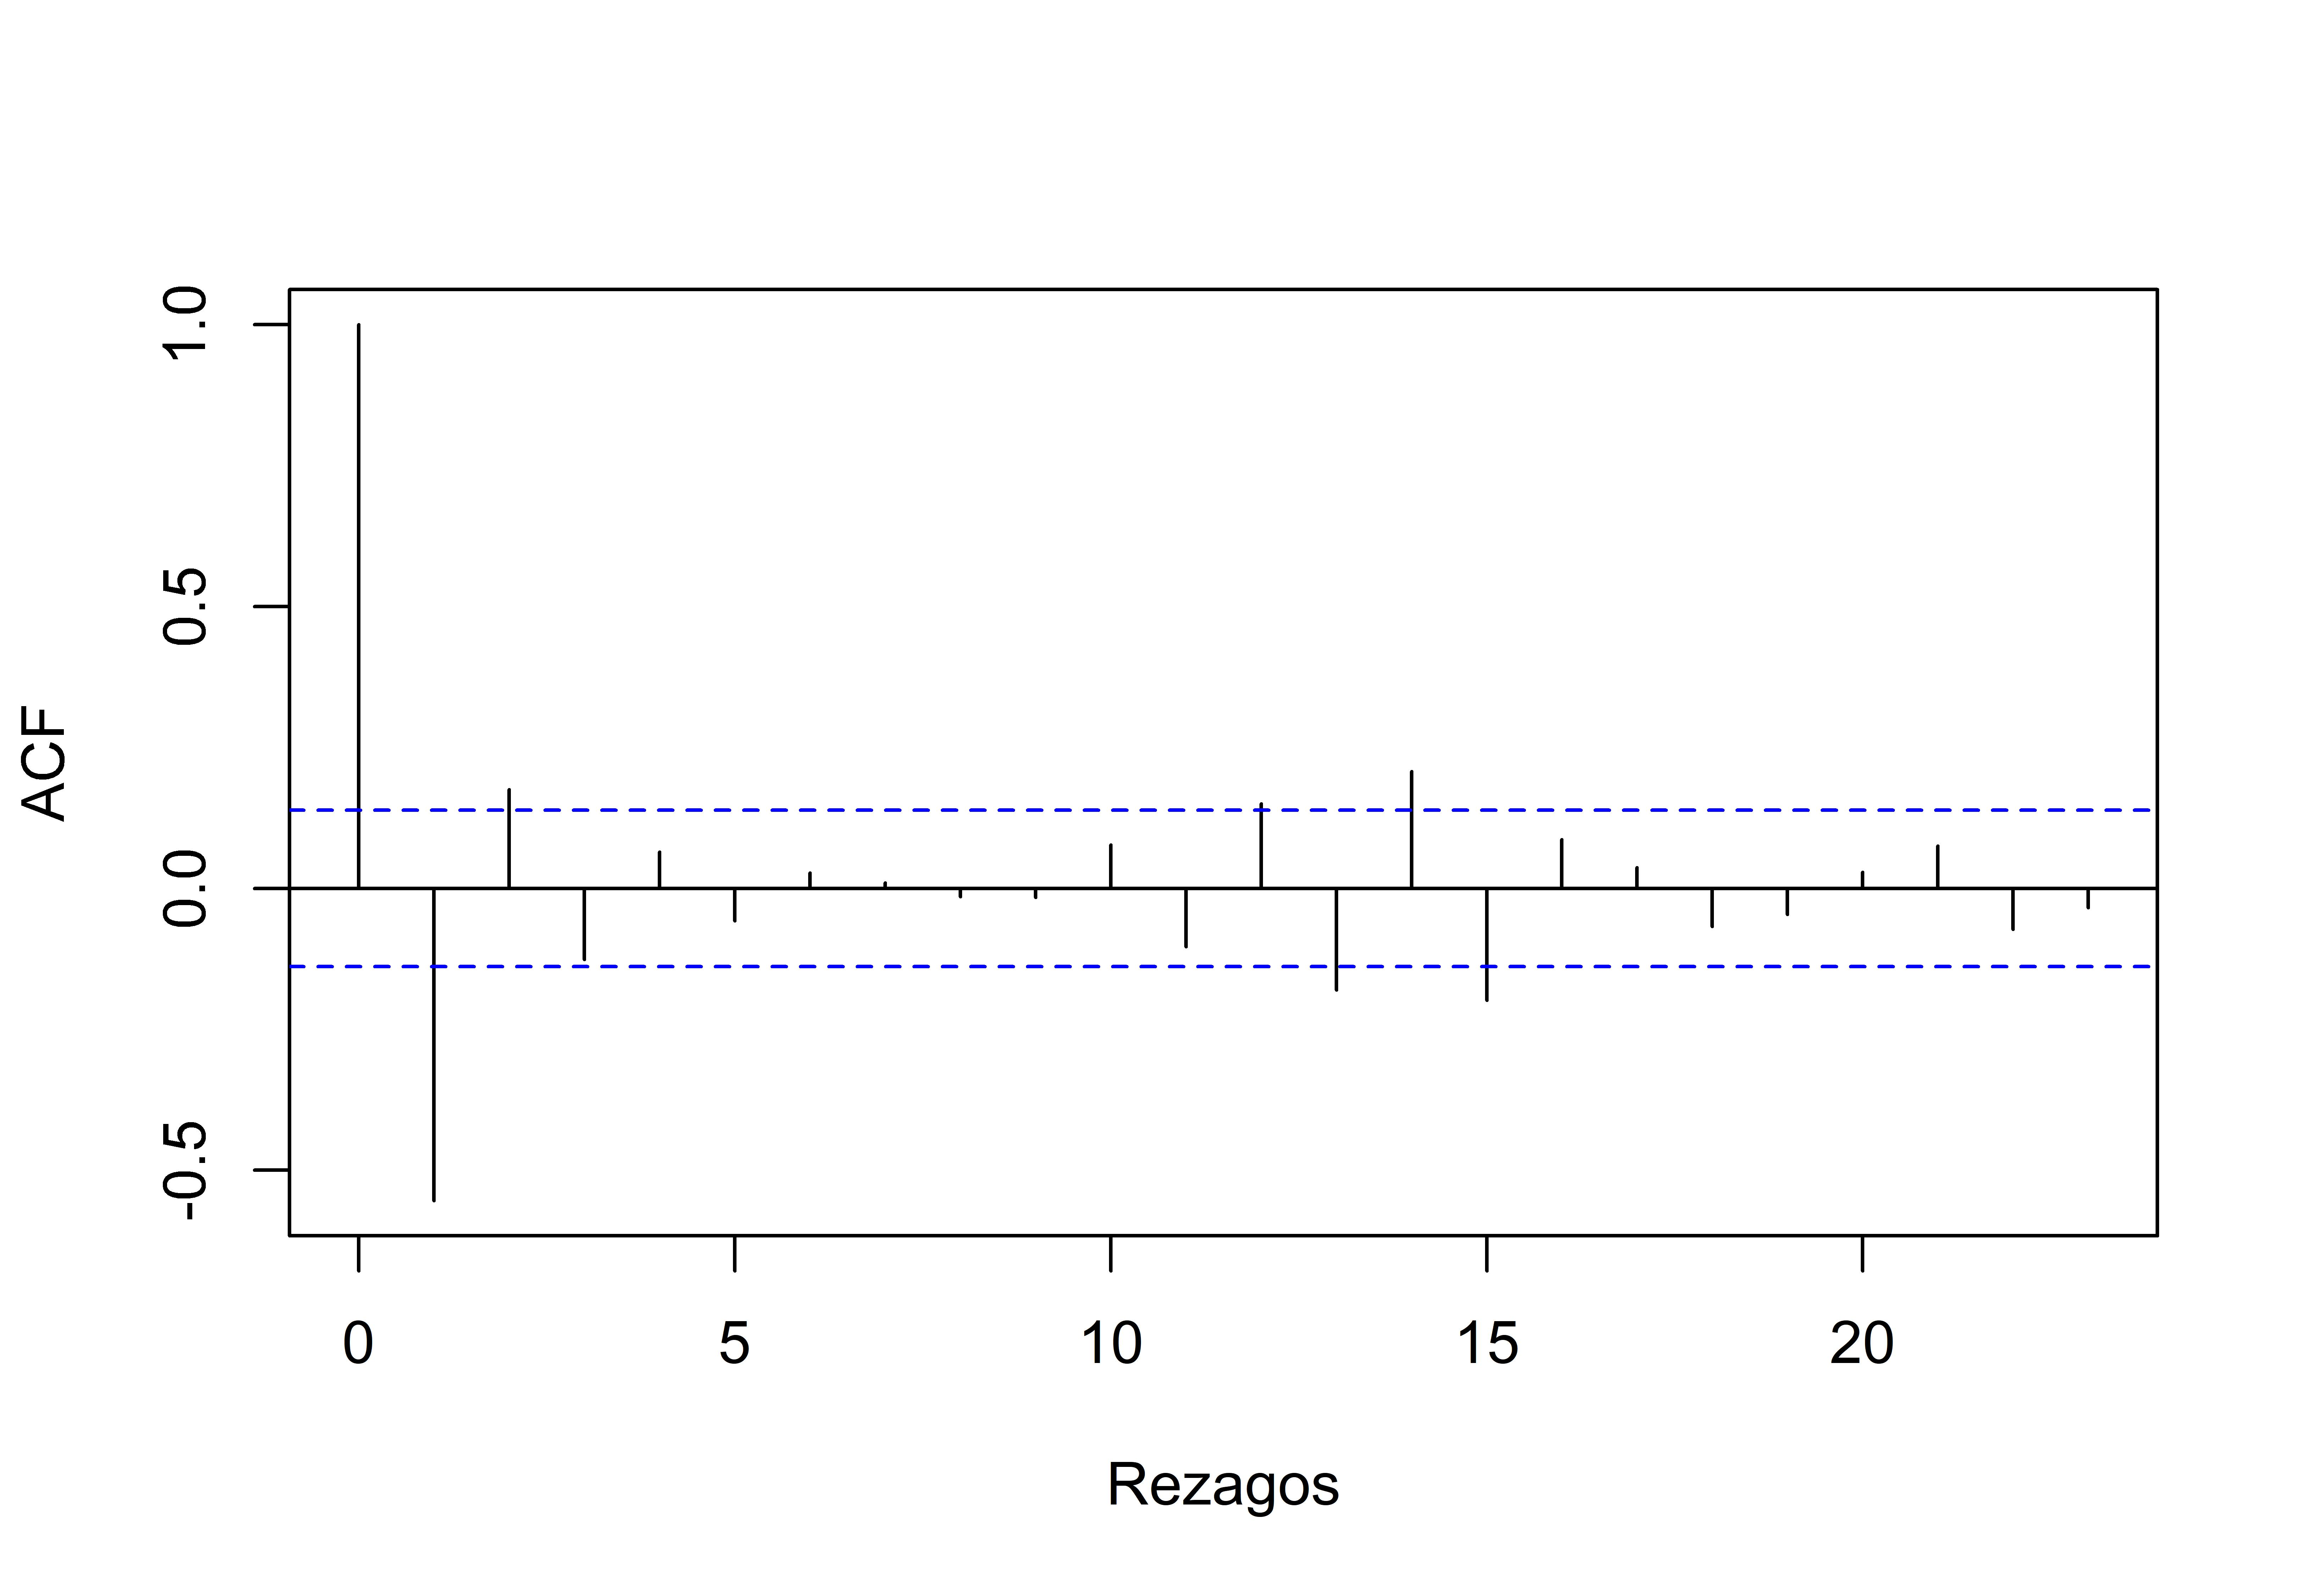
\includegraphics[width=1\linewidth,height=1\textheight]{Tesis_files/figure-latex/arima101_acf-1} \caption{Autocorrelación de los datos simulados a partir de un proceso ARIMA(1,0,1)}\label{fig:arima101_acf}
\end{figure}

\begin{figure}[H]
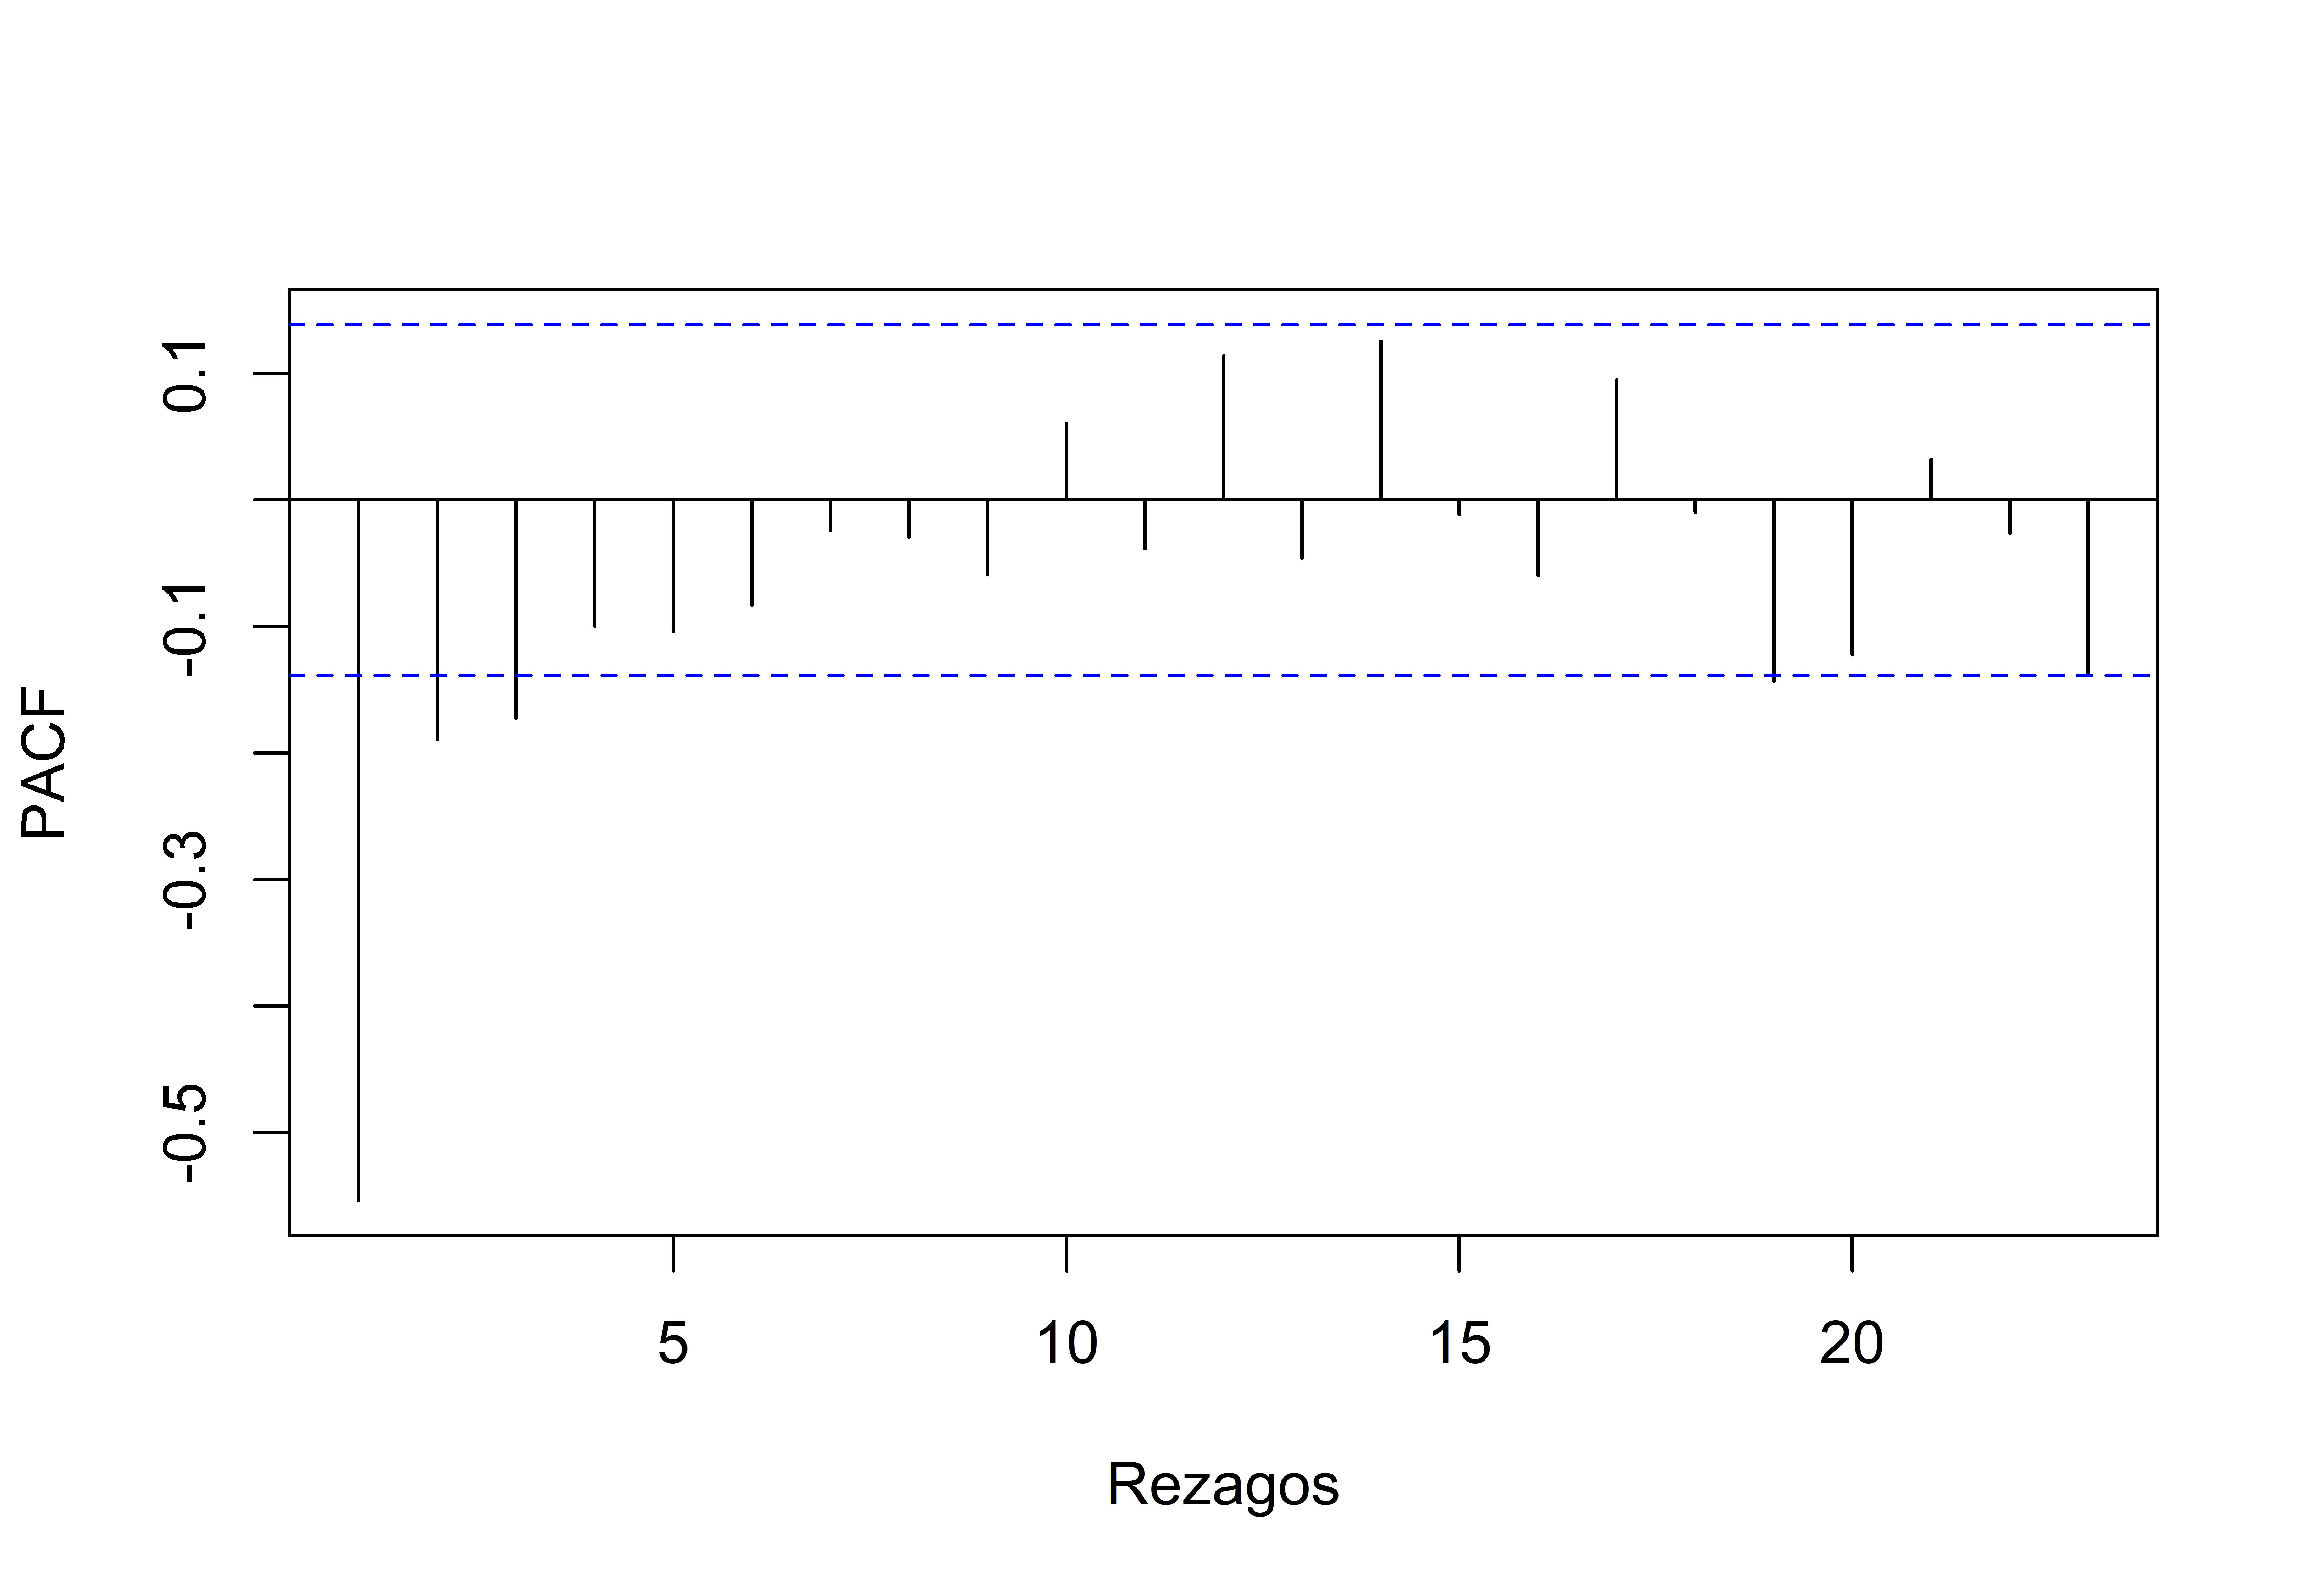
\includegraphics[width=1\linewidth,height=1\textheight]{Tesis_files/figure-latex/arima101_pacf-1} \caption{Autocorrelación parcial de los datos simulados a partir de un proceso ARIMA(1,0,1)}\label{fig:arima101_pacf}
\end{figure}

\paragraph{ARIMA(2,0,3)}

En la figura \ref{fig:arima203_comportamiento} se observa como los datos
simulados bajo este proceso no parecen tener ninguna tendencia clara,
una alternativa en este caso sería aplicar alguna transformación para
volverla aún más estacionaria. La figura \ref{fig:arima203_acf} muestra
como las autocorrelaciones van disminuyendo, situación no tan clara en
la figura \ref{fig:arima203_pacf}, este escenario sugiere que se está en
presencia de un proceso \(ARMA(p,q)\), por lo que podrían ajustarse
varios modelos \(ARIMA(p,d,q)\) hasta encontrar el más adecuado.

\begin{figure}[H]
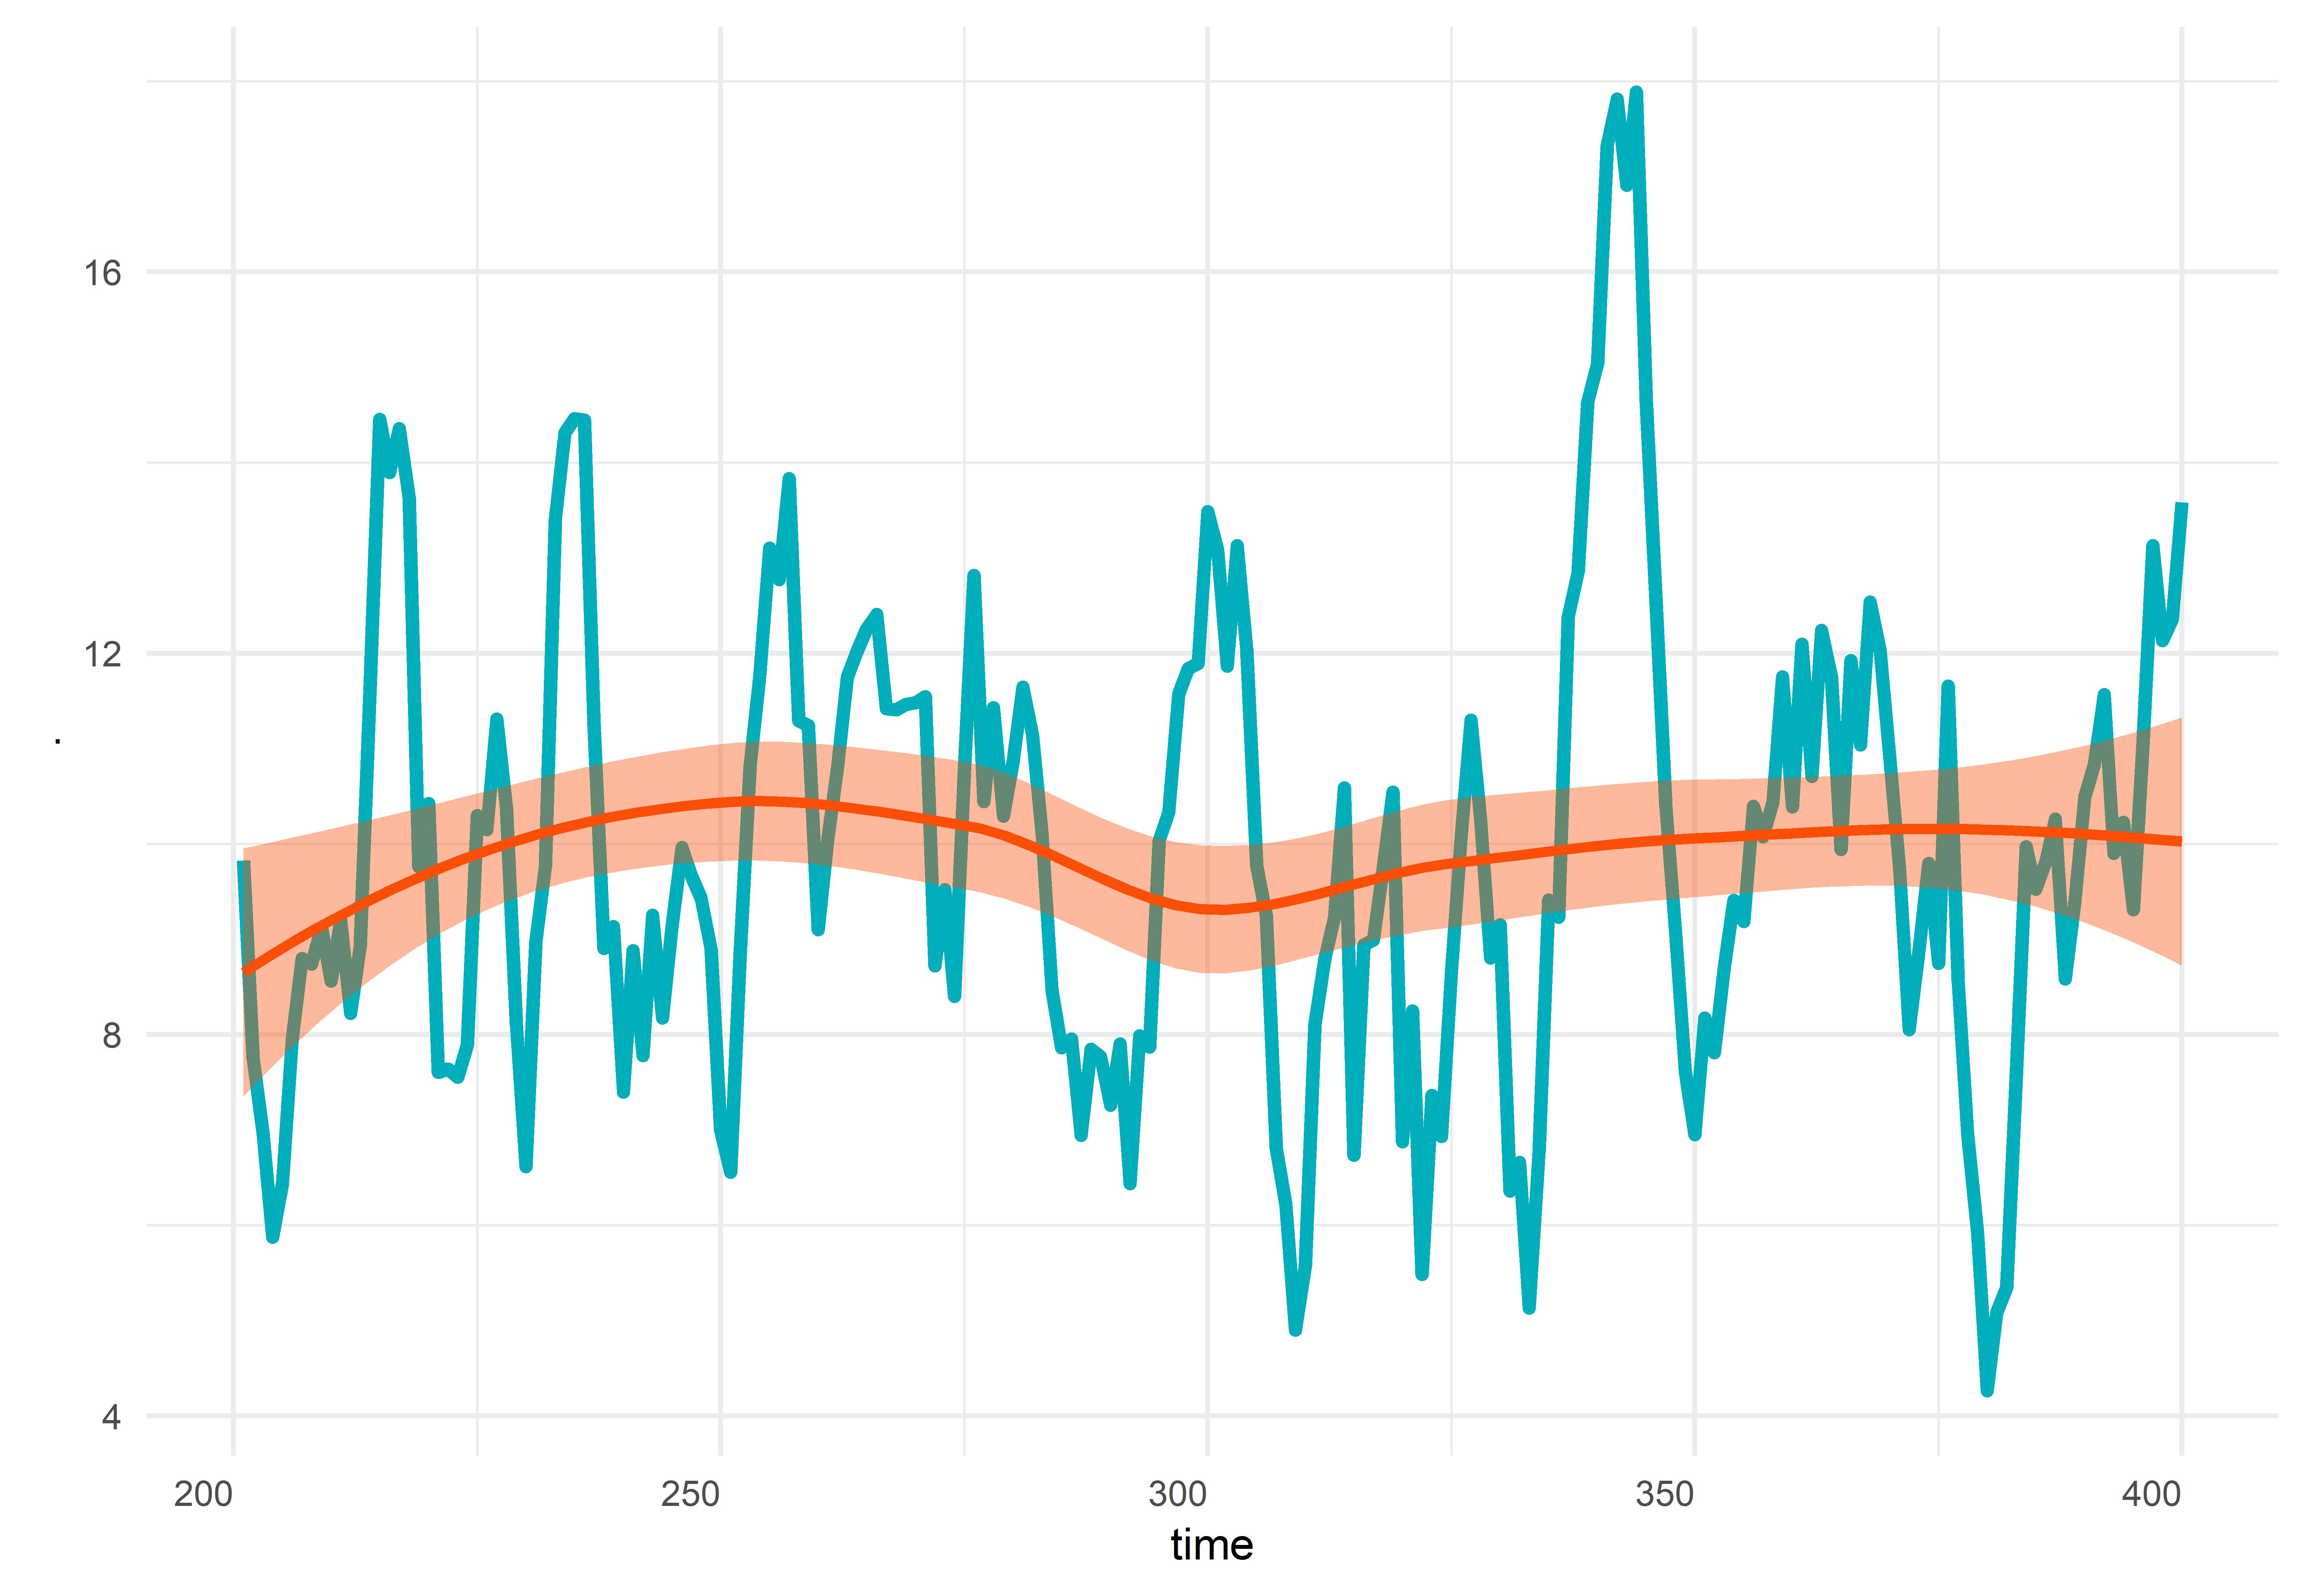
\includegraphics[width=1\linewidth,height=1\textheight]{Tesis_files/figure-latex/arima203_comportamiento-1} \caption{Tendencia de los datos simulados a partir de un proceso ARIMA(2,0,3)}\label{fig:arima203_comportamiento}
\end{figure}

\begin{figure}[H]
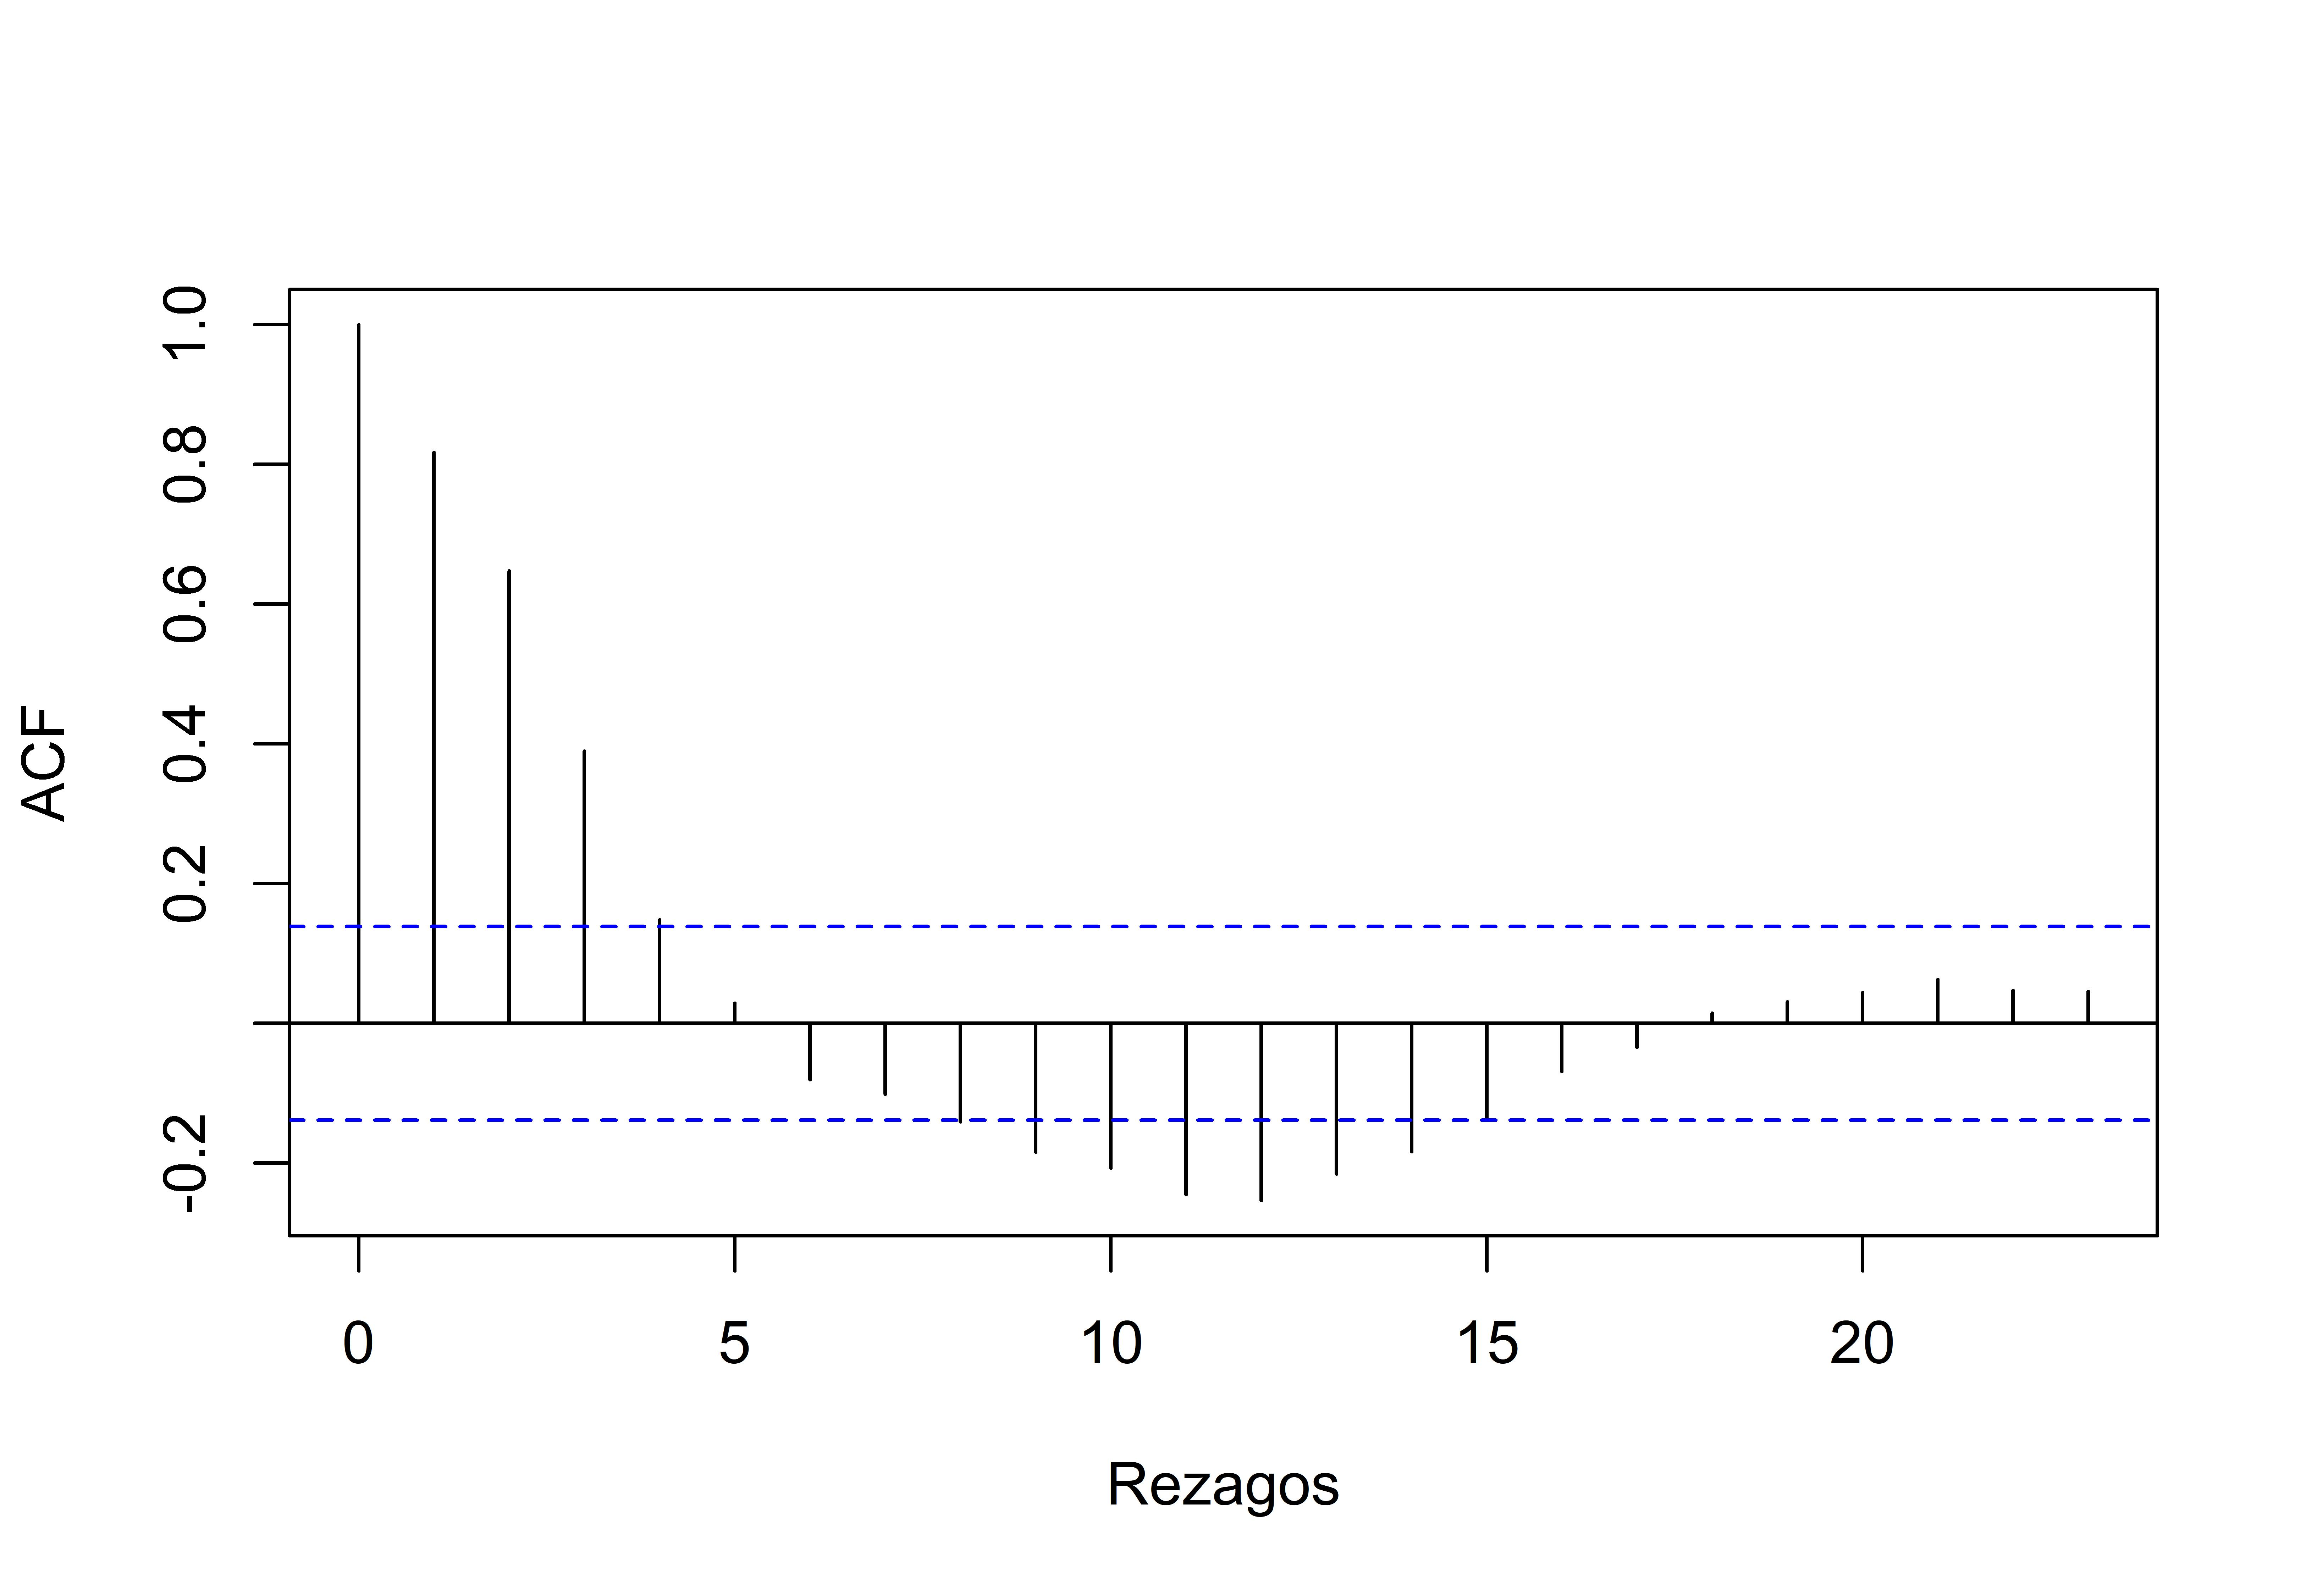
\includegraphics[width=1\linewidth,height=1\textheight]{Tesis_files/figure-latex/arima203_acf-1} \caption{Autocorrelación de los datos simulados a partir de un proceso ARIMA(2,0,3)}\label{fig:arima203_acf}
\end{figure}

\begin{figure}[H]
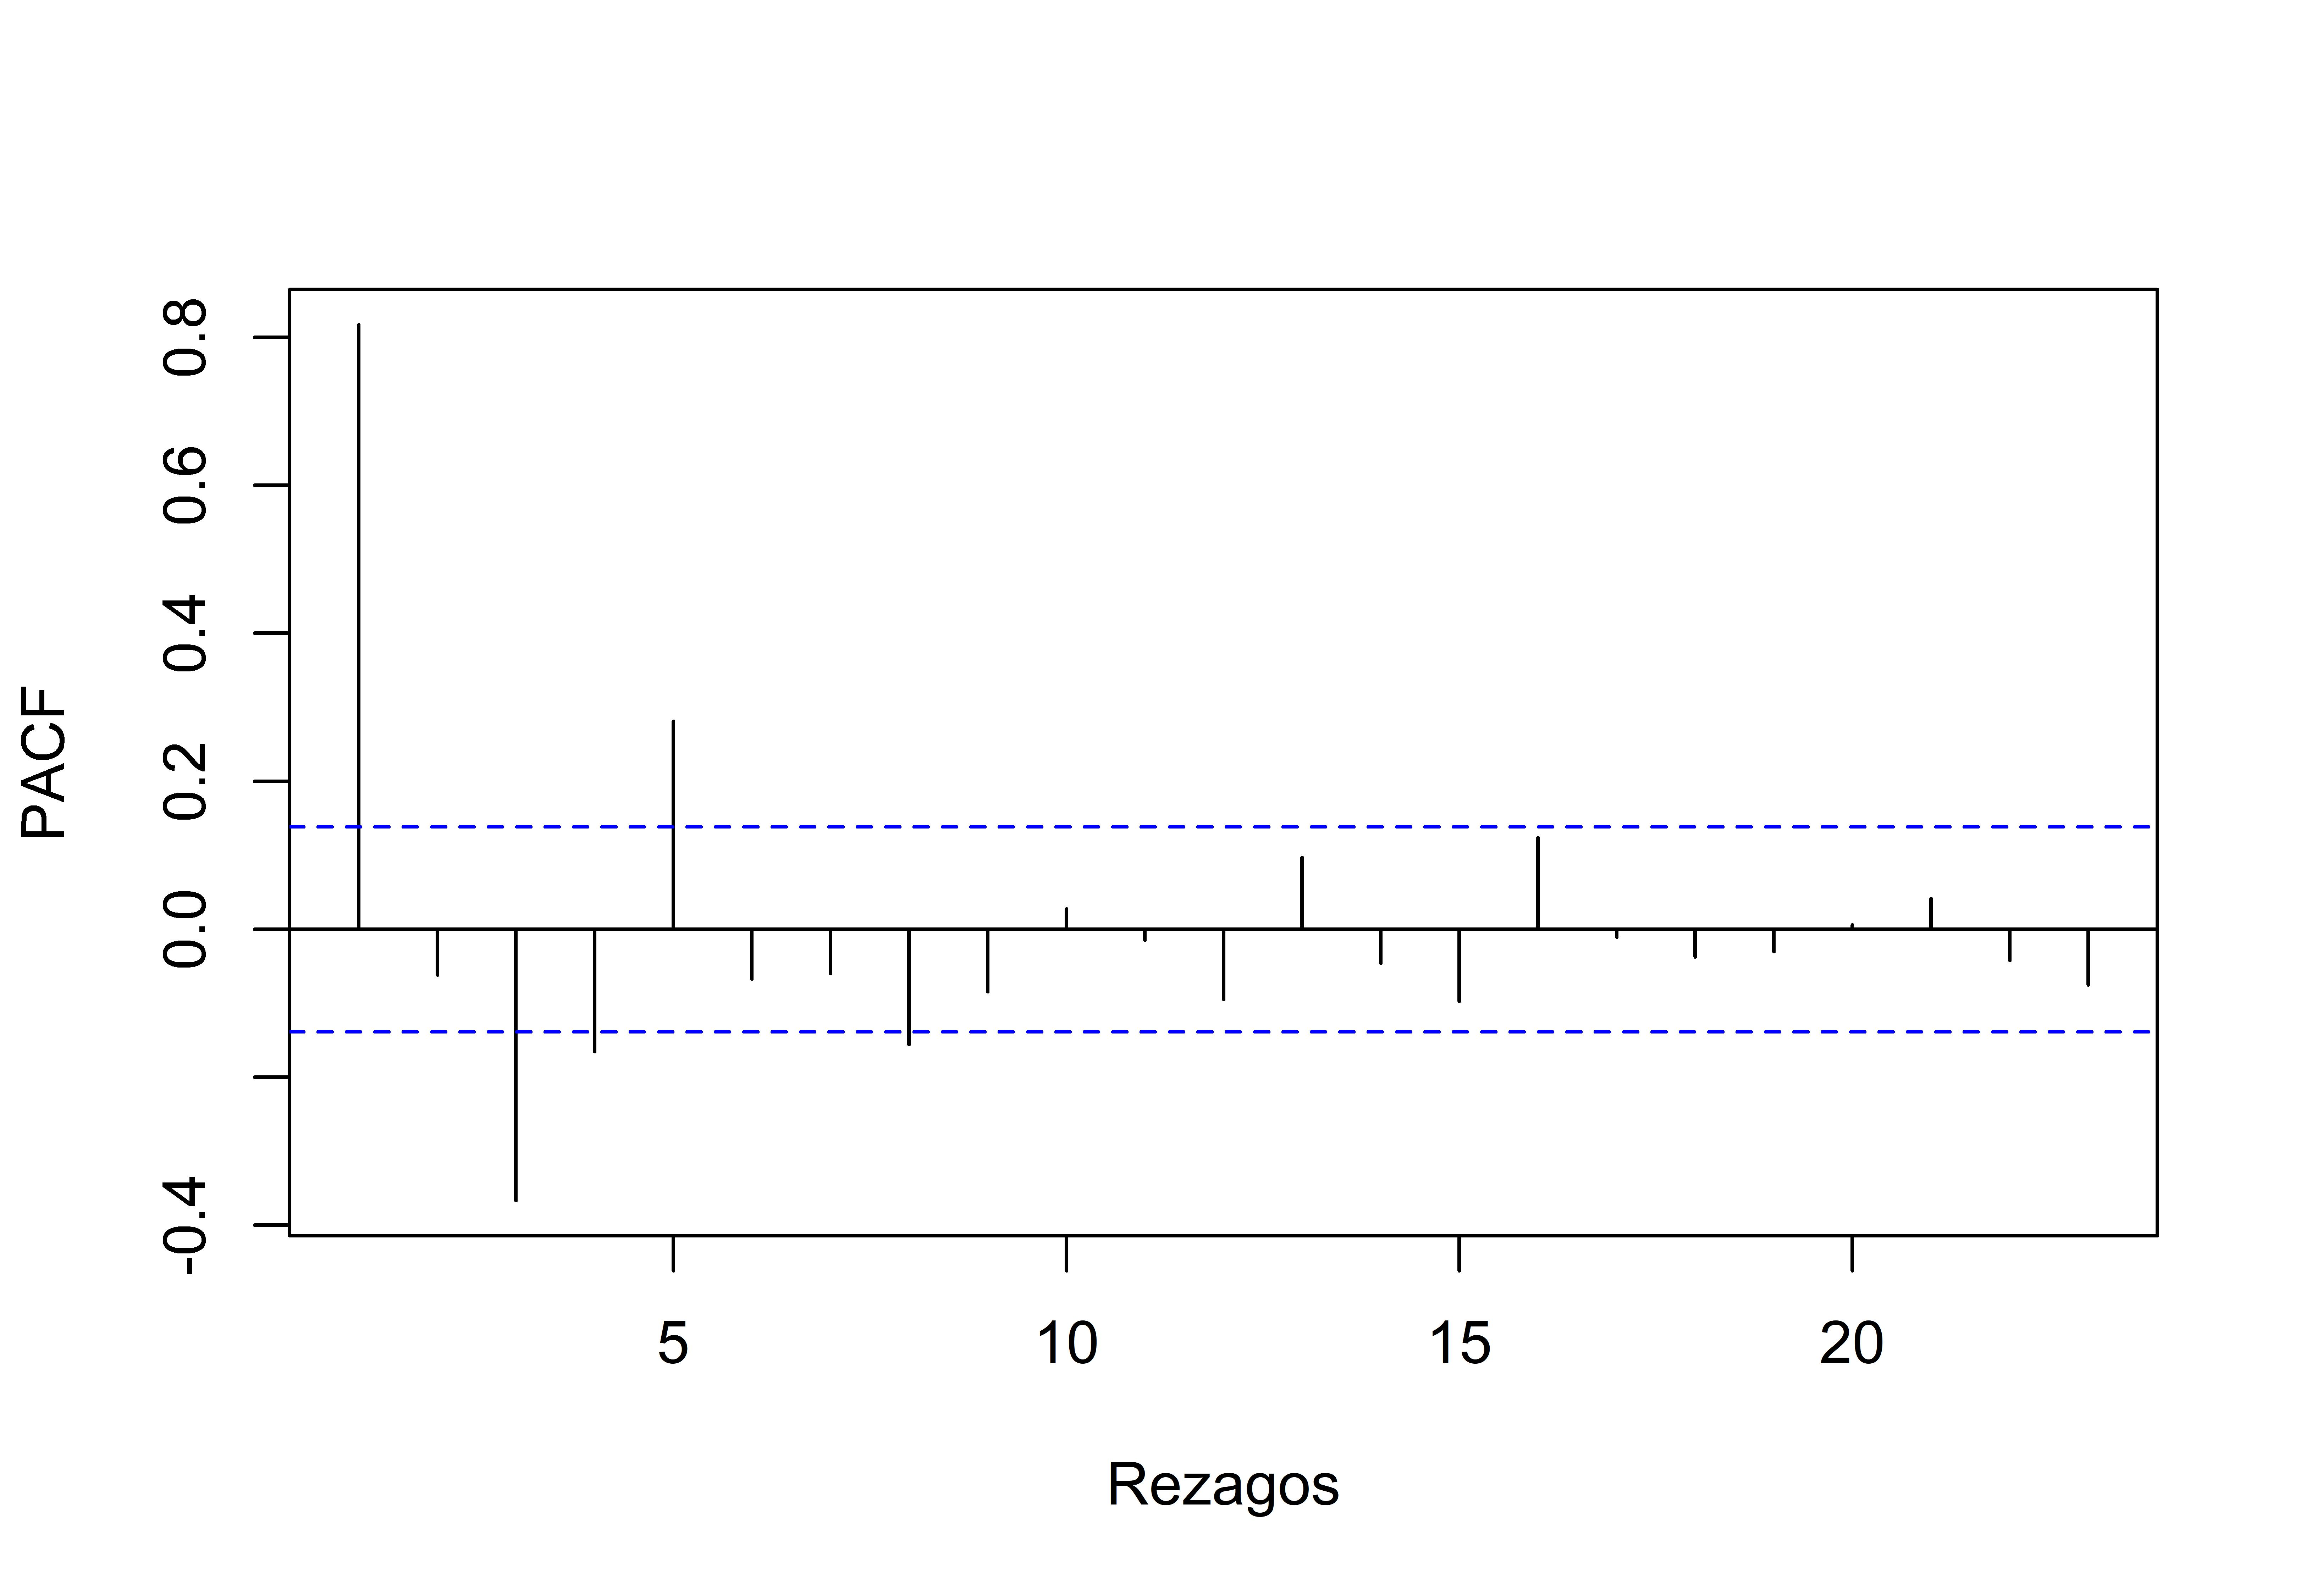
\includegraphics[width=1\linewidth,height=1\textheight]{Tesis_files/figure-latex/arima203_pacf-1} \caption{Autocorrelación parcial de los datos simulados a partir de un proceso ARIMA(2,0,3)}\label{fig:arima203_pacf}
\end{figure}

\paragraph{ARIMA(4,0,2)}

En la figura \ref{fig:arima402_comportamiento} se observa como los datos
simulados bajo este proceso tampoco parecen tener una tendencia
claramente definida, por lo que podría ser necesario aplicar alguna
transformación. Las figuras \ref{fig:arima402_acf} y
\ref{fig:arima402_pacf} presentan una situación similar a la anterior,
por lo que podrían ajustarse varios modelos \(ARIMA(p,d,q)\) hasta
encontrar el más adecuado.

\begin{figure}[H]
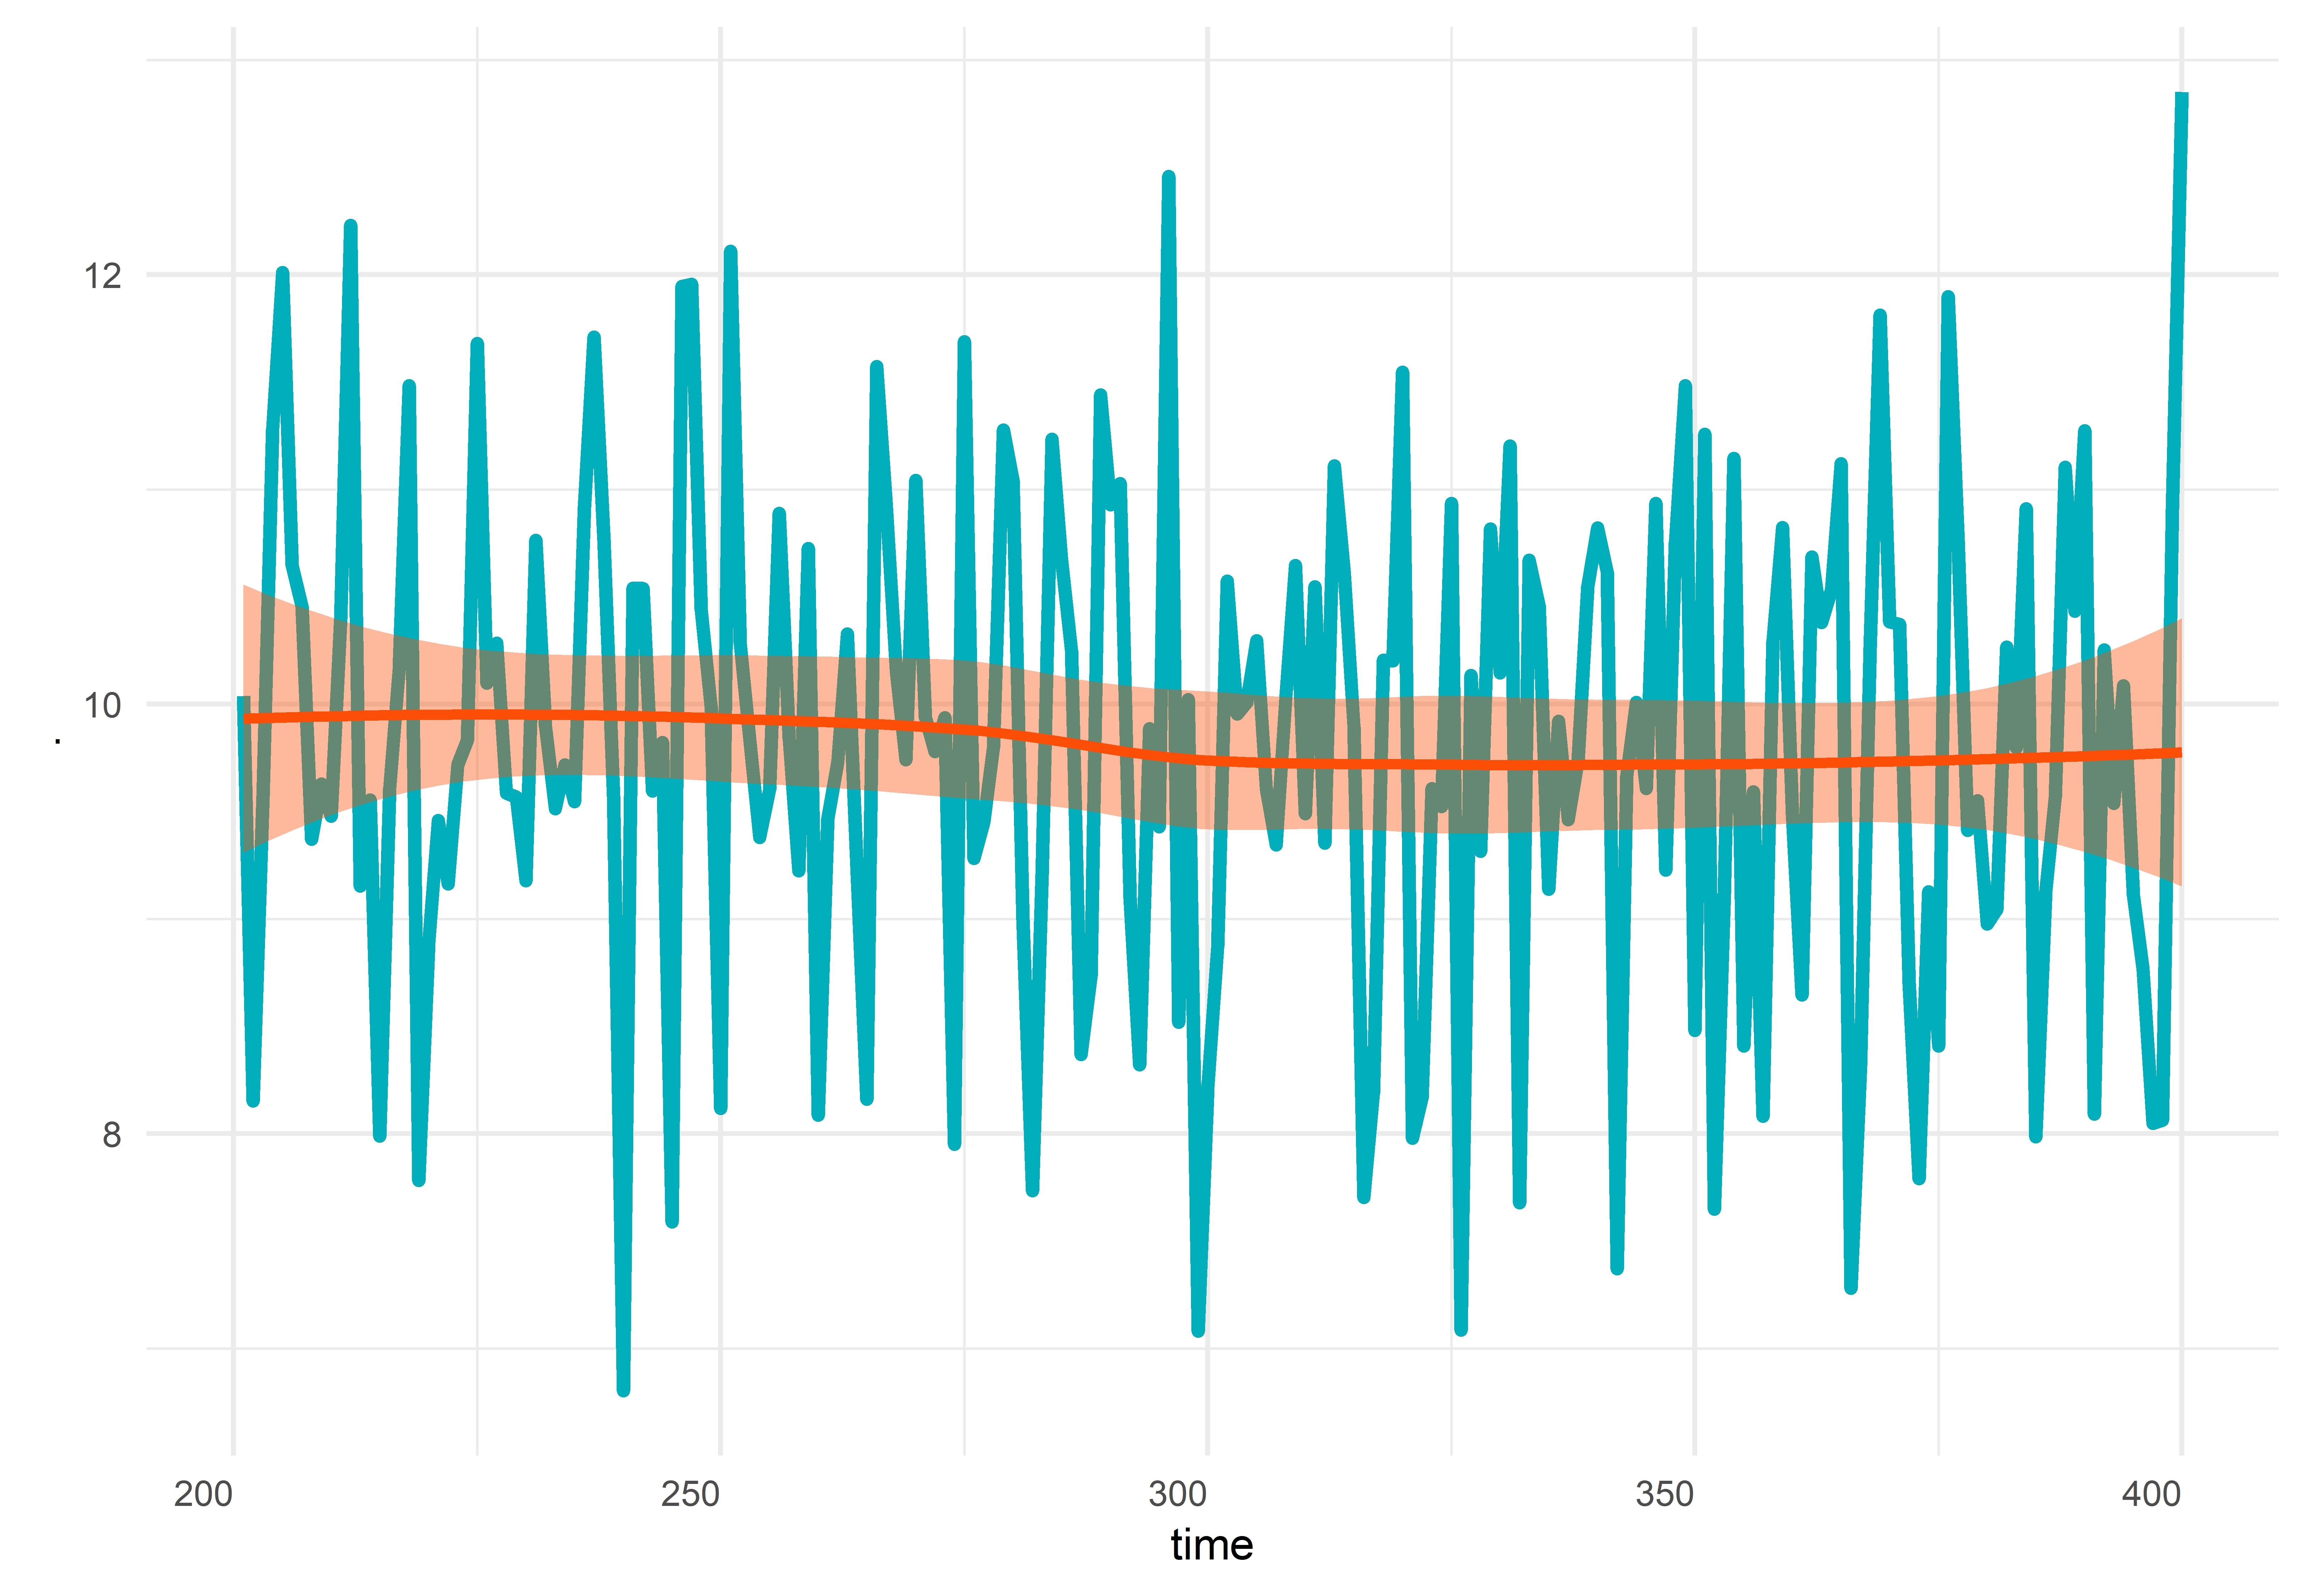
\includegraphics[width=1\linewidth,height=1\textheight]{Tesis_files/figure-latex/arima402_comportamiento-1} \caption{Tendencia de los datos simulados a partir de un proceso ARIMA(4,0,2)}\label{fig:arima402_comportamiento}
\end{figure}

\begin{figure}[H]
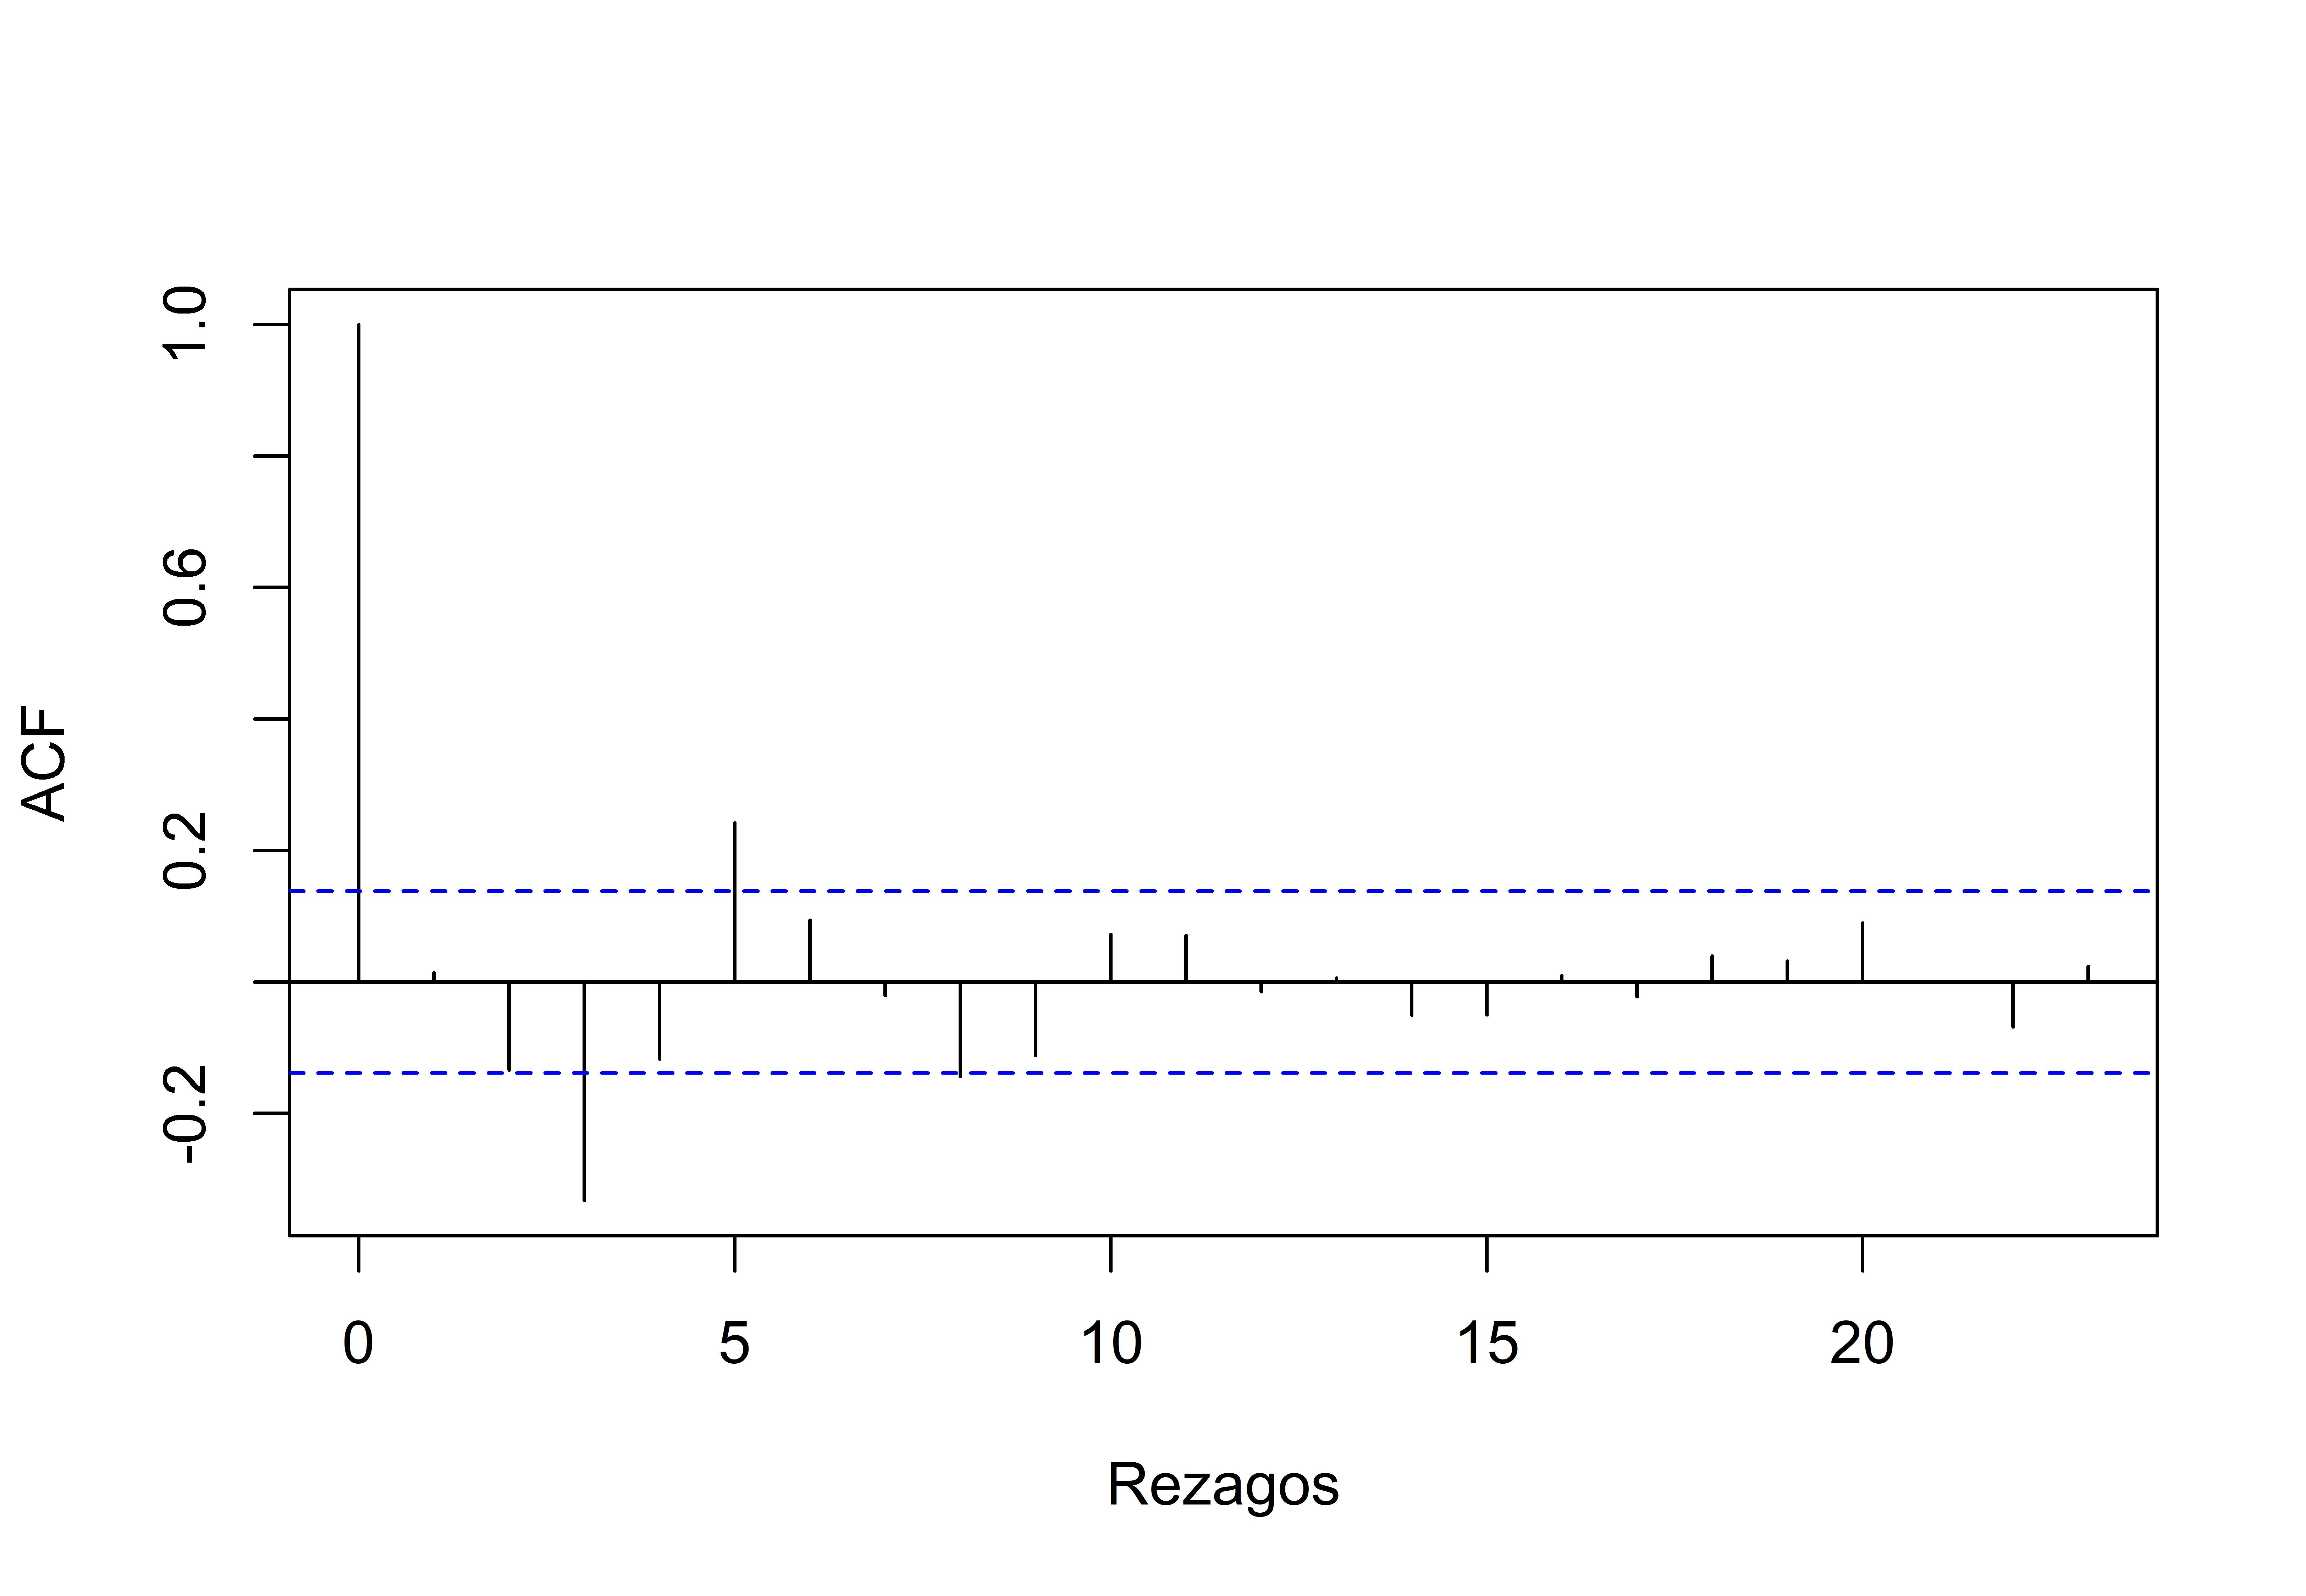
\includegraphics[width=1\linewidth,height=1\textheight]{Tesis_files/figure-latex/arima402_acf-1} \caption{Autocorrelación de los datos simulados a partir de un proceso ARIMA(4,0,2)}\label{fig:arima402_acf}
\end{figure}

\begin{figure}[H]
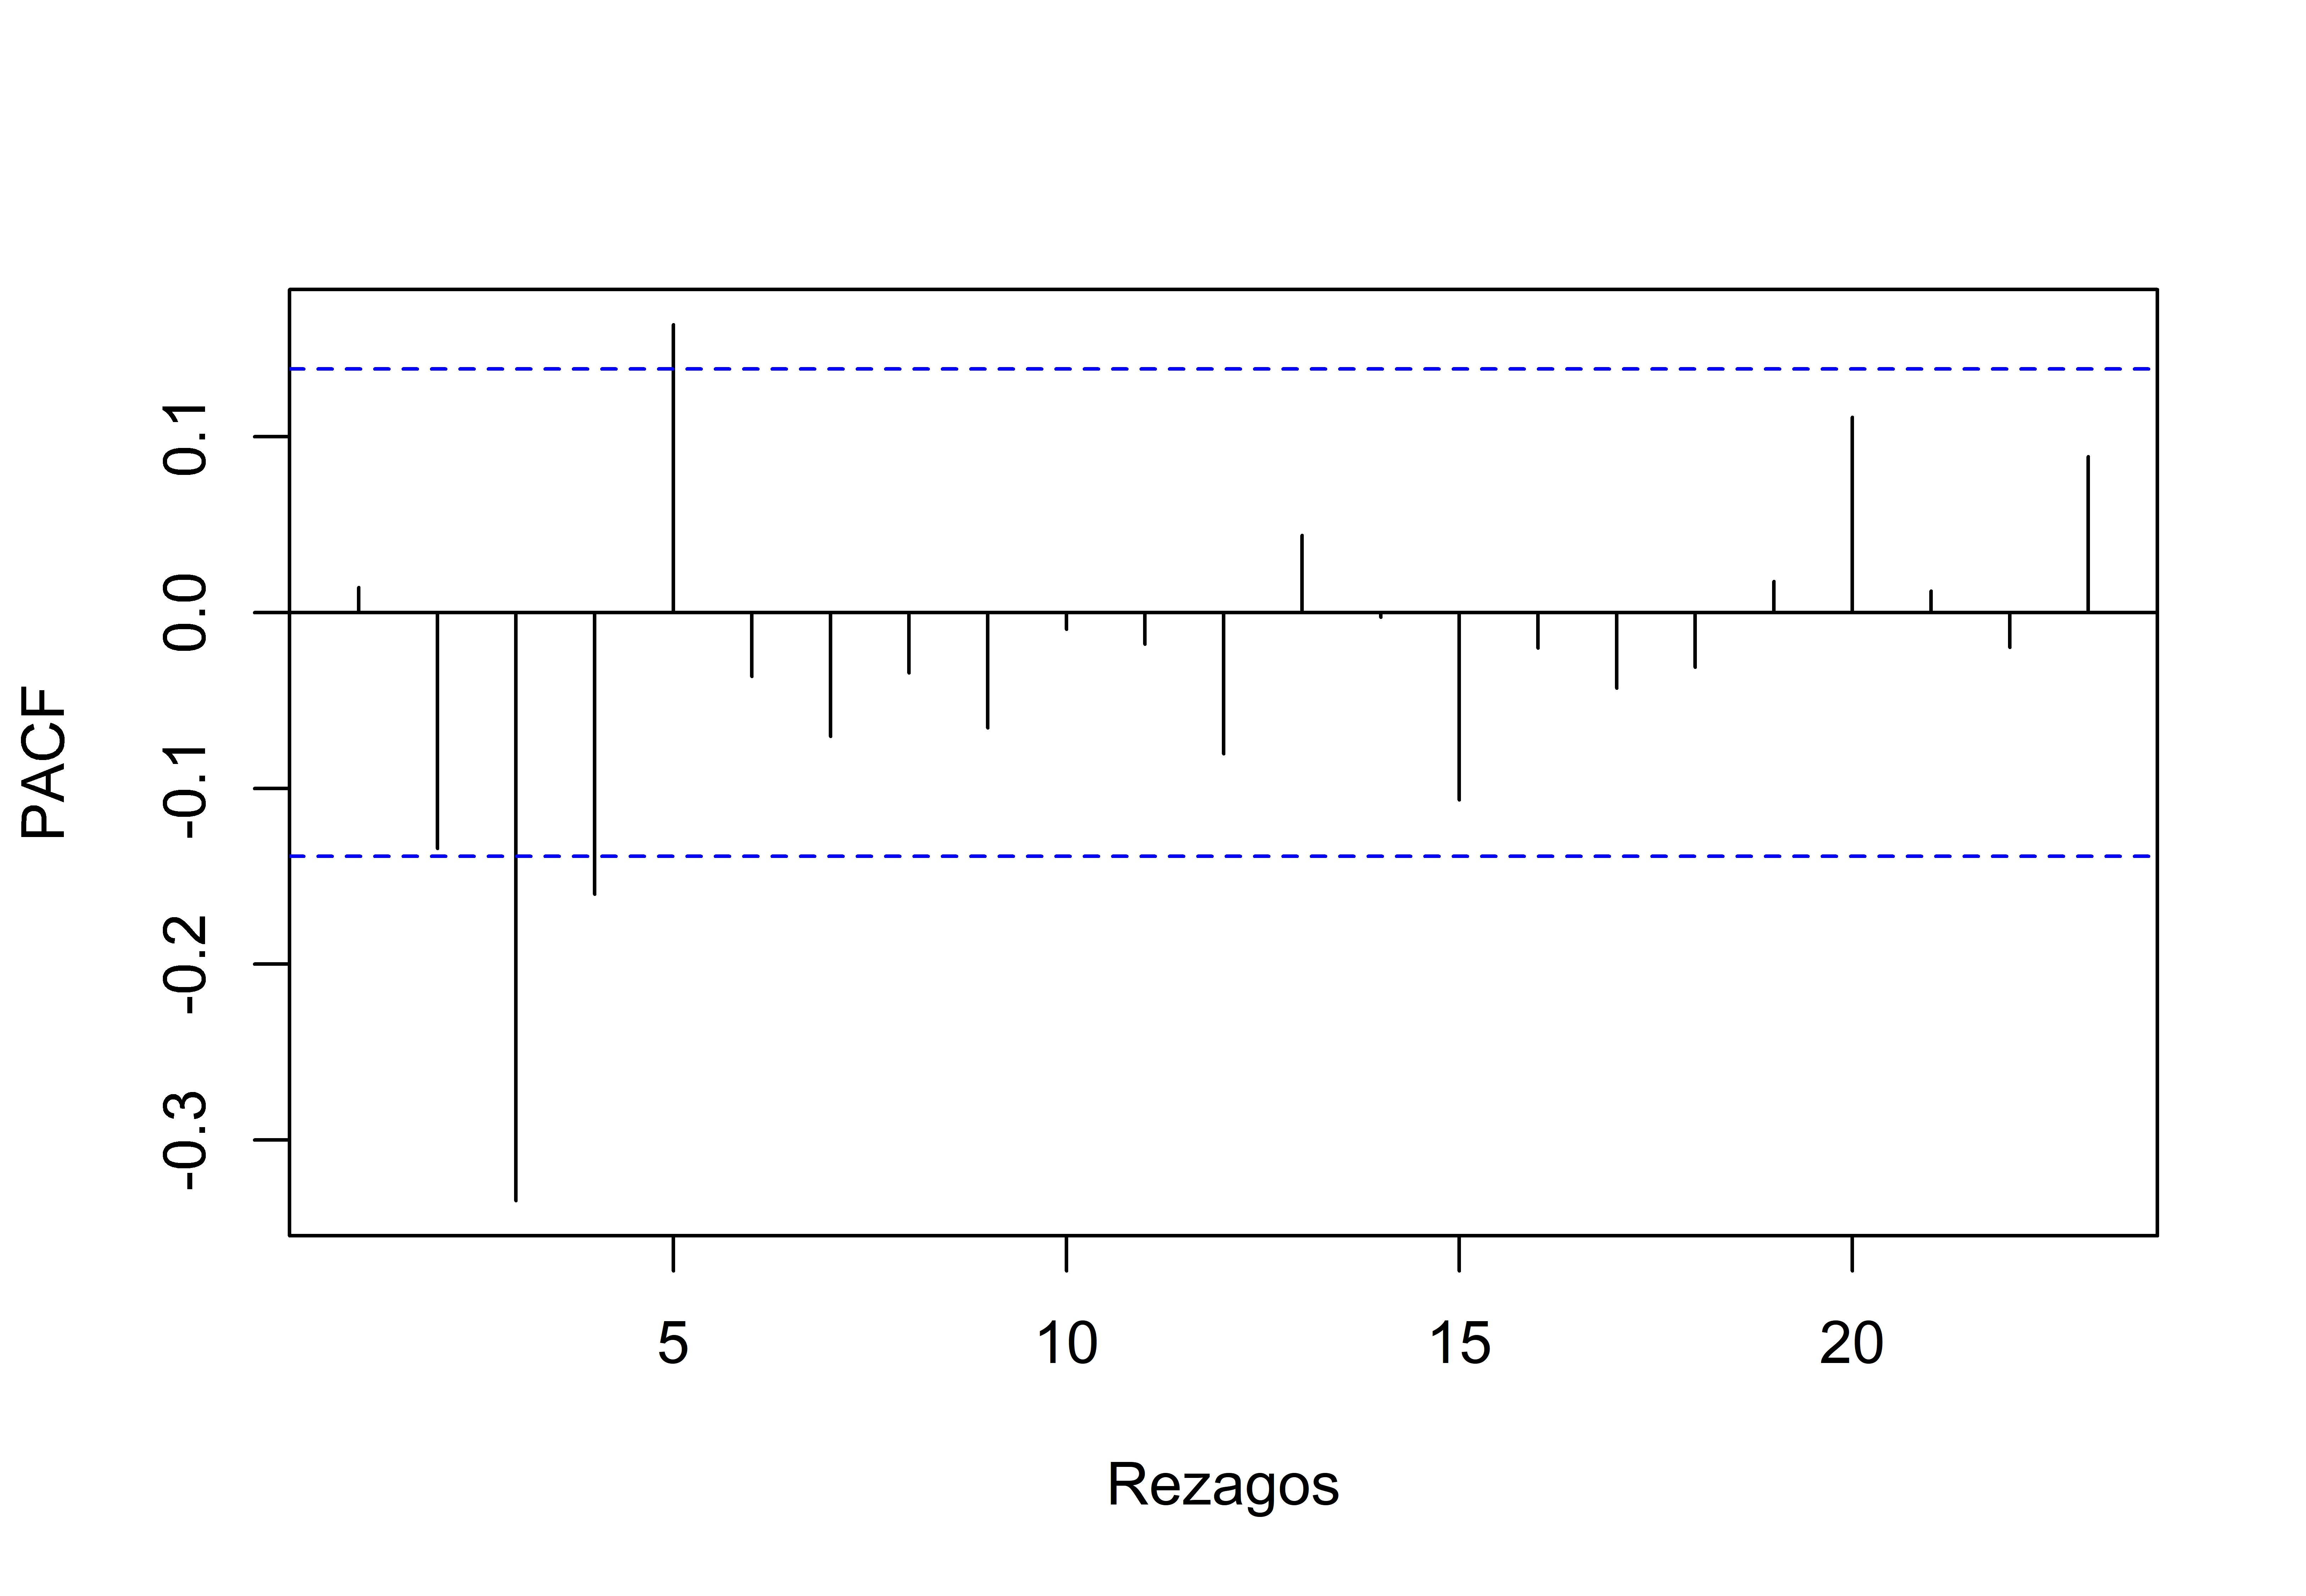
\includegraphics[width=1\linewidth,height=1\textheight]{Tesis_files/figure-latex/arima402_pacf-1} \caption{Autocorrelación parcial de los datos simulados a partir de un proceso ARIMA(4,0,2)}\label{fig:arima402_pacf}
\end{figure}

\paragraph{ARIMA(0,0,1)(0,1,1)}

En la figura \ref{fig:arima001_011_comportamiento} los datos parecen ser
aproximadamente estacionarios, pero esto no es del todo claro; una
transformación no es estrictamente necesaria, pero puede aplicarse para
corregir ligeramente la parte estacional. Las figuras
\ref{fig:arima001_011_acf} y \ref{fig:arima001_011_pacf}, sugieren estar
en presencia de un proceso estacional cada 12 periodos, por lo que la
estimación de modelos \(ARIMA\) de bajo nivel podría ser suficiente..

\begin{figure}[H]
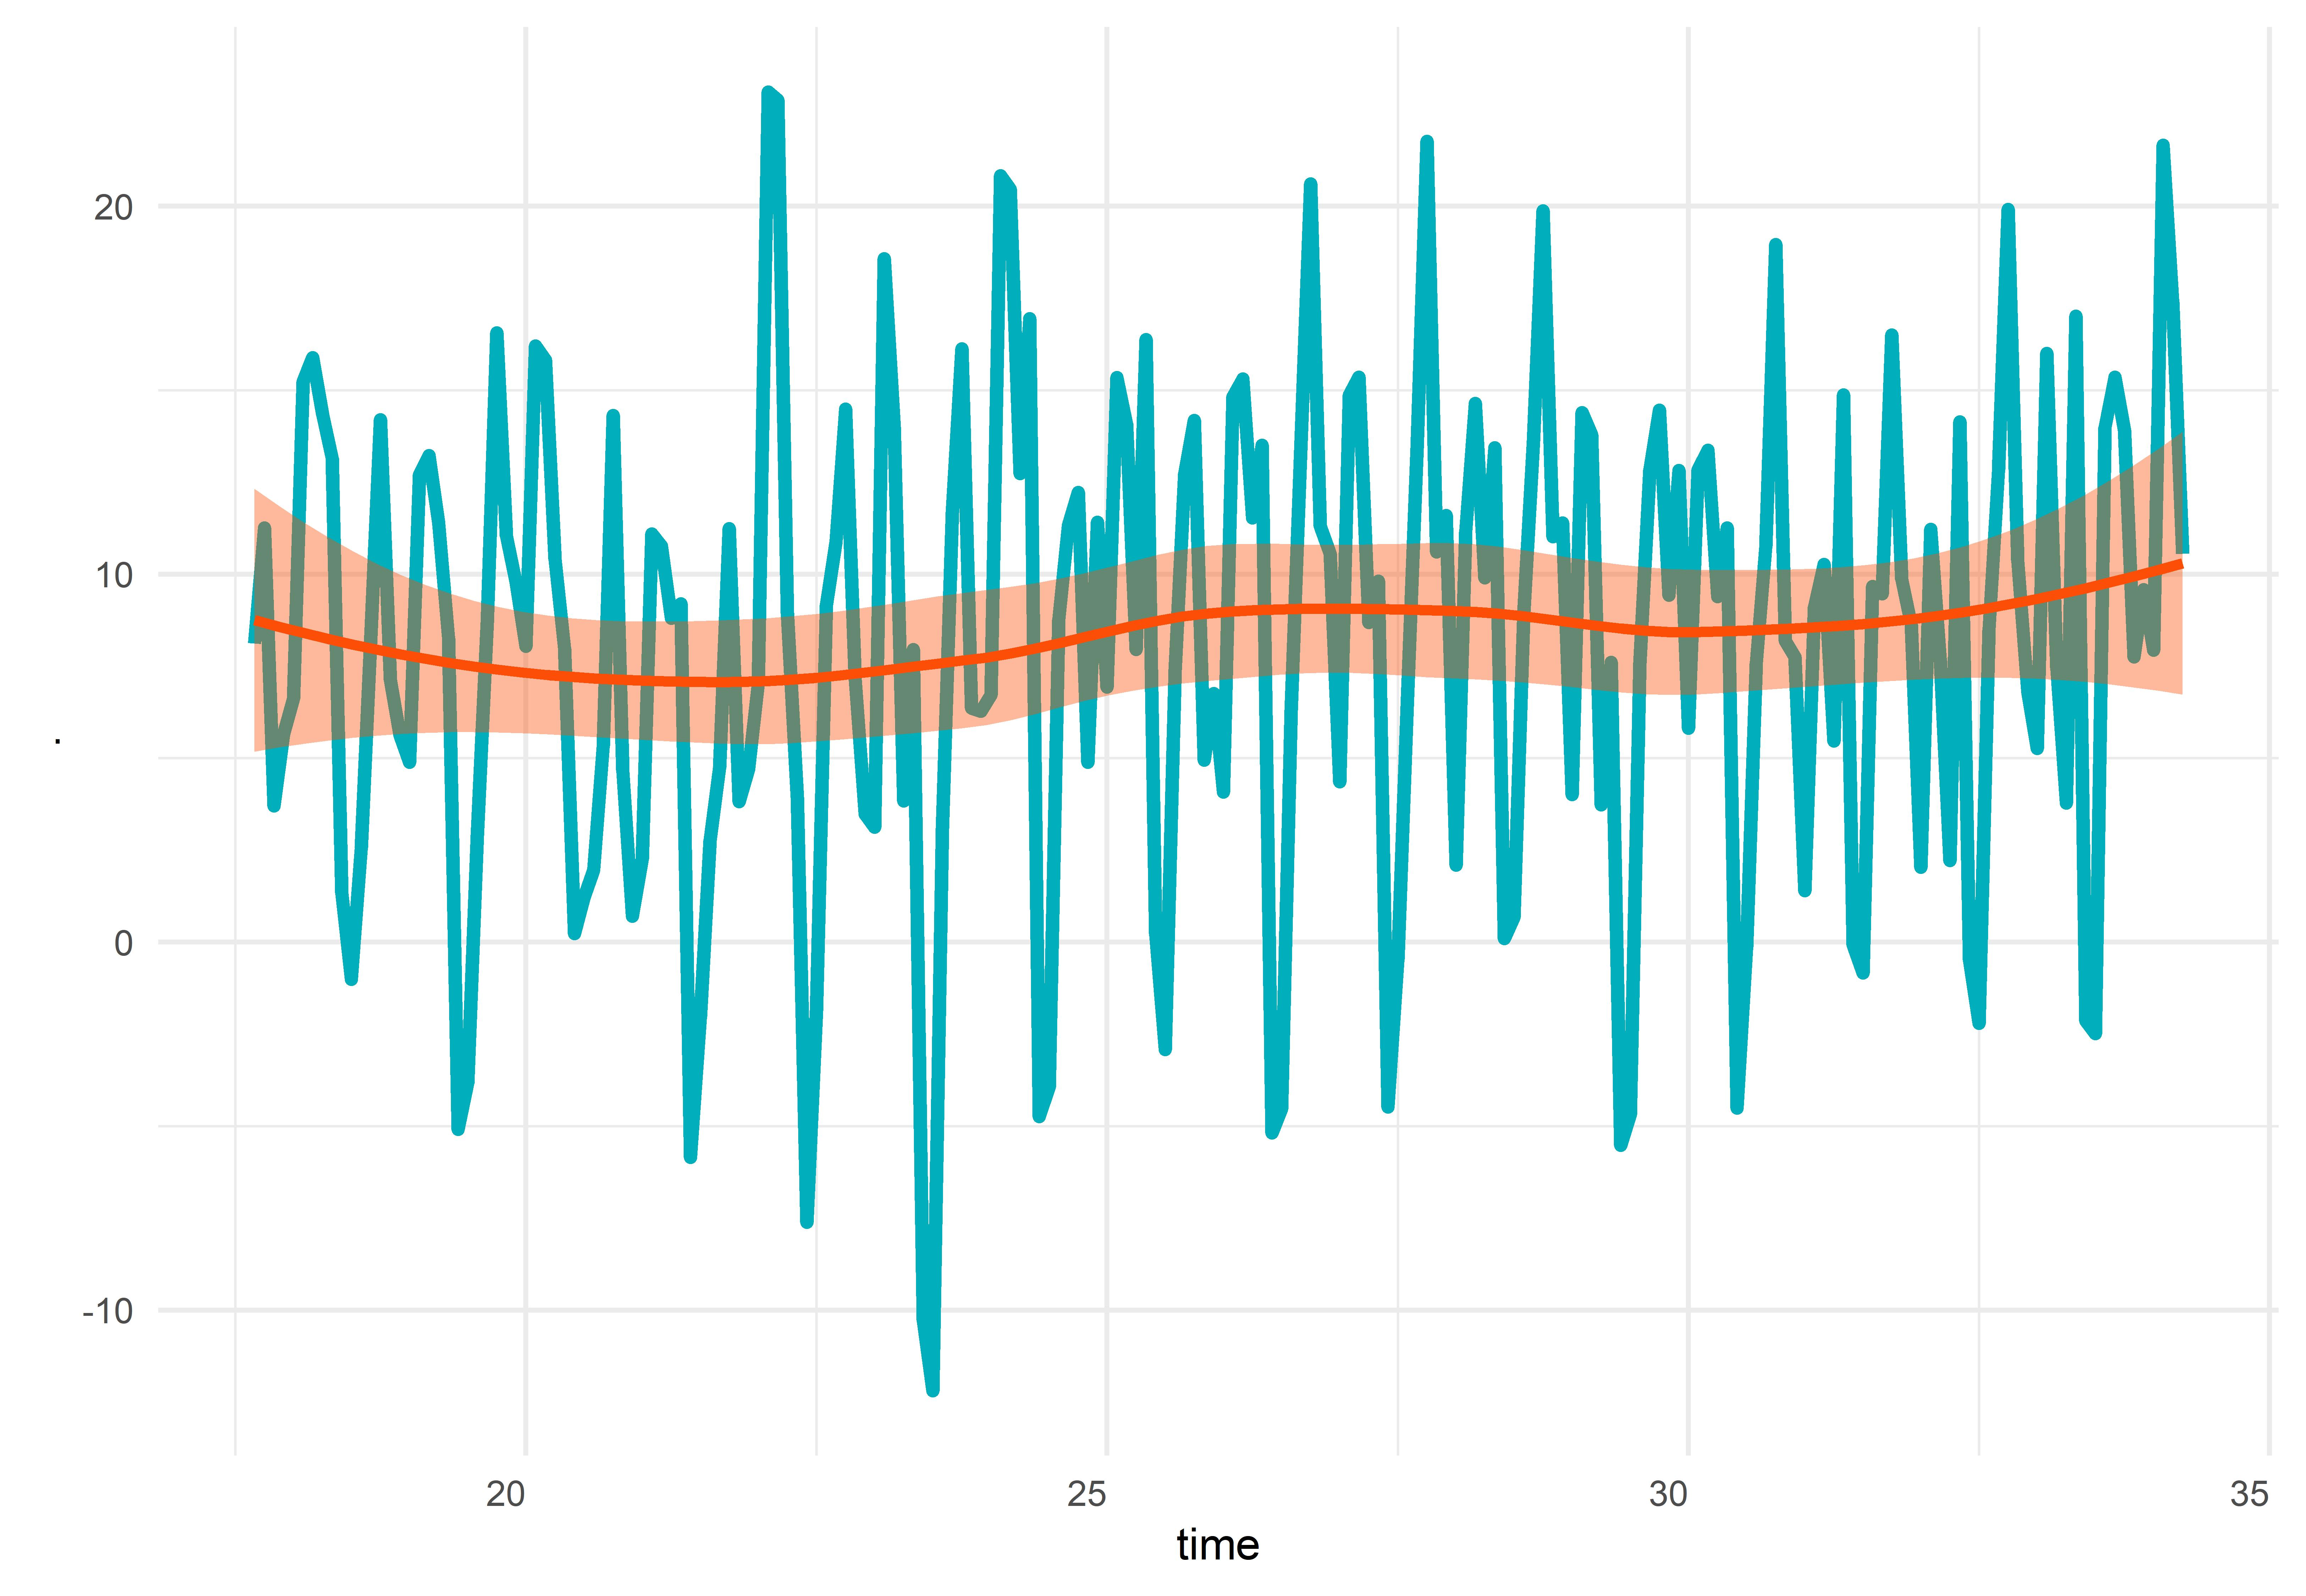
\includegraphics[width=1\linewidth,height=1\textheight]{Tesis_files/figure-latex/arima001_011_comportamiento-1} \caption{Tendencia de los datos simulados a partir de un proceso ARIMA(0,0,1)(0,1,1)}\label{fig:arima001_011_comportamiento}
\end{figure}

\begin{figure}[H]
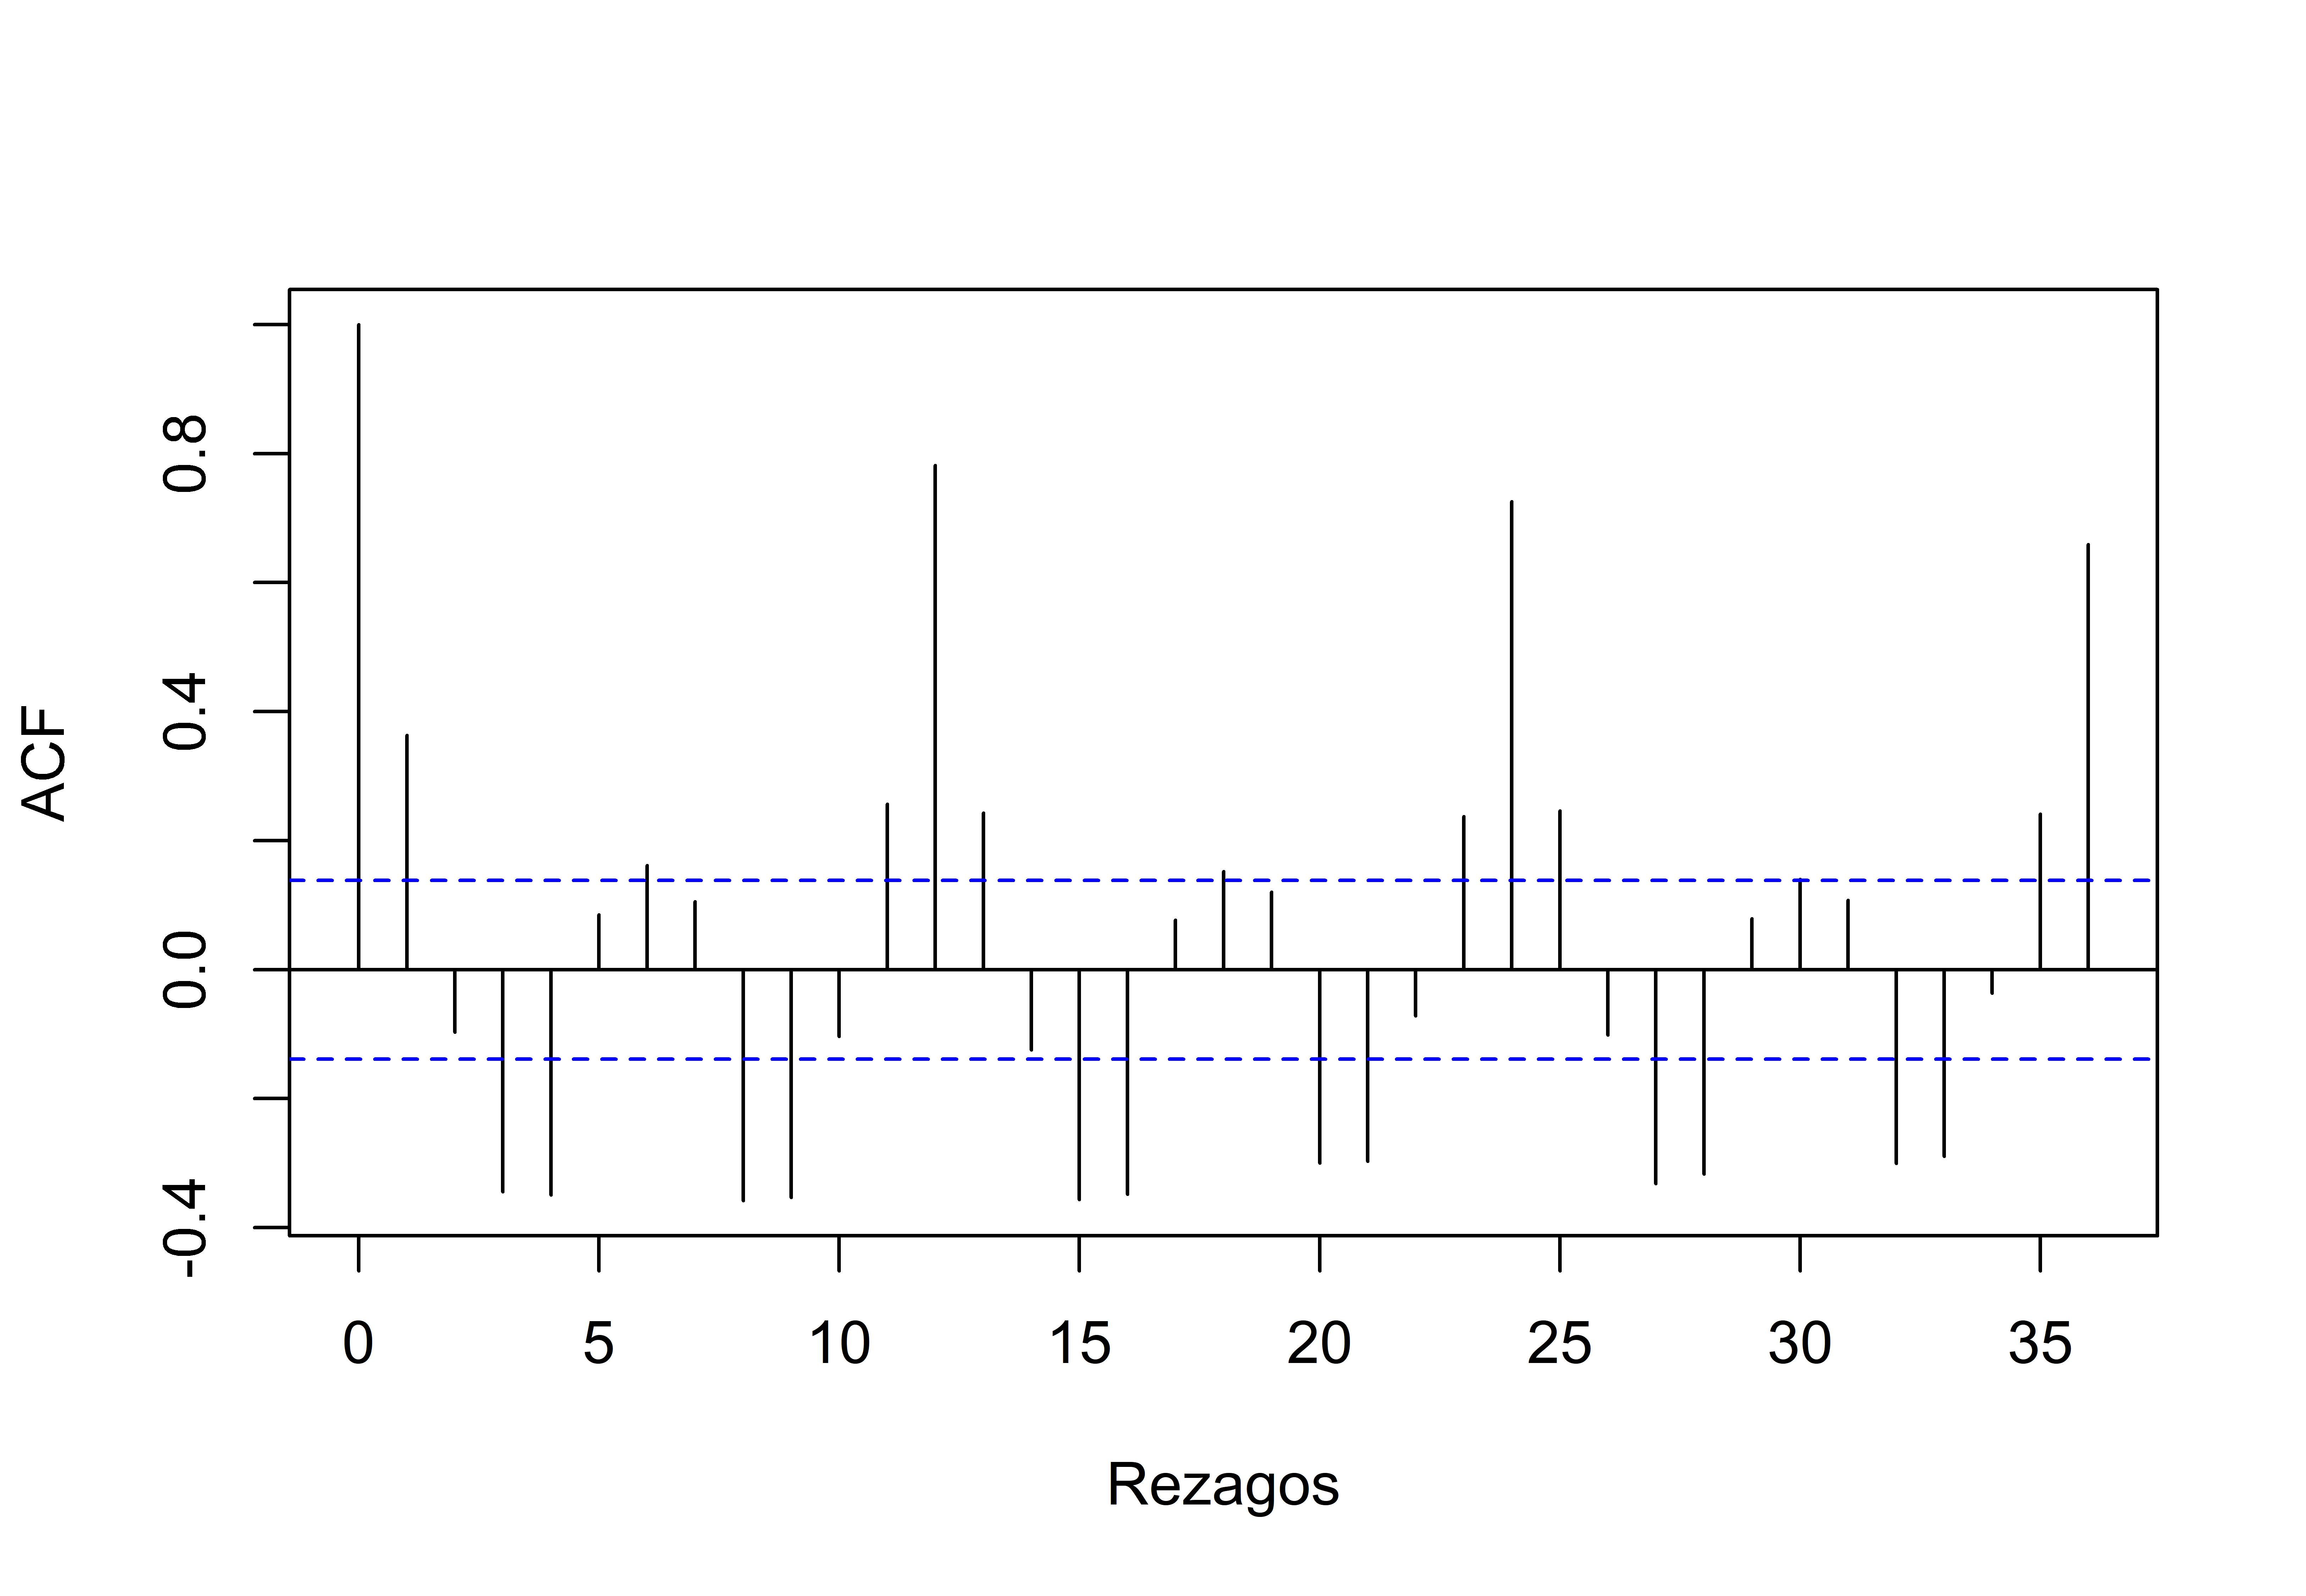
\includegraphics[width=1\linewidth,height=1\textheight]{Tesis_files/figure-latex/arima001_011_acf-1} \caption{Autocorrelación de los datos simulados a partir de un proceso ARIMA(0,0,1)(0,1,1)}\label{fig:arima001_011_acf}
\end{figure}

\begin{figure}[H]
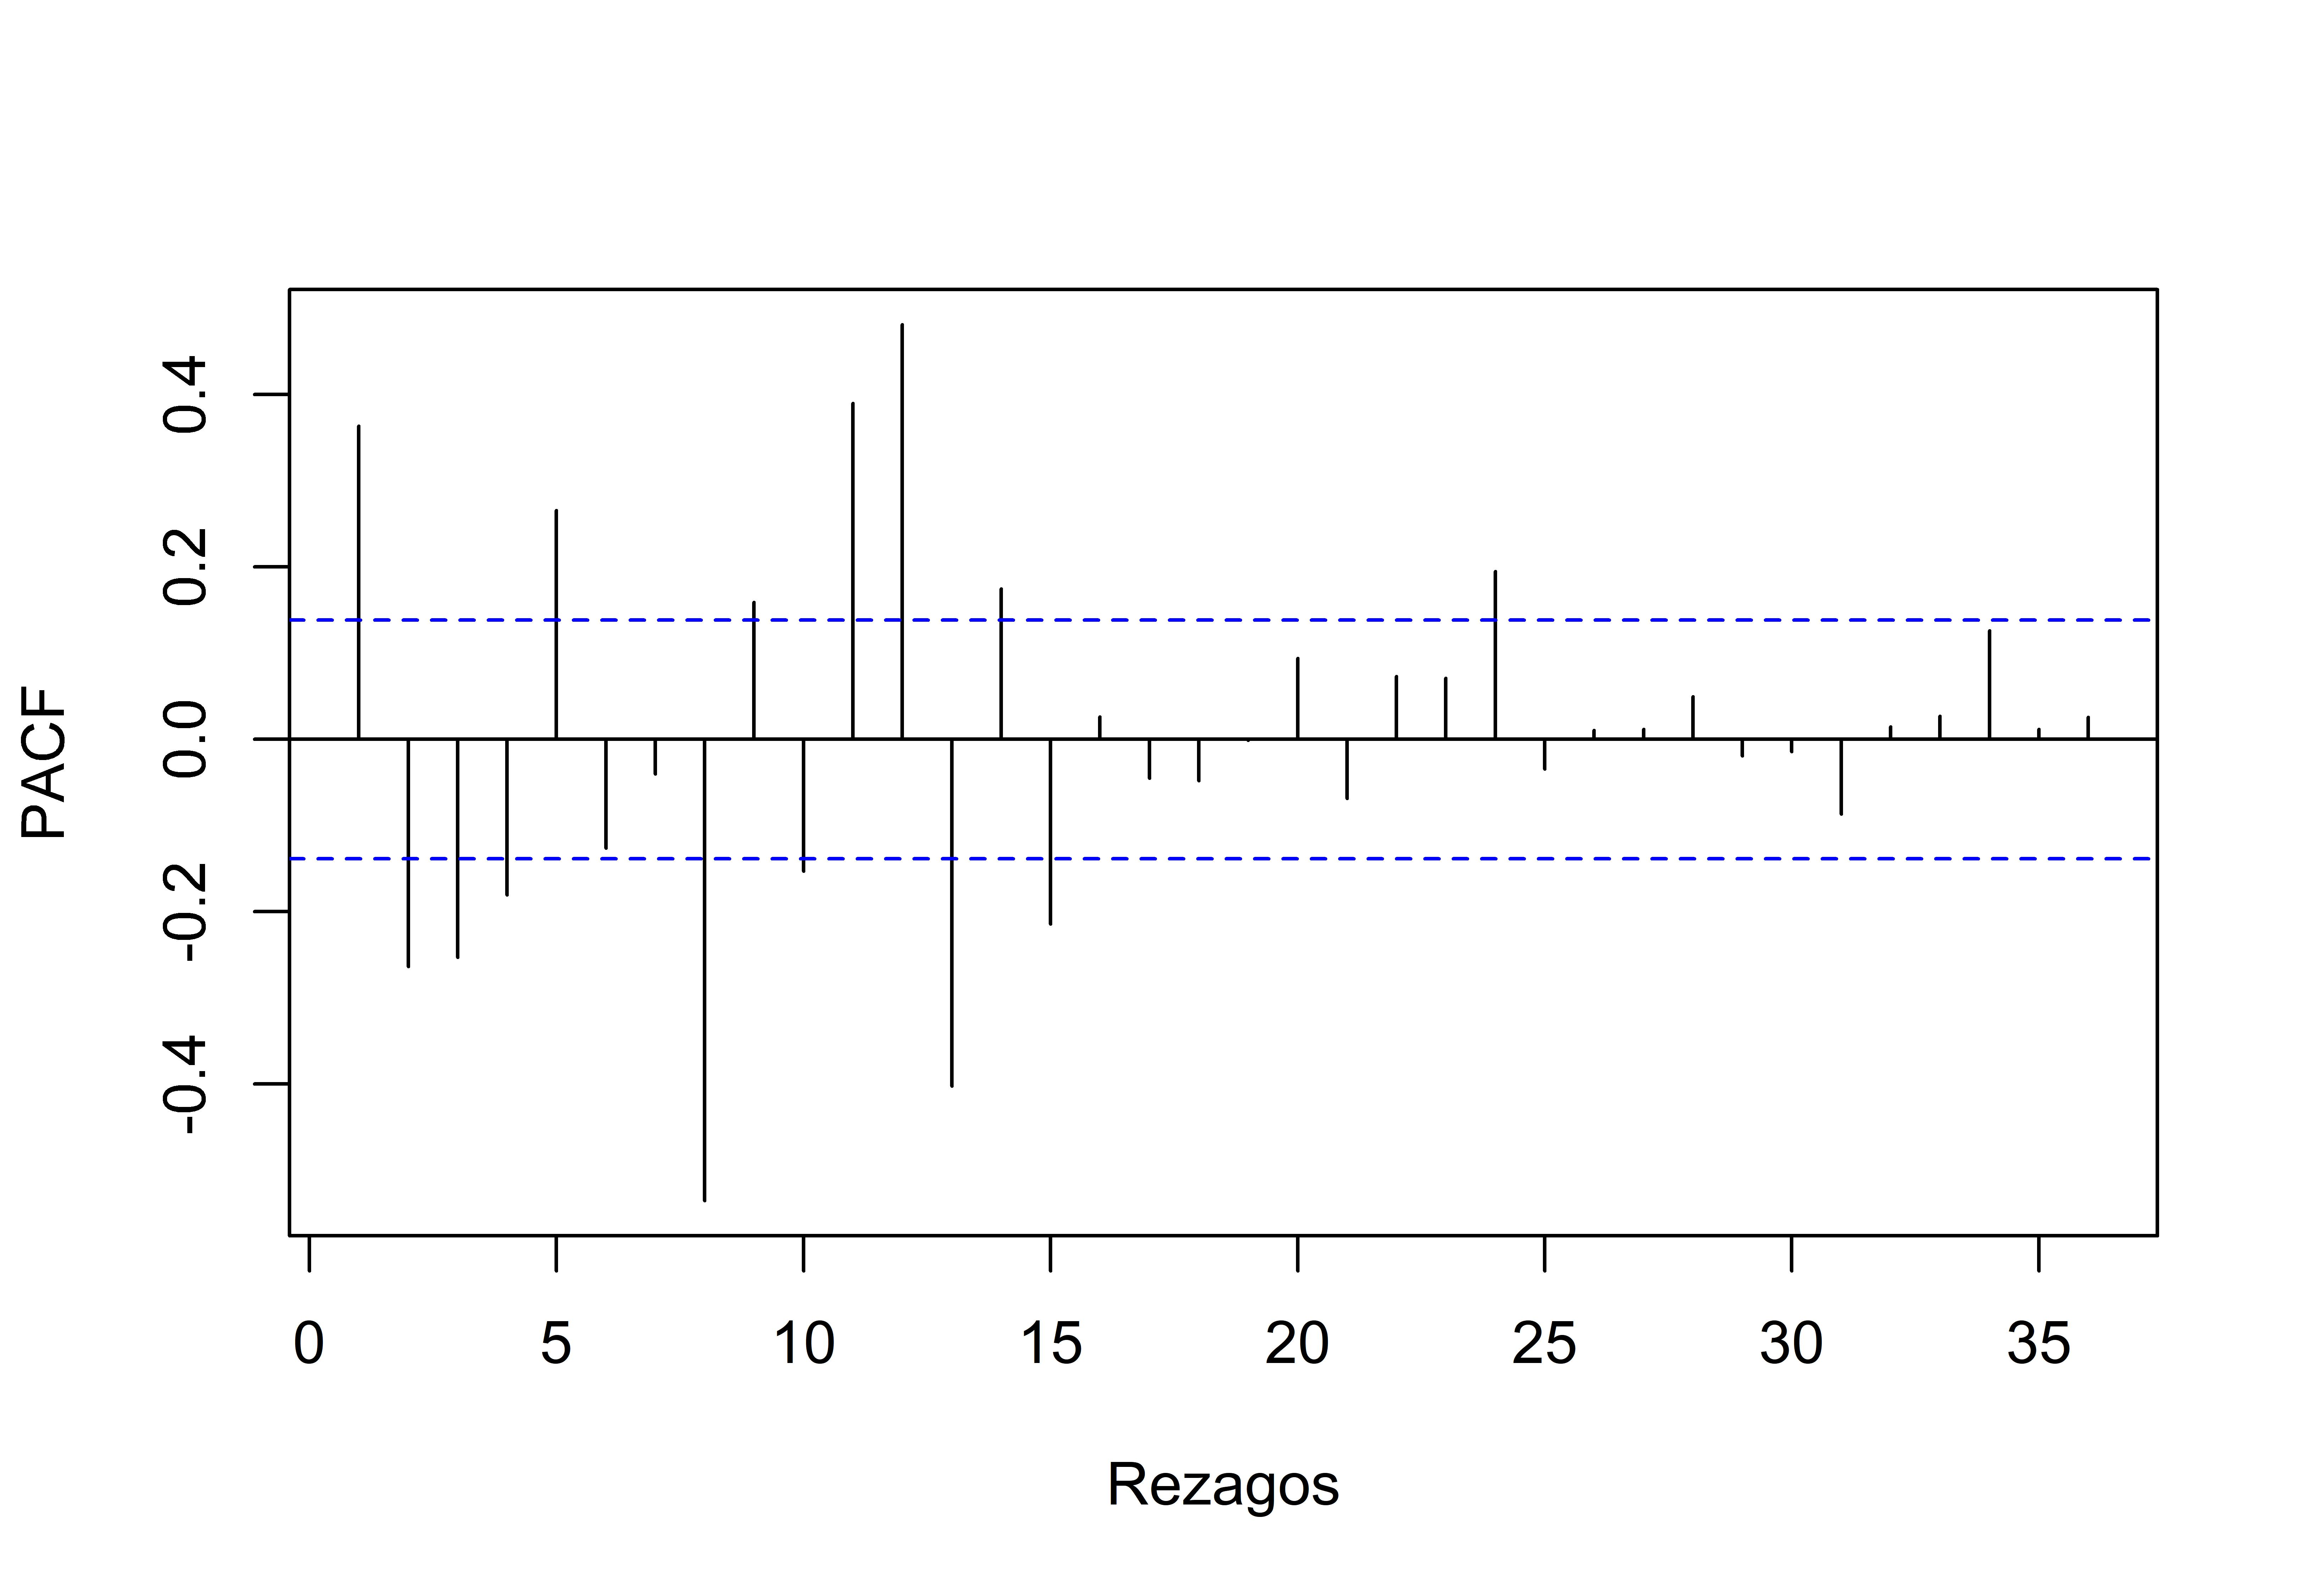
\includegraphics[width=1\linewidth,height=1\textheight]{Tesis_files/figure-latex/arima001_011_pacf-1} \caption{Autocorrelación parcial de los datos simulados a partir de un proceso ARIMA(0,0,1)(0,1,1)}\label{fig:arima001_011_pacf}
\end{figure}

\paragraph{ARIMA(2,1,4)(3,0,3)}

En la figura \ref{fig:arima214_303_comportamiento} se manifiesta una
clara tendencia bajista. Las figuras \ref{fig:arima214_303_acf} y
\ref{fig:arima214_303_pacf} no permiten identificar claramente el
proceso que gobierna la serie, por lo que habría que probar distintos
modelos \(ARIMA\) hasta encontrar el más adecuado.

\begin{figure}[H]
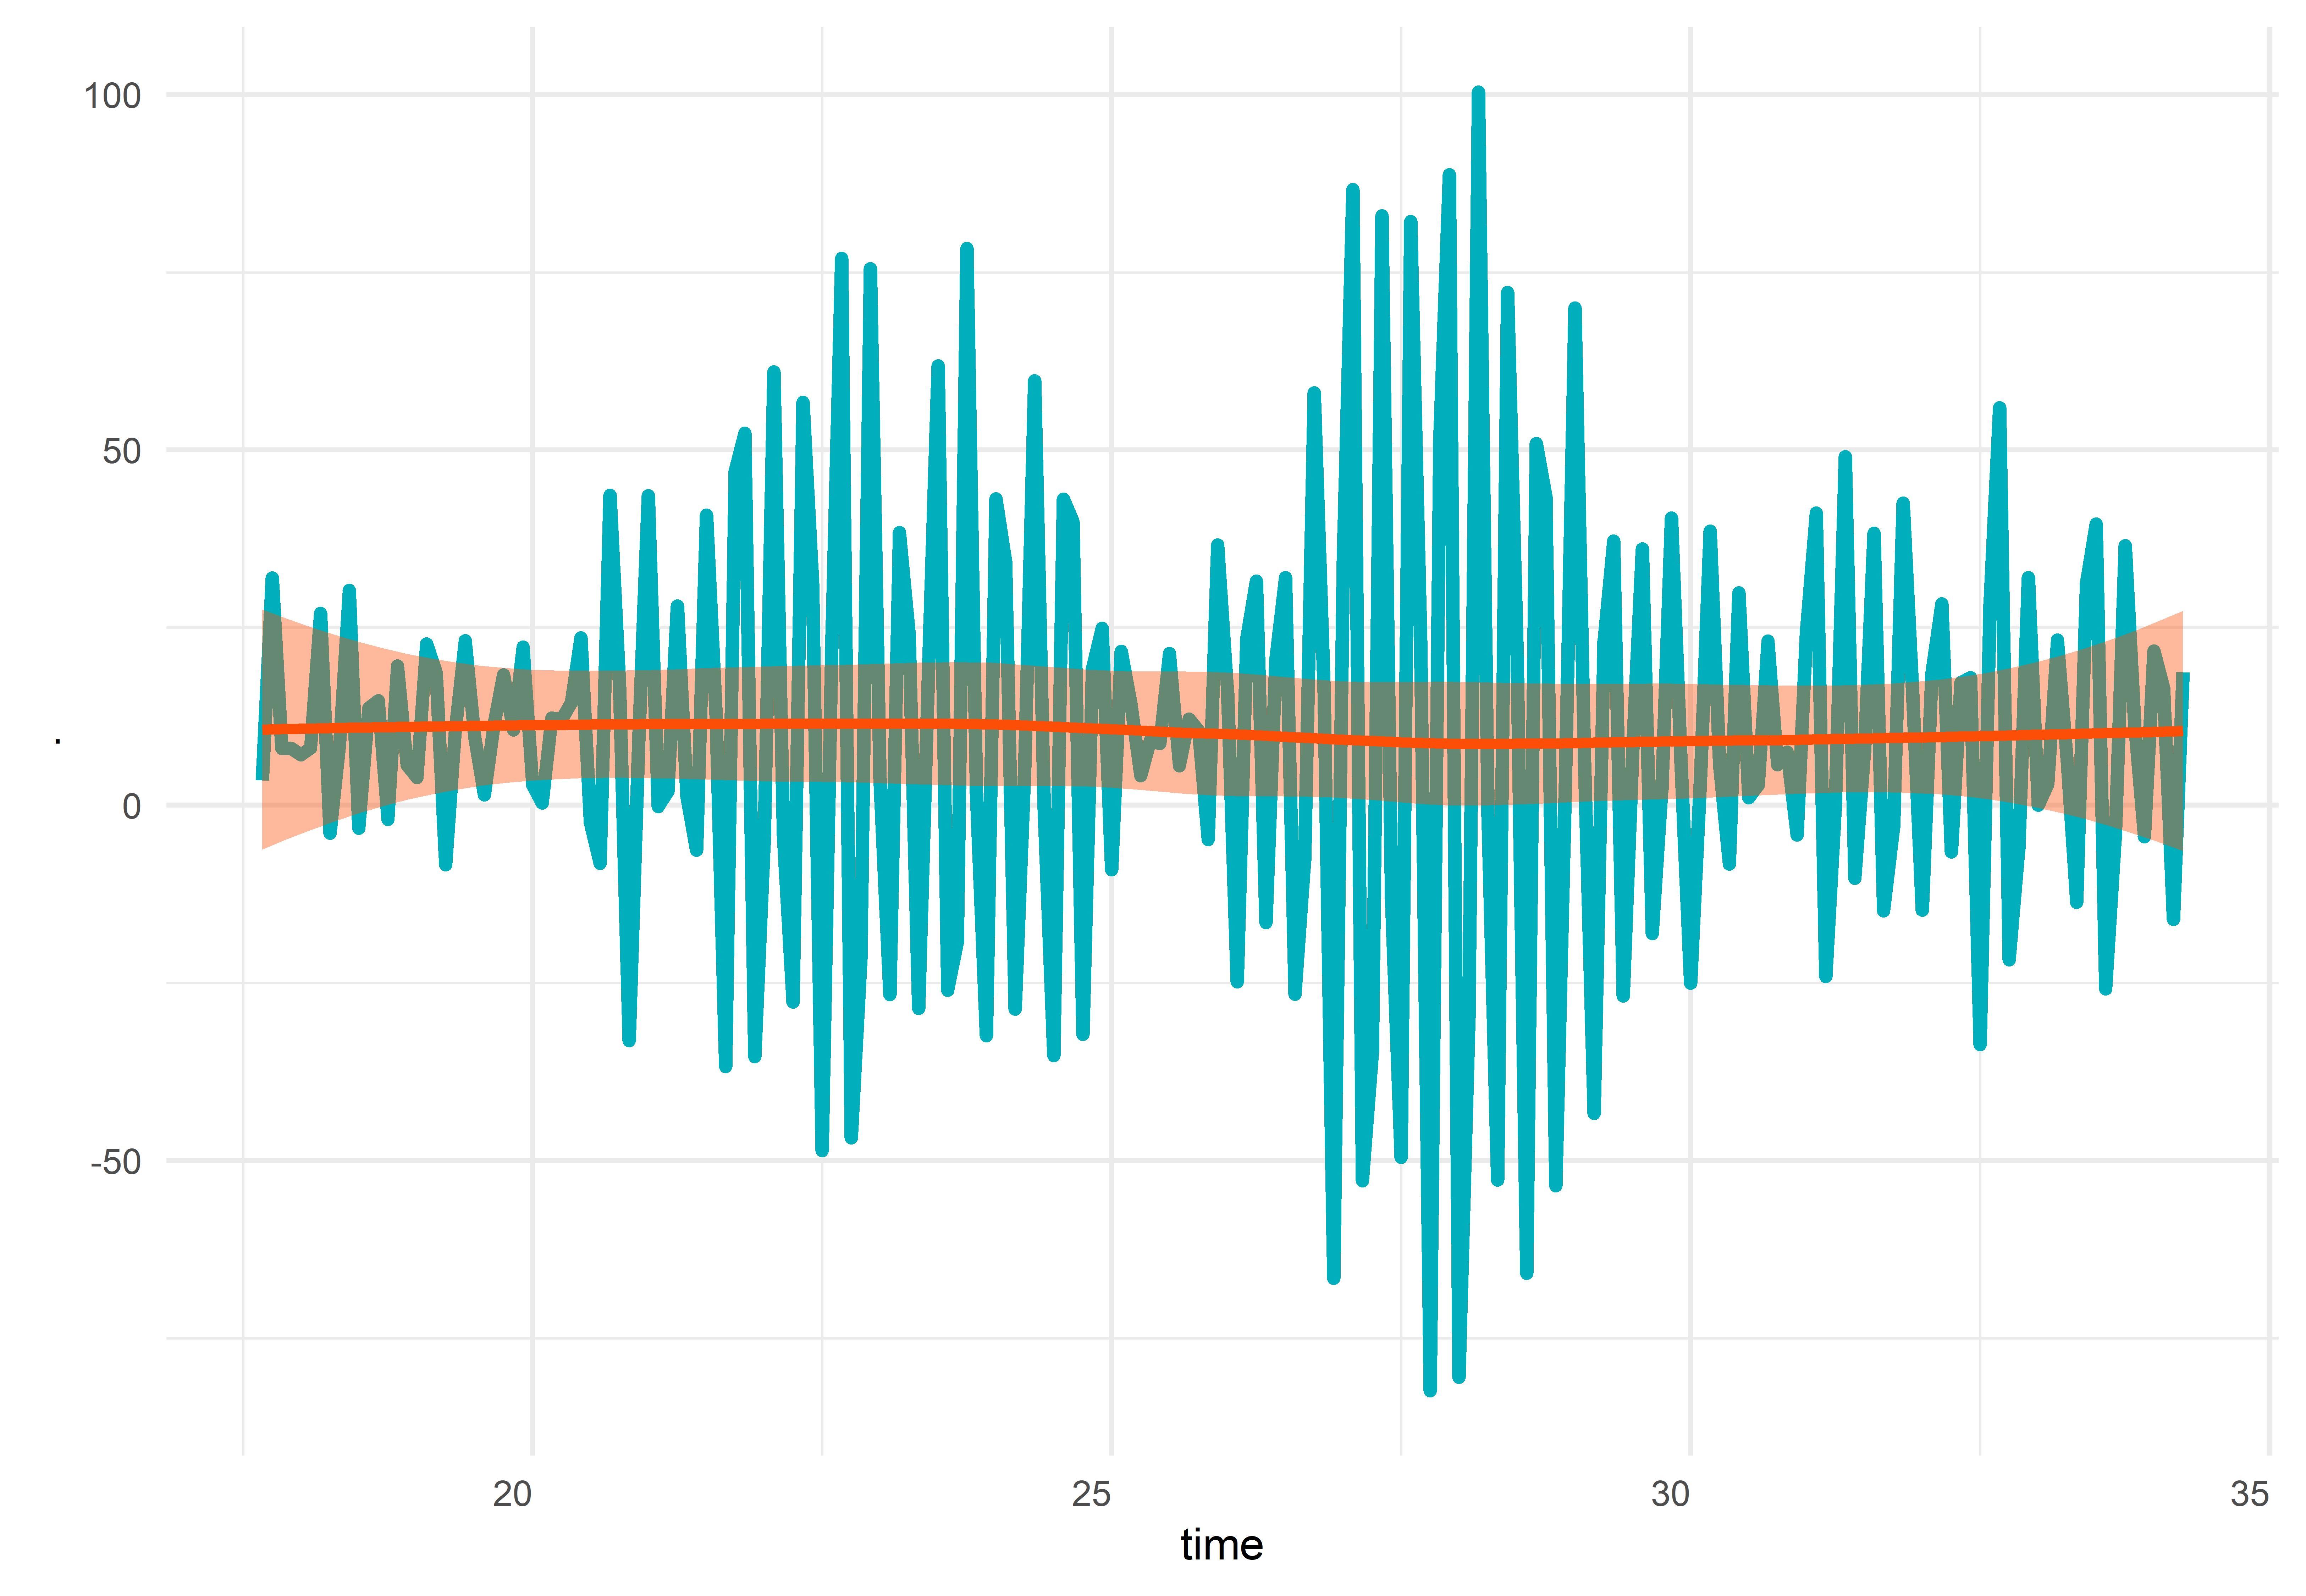
\includegraphics[width=1\linewidth,height=1\textheight]{Tesis_files/figure-latex/arima214_303_comportamiento-1} \caption{Tendencia de los datos simulados a partir de un proceso ARIMA(2,1,4)(3,0,3)}\label{fig:arima214_303_comportamiento}
\end{figure}

\begin{figure}[H]
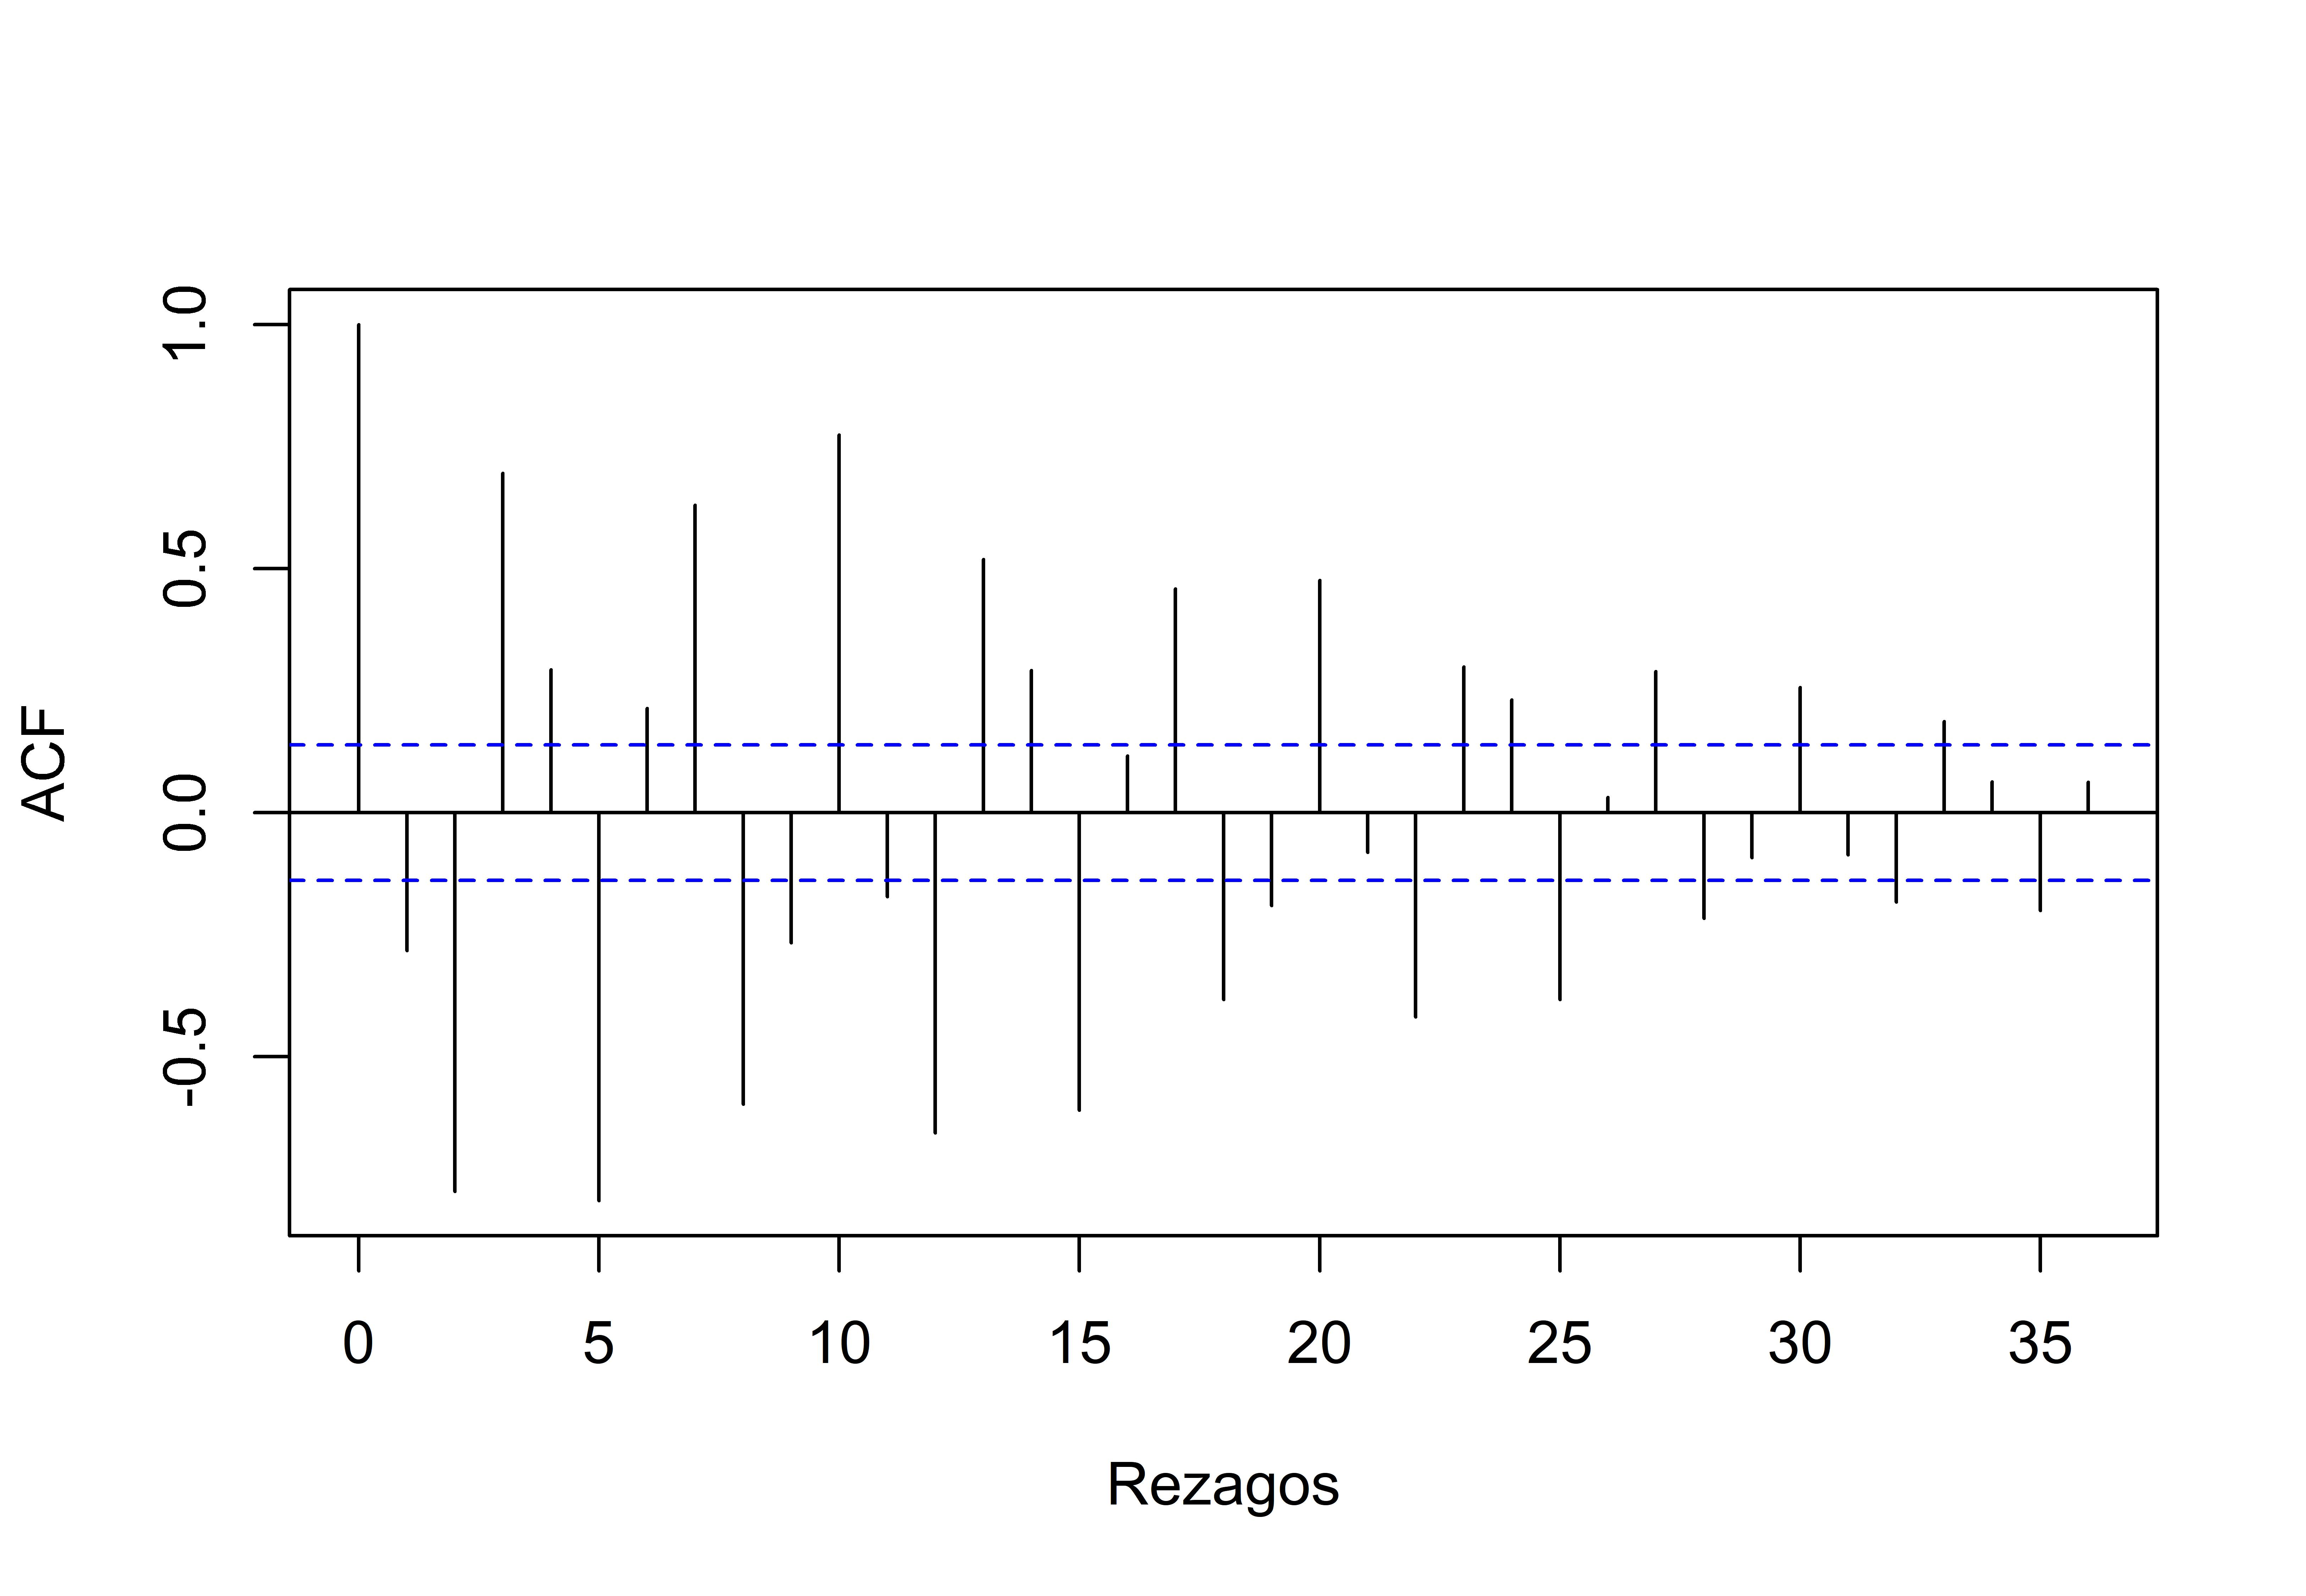
\includegraphics[width=1\linewidth,height=1\textheight]{Tesis_files/figure-latex/arima214_303_acf-1} \caption{Autocorrelación de los datos simulados a partir de un proceso ARIMA(2,1,4)(3,0,3)}\label{fig:arima214_303_acf}
\end{figure}

\begin{figure}[H]
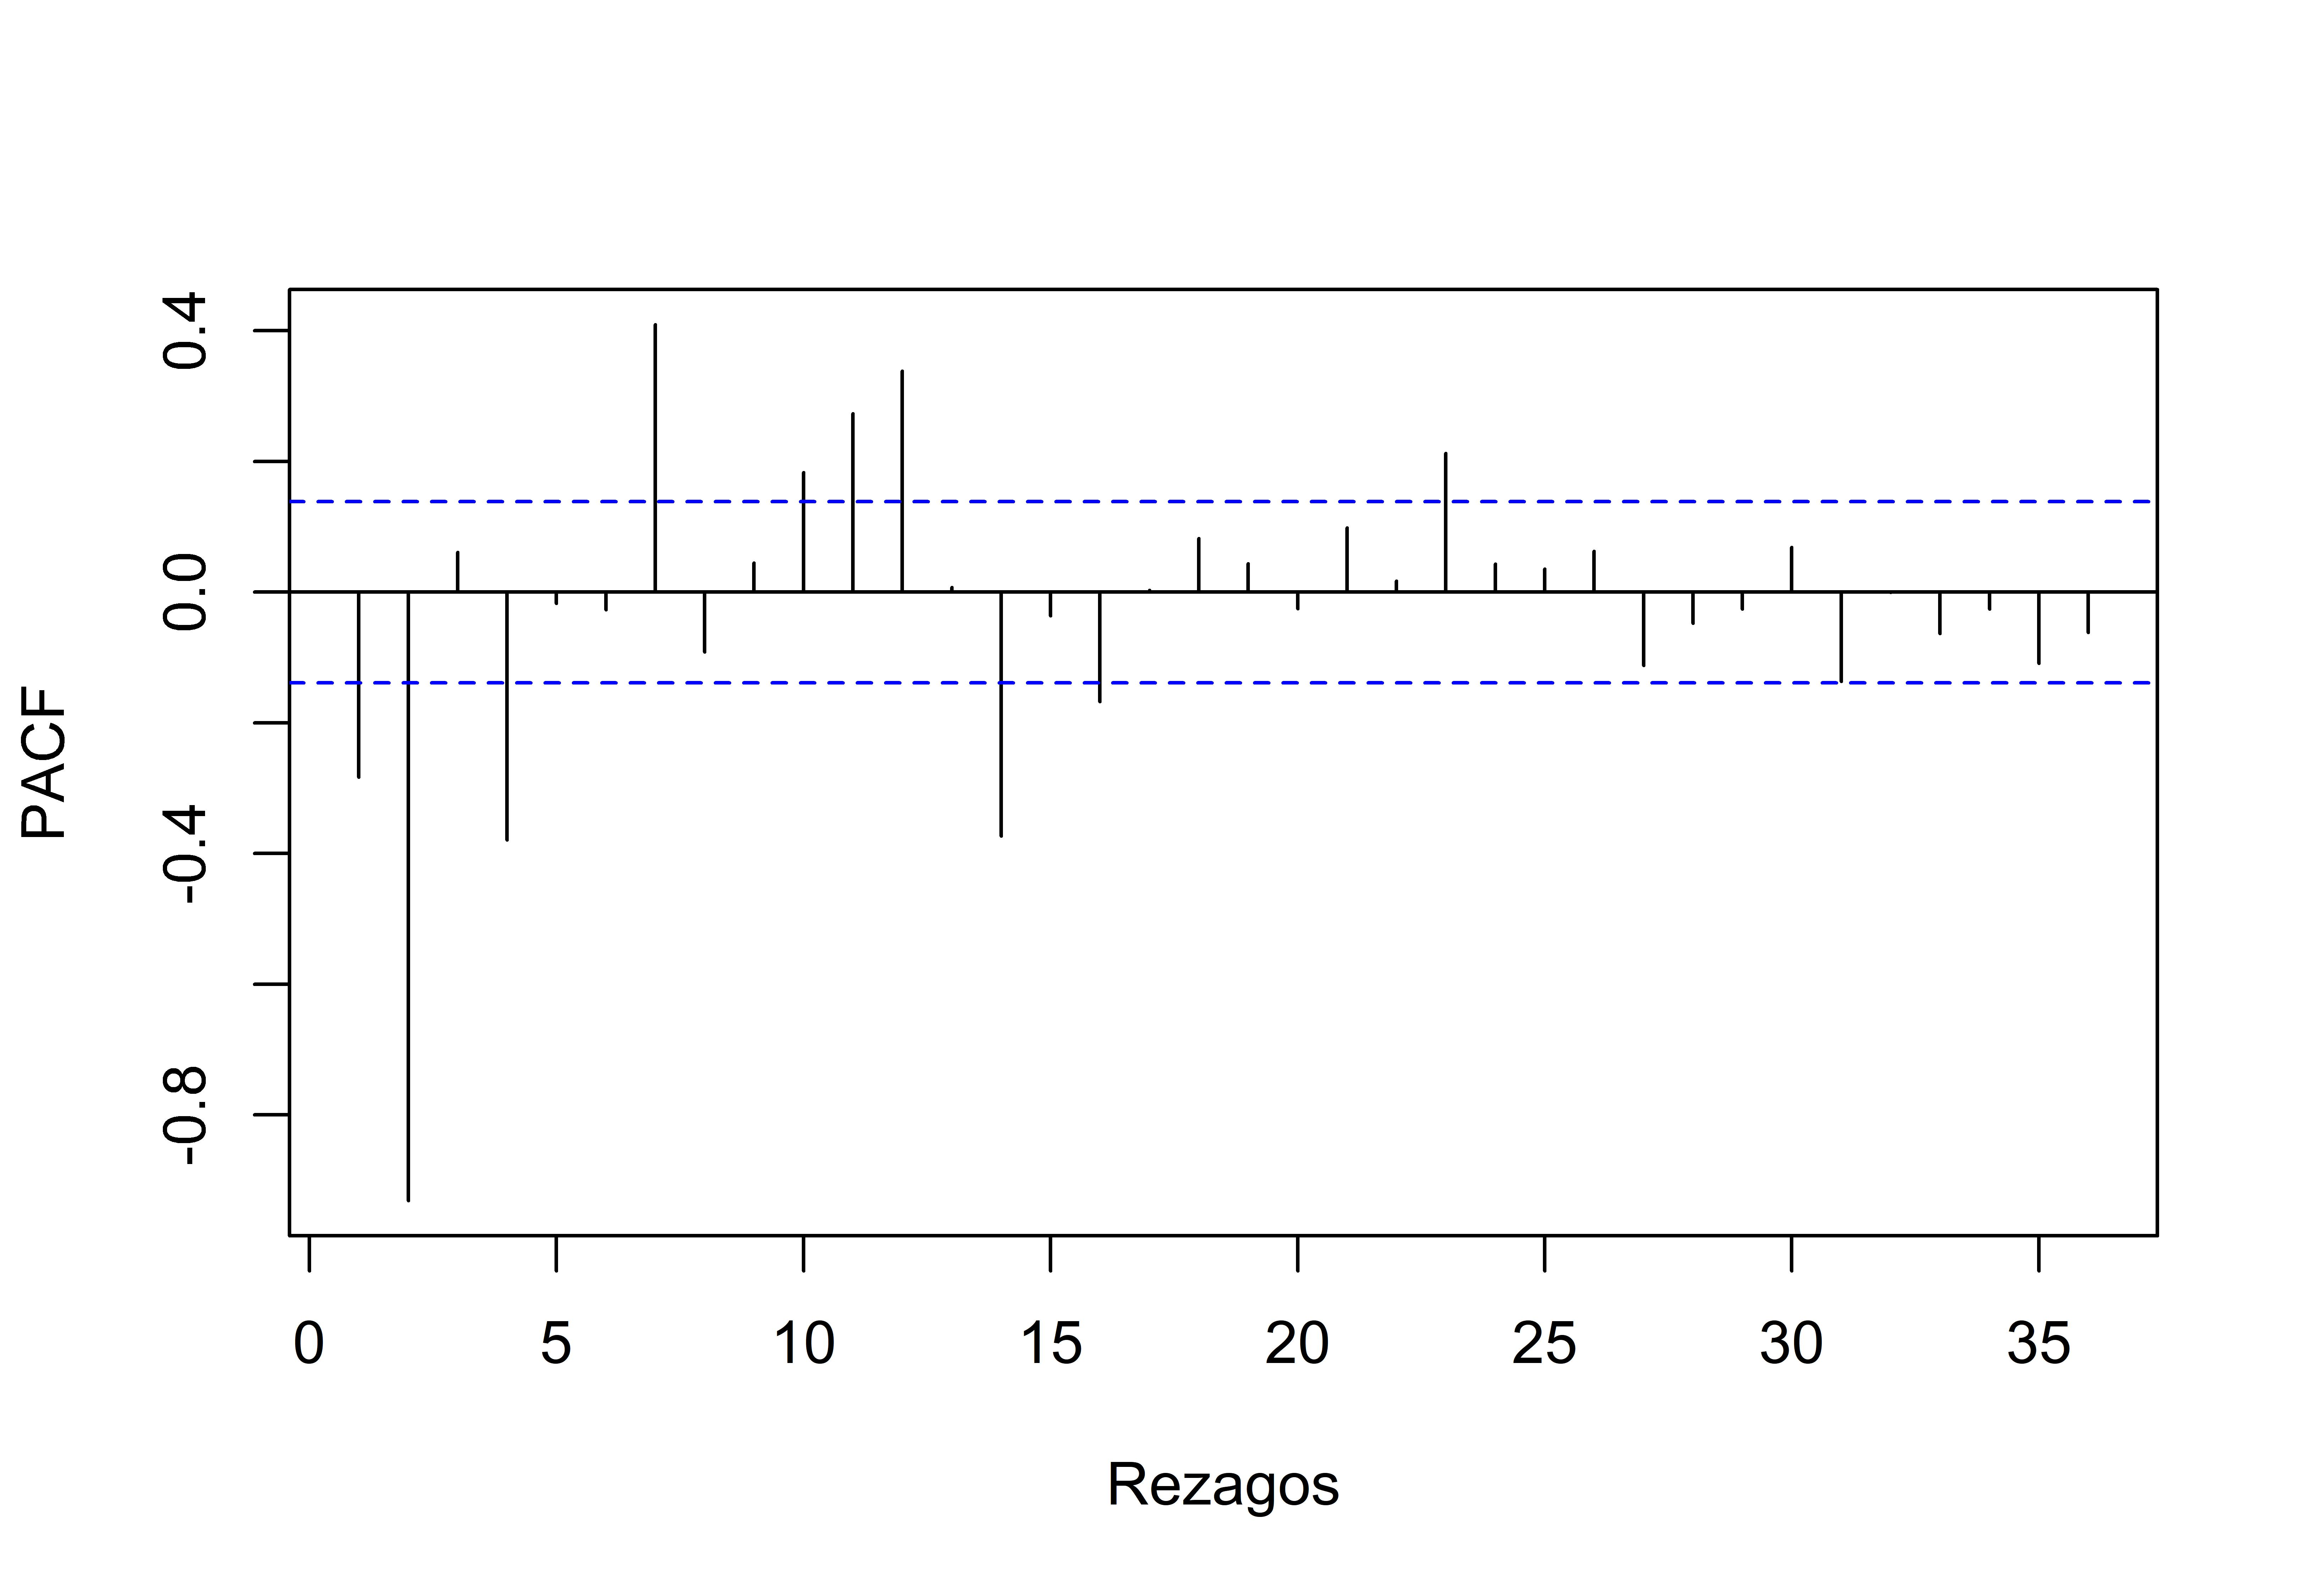
\includegraphics[width=1\linewidth,height=1\textheight]{Tesis_files/figure-latex/arima214_303_pacf-1} \caption{Autocorrelación parcial de los datos simulados a partir de un proceso ARIMA(2,1,4)(3,0,3)}\label{fig:arima214_303_pacf}
\end{figure}

\subsubsection{Tasa de mortalidad infantil interanual}

Como se mostró en la figura \ref{fig:tmiiplotgeneral}, la tasa de
mortalidad infantil interanual posee una tendencia claramente
decreciente, por lo que su media, por lo que no se trata de una serie
cronológica estacionaria. Tras aplicarle una diferenciación, esta
situación cambia, tal y como se muestra en la figura
\ref{fig:tmii_comportamiento}.

Por otro lado, las figuras \ref{fig:tmii_acf} y \ref{fig:tmii_pacf}
sugieren la presencia de procesos estacionales , mientras que en la
parte no estacional se observa como la \emph{ACF} va disminuyendo y el
\emph{PACF} se corta tras el segundo rezado, lo cual podría ser indicio
de un proceso \(MA(2)\) o superior.

\begin{figure}[H]
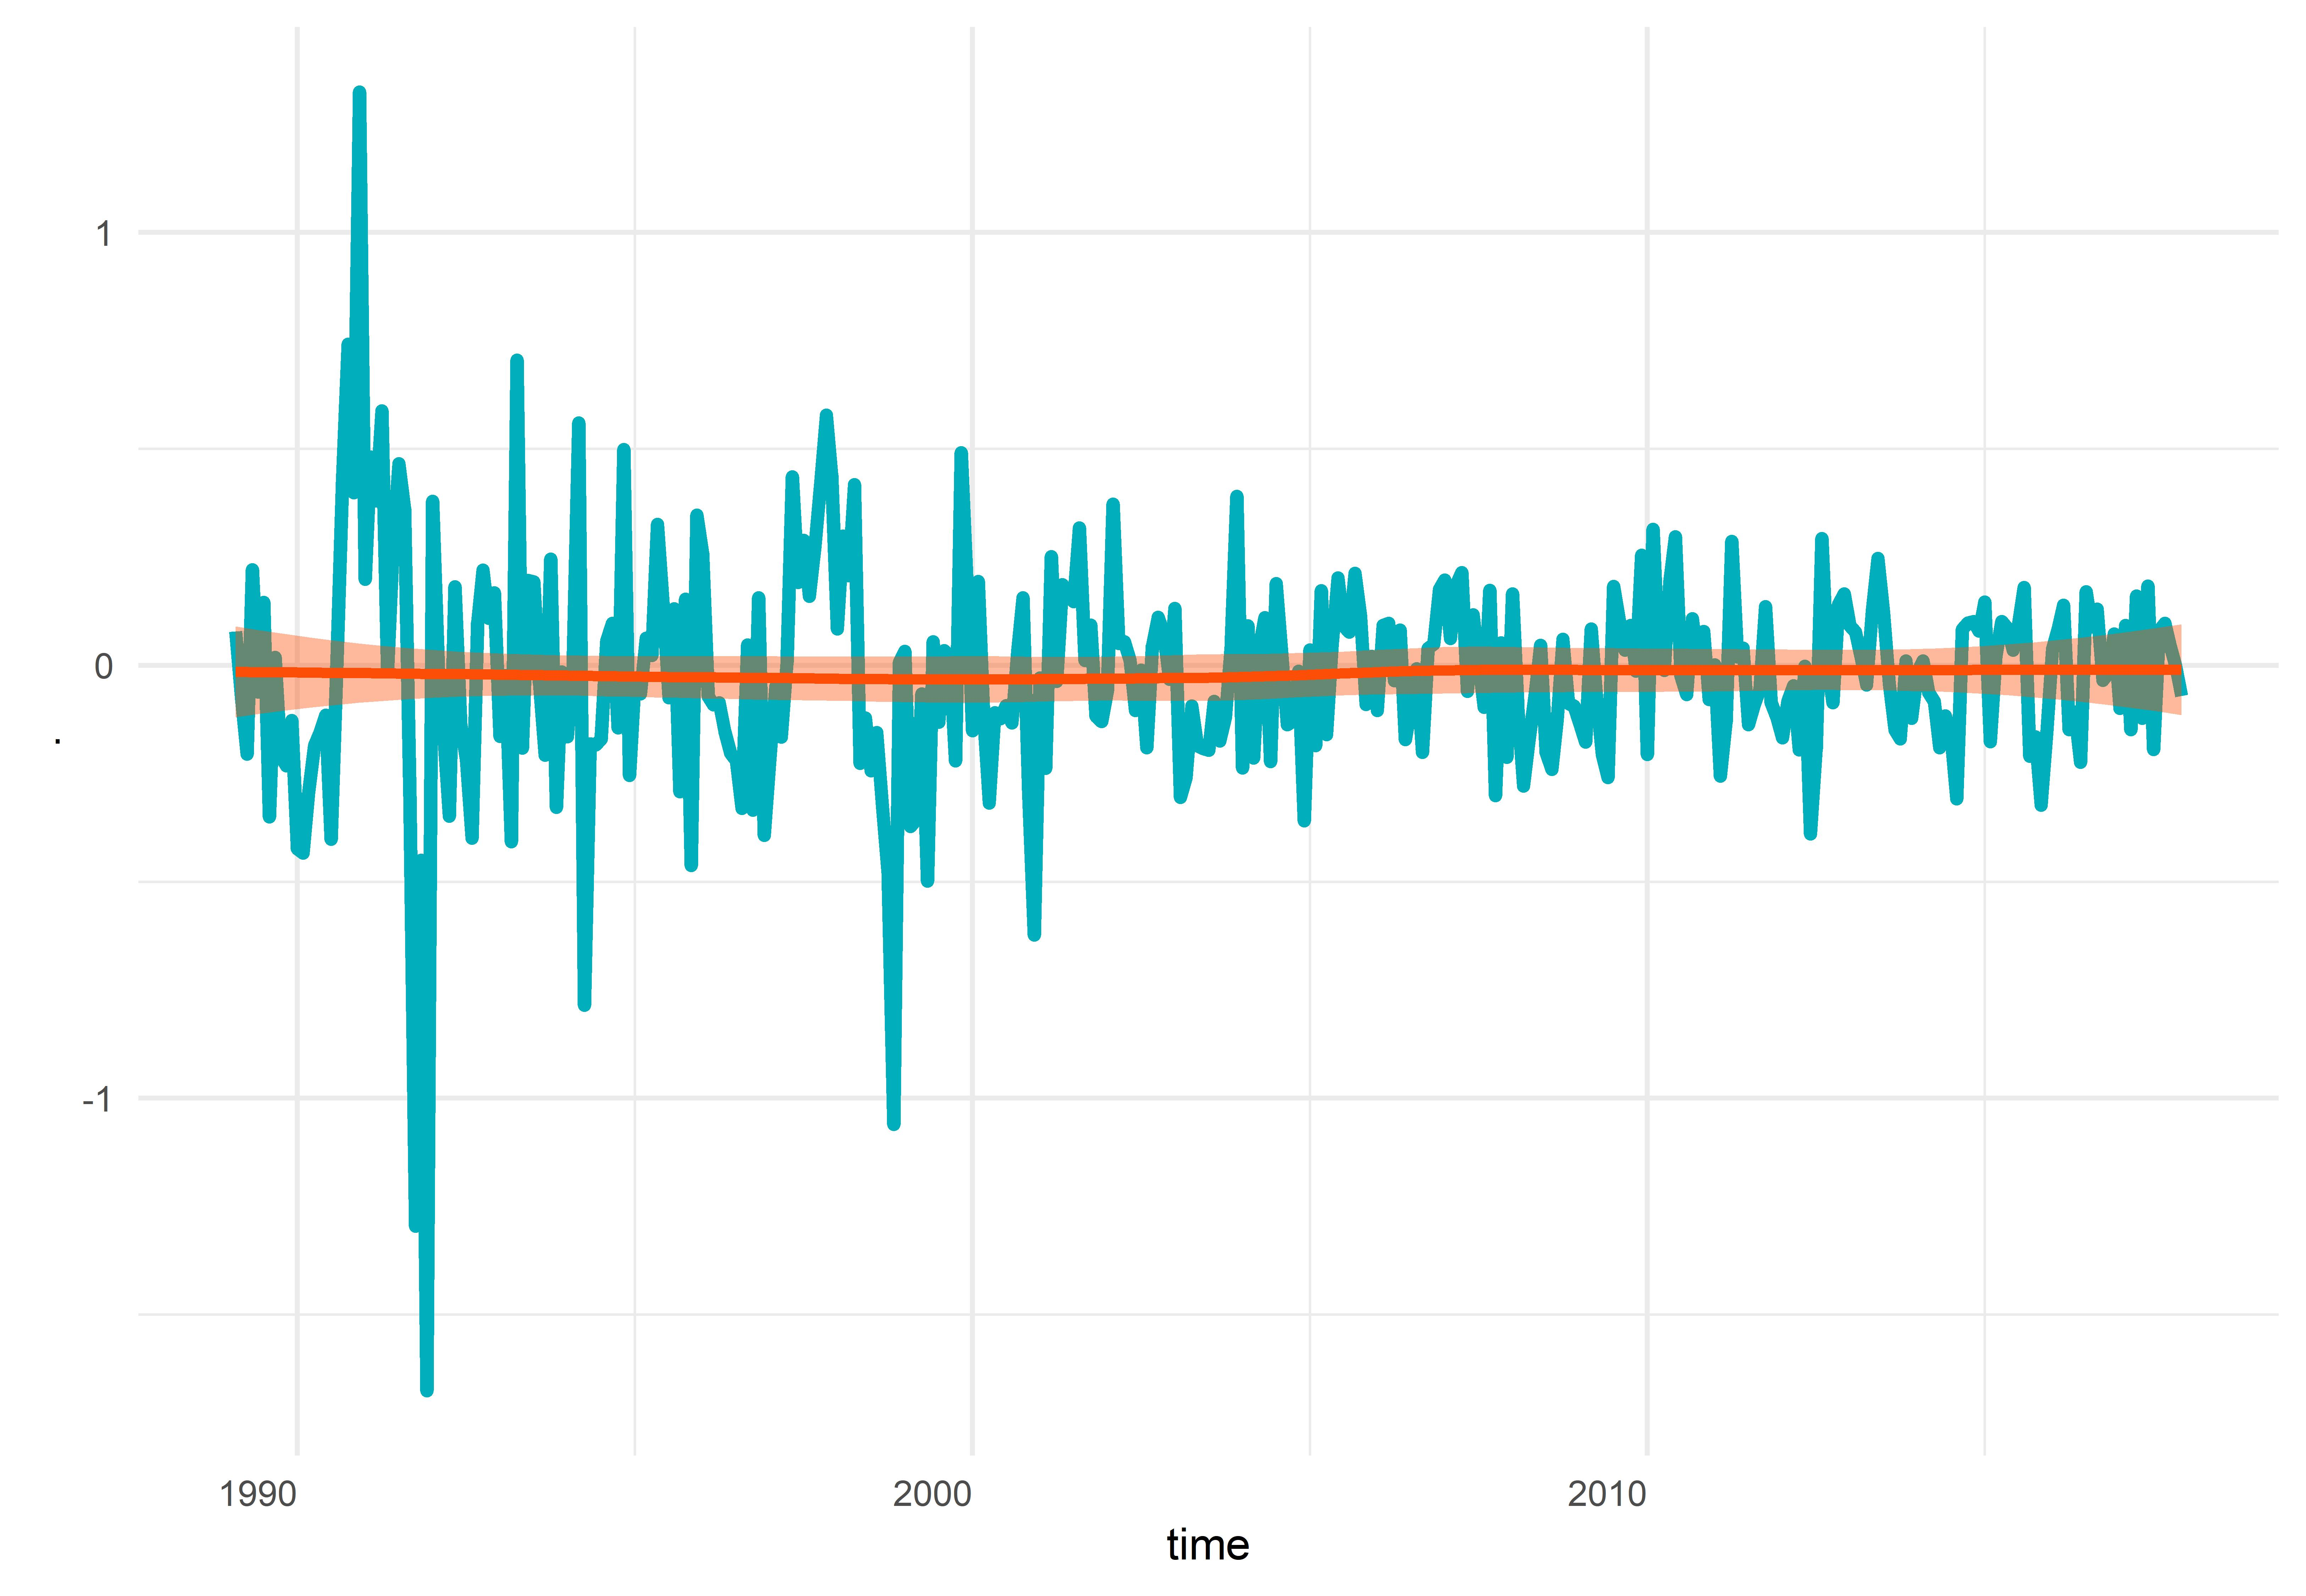
\includegraphics[width=1\linewidth,height=1\textheight]{Tesis_files/figure-latex/tmii_comportamiento-1} \caption{Tendencia de los datos diferenciados de la TMII}\label{fig:tmii_comportamiento}
\end{figure}

\begin{figure}[H]
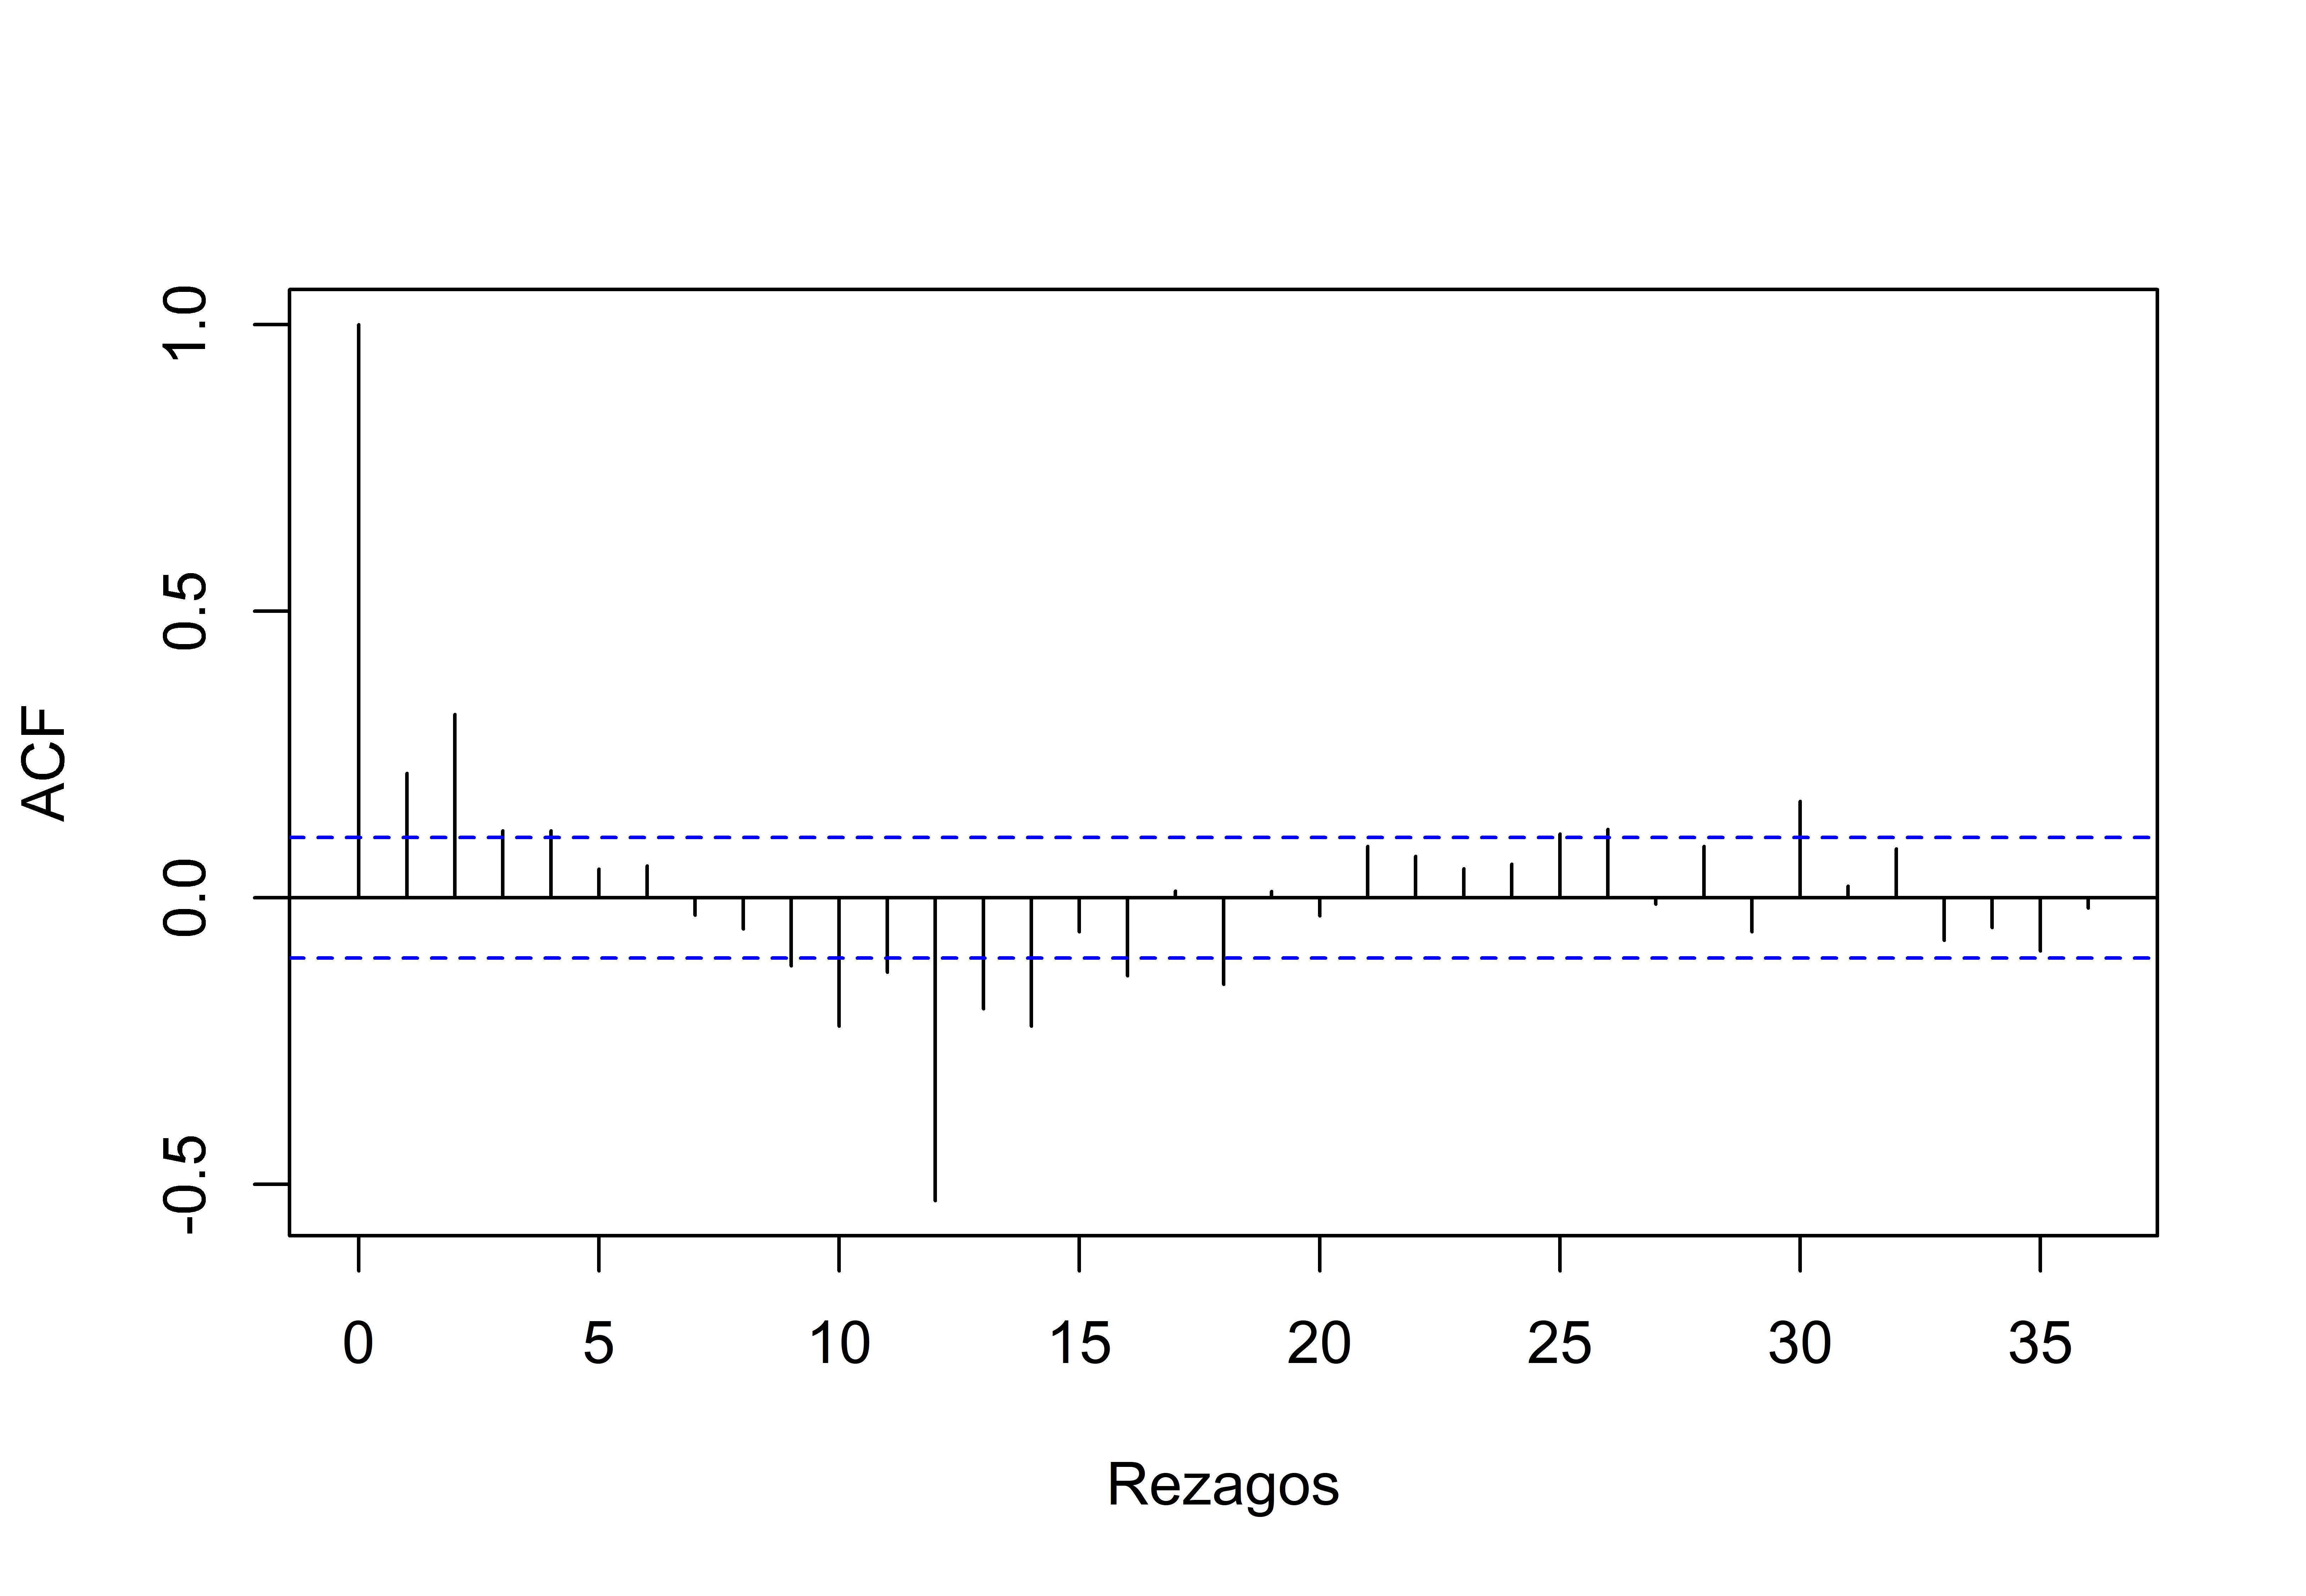
\includegraphics[width=1\linewidth,height=1\textheight]{Tesis_files/figure-latex/tmii_acf-1} \caption{Autocorrelación de los datos diferenciados de la TMII}\label{fig:tmii_acf}
\end{figure}

\begin{figure}[H]
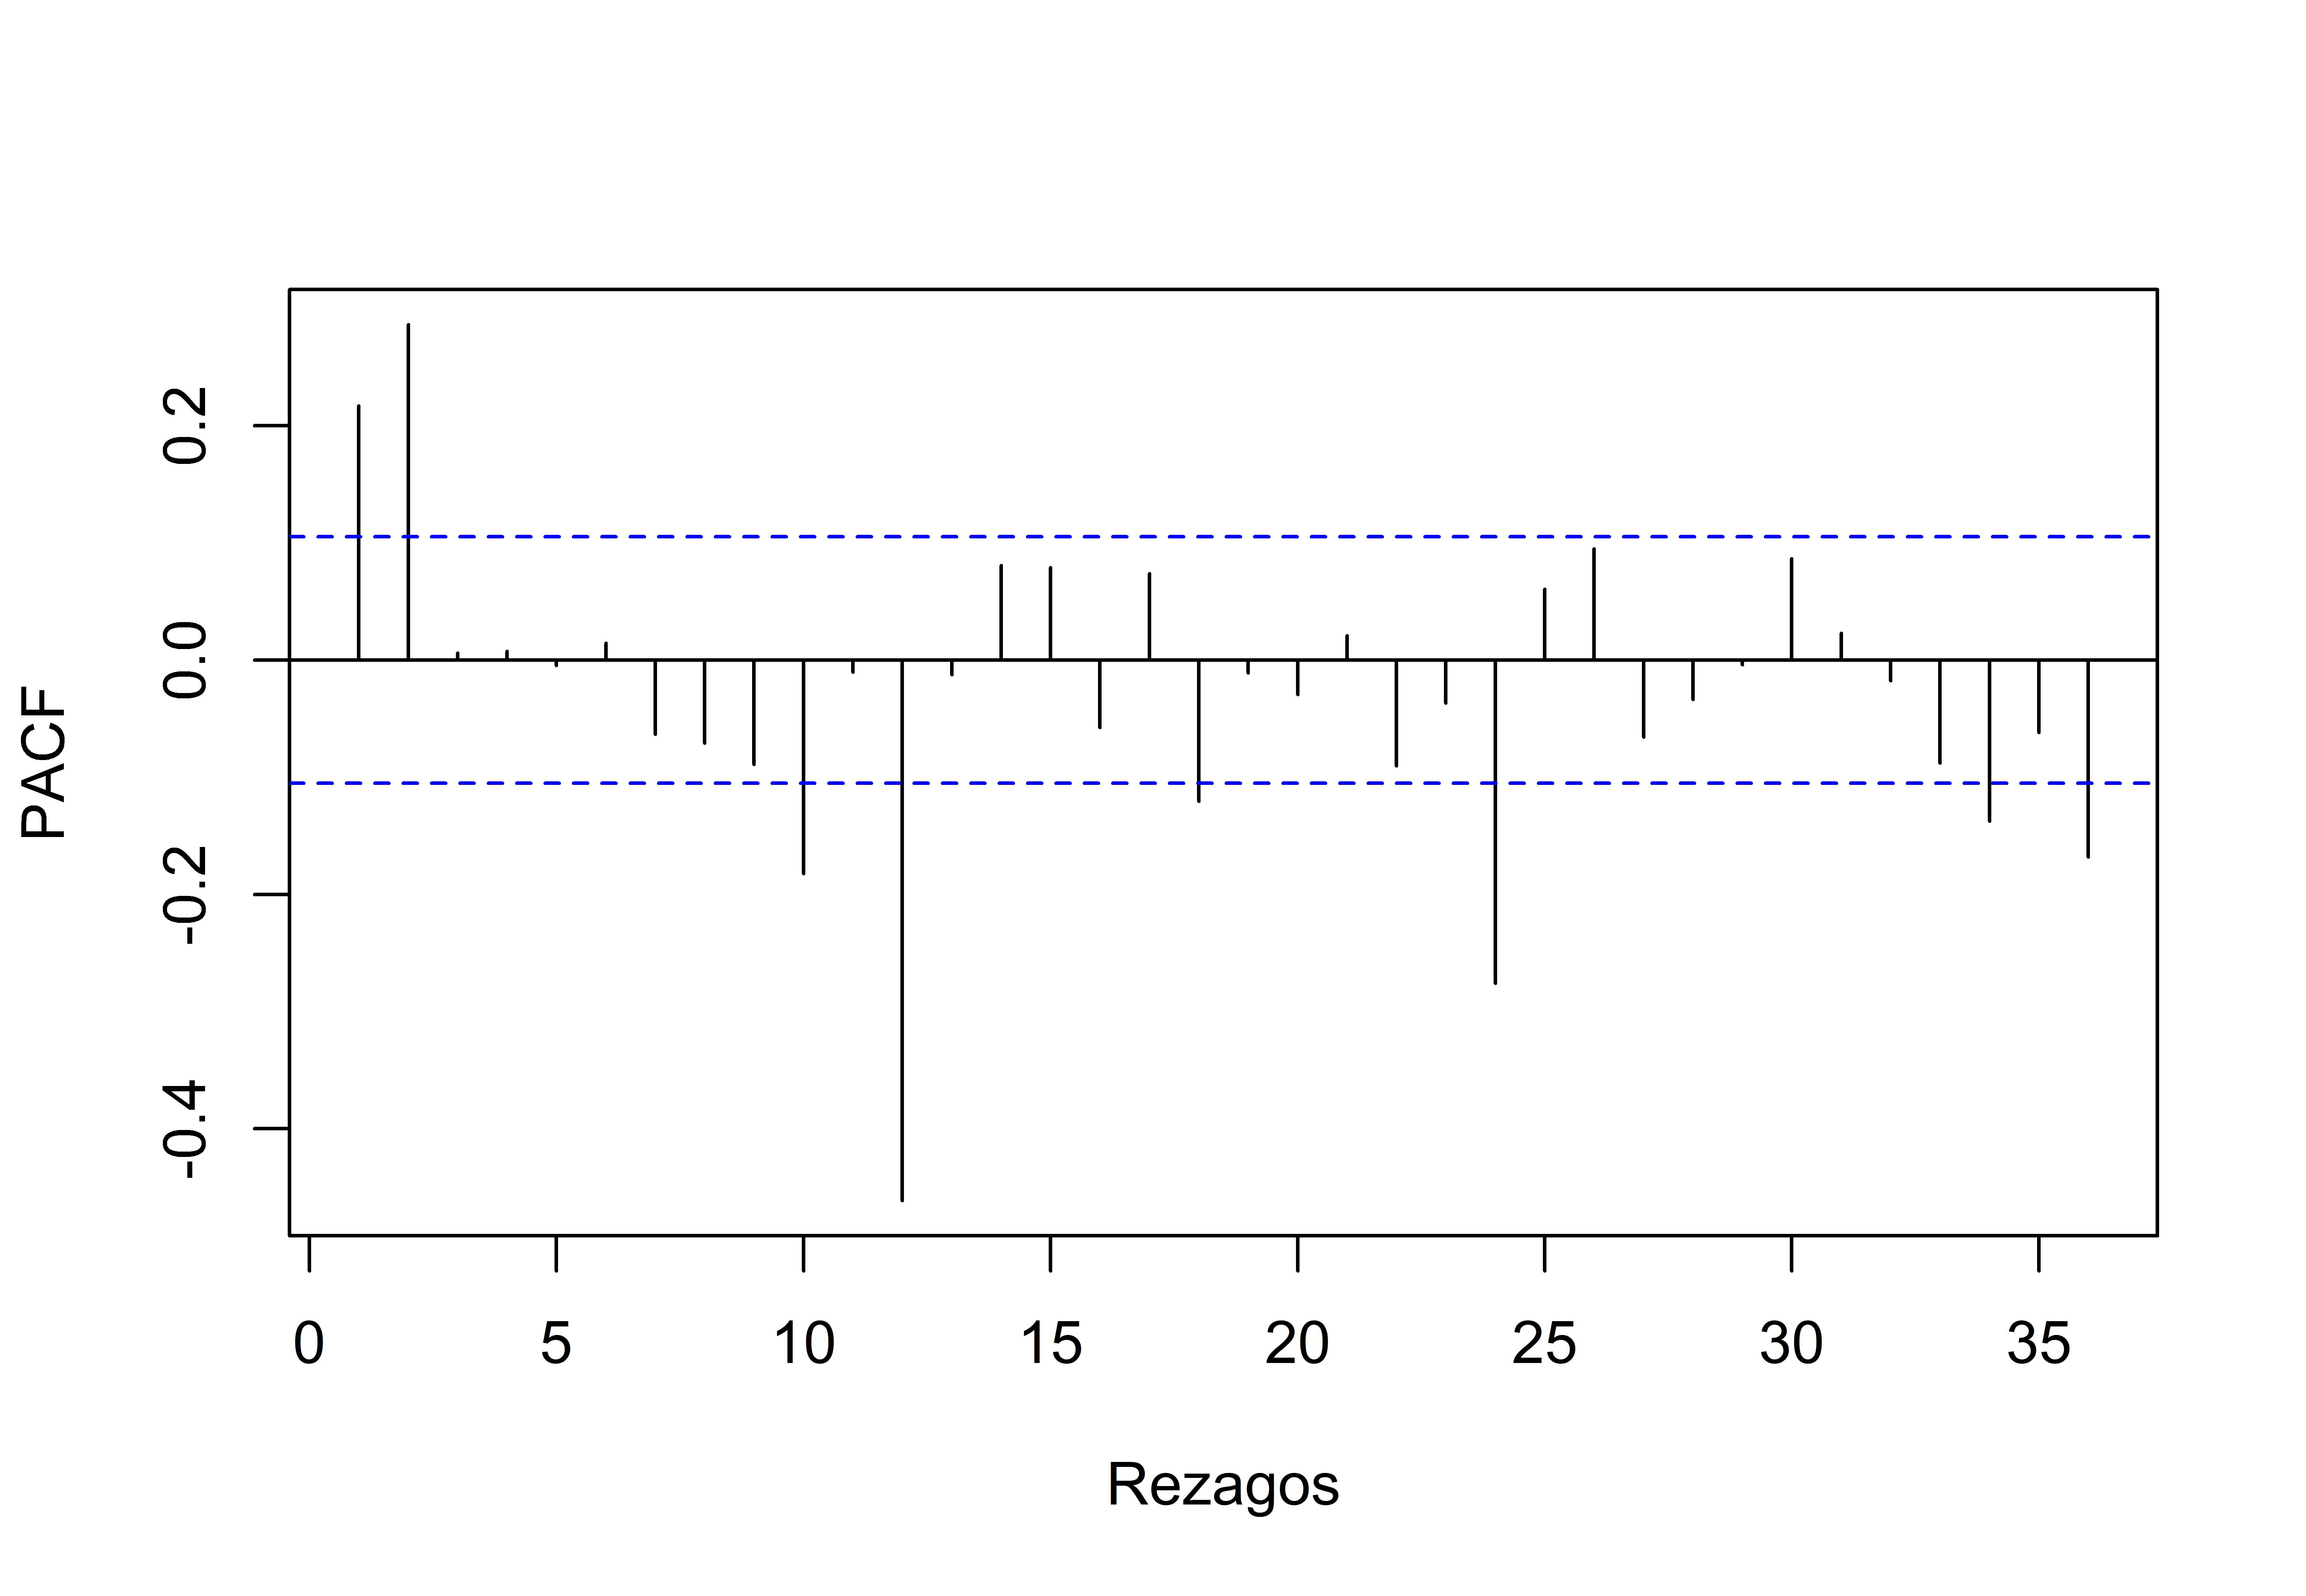
\includegraphics[width=1\linewidth,height=1\textheight]{Tesis_files/figure-latex/tmii_pacf-1} \caption{Autocorrelación parcial de los datos diferenciados de la TMII}\label{fig:tmii_pacf}
\end{figure}

\subsubsection{Mortalidad por causa externa}

En la figura \ref{fig:externaplotgeneral} se observó como la tasa de
mortalidad por causa externa posee una tendencia ligeramente creciente e
inestable a lo largo del tiempo, por lo que no se trata de una serie
cronológica estacionaria. Tras aplicarle una diferenciación la serie se
comporta como lo mostrado en la figura \ref{fig:externa_comportamiento}.
Además, las figuras \ref{fig:externa_acf} y \ref{fig:externa_pacf}
muestran indicios de un proceso bajo en la parte no estacional, y si
bien no hay indicios claros de patrones estacionales, es sabido que los
meses de Enero, Abril y Diciembre son los que cuentan con un mayor
número de defunciones por estas causas.

\begin{figure}[H]
\includegraphics[width=1\linewidth,height=1\textheight]{Tesis_files/figure-latex/externa_comportamiento-1} \caption{Tendencia de los datos diferenciados de la mortalidad por causa externa}\label{fig:externa_comportamiento}
\end{figure}

\begin{figure}[H]
\includegraphics[width=1\linewidth,height=1\textheight]{Tesis_files/figure-latex/externa_acf-1} \caption{Autocorrelación de los datos diferenciados de la mortalidad por causa externa}\label{fig:externa_acf}
\end{figure}

\begin{figure}[H]
\includegraphics[width=1\linewidth,height=1\textheight]{Tesis_files/figure-latex/externa_pacf-1} \caption{Autocorrelación parcial de los datos diferenciados de la mortalidad por causa externa}\label{fig:externa_pacf}
\end{figure}

\subsubsection{Incentivos salariales}

En la figura \ref{fig:incentivosplotgeneral} se observó como la serie de
incentivos salariales posee una tendencia creciente y sostenida a lo
largo del tiempo, por lo que no se trata de una serie cronológica
estacionaria. Tras una diferenciación la serie se comporta como lo
mostrado en la figura \ref{fig:incentivos_comportamiento}, que aunque su
media se mantiene constante, parece seguir teniendo patrones. Además,
las figuras \ref{fig:incentivos_acf} y \ref{fig:incentivos_pacf} no
parecen sugerir un proceso en particular tanto para la parte estacional
como para la no estacional, a pesar de que es claro que existe un efecto
periódico.

\begin{figure}[H]
\includegraphics[width=1\linewidth,height=1\textheight]{Tesis_files/figure-latex/incentivos_comportamiento-1} \caption{Tendencia de los datos diferenciados de la serie de incentivos salariales}\label{fig:incentivos_comportamiento}
\end{figure}

\begin{figure}[H]
\includegraphics[width=1\linewidth,height=1\textheight]{Tesis_files/figure-latex/incentivos_acf-1} \caption{Autocorrelación de los datos diferenciados de la serie de incentivos salariales}\label{fig:incentivos_acf}
\end{figure}

\begin{figure}[H]
\includegraphics[width=1\linewidth,height=1\textheight]{Tesis_files/figure-latex/incentivos_pacf-1} \caption{Autocorrelación parcial de los datos diferenciados de la serie de incentivos salariales}\label{fig:incentivos_pacf}
\end{figure}

\subsubsection{Intereses y comisiones del sector público}

En la figura \ref{fig:interesesplotgeneral} se muestra como la serie de
intereses y comisiones del sector público posee una tendencia creciente
no lineal, por lo que no se trata de una serie de tiempo estacionaria.
Tras utilizar una diferenciación la serie se comporta como lo mostrado
en la figura \ref{fig:intereses_comportamiento}, que aunque su media se
mantiene constante, pero aún conserva algunos patrones. Las figuras
\ref{fig:intereses_acf} y \ref{fig:intereses_pacf} indican que existen
un efecto estacional, pero su identificación no es clara.

\begin{figure}[H]
\includegraphics[width=1\linewidth,height=1\textheight]{Tesis_files/figure-latex/intereses_comportamiento-1} \caption{Tendencia de los datos diferenciados de la serie de intereses y comisiones del sector público}\label{fig:intereses_comportamiento}
\end{figure}

\begin{figure}[H]
\includegraphics[width=1\linewidth,height=1\textheight]{Tesis_files/figure-latex/intereses_acf-1} \caption{Autocorrelación de los datos diferenciados de la serie de intereses y comisiones del sector público}\label{fig:intereses_acf}
\end{figure}

\begin{figure}[H]
\includegraphics[width=1\linewidth,height=1\textheight]{Tesis_files/figure-latex/intereses_pacf-1} \caption{Autocorrelación parcial de los datos diferenciados de la serie de intereses y comisiones del sector público}\label{fig:intereses_pacf}
\end{figure}

\subsection{Partición de los datos}

Como se mencionó en la metodología, la partición utilizada consiste en
tomar 80\% de las observaciones para generar el serie cronológica de
entrenamiento para ajustar los modelos, mientras que el restante 20\%
corresponde al la serie cronológica utilizada como validación. En el
caso de los datos simulados, la ventana de observación de los datos
seleccionados se muestra en la figura
\ref{fig:particion_series_simuladas} para los datos simulados, y en la
figura \ref{fig:particion_series_reales} para las series de tiempo
reales.

\begin{figure}[H]
\includegraphics[width=1\linewidth,height=1\textheight]{Tesis_files/figure-latex/particion_series_simuladas-1} \caption{Partición de los datos en los conjuntos de entrenamiento y validación para las series de tiempo simuladas}\label{fig:particion_series_simuladas}
\end{figure}

\begin{figure}[H]
\includegraphics[width=1\linewidth,height=1\textheight]{Tesis_files/figure-latex/particion_series_reales-1} \caption{Partición de los datos en los conjuntos de entrenamiento y validación para las series de tiempo reales}\label{fig:particion_series_reales}
\end{figure}

\subsection{Identificación y estimación del mejor modelo según la función auto.arima()}

Al ajustar modelos con la función \texttt{auto.arima()}, al igual que
con cualquier otro método para estimar modelos \(ARIMA\), se obtienen
estimaciones de coeficientes. En el caso de los datos simulados, donde
se conoce el verdadero proceso que gobierna la serie de tiempo, estos
valores pueden compararse con los valores obtenidos.

\subsubsection{Datos simulados}

El cuadro \ref{tab:coeficientes_original_autoarima} resume los
resultados obtenidos en la estimación de los coeficientes. En la columna
\emph{Proceso original} se indica el proceso a partir del cual se generó
la serie cronológica mediante simulación, en la columna
\emph{Coeficiente} se indica el coeficiente al cual pertenecen las
estimaciones presentes en las columnas \emph{Valor real} (el valor del
coeficiente del proceso original), \emph{Estimación auto.arima()} (valor
estimado del coeficiente mediante la función \texttt{auto.arima()}),
\emph{Límite Inferior} y \emph{Límite Superior} del intervalo de
confianza el 95\% para los coeficientes estimados en la columna
\emph{Estimación auto.arima()}. Como se ha mencionado, la notación más
utilizada para los modelos \(ARIMA\) es \(ARIMA(p,d,q)(P,D,Q)\), que en
la columna \emph{Coeficiente} equivale a
\(ARIMA(ARX, d, MAX)(SARX, D, SMAX)\), con \(X=\{1,2,3,4\}\), según
corresponda.

De esta manera, a modo de ejemplo, para los datos simulados a partir de
un \(ARIMA(4,0,2)\), los coeficientes de \(AR1\) hasta \(AR4\)
representan los cuatro coeficientes de la parte autorregresiva no
estacional, mientras que \(MA1\) y \(MA2\) son los dos coeficientes del
modelo de medias móviles de la parte no estacional, la celda del
\emph{Valor real} correspondiente al coeficiente \(MA3\) está vacía
porque el modelo original solo tenía dos coeficientes en el modelo de
medias móviles, no tres. Así, el modelo estimado con
\texttt{auto.arima()} estima únicamente los coeficientes \(AR1\) y
\(AR2\) para el modelo autorregresivo, y \(MA1\), \(MA2\) y \(MA3\) para
el modelo de medias móviles.

\begin{table}[!h]

\caption{\label{tab:unnamed-chunk-25}\label{tab:coeficientes_original_autoarima}Coefcientes del proceso original y los estimados con auto.arima()}
\centering
\resizebox{\linewidth}{!}{
\fontsize{5}{7}\selectfont
\begin{tabu} to \linewidth {>{}r>{\raggedleft\arraybackslash}p{2.5cm}>{\raggedleft}X>{\raggedleft}X>{\raggedleft}X>{\raggedleft}X}
\toprule
Proceso original & Coeficiente & Valor real & Estimación auto.arima() & Límite Inferior & Límite Superior\\
\midrule
\textbf{} & AR1 & 0.49 & 0.39 & 0.22 & 0.57\\
\cmidrule{2-6}
\textbf{} & AR2 &  & -0.11 & -0.28 & 0.06\\
\cmidrule{2-6}
\textbf{\multirow{-3}{2.5cm}{\raggedleft\arraybackslash ARIMA(1,0,0)}} & MA1 &  & -0.92 & -1.02 & -0.82\\
\cmidrule{1-6}
\textbf{} & AR1 & 0.94 &  &  & \\
\cmidrule{2-6}
\textbf{\multirow{-2}{2.5cm}{\raggedleft\arraybackslash ARIMA(1,0,1)}} & MA1 & 0.55 & 0.73 & 0.63 & 0.82\\
\cmidrule{1-6}
\textbf{} & AR1 & 0.34 & 0.46 & 0.27 & 0.65\\
\cmidrule{2-6}
\textbf{} & AR2 & 0.19 &  &  & \\
\cmidrule{2-6}
\textbf{} & MA1 & -0.41 & -0.3 & -0.5 & -0.11\\
\cmidrule{2-6}
\textbf{} & MA2 & 0.42 & 0.15 & -0.03 & 0.32\\
\cmidrule{2-6}
\textbf{\multirow{-5}{2.5cm}{\raggedleft\arraybackslash ARIMA(2,0,3)}} & MA3 & 0.97 & 0.66 & 0.46 & 0.85\\
\cmidrule{1-6}
\textbf{} & AR1 & -0.02 & -0.81 & -0.94 & -0.69\\
\cmidrule{2-6}
\textbf{} & AR2 & 0.29 &  &  & \\
\cmidrule{2-6}
\textbf{} & AR3 & 0.04 &  &  & \\
\cmidrule{2-6}
\textbf{} & AR4 & 0.57 &  &  & \\
\cmidrule{2-6}
\textbf{} & MA1 & 0.04 & -0.09 & -0.3 & 0.11\\
\cmidrule{2-6}
\textbf{} & MA2 & 0.8 & 0.29 & 0.12 & 0.47\\
\cmidrule{2-6}
\textbf{\multirow{-7}{2.5cm}{\raggedleft\arraybackslash ARIMA(4,0,2)}} & MA3 &  & -0.21 & -0.41 & -0.01\\
\cmidrule{1-6}
\textbf{} & MA1 & 0.55 & 0.59 & 0.45 & 0.72\\
\cmidrule{2-6}
\textbf{\multirow{-2}{2.5cm}{\raggedleft\arraybackslash ARIMA(0,0,1)(0,1,1)}} & SMA1 & 0.41 & 0.32 & 0.15 & 0.5\\
\cmidrule{1-6}
\textbf{} & AR1 & 0.01 & 0.82 & 0.69 & 0.95\\
\cmidrule{2-6}
\textbf{} & AR2 & 0.56 &  &  & \\
\cmidrule{2-6}
\textbf{} & MA1 & -0.72 & -1.07 & -1.27 & -0.88\\
\cmidrule{2-6}
\textbf{} & MA2 & 0.03 & 0.49 & 0.3 & 0.68\\
\cmidrule{2-6}
\textbf{} & MA3 & 0.89 &  &  & \\
\cmidrule{2-6}
\textbf{} & MA4 & 0.79 &  &  & \\
\cmidrule{2-6}
\textbf{} & SAR1 & 0.37 & -0.99 & -1.2 & -0.78\\
\cmidrule{2-6}
\textbf{} & SAR2 & 0.38 & -0.57 & -0.71 & -0.44\\
\cmidrule{2-6}
\textbf{} & SAR3 & 0.09 &  &  & \\
\cmidrule{2-6}
\textbf{} & SMA1 & 0.42 & 0.68 & 0.43 & 0.92\\
\cmidrule{2-6}
\textbf{} & SMA2 & -0.07 &  &  & \\
\cmidrule{2-6}
\textbf{\multirow{-12}{2.5cm}{\raggedleft\arraybackslash ARIMA(2,1,4)(3,0,3)}} & SMA3 & 0.55 &  &  & \\
\bottomrule
\end{tabu}}
\end{table}

\subsubsection{Datos reales}

En el caso de las series cronológicas reales, se toma en consideración
el mejor modelo sugerido por la función \texttt{auto.arima()}. Los
coeficientes obtenidos para las distintas series de tiempo
costarricenses se muestran en el cuadro
\ref{tab:coeficientes_reales_autoarima}.

\begin{table}[!h]

\caption{\label{tab:unnamed-chunk-26}\label{tab:coeficientes_reales_autoarima}Coefcientes de los modelos ajustados con a las series reales con auto.arima()}
\centering
\resizebox{\linewidth}{!}{
\fontsize{5}{7}\selectfont
\begin{tabu} to \linewidth {>{}r>{\raggedleft\arraybackslash}p{2.5cm}>{\raggedleft}X>{\raggedleft}X>{\raggedleft}X}
\toprule
Serie & Coeficiente & Estimación & Límite Inferior & Límite Superior\\
\midrule
\textbf{} & AR1 & 0.19 & 0.08 & 0.31\\
\cmidrule{2-5}
\textbf{} & AR2 & 0.32 & 0.21 & 0.44\\
\cmidrule{2-5}
\textbf{\multirow{-3}{2.5cm}{\raggedleft\arraybackslash TMII}} & SMA1 & -0.78 & -0.87 & -0.69\\
\cmidrule{1-5}
\textbf{} & AR1 & -0.11 & -0.29 & 0.08\\
\cmidrule{2-5}
\textbf{\multirow{-2}{2.5cm}{\raggedleft\arraybackslash Mortalidad por causa externa}} & MA1 & -0.82 & -0.94 & -0.70\\
\cmidrule{1-5}
\textbf{} & MA1 & 0.22 & -0.06 & 0.49\\
\cmidrule{2-5}
\textbf{\multirow{-2}{2.5cm}{\raggedleft\arraybackslash Incentivos salariales}} & SAR1 & 0.54 & 0.31 & 0.76\\
\cmidrule{1-5}
\textbf{Intereses y comisiones} & MA1 & -0.44 & -0.62 & -0.27\\
\bottomrule
\end{tabu}}
\end{table}

\subsection{Identificación y estimación del mejor modelo con sobreparametrización}

De manera análoga al procedimiento realizado con la función
\texttt{auto.arima()}, se realiza el proceso descrito en la metodología
para seleccionar el mejor modelo utilizando la sobreparametrización.
Nuevamente, para los datos simulados, se conoce de previo el verdadero
proceso que gobierna la serie de temporal, los cuales se comparan con
los valores de los coeficientes de cada modelo obtenido mediante la
sobreparametrización.

\subsubsection{Datos simulados}

Los mismos conceptos explicados para el cuadro
\ref{tab:coeficientes_original_autoarima} aplican ahora para el
\ref{tab:coeficientes_original_sobreparametrizacion}.

\begin{table}[!h]

\caption{\label{tab:unnamed-chunk-27}\label{tab:coeficientes_original_sobreparametrizacion}Coefcientes del proceso original y los estimados con sobreparametrización}
\centering
\resizebox{\linewidth}{!}{
\fontsize{5}{7}\selectfont
\begin{tabu} to \linewidth {>{}r>{\raggedleft\arraybackslash}p{2.5cm}>{\raggedleft}X>{\raggedleft}X>{\raggedleft}X>{\raggedleft}X}
\toprule
Proceso original & Coeficiente & Valor real & Estimación sobreparametrización & Límite Inferior & Límite Superior\\
\midrule
\textbf{ARIMA(1,0,0)} & AR1 & 0.49 & 0.44 & 0.3 & 0.58\\
\cmidrule{1-6}
\textbf{} & AR1 & 0.94 &  &  & \\
\cmidrule{2-6}
\textbf{\multirow{-2}{2.5cm}{\raggedleft\arraybackslash ARIMA(1,0,1)}} & MA1 & 0.55 & 0.73 & 0.63 & 0.82\\
\cmidrule{1-6}
\textbf{} & AR1 & 0.34 &  &  & \\
\cmidrule{2-6}
\textbf{} & AR2 & 0.19 &  &  & \\
\cmidrule{2-6}
\textbf{} & MA1 & -0.41 & 0.15 & 0.01 & 0.3\\
\cmidrule{2-6}
\textbf{} & MA2 & 0.42 & 0.35 & 0.21 & 0.49\\
\cmidrule{2-6}
\textbf{} & MA3 & 0.97 & 0.74 & 0.62 & 0.85\\
\cmidrule{2-6}
\textbf{} & MA4 &  & 0.26 & 0.09 & 0.42\\
\cmidrule{2-6}
\textbf{\multirow{-7}{2.5cm}{\raggedleft\arraybackslash ARIMA(2,0,3)}} & MA5 &  & 0.36 & 0.2 & 0.51\\
\cmidrule{1-6}
\textbf{} & AR1 & -0.02 & -0.91 & -0.97 & -0.85\\
\cmidrule{2-6}
\textbf{} & AR2 & 0.29 &  &  & \\
\cmidrule{2-6}
\textbf{} & AR3 & 0.04 &  &  & \\
\cmidrule{2-6}
\textbf{} & AR4 & 0.57 &  &  & \\
\cmidrule{2-6}
\textbf{} & MA1 & 0.04 &  &  & \\
\cmidrule{2-6}
\textbf{\multirow{-6}{2.5cm}{\raggedleft\arraybackslash ARIMA(4,0,2)}} & MA2 & 0.8 &  &  & \\
\cmidrule{1-6}
\textbf{} & MA1 & 0.55 & 0.59 & 0.45 & 0.72\\
\cmidrule{2-6}
\textbf{\multirow{-2}{2.5cm}{\raggedleft\arraybackslash ARIMA(0,0,1)(0,1,1)}} & SMA1 & 0.41 & 0.32 & 0.15 & 0.5\\
\cmidrule{1-6}
\textbf{} & AR1 & 0.01 & 0.81 & 0.68 & 0.95\\
\cmidrule{2-6}
\textbf{} & AR2 & 0.56 &  &  & \\
\cmidrule{2-6}
\textbf{} & MA1 & -0.72 & -1.07 & -1.25 & -0.88\\
\cmidrule{2-6}
\textbf{} & MA2 & 0.03 & 0.51 & 0.33 & 0.69\\
\cmidrule{2-6}
\textbf{} & MA3 & 0.89 &  &  & \\
\cmidrule{2-6}
\textbf{} & MA4 & 0.79 &  &  & \\
\cmidrule{2-6}
\textbf{} & SAR1 & 0.37 & -1.09 & -1.27 & -0.91\\
\cmidrule{2-6}
\textbf{} & SAR2 & 0.38 & -0.83 & -1.02 & -0.64\\
\cmidrule{2-6}
\textbf{} & SAR3 & 0.09 &  &  & \\
\cmidrule{2-6}
\textbf{} & SMA1 & 0.42 & 0.84 & 0.54 & 1.15\\
\cmidrule{2-6}
\textbf{} & SMA2 & -0.07 & 0.4 & 0.05 & 0.76\\
\cmidrule{2-6}
\textbf{\multirow{-12}{2.5cm}{\raggedleft\arraybackslash ARIMA(2,1,4)(3,0,3)}} & SMA3 & 0.55 &  &  & \\
\bottomrule
\end{tabu}}
\end{table}

\subsubsection{Datos reales}

Para las series cronológicas reales también se toma en consideración el
mejor modelo sugerido esta vez por la sobreparametrización. Los
coeficientes obtenidos para las distintas series de tiempo
costarricenses se muestran en el cuadro
\ref{tab:coeficientes_reales_sobreparametrizacion}.

\begin{table}[!h]

\caption{\label{tab:unnamed-chunk-28}\label{tab:coeficientes_reales_sobreparametrizacion}Coefcientes de los modelos ajustados con a las series reales con sobreparametrización}
\centering
\resizebox{\linewidth}{!}{
\fontsize{5}{7}\selectfont
\begin{tabu} to \linewidth {>{}r>{\raggedleft\arraybackslash}p{2.5cm}>{\raggedleft}X>{\raggedleft}X>{\raggedleft}X}
\toprule
Serie & Coeficiente & Estimación & Límite Inferior & Límite Superior\\
\midrule
\textbf{} & AR1 & -0.39 & -0.40 & -0.38\\
\cmidrule{2-5}
\textbf{} & AR2 & 0.49 & 0.48 & 0.50\\
\cmidrule{2-5}
\textbf{} & AR3 & 0.73 & 0.73 & 0.73\\
\cmidrule{2-5}
\textbf{} & AR4 & 0.17 & 0.17 & 0.17\\
\cmidrule{2-5}
\textbf{} & MA1 & 1.51 & 1.46 & 1.56\\
\cmidrule{2-5}
\textbf{} & MA2 & 1.32 & 1.30 & 1.33\\
\cmidrule{2-5}
\textbf{} & MA3 & 0.61 & 0.58 & 0.64\\
\cmidrule{2-5}
\textbf{} & MA4 & 0.21 & 0.21 & 0.22\\
\cmidrule{2-5}
\textbf{} & SAR1 & -0.99 & -0.99 & -0.98\\
\cmidrule{2-5}
\textbf{} & SAR2 & -0.52 & -0.53 & -0.52\\
\cmidrule{2-5}
\textbf{} & SAR3 & -0.29 & -0.29 & -0.28\\
\cmidrule{2-5}
\textbf{} & SAR4 & -0.21 & -0.22 & -0.20\\
\cmidrule{2-5}
\textbf{} & SMA1 & -0.69 & -0.71 & -0.68\\
\cmidrule{2-5}
\textbf{} & SMA2 & -0.46 & -0.47 & -0.45\\
\cmidrule{2-5}
\textbf{} & SMA3 & 0.12 & 0.11 & 0.13\\
\cmidrule{2-5}
\textbf{\multirow{-16}{2.5cm}{\raggedleft\arraybackslash TMII}} & SMA4 & 0.14 & 0.13 & 0.15\\
\cmidrule{1-5}
\textbf{} & AR1 & 0.71 & 0.45 & 0.97\\
\cmidrule{2-5}
\textbf{} & AR2 & 0.24 & 0.04 & 0.44\\
\cmidrule{2-5}
\textbf{} & MA1 & -0.72 & -0.95 & -0.48\\
\cmidrule{2-5}
\textbf{\multirow{-4}{2.5cm}{\raggedleft\arraybackslash Mortalidad por causa externa}} & SMA1 & -1.00 & -1.29 & -0.71\\
\cmidrule{1-5}
\textbf{} & AR1 & -0.57 & -0.78 & -0.37\\
\cmidrule{2-5}
\textbf{} & AR2 & -0.50 & -0.71 & -0.29\\
\cmidrule{2-5}
\textbf{} & SAR1 & 0.43 & 0.14 & 0.72\\
\cmidrule{2-5}
\textbf{\multirow{-4}{2.5cm}{\raggedleft\arraybackslash Incentivos salariales}} & SAR2 & 0.35 & 0.04 & 0.65\\
\cmidrule{1-5}
\textbf{} & MA1 & -1.45 & -1.63 & -1.27\\
\cmidrule{2-5}
\textbf{\multirow{-2}{2.5cm}{\raggedleft\arraybackslash Intereses y comisiones}} & MA2 & 0.49 & 0.31 & 0.67\\
\bottomrule
\end{tabu}}
\end{table}

\subsection{Estimación de un modelo ARIMA estándar}

Ajustar un modelo ARIMA genérico sirve para referenciar los demás
resultados obtenidos, es decir, contrastarlos con los resultados del
\texttt{auto.arima()} y la sobreparametrización. Nuevamente, para los
datos simulados se comparan los coeficientes obtenidos con los que se
connocen a priori.

\subsubsection{Datos simulados}

Los mismos conceptos explicados para los cuadros
\ref{tab:coeficientes_original_autoarima} y
\ref{tab:coeficientes_original_sobreparametrizacion} aplican ahora para
el cuadro \ref{tab:coeficientes_original_arima_estandar}.

\begin{table}[!h]

\caption{\label{tab:unnamed-chunk-29}\label{tab:coeficientes_original_arima_estandar}Coefcientes del proceso original y los estimados con un ARIMA estándar}
\centering
\resizebox{\linewidth}{!}{
\fontsize{5}{7}\selectfont
\begin{tabu} to \linewidth {>{}r>{\raggedleft\arraybackslash}p{2.5cm}>{\raggedleft}X>{\raggedleft}X>{\raggedleft}X>{\raggedleft}X}
\toprule
Proceso original & Coeficiente & Valor real & Estimación ARIMA estándar & Límite Inferior & Límite Superior\\
\midrule
\textbf{} & AR1 & 0.49 & 0.39 & 0.21 & 0.57\\
\cmidrule{2-6}
\textbf{\multirow{-2}{2.5cm}{\raggedleft\arraybackslash ARIMA(1,0,0)}} & MA1 &  & -0.95 & -1.03 & -0.86\\
\cmidrule{1-6}
\textbf{} & AR1 & 0.94 & -0.05 & -0.24 & 0.15\\
\cmidrule{2-6}
\textbf{\multirow{-2}{2.5cm}{\raggedleft\arraybackslash ARIMA(1,0,1)}} & MA1 & 0.55 & 0.74 & 0.63 & 0.86\\
\cmidrule{1-6}
\textbf{} & AR1 & 0.34 & -0.31 & -0.53 & -0.09\\
\cmidrule{2-6}
\textbf{} & AR2 & 0.19 &  &  & \\
\cmidrule{2-6}
\textbf{} & MA1 & -0.41 & -0.39 & -0.59 & -0.19\\
\cmidrule{2-6}
\textbf{} & MA2 & 0.42 &  &  & \\
\cmidrule{2-6}
\textbf{\multirow{-5}{2.5cm}{\raggedleft\arraybackslash ARIMA(2,0,3)}} & MA3 & 0.97 &  &  & \\
\cmidrule{1-6}
\textbf{} & AR1 & -0.02 & -0.91 & -0.98 & -0.84\\
\cmidrule{2-6}
\textbf{} & AR2 & 0.29 &  &  & \\
\cmidrule{2-6}
\textbf{} & AR3 & 0.04 &  &  & \\
\cmidrule{2-6}
\textbf{} & AR4 & 0.57 &  &  & \\
\cmidrule{2-6}
\textbf{} & MA1 & 0.04 & 0 & -0.15 & 0.14\\
\cmidrule{2-6}
\textbf{\multirow{-6}{2.5cm}{\raggedleft\arraybackslash ARIMA(4,0,2)}} & MA2 & 0.8 &  &  & \\
\cmidrule{1-6}
\textbf{} & AR1 &  & 0.37 & 0.21 & 0.52\\
\cmidrule{2-6}
\textbf{} & MA1 & 0.55 & -1 & -1.04 & -0.96\\
\cmidrule{2-6}
\textbf{} & SAR1 &  & -0.27 & -0.69 & 0.15\\
\cmidrule{2-6}
\textbf{\multirow{-4}{2.5cm}{\raggedleft\arraybackslash ARIMA(0,0,1)(0,1,1)}} & SMA1 & 0.41 & 0.63 & 0.26 & 1\\
\cmidrule{1-6}
\textbf{} & AR1 & 0.01 & -0.86 & -1.02 & -0.71\\
\cmidrule{2-6}
\textbf{} & AR2 & 0.56 &  &  & \\
\cmidrule{2-6}
\textbf{} & MA1 & -0.72 & 0.71 & 0.51 & 0.91\\
\cmidrule{2-6}
\textbf{} & MA2 & 0.03 &  &  & \\
\cmidrule{2-6}
\textbf{} & MA3 & 0.89 &  &  & \\
\cmidrule{2-6}
\textbf{} & MA4 & 0.79 &  &  & \\
\cmidrule{2-6}
\textbf{} & SAR1 & 0.37 & -0.1 & -0.44 & 0.24\\
\cmidrule{2-6}
\textbf{} & SAR2 & 0.38 &  &  & \\
\cmidrule{2-6}
\textbf{} & SAR3 & 0.09 &  &  & \\
\cmidrule{2-6}
\textbf{} & SMA1 & 0.42 & -0.31 & -0.62 & 0\\
\cmidrule{2-6}
\textbf{} & SMA2 & -0.07 &  &  & \\
\cmidrule{2-6}
\textbf{\multirow{-12}{2.5cm}{\raggedleft\arraybackslash ARIMA(2,1,4)(3,0,3)}} & SMA3 & 0.55 &  &  & \\
\bottomrule
\end{tabu}}
\end{table}

\subsubsection{Datos reales}

Las series cronológicas reales, al contar con un componente estacional,
se ajustan todas con un \(ARIMA(1,1,1)(1,1,1)\). Los resultados aparecen
en el cuadro \ref{tab:coeficientes_reales_arima_estandar}.

\begin{table}[!h]

\caption{\label{tab:unnamed-chunk-30}\label{tab:coeficientes_reales_arima_estandar}Coefcientes de los modelos ajustados con a las series reales con un ARIMA estándar}
\centering
\resizebox{\linewidth}{!}{
\fontsize{5}{7}\selectfont
\begin{tabu} to \linewidth {>{}r>{\raggedleft\arraybackslash}p{2.5cm}>{\raggedleft}X>{\raggedleft}X>{\raggedleft}X}
\toprule
Serie & Coeficiente & Estimación & Límite Inferior & Límite Superior\\
\midrule
\textbf{} & AR1 & 0.75 & 0.56 & 0.94\\
\cmidrule{2-5}
\textbf{} & MA1 & -0.57 & -0.80 & -0.35\\
\cmidrule{2-5}
\textbf{} & SAR1 & -0.48 & -0.58 & -0.37\\
\cmidrule{2-5}
\textbf{\multirow{-4}{2.5cm}{\raggedleft\arraybackslash TMII}} & SMA1 & -1.00 & -1.07 & -0.93\\
\cmidrule{1-5}
\textbf{} & AR1 & -0.22 & -0.42 & -0.03\\
\cmidrule{2-5}
\textbf{} & MA1 & -0.76 & -0.91 & -0.61\\
\cmidrule{2-5}
\textbf{} & SAR1 & -0.03 & -0.20 & 0.13\\
\cmidrule{2-5}
\textbf{\multirow{-4}{2.5cm}{\raggedleft\arraybackslash Mortalidad por causa externa}} & SMA1 & -1.00 & -1.57 & -0.43\\
\cmidrule{1-5}
\textbf{} & AR1 & 0.06 & -0.24 & 0.35\\
\cmidrule{2-5}
\textbf{} & MA1 & -0.87 & -1.03 & -0.72\\
\cmidrule{2-5}
\textbf{} & SAR1 & 0.79 & 0.48 & 1.10\\
\cmidrule{2-5}
\textbf{\multirow{-4}{2.5cm}{\raggedleft\arraybackslash Incentivos salariales}} & SMA1 & -0.33 & -0.90 & 0.23\\
\cmidrule{1-5}
\textbf{} & AR1 & -0.44 & -0.64 & -0.24\\
\cmidrule{2-5}
\textbf{} & MA1 & -0.97 & -1.05 & -0.88\\
\cmidrule{2-5}
\textbf{} & SAR1 & 0.20 & -0.92 & 1.31\\
\cmidrule{2-5}
\textbf{\multirow{-4}{2.5cm}{\raggedleft\arraybackslash Intereses y comisiones}} & SMA1 & -0.11 & -1.21 & 0.99\\
\bottomrule
\end{tabu}}
\end{table}

\subsection{Análisis de los errores}

Al ver el comportamiento de los errores buscamos que estos se comporten
como ruido blanco, es decir, que no tengan ningún patrón en particular.
El autocorrelograma de los residuos también puede usarse para este fin,
pues el 95\% de los valores debería estar entre las dos líneas azules.
Además, un histograma de los residuos es útil para saber si los residuos
siguen una distribución aproximadamente Normal; si no existen grandes
desviaciones en este gráfico, entonces puede decirse que el cumplimiento
de este supuesto es razonable.

\subsubsection{Datos simulados}

Al estimar modelos mediante la función \texttt{auto.arima()}, la
sobreparametrización y el \(ARIMA\) estándar, es necesario analizar el
comportamiento de los errores para los seis modelos estimados con cada
técnica.

\paragraph{Errores de los modelos estimados con auto.arima()}

Las visualizaciones de los errores de los modelos estimados con la
función \texttt{auto.arima()} se muestran en las figuras
\ref{fig:errores_simulados_autoarima1},
\ref{fig:errores_simulados_autoarima2},
\ref{fig:errores_simulados_autoarima3},
\ref{fig:errores_simulados_autoarima4},
\ref{fig:errores_simulados_autoarima5} y
\ref{fig:errores_simulados_autoarima6}. En general, los modelos poseen
el comportamiento esperado, aunque cuando se incorporan componentes
estacionales los errores varían un poco más en los autocorelogramas y el
supuesto de normalidad.

\begin{figure}[H]
\includegraphics[width=1\linewidth,height=1\textheight]{Tesis_files/figure-latex/errores_simulados_autoarima1-1} \caption{Comportamiento de los errores del modelo ARIMA(0,1,1) estimado con auto.arima() para los datos generados con un ARIMA(1,0,0)}\label{fig:errores_simulados_autoarima1}
\end{figure}

\begin{figure}[H]
\includegraphics[width=1\linewidth,height=1\textheight]{Tesis_files/figure-latex/errores_simulados_autoarima2-1} \caption{Comportamiento de los errores del modelo ARIMA(0,0,1) estimado con auto.arima() para los datos generados con un ARIMA(1,0,1)}\label{fig:errores_simulados_autoarima2}
\end{figure}

\begin{figure}[H]
\includegraphics[width=1\linewidth,height=1\textheight]{Tesis_files/figure-latex/errores_simulados_autoarima3-1} \caption{Comportamiento de los errores del modelo ARIMA(1,0,3) estimado con auto.arima() para los datos generados con un ARIMA(2,0,3)}\label{fig:errores_simulados_autoarima3}
\end{figure}

\begin{figure}[H]
\includegraphics[width=1\linewidth,height=1\textheight]{Tesis_files/figure-latex/errores_simulados_autoarima4-1} \caption{Comportamiento de los errores del modelo ARIMA(1,1,3) estimado con auto.arima() para los datos generados con un ARIMA(4,0,2)}\label{fig:errores_simulados_autoarima4}
\end{figure}

\begin{figure}[H]
\includegraphics[width=1\linewidth,height=1\textheight]{Tesis_files/figure-latex/errores_simulados_autoarima5-1} \caption{Comportamiento de los errores del modelo ARIMA(0,0,1)(0,1,1) estimado con auto.arima() para los datos generados con un ARIMA(0,0,1)(0,1,1)}\label{fig:errores_simulados_autoarima5}
\end{figure}

\begin{figure}[H]
\includegraphics[width=1\linewidth,height=1\textheight]{Tesis_files/figure-latex/errores_simulados_autoarima6-1} \caption{Comportamiento de los errores del modelo ARIMA(1,1,2)(2,1,1) estimado con auto.arima() para los datos generados con un ARIMA(2,1,4)(3,0,3)}\label{fig:errores_simulados_autoarima6}
\end{figure}

\paragraph{Errores de los modelos estimados con sobreparametrización}

Las visualizaciones de los errores de los modelos estimados con
sobreparametrización se muestran en las figuras
\ref{fig:errores_simulados_sobreparametrizacion1},
\ref{fig:errores_simulados_sobreparametrizacion2},
\ref{fig:errores_simulados_sobreparametrizacion3},
\ref{fig:errores_simulados_sobreparametrizacion4},
\ref{fig:errores_simulados_sobreparametrizacion5} y
\ref{fig:errores_simulados_sobreparametrizacion6}. En general, los
modelos poseen el comportamiento esperado, incluso con menos problemas
en la parte estacional.

\begin{figure}[H]
\includegraphics[width=1\linewidth,height=1\textheight]{Tesis_files/figure-latex/errores_simulados_sobreparametrizacion1-1} \caption{Comportamiento de los errores del modelo ARIMA(1,0,0) estimado con sobreparametrización para los datos generados con un ARIMA(1,0,0)}\label{fig:errores_simulados_sobreparametrizacion1}
\end{figure}

\begin{figure}[H]
\includegraphics[width=1\linewidth,height=1\textheight]{Tesis_files/figure-latex/errores_simulados_sobreparametrizacion2-1} \caption{Comportamiento de los errores del modelo ARIMA(0,1,1) estimado con sobreparametrización para los datos generados con un ARIMA(1,0,1)}\label{fig:errores_simulados_sobreparametrizacion2}
\end{figure}

\begin{figure}[H]
\includegraphics[width=1\linewidth,height=1\textheight]{Tesis_files/figure-latex/errores_simulados_sobreparametrizacion3-1} \caption{Comportamiento de los errores del modelo ARIMA(0,0,5) estimado con sobreparametrización para los datos generados con un ARIMA(2,0,3)}\label{fig:errores_simulados_sobreparametrizacion3}
\end{figure}

\begin{figure}[H]
\includegraphics[width=1\linewidth,height=1\textheight]{Tesis_files/figure-latex/errores_simulados_sobreparametrizacion4-1} \caption{Comportamiento de los errores del modelo ARIMA(1,1,0) estimado con sobreparametrización para los datos generados con un ARIMA(4,0,2)}\label{fig:errores_simulados_sobreparametrizacion4}
\end{figure}

\begin{figure}[H]
\includegraphics[width=1\linewidth,height=1\textheight]{Tesis_files/figure-latex/errores_simulados_sobreparametrizacion5-1} \caption{Comportamiento de los errores del modelo ARIMA(0,0,1)(0,1,1) estimado con sobreparametrización para los datos generados con un ARIMA(0,0,1)(0,1,1)}\label{fig:errores_simulados_sobreparametrizacion5}
\end{figure}

\begin{figure}[H]
\includegraphics[width=1\linewidth,height=1\textheight]{Tesis_files/figure-latex/errores_simulados_sobreparametrizacion6-1} \caption{Comportamiento de los errores del modelo ARIMA(1,1,2)(2,1,2) estimado con sobreparametrización para los datos generados con un ARIMA(2,1,4)(3,0,3)}\label{fig:errores_simulados_sobreparametrizacion6}
\end{figure}

\paragraph{Errores de los modelos estimados con un modelo ARIMA estándar}

Como ya fue mencionado, para los modelos sin parte estacional se ajustó
un modelo \(ARIMA(1,1,1)\), mientras que para las series simuladas
estacionales se ajustaron modelos \(ARIMA(1,1,1)(1,1,1)\). Las
visualizaciones de los residuos se muestran en las figuras
\ref{fig:errores_simulados_arima_estandar1},
\ref{fig:errores_simulados_arima_estandar2},
\ref{fig:errores_simulados_arima_estandar3},
\ref{fig:errores_simulados_arima_estandar4},
\ref{fig:errores_simulados_arima_estandar5} y
\ref{fig:errores_simulados_arima_estandar6}. Este tipo de moelos son los
que presentan una mayor cantidad de inconvenientes, particularmente en
los autocorelogramas, donde varios modelos se salen de los márgenes.

\begin{figure}[H]
\includegraphics[width=1\linewidth,height=1\textheight]{Tesis_files/figure-latex/errores_simulados_arima_estandar1-1} \caption{Comportamiento de los errores del modelo ARIMA(1,1,1) estimado con los datos generados con un ARIMA(1,0,0)}\label{fig:errores_simulados_arima_estandar1}
\end{figure}

\begin{figure}[H]
\includegraphics[width=1\linewidth,height=1\textheight]{Tesis_files/figure-latex/errores_simulados_arima_estandar2-1} \caption{Comportamiento de los errores del modelo ARIMA(1,1,1) estimado con los datos generados con un ARIMA(1,0,1)}\label{fig:errores_simulados_arima_estandar2}
\end{figure}

\begin{figure}[H]
\includegraphics[width=1\linewidth,height=1\textheight]{Tesis_files/figure-latex/errores_simulados_arima_estandar3-1} \caption{Comportamiento de los errores del modelo ARIMA(1,1,1) estimado con los datos generados con un ARIMA(2,0,3)}\label{fig:errores_simulados_arima_estandar3}
\end{figure}

\begin{figure}[H]
\includegraphics[width=1\linewidth,height=1\textheight]{Tesis_files/figure-latex/errores_simulados_arima_estandar4-1} \caption{Comportamiento de los errores del modelo ARIMA(1,1,1) estimado con los datos generados con un ARIMA(4,0,2)}\label{fig:errores_simulados_arima_estandar4}
\end{figure}

\begin{figure}[H]
\includegraphics[width=1\linewidth,height=1\textheight]{Tesis_files/figure-latex/errores_simulados_arima_estandar5-1} \caption{Comportamiento de los errores del modelo ARIMA(1,1,1)(1,1,1) estimado con los datos generados con un ARIMA(0,0,1)(0,1,1)}\label{fig:errores_simulados_arima_estandar5}
\end{figure}

\begin{figure}[H]
\includegraphics[width=1\linewidth,height=1\textheight]{Tesis_files/figure-latex/errores_simulados_arima_estandar6-1} \caption{Comportamiento de los errores del modelo ARIMA(1,1,1)(1,1,1) estimado con los datos generados con un ARIMA(2,1,4)(3,0,3)}\label{fig:errores_simulados_arima_estandar6}
\end{figure}

\subsubsection{Datos reales}

\paragraph{Errores de los modelos estimados con auto.arima()}

Las visualizaciones de los errores de los modelos estimados con la
función \texttt{auto.arima()} para las series reales se muestran en las
figuras \ref{fig:errores_reales_autoarima1},
\ref{fig:errores_reales_autoarima2},
\ref{fig:errores_reales_autoarima3},
\ref{fig:errores_reales_autoarima4}. Los mejores resultados se obtienen
al modelar la tasa de mortalidad infantil interanual y la tasa de
mortalidad por causa externa, más no en lo otros dos casos.

\begin{figure}[H]
\includegraphics[width=1\linewidth,height=1\textheight]{Tesis_files/figure-latex/errores_reales_autoarima1-1} \caption{Comportamiento de los errores del modelo ARIMA(2,1,0)(0,0,1) estimado con auto.arima() para la tasa de mortalidad infantl interanual}\label{fig:errores_reales_autoarima1}
\end{figure}

\begin{figure}[H]
\includegraphics[width=1\linewidth,height=1\textheight]{Tesis_files/figure-latex/errores_reales_autoarima2-1} \caption{Comportamiento de los errores del modelo ARIMA(1,1,1) estimado con auto.arima() para la tasa de mortalidad por causa externa}\label{fig:errores_reales_autoarima2}
\end{figure}

\begin{figure}[H]
\includegraphics[width=1\linewidth,height=1\textheight]{Tesis_files/figure-latex/errores_reales_autoarima3-1} \caption{Comportamiento de los errores del modelo ARIMA(0,0,1)(1,1,0) estimado con auto.arima() para los incentivos salariales}\label{fig:errores_reales_autoarima3}
\end{figure}

\begin{figure}[H]
\includegraphics[width=1\linewidth,height=1\textheight]{Tesis_files/figure-latex/errores_reales_autoarima4-1} \caption{Comportamiento de los errores del modelo ARIMA(0,0,1)(0,1,0) estimado con auto.arima() para los intereses y comisiones del sector público}\label{fig:errores_reales_autoarima4}
\end{figure}

\paragraph{Errores de los modelos estimados con sobreparametrización}

Las visualizaciones de los errores de los modelos estimados mediante
sobreparametrización para las series reales se muestran en las figuras
\ref{fig:errores_reales_sobreparametrizacion1},
\ref{fig:errores_reales_sobreparametrizacion2},
\ref{fig:errores_reales_sobreparametrizacion3},
\ref{fig:errores_reales_sobreparametrizacion4}. Los mejores resultados
se obtienen también al modelar la tasa de mortalidad infantil interanual
y la tasa de mortalidad por causa externa, pues en las series temporales
de incentivos salariales y de intereses y comisiones del sector público,
algunos valores se salen de rango.

\begin{figure}[H]
\includegraphics[width=1\linewidth,height=1\textheight]{Tesis_files/figure-latex/errores_reales_sobreparametrizacion1-1} \caption{Comportamiento de los errores del modelo ARIMA(4,1,0)(4,1,0) estimado con sobreparametrización para la tasa de mortalidad infantl interanual}\label{fig:errores_reales_sobreparametrizacion1}
\end{figure}

\begin{figure}[H]
\includegraphics[width=1\linewidth,height=1\textheight]{Tesis_files/figure-latex/errores_reales_sobreparametrizacion2-1} \caption{Comportamiento de los errores del modelo ARIMA(2,0,1)(0,1,1) estimado con sobreparametrización para la tasa de mortalidad por causa externa}\label{fig:errores_reales_sobreparametrizacion2}
\end{figure}

\begin{figure}[H]
\includegraphics[width=1\linewidth,height=1\textheight]{Tesis_files/figure-latex/errores_reales_sobreparametrizacion3-1} \caption{Comportamiento de los errores del modelo ARIMA(2,1,0)(1,2,0) estimado con sobreparametrización para los incentivos salariales}\label{fig:errores_reales_sobreparametrizacion3}
\end{figure}

\begin{figure}[H]
\includegraphics[width=1\linewidth,height=1\textheight]{Tesis_files/figure-latex/errores_reales_sobreparametrizacion4-1} \caption{Comportamiento de los errores del modelo ARIMA(0,1,2)(0,1,0) estimado con sobreparametrización para los intereses y comisiones del sector público}\label{fig:errores_reales_sobreparametrizacion4}
\end{figure}

\paragraph{Errores de los modelos estimados con un modelo ARIMA estándar}

Las visualizaciones de los errores de los modelos estimados mediante
mdelos \(ARIMA(1,1,1)(1,1,1)\) para las series reales se muestran en las
figuras \ref{fig:errores_reales_arima_estandar1},
\ref{fig:errores_reales_arima_estandar2},
\ref{fig:errores_reales_arima_estandar3},
\ref{fig:errores_reales_arima_estandar4}. De manera muy similar a los
casos anteriores, los mejores resultados se obtienen también al modelar
la tasa de mortalidad infantil interanual y la tasa de mortalidad por
causa externa, mientras que en las series temporales de incentivos
salariales y de intereses y comisiones del sector público, algunos
valores se salen de rango.

\begin{figure}[H]
\includegraphics[width=1\linewidth,height=1\textheight]{Tesis_files/figure-latex/errores_reales_arima_estandar1-1} \caption{Comportamiento de los errores del modelo ARIMA(1,1,1)(1,1,1) para la tasa de mortalidad infantl interanual}\label{fig:errores_reales_arima_estandar1}
\end{figure}

\begin{figure}[H]
\includegraphics[width=1\linewidth,height=1\textheight]{Tesis_files/figure-latex/errores_reales_arima_estandar2-1} \caption{Comportamiento de los errores del modelo ARIMA(1,1,1)(1,1,1) para la tasa de mortalidad por causa externa}\label{fig:errores_reales_arima_estandar2}
\end{figure}

\begin{figure}[H]
\includegraphics[width=1\linewidth,height=1\textheight]{Tesis_files/figure-latex/errores_reales_arima_estandar3-1} \caption{Comportamiento de los errores del modelo ARIMA(1,1,1)(1,1,1) para los incentivos salariales}\label{fig:errores_reales_arima_estandar3}
\end{figure}

\begin{figure}[H]
\includegraphics[width=1\linewidth,height=1\textheight]{Tesis_files/figure-latex/errores_reales_arima_estandar4-1} \caption{Comportamiento de los errores del modelo ARIMA(1,1,1)(1,1,1) para los intereses y comisiones del sector público}\label{fig:errores_reales_arima_estandar4}
\end{figure}

\subsection{Pronósticos}

Los pronósticos son parte fundamental del análisis de series
cronológicas. En esta sección se realiza una inspección visual tanto
para los datos simulados como para las series de tiempo de datos
costarricenses.

\subsubsection{Datos simulados}

Las figuras \ref{fig:pronostico_arima100},
\ref{fig:pronostico_arima101}, \ref{fig:pronostico_arima203},
\ref{fig:pronostico_arima402}, \ref{fig:pronostico_arima001_011} y
\ref{fig:pronostico_arima214_303} muestran el ajuste y el pronóstico de
cada uno de los modelos estimados con la función \texttt{auto.arima()},
con sobreparametrización y con el modelo \(ARIMA\) estándar. En todos
los casos, la línea vertical punteada indica el inicio del periodo de
pronóstico.

Además, las figuras \ref{fig:ee_autoarima_arima100},
\ref{fig:ee_autoarima_arima101}, \ref{fig:ee_autoarima_arima203},
\ref{fig:ee_autoarima_arima402}, \ref{fig:ee_autoarima_arima001_011} y
\ref{fig:ee_autoarima_arima214_303} representan el comportamiento de los
errores estándar obtenidos de los pronósticos hechos con el mejor modelo
sugerido por la función \texttt{auto.arima()}, las figuras
\ref{fig:ee_sobreparametrizacion_arima100},
\ref{fig:ee_sobreparametrizacion_arima101},
\ref{fig:ee_sobreparametrizacion_arima203},
\ref{fig:ee_sobreparametrizacion_arima402},
\ref{fig:ee_sobreparametrizacion_arima001_011} y
\ref{fig:ee_sobreparametrizacion_arima214_303} representan el
comportamiento de los errores estándar obtenidos de los pronósticos
hechos con el mejor modelo sugerido por la sobreparametrización, y por
último, las figuras \ref{fig:ee_arima_estandar_arima100},
\ref{fig:ee_arima_estandar_arima101},
\ref{fig:ee_arima_estandar_arima203},
\ref{fig:ee_arima_estandar_arima402},
\ref{fig:ee_arima_estandar_arima001_011} y
\ref{fig:ee_arima_estandar_arima214_303} representan el comportamiento
de los errores estándar obtenidos de los pronósticos hechos con el
modelo \(ARIMA\) estándar.

\begin{figure}[H]
\includegraphics[width=1\linewidth,height=1\textheight]{Tesis_files/figure-latex/pronostico_arima100-1} \caption{Pronóstico de los datos generados mediante un ARIMA(1,0,0) según el método de estimación}\label{fig:pronostico_arima100}
\end{figure}

\begin{figure}[H]
\includegraphics[width=1\linewidth,height=1\textheight]{Tesis_files/figure-latex/ee_autoarima_arima100-1} \caption{Errores estándar de los pronósticos obtenidos de los datos generados mediante un ARIMA(1,0,0) con la función auto.arima()}\label{fig:ee_autoarima_arima100}
\end{figure}

\begin{figure}[H]
\includegraphics[width=1\linewidth,height=1\textheight]{Tesis_files/figure-latex/ee_sobreparametrizacion_arima100-1} \caption{Errores estándar de los pronósticos obtenidos de los datos generados mediante un ARIMA(1,0,0) con sobreparametrización}\label{fig:ee_sobreparametrizacion_arima100}
\end{figure}

\begin{figure}[H]
\includegraphics[width=1\linewidth,height=1\textheight]{Tesis_files/figure-latex/ee_arima_estandar_arima100-1} \caption{Errores estándar de los pronósticos obtenidos de los datos generados mediante un ARIMA(1,0,0) con el modelo ARIMA estándar}\label{fig:ee_arima_estandar_arima100}
\end{figure}

\begin{figure}[H]
\includegraphics[width=1\linewidth,height=1\textheight]{Tesis_files/figure-latex/pronostico_arima101-1} \caption{Pronóstico de los datos generados mediante un ARIMA(1,0,1) según el método de estimación}\label{fig:pronostico_arima101}
\end{figure}

\begin{figure}[H]
\includegraphics[width=1\linewidth,height=1\textheight]{Tesis_files/figure-latex/ee_autoarima_arima101-1} \caption{Errores estándar de los pronósticos obtenidos de los datos generados mediante un ARIMA(1,0,1) con la función auto.arima()}\label{fig:ee_autoarima_arima101}
\end{figure}

\begin{figure}[H]
\includegraphics[width=1\linewidth,height=1\textheight]{Tesis_files/figure-latex/ee_sobreparametrizacion_arima101-1} \caption{Errores estándar de los pronósticos obtenidos de los datos generados mediante un ARIMA(1,0,1) con sobreparametrización}\label{fig:ee_sobreparametrizacion_arima101}
\end{figure}

\begin{figure}[H]
\includegraphics[width=1\linewidth,height=1\textheight]{Tesis_files/figure-latex/ee_arima_estandar_arima101-1} \caption{Errores estándar de los pronósticos obtenidos de los datos generados mediante un ARIMA(1,0,1) con el modelo ARIMA estándar}\label{fig:ee_arima_estandar_arima101}
\end{figure}

\begin{figure}[H]
\includegraphics[width=1\linewidth,height=1\textheight]{Tesis_files/figure-latex/pronostico_arima203-1} \caption{Pronóstico de los datos generados mediante un ARIMA(2,0,3) según el método de estimación}\label{fig:pronostico_arima203}
\end{figure}

\begin{figure}[H]
\includegraphics[width=1\linewidth,height=1\textheight]{Tesis_files/figure-latex/ee_autoarima_arima203-1} \caption{Errores estándar de los pronósticos obtenidos de los datos generados mediante un ARIMA(2,0,3) con la función auto.arima()}\label{fig:ee_autoarima_arima203}
\end{figure}

\begin{figure}[H]
\includegraphics[width=1\linewidth,height=1\textheight]{Tesis_files/figure-latex/ee_sobreparametrizacion_arima203-1} \caption{Errores estándar de los pronósticos obtenidos de los datos generados mediante un ARIMA(2,0,3) con sobreparametrización}\label{fig:ee_sobreparametrizacion_arima203}
\end{figure}

\begin{figure}[H]
\includegraphics[width=1\linewidth,height=1\textheight]{Tesis_files/figure-latex/ee_arima_estandar_arima203-1} \caption{Errores estándar de los pronósticos obtenidos de los datos generados mediante un ARIMA(2,0,3) con el modelo ARIMA estándar}\label{fig:ee_arima_estandar_arima203}
\end{figure}

\begin{figure}[H]
\includegraphics[width=1\linewidth,height=1\textheight]{Tesis_files/figure-latex/pronostico_arima402-1} \caption{Pronóstico de los datos generados mediante un ARIMA(4,0,2) según el método de estimación}\label{fig:pronostico_arima402}
\end{figure}

\begin{figure}[H]
\includegraphics[width=1\linewidth,height=1\textheight]{Tesis_files/figure-latex/ee_autoarima_arima402-1} \caption{Errores estándar de los pronósticos obtenidos de los datos generados mediante un ARIMA(4,0,2) con la función auto.arima()}\label{fig:ee_autoarima_arima402}
\end{figure}

\begin{figure}[H]
\includegraphics[width=1\linewidth,height=1\textheight]{Tesis_files/figure-latex/ee_sobreparametrizacion_arima402-1} \caption{Errores estándar de los pronósticos obtenidos de los datos generados mediante un ARIMA(4,0,2) con sobreparametrización}\label{fig:ee_sobreparametrizacion_arima402}
\end{figure}

\begin{figure}[H]
\includegraphics[width=1\linewidth,height=1\textheight]{Tesis_files/figure-latex/ee_arima_estandar_arima402-1} \caption{Errores estándar de los pronósticos obtenidos de los datos generados mediante un ARIMA(4,0,2) con el modelo ARIMA estándar}\label{fig:ee_arima_estandar_arima402}
\end{figure}

\begin{figure}[H]
\includegraphics[width=1\linewidth,height=1\textheight]{Tesis_files/figure-latex/pronostico_arima001_011-1} \caption{Pronóstico de los datos generados mediante un ARIMA(0,0,1)(0,1,1) según el método de estimación}\label{fig:pronostico_arima001_011}
\end{figure}

\begin{figure}[H]
\includegraphics[width=1\linewidth,height=1\textheight]{Tesis_files/figure-latex/ee_autoarima_arima001_011-1} \caption{Errores estándar de los pronósticos obtenidos de los datos generados mediante un ARIMA(0,0,1)(0,1,1) con la función auto.arima()}\label{fig:ee_autoarima_arima001_011}
\end{figure}

\begin{figure}[H]
\includegraphics[width=1\linewidth,height=1\textheight]{Tesis_files/figure-latex/ee_sobreparametrizacion_arima001_011-1} \caption{Errores estándar de los pronósticos obtenidos de los datos generados mediante un ARIMA(0,0,1)(0,1,1) con sobreparametrización}\label{fig:ee_sobreparametrizacion_arima001_011}
\end{figure}

\begin{figure}[H]
\includegraphics[width=1\linewidth,height=1\textheight]{Tesis_files/figure-latex/ee_arima_estandar_arima001_011-1} \caption{Errores estándar de los pronósticos obtenidos de los datos generados mediante un ARIMA(0,0,1)(0,1,1) con el modelo ARIMA estándar}\label{fig:ee_arima_estandar_arima001_011}
\end{figure}

\begin{figure}[H]
\includegraphics[width=1\linewidth,height=1\textheight]{Tesis_files/figure-latex/pronostico_arima214_303-1} \caption{Pronóstico de los datos generados mediante un ARIMA(2,1,4)(3,0,3) según el método de estimación}\label{fig:pronostico_arima214_303}
\end{figure}

\begin{figure}[H]
\includegraphics[width=1\linewidth,height=1\textheight]{Tesis_files/figure-latex/ee_autoarima_arima214_303-1} \caption{Errores estándar de los pronósticos obtenidos de los datos generados mediante un ARIMA(2,1,4)(3,0,3) con la función auto.arima()}\label{fig:ee_autoarima_arima214_303}
\end{figure}

\begin{figure}[H]
\includegraphics[width=1\linewidth,height=1\textheight]{Tesis_files/figure-latex/ee_sobreparametrizacion_arima214_303-1} \caption{Errores estándar de los pronósticos obtenidos de los datos generados mediante un ARIMA(2,1,4)(3,0,3) con sobreparametrización}\label{fig:ee_sobreparametrizacion_arima214_303}
\end{figure}

\begin{figure}[H]
\includegraphics[width=1\linewidth,height=1\textheight]{Tesis_files/figure-latex/ee_arima_estandar_arima214_303-1} \caption{Errores estándar de los pronósticos obtenidos de los datos generados mediante un ARIMA(2,1,4)(3,0,3) con el modelo ARIMA estándar}\label{fig:ee_arima_estandar_arima214_303}
\end{figure}

\subsubsection{Datos reales}

De la misma manera en que se hizo con los datos simulados, las figuras
\ref{fig:pronostico_TMII}, \ref{fig:pronostico_EXTERNA},
\ref{fig:pronostico_INCENTIVOS} y \ref{fig:pronostico_INTERESES}. La
línea vertical punteada marca el inicio del pronóstico.

Además, para las series de la tasa de mortalidad infantil interanul, la
de mortalidad por causa externa, la series de incentivos y la de
intereses y comisiones, se resumen visualmente los errores estándar
obtenidos con la función \texttt{auto.arima()} en las figuras
\ref{fig:ee_autoarima_TMII}, \ref{fig:ee_autoarima_EXTERNA},
\ref{fig:ee_autoarima_INCENTIVOS} y \ref{fig:ee_autoarima_INTERESES},
respectivamente. De manera similar, pero utilizando la
sobreparametrización, los errores estándar de las series de la tasa de
mortalidad infantil interanul, la de mortalidad por causa externa, la
series de incentivos y la de intereses y comisiones, se resumen
visualmente en las figuras \ref{fig:ee_sobreparametrizacion_TMII},
\ref{fig:ee_sobreparametrizacion_EXTERNA},
\ref{fig:ee_sobreparametrizacion_INCENTIVOS} y
\ref{fig:ee_sobreparametrizacion_INTERESES}, respectivamente. Por
último, para las mismas series cronológicas, los errores estándar
obtenidos con el modelo \(ARIMA\) estándar se resumen en las figuras
\ref{fig:ee_arima_estandar_TMII}, \ref{fig:ee_arima_estandar_EXTERNA},
\ref{fig:ee_arima_estandar_INCENTIVOS} y
\ref{fig:ee_arima_estandar_INTERESES}.

\begin{figure}[H]
\includegraphics[width=1\linewidth,height=1\textheight]{Tesis_files/figure-latex/pronostico_TMII-1} \caption{Pronóstico de la TMII según el método de estimación}\label{fig:pronostico_TMII}
\end{figure}

\begin{figure}[H]
\includegraphics[width=1\linewidth,height=1\textheight]{Tesis_files/figure-latex/ee_autoarima_TMII-1} \caption{Errores estándar de los pronósticos obtenidos para la TMII con la función auto.arima()}\label{fig:ee_autoarima_TMII}
\end{figure}

\begin{figure}[H]
\includegraphics[width=1\linewidth,height=1\textheight]{Tesis_files/figure-latex/ee_sobreparametrizacion_TMII-1} \caption{Errores estándar de los pronósticos obtenidos para la TMII con sobreparametrización}\label{fig:ee_sobreparametrizacion_TMII}
\end{figure}

\begin{figure}[H]
\includegraphics[width=1\linewidth,height=1\textheight]{Tesis_files/figure-latex/ee_arima_estandar_TMII-1} \caption{Errores estándar de los pronósticos obtenidos para la TMII con el modelo ARIMA estándar}\label{fig:ee_arima_estandar_TMII}
\end{figure}

\begin{figure}[H]
\includegraphics[width=1\linewidth,height=1\textheight]{Tesis_files/figure-latex/pronostico_EXTERNA-1} \caption{Pronóstico de la Tasa de mortalidad por causa externa (TMCE) según el método de estimación}\label{fig:pronostico_EXTERNA}
\end{figure}

\begin{figure}[H]
\includegraphics[width=1\linewidth,height=1\textheight]{Tesis_files/figure-latex/ee_autoarima_EXTERNA-1} \caption{Errores estándar de los pronósticos obtenidos para la Tasa de mortalidad por causa externa (TMCE) con la función auto.arima()}\label{fig:ee_autoarima_EXTERNA}
\end{figure}

\begin{figure}[H]
\includegraphics[width=1\linewidth,height=1\textheight]{Tesis_files/figure-latex/ee_sobreparametrizacion_EXTERNA-1} \caption{Errores estándar de los pronósticos obtenidos para la Tasa de mortalidad por causa externa (TMCE) con sobreparametrización}\label{fig:ee_sobreparametrizacion_EXTERNA}
\end{figure}

\begin{figure}[H]
\includegraphics[width=1\linewidth,height=1\textheight]{Tesis_files/figure-latex/ee_arima_estandar_EXTERNA-1} \caption{Errores estándar de los pronósticos obtenidos para la Tasa de mortalidad por causa externa (TMCE) con el modelo ARIMA estándar}\label{fig:ee_arima_estandar_EXTERNA}
\end{figure}

\begin{figure}[H]
\includegraphics[width=1\linewidth,height=1\textheight]{Tesis_files/figure-latex/pronostico_INCENTIVOS-1} \caption{Pronóstico de la serie de incentivos salariales del sector público según el método de estimación}\label{fig:pronostico_INCENTIVOS}
\end{figure}

\begin{figure}[H]
\includegraphics[width=1\linewidth,height=1\textheight]{Tesis_files/figure-latex/ee_autoarima_INCENTIVOS-1} \caption{Errores estándar de los pronósticos obtenidos para la serie de incentivos salariales del sector público con la función auto.arima()}\label{fig:ee_autoarima_INCENTIVOS}
\end{figure}

\begin{figure}[H]
\includegraphics[width=1\linewidth,height=1\textheight]{Tesis_files/figure-latex/ee_sobreparametrizacion_INCENTIVOS-1} \caption{Errores estándar de los pronósticos obtenidos para la serie de incentivos salariales del sector público con sobreparametrización}\label{fig:ee_sobreparametrizacion_INCENTIVOS}
\end{figure}

\begin{figure}[H]
\includegraphics[width=1\linewidth,height=1\textheight]{Tesis_files/figure-latex/ee_arima_estandar_INCENTIVOS-1} \caption{Errores estándar de los pronósticos obtenidos para la serie de incentivos salariales del sector público con el modelo ARIMA estándar}\label{fig:ee_arima_estandar_INCENTIVOS}
\end{figure}

\begin{figure}[H]
\includegraphics[width=1\linewidth,height=1\textheight]{Tesis_files/figure-latex/pronostico_INTERESES-1} \caption{Pronóstico de la serie de intereses y comisiones del sector público según el método de estimación}\label{fig:pronostico_INTERESES}
\end{figure}

\begin{figure}[H]
\includegraphics[width=1\linewidth,height=1\textheight]{Tesis_files/figure-latex/ee_autoarima_INTERESES-1} \caption{Errores estándar de los pronósticos obtenidos para la serie de intereses y comisiones del sector público con la función auto.arima()}\label{fig:ee_autoarima_INTERESES}
\end{figure}

\begin{figure}[H]
\includegraphics[width=1\linewidth,height=1\textheight]{Tesis_files/figure-latex/ee_sobreparametrizacion_INTERESES-1} \caption{Errores estándar de los pronósticos obtenidos para la serie de intereses y comisiones del sector público con sobreparametrización}\label{fig:ee_sobreparametrizacion_INTERESES}
\end{figure}

\begin{figure}[H]
\includegraphics[width=1\linewidth,height=1\textheight]{Tesis_files/figure-latex/ee_arima_estandar_INTERESES-1} \caption{Errores estándar de los pronósticos obtenidos para la serie de intereses y comisiones del sector público con el modelo ARIMA estándar}\label{fig:ee_arima_estandar_INTERESES}
\end{figure}

\subsection{Medidas de bondad de ajuste y de rendimiento}

Para complementar los resultados visualizados en la sección anterior, se
calculan las medidas de bondad de ajuste obtenidas con el conjunto de
datos de entrenamiento, y las medidas de rendimiento obtenidas tanto en
el conjunto de entrenamiento como en el conjunto de validación. Ambos
resultados para los datos simulados y para los datos reales.

\subsubsection{Datos simulados}

A partir de las series cronológicas simuladas, las medidas de bondad de
ajuste y de rendimiento para cada una de las series simuladas se
muestran en las tablas \ref{tab:comparaciones_arima100},
\ref{tab:comparaciones_arima101}, \ref{tab:comparaciones_arima203},
\ref{tab:comparaciones_arima402}, \ref{tab:comparaciones_arima001_011} y
\ref{tab:comparaciones_arima214_303}.

\begin{table}[!h]

\caption{\label{tab:unnamed-chunk-39}\label{tab:comparaciones_arima100}Medidas de bondad de ajuste y de rendimiento según el método de estimación para los conjuntos de entrenamiento y validación simulados a partir de un ARIMA(1,0,0)}
\centering
\resizebox{\linewidth}{!}{
\fontsize{7}{9}\selectfont
\begin{tabu} to \linewidth {>{\raggedleft\arraybackslash}p{2.5cm}>{\raggedleft\arraybackslash}p{2.5cm}>{\raggedleft}X>{\raggedleft}X>{\raggedleft}X>{\raggedleft}X>{\raggedleft}X>{\raggedleft}X}
\toprule
Conjunto de datos & Estimación & AIC & AICc & BIC & RMSE & MAE & MAPE\\
\midrule
 & auto.arima() & 531.3537 & 531.4122 & 543.6294 & 1.2418 & 0.9795 & 10.3184\\
\cmidrule{2-8}
 & Sobreparametrización & 529.3005 & 529.3454 & 538.526 & 1.2416 & 0.9887 & 10.3832\\
\cmidrule{2-8}
\multirow{-3}{2.5cm}{\raggedleft\arraybackslash Entrenamiento} & ARIMA estándar & 530.801 & 530.8462 & 540.0077 & 1.2474 & 0.9849 & 10.3643\\
\cmidrule{1-8}
 & auto.arima() &  &  &  & 1.2622 & 0.9928 & 10.355\\
\cmidrule{2-8}
 & Sobreparametrización &  &  &  & 1.2882 & 1.0176 & 10.6163\\
\cmidrule{2-8}
\multirow{-3}{2.5cm}{\raggedleft\arraybackslash Validación} & ARIMA estándar &  &  &  & 1.2841 & 1.0128 & 10.6254\\
\bottomrule
\multicolumn{8}{l}{\rule{0pt}{1em}Fuente: Elaboración propia a partir de datos simulados}\\
\multicolumn{8}{l}{\rule{0pt}{1em}auto.arima(): ARIMA(1,0,0)}\\
\multicolumn{8}{l}{\rule{0pt}{1em}Sobreparametrización: ARIMA(1,0,0)}\\
\multicolumn{8}{l}{\rule{0pt}{1em}ARIMA estándar: ARIMA(1,1,1)}\\
\end{tabu}}
\end{table}

\begin{table}[!h]

\caption{\label{tab:unnamed-chunk-40}\label{tab:comparaciones_arima101}Medidas de bondad de ajuste y de rendimiento según el método de estimación para los conjuntos de entrenamiento y validación simulados a partir de un ARIMA(1,0,1)}
\centering
\resizebox{\linewidth}{!}{
\fontsize{7}{9}\selectfont
\begin{tabu} to \linewidth {>{\raggedleft\arraybackslash}p{2.5cm}>{\raggedleft\arraybackslash}p{2.5cm}>{\raggedleft}X>{\raggedleft}X>{\raggedleft}X>{\raggedleft}X>{\raggedleft}X>{\raggedleft}X}
\toprule
Conjunto de datos & Estimación & AIC & AICc & BIC & RMSE & MAE & MAPE\\
\midrule
 & auto.arima() & 698.5207 & 698.5528 & 704.6586 & 2.12 & 1.6748 & 40.9866\\
\cmidrule{2-8}
 & Sobreparametrización & 698.5207 & 698.5528 & 704.6586 & 2.12 & 1.6748 & 40.9866\\
\cmidrule{2-8}
\multirow{-3}{2.5cm}{\raggedleft\arraybackslash Entrenamiento} & ARIMA estándar & 700.3146 & 700.3597 & 709.5213 & 2.1187 & 1.6684 & 40.6969\\
\cmidrule{1-8}
 & auto.arima() &  &  &  & 5.2335 & 4.5838 & 74.2841\\
\cmidrule{2-8}
 & Sobreparametrización &  &  &  & 5.2335 & 4.5838 & 74.2841\\
\cmidrule{2-8}
\multirow{-3}{2.5cm}{\raggedleft\arraybackslash Validación} & ARIMA estándar &  &  &  & 5.2357 & 4.5857 & 74.317\\
\bottomrule
\multicolumn{8}{l}{\rule{0pt}{1em}Fuente: Elaboración propia a partir de datos simulados}\\
\multicolumn{8}{l}{\rule{0pt}{1em}auto.arima(): ARIMA(0,0,1)}\\
\multicolumn{8}{l}{\rule{0pt}{1em}Sobreparametrización: ARIMA(0,0,1)}\\
\multicolumn{8}{l}{\rule{0pt}{1em}ARIMA estándar: ARIMA(1,1,1)}\\
\end{tabu}}
\end{table}

\begin{table}[!h]

\caption{\label{tab:unnamed-chunk-41}\label{tab:comparaciones_arima203}Medidas de bondad de ajuste y de rendimiento según el método de estimación para los conjuntos de entrenamiento y validación simulados a partir de un ARIMA(2,0,3)}
\centering
\resizebox{\linewidth}{!}{
\fontsize{7}{9}\selectfont
\begin{tabu} to \linewidth {>{\raggedleft\arraybackslash}p{2.5cm}>{\raggedleft\arraybackslash}p{2.5cm}>{\raggedleft}X>{\raggedleft}X>{\raggedleft}X>{\raggedleft}X>{\raggedleft}X>{\raggedleft}X}
\toprule
Conjunto de datos & Estimación & AIC & AICc & BIC & RMSE & MAE & MAPE\\
\midrule
 & auto.arima() & 557.4769 & 557.5619 & 575.9279 & 1.3306 & 1.0903 & 11.3844\\
\cmidrule{2-8}
 & Sobreparametrización & 548.4719 & 548.5705 & 569.9981 & 1.2857 & 1.0417 & 10.8509\\
\cmidrule{2-8}
\multirow{-3}{2.5cm}{\raggedleft\arraybackslash Entrenamiento} & ARIMA estándar & 603.3701 & 603.4153 & 612.5768 & 1.5649 & 1.2692 & 13.3145\\
\cmidrule{1-8}
 & auto.arima() &  &  &  & 2.009 & 1.6936 & 18.8183\\
\cmidrule{2-8}
 & Sobreparametrización &  &  &  & 1.9768 & 1.6625 & 18.3977\\
\cmidrule{2-8}
\multirow{-3}{2.5cm}{\raggedleft\arraybackslash Validación} & ARIMA estándar &  &  &  & 2.1454 & 1.8035 & 19.1411\\
\bottomrule
\multicolumn{8}{l}{\rule{0pt}{1em}Fuente: Elaboración propia a partir de datos simulados}\\
\multicolumn{8}{l}{\rule{0pt}{1em}auto.arima(): ARIMA(2,0,2)}\\
\multicolumn{8}{l}{\rule{0pt}{1em}Sobreparametrización: ARIMA(5,1,1)}\\
\multicolumn{8}{l}{\rule{0pt}{1em}ARIMA estándar: ARIMA(1,1,1)}\\
\end{tabu}}
\end{table}

\begin{table}[!h]

\caption{\label{tab:unnamed-chunk-42}\label{tab:comparaciones_arima402}Medidas de bondad de ajuste y de rendimiento según el método de estimación para los conjuntos de entrenamiento y validación simulados a partir de un ARIMA(4,0,2)}
\centering
\resizebox{\linewidth}{!}{
\fontsize{7}{9}\selectfont
\begin{tabu} to \linewidth {>{\raggedleft\arraybackslash}p{2.5cm}>{\raggedleft\arraybackslash}p{2.5cm}>{\raggedleft}X>{\raggedleft}X>{\raggedleft}X>{\raggedleft}X>{\raggedleft}X>{\raggedleft}X}
\toprule
Conjunto de datos & Estimación & AIC & AICc & BIC & RMSE & MAE & MAPE\\
\midrule
 & auto.arima() & 565.1843 & 565.2562 & 580.5288 & 1.3716 & 1.1123 & 13.5157\\
\cmidrule{2-8}
 & Sobreparametrización & 569.631 & 569.663 & 575.7688 & 1.4172 & 1.1561 & 14.0428\\
\cmidrule{2-8}
\multirow{-3}{2.5cm}{\raggedleft\arraybackslash Entrenamiento} & ARIMA estándar & 571.6298 & 571.675 & 580.8366 & 1.4171 & 1.156 & 14.0437\\
\cmidrule{1-8}
 & auto.arima() &  &  &  & 2.0225 & 1.4277 & 14.7269\\
\cmidrule{2-8}
 & Sobreparametrización &  &  &  & 2.0538 & 1.464 & 15.0468\\
\cmidrule{2-8}
\multirow{-3}{2.5cm}{\raggedleft\arraybackslash Validación} & ARIMA estándar &  &  &  & 2.0534 & 1.4636 & 15.0427\\
\bottomrule
\multicolumn{8}{l}{\rule{0pt}{1em}Fuente: Elaboración propia a partir de datos simulados}\\
\multicolumn{8}{l}{\rule{0pt}{1em}auto.arima(): ARIMA(2,0,3)}\\
\multicolumn{8}{l}{\rule{0pt}{1em}Sobreparametrización: ARIMA(4,0,2)}\\
\multicolumn{8}{l}{\rule{0pt}{1em}ARIMA estándar: ARIMA(1,1,1)}\\
\end{tabu}}
\end{table}

\begin{table}[!h]

\caption{\label{tab:unnamed-chunk-43}\label{tab:comparaciones_arima001_011}Medidas de bondad de ajuste y de rendimiento según el método de estimación para los conjuntos de entrenamiento y validación simulados a partir de un ARIMA(0,0,1)(0,1,1)}
\centering
\resizebox{\linewidth}{!}{
\fontsize{7}{9}\selectfont
\begin{tabu} to \linewidth {>{\raggedleft\arraybackslash}p{2.5cm}>{\raggedleft\arraybackslash}p{2.5cm}>{\raggedleft}X>{\raggedleft}X>{\raggedleft}X>{\raggedleft}X>{\raggedleft}X>{\raggedleft}X}
\toprule
Conjunto de datos & Estimación & AIC & AICc & BIC & RMSE & MAE & MAPE\\
\midrule
 & auto.arima() & 622.5301 & 622.5787 & 631.5217 & 1.6615 & 1.3467 & 24.7049\\
\cmidrule{2-8}
 & Sobreparametrización & 622.5301 & 622.5787 & 631.5217 & 1.6615 & 1.3467 & 24.7049\\
\cmidrule{2-8}
\multirow{-3}{2.5cm}{\raggedleft\arraybackslash Entrenamiento} & ARIMA estándar & 643.3505 & 643.4285 & 658.3027 & 1.7512 & 1.4088 & 23.5027\\
\cmidrule{1-8}
 & auto.arima() &  &  &  & 5.5894 & 4.6686 & 49.7074\\
\cmidrule{2-8}
 & Sobreparametrización &  &  &  & 5.5894 & 4.6686 & 49.7074\\
\cmidrule{2-8}
\multirow{-3}{2.5cm}{\raggedleft\arraybackslash Validación} & ARIMA estándar &  &  &  & 5.8071 & 4.9607 & 53.5987\\
\bottomrule
\multicolumn{8}{l}{\rule{0pt}{1em}Fuente: Elaboración propia a partir de datos simulados}\\
\multicolumn{8}{l}{\rule{0pt}{1em}auto.arima(): ARIMA(0,0,1)(0,1,1)}\\
\multicolumn{8}{l}{\rule{0pt}{1em}Sobreparametrización: ARIMA(0,0,1)(0,1,1)}\\
\multicolumn{8}{l}{\rule{0pt}{1em}ARIMA estándar: ARIMA(1,1,1)(1,1,1)}\\
\end{tabu}}
\end{table}

\begin{table}[!h]

\caption{\label{tab:unnamed-chunk-44}\label{tab:comparaciones_arima214_303}Medidas de bondad de ajuste y de rendimiento según el método de estimación para los conjuntos de entrenamiento y validación simulados a partir de un ARIMA(2,1,4)(3,0,3)}
\centering
\resizebox{\linewidth}{!}{
\fontsize{7}{9}\selectfont
\begin{tabu} to \linewidth {>{\raggedleft\arraybackslash}p{2.5cm}>{\raggedleft\arraybackslash}p{2.5cm}>{\raggedleft}X>{\raggedleft}X>{\raggedleft}X>{\raggedleft}X>{\raggedleft}X>{\raggedleft}X}
\toprule
Conjunto de datos & Estimación & AIC & AICc & BIC & RMSE & MAE & MAPE\\
\midrule
 & auto.arima() & 632.1662 & 632.2741 & 653.0992 & 1.67 & 1.3268 & 6.6762\\
\cmidrule{2-8}
 & Sobreparametrización & 626.0539 & 626.1771 & 649.9774 & 1.6282 & 1.2802 & 6.3375\\
\cmidrule{2-8}
\multirow{-3}{2.5cm}{\raggedleft\arraybackslash Entrenamiento} & ARIMA estándar & 678.9115 & 678.9895 & 693.8637 & 1.957 & 1.5619 & 7.8282\\
\cmidrule{1-8}
 & auto.arima() &  &  &  & 32.0921 & 30.6002 & 13.3284\\
\cmidrule{2-8}
 & Sobreparametrización &  &  &  & 24.7105 & 23.2286 & 10.0664\\
\cmidrule{2-8}
\multirow{-3}{2.5cm}{\raggedleft\arraybackslash Validación} & ARIMA estándar &  &  &  & 42.9827 & 41.4478 & 18.1351\\
\bottomrule
\multicolumn{8}{l}{\rule{0pt}{1em}Fuente: Elaboración propia a partir de datos simulados}\\
\multicolumn{8}{l}{\rule{0pt}{1em}auto.arima(): ARIMA(2,0,4)(0,0,2)}\\
\multicolumn{8}{l}{\rule{0pt}{1em}Sobreparametrización: ARIMA(2,1,3)(0,1,3)}\\
\multicolumn{8}{l}{\rule{0pt}{1em}ARIMA estándar: ARIMA(1,1,1)(1,1,1)}\\
\end{tabu}}
\end{table}

\subsubsection{Datos reales}

De manera análoga, se muestran las medidas de bondad de ajuste y de
rendimiento para las series cronológicas reales en los cuadros
\ref{tab:comparaciones_TMII}, \ref{tab:comparaciones_EXTERNA},
\ref{tab:comparaciones_INCENTIVOS} y \ref{tab:comparaciones_INTERESES}.

\begin{table}[!h]

\caption{\label{tab:unnamed-chunk-45}\label{tab:comparaciones_TMII}Medidas de bondad de ajuste y de rendimiento según el método de estimación para los conjuntos de entrenamiento y validación simulados para la TMII}
\centering
\resizebox{\linewidth}{!}{
\fontsize{7}{9}\selectfont
\begin{tabu} to \linewidth {>{\raggedleft\arraybackslash}p{2.5cm}>{\raggedleft\arraybackslash}p{2.5cm}>{\raggedleft}X>{\raggedleft}X>{\raggedleft}X>{\raggedleft}X>{\raggedleft}X>{\raggedleft}X}
\toprule
Conjunto de datos & Estimación & AIC & AICc & BIC & RMSE & MAE & MAPE\\
\midrule
 & auto.arima() & -88.3504 & -88.3173 & -73.8543 & 0.2034 & 0.1507 & 1.281\\
\cmidrule{2-8}
 & Sobreparametrización & -50.6741 & -50.533 & 10.2453 & 0.2078 & 0.1547 & 1.3221\\
\cmidrule{2-8}
\multirow{-3}{2.5cm}{\raggedleft\arraybackslash Entrenamiento} & ARIMA estándar & -21.9973 & -21.9549 & -4.0987 & 0.2284 & 0.1612 & 1.3711\\
\cmidrule{1-8}
 & auto.arima() &  &  &  & 1.1482 & 1.0192 & 12.6832\\
\cmidrule{2-8}
 & Sobreparametrización &  &  &  & 0.3297 & 0.2643 & 3.1605\\
\cmidrule{2-8}
\multirow{-3}{2.5cm}{\raggedleft\arraybackslash Validación} & ARIMA estándar &  &  &  & 0.3625 & 0.305 & 3.6939\\
\bottomrule
\multicolumn{8}{l}{\rule{0pt}{1em}Fuente: Elaboración propia}\\
\multicolumn{8}{l}{\rule{0pt}{1em}auto.arima(): ARIMA(2,1,0)(0,0,1)}\\
\multicolumn{8}{l}{\rule{0pt}{1em}Sobreparametrización: ARIMA(4,1,0)(4,1,0)}\\
\multicolumn{8}{l}{\rule{0pt}{1em}ARIMA estándar: ARIMA(1,1,1)(1,1,1)}\\
\end{tabu}}
\end{table}

\begin{table}[!h]

\caption{\label{tab:unnamed-chunk-46}\label{tab:comparaciones_EXTERNA}Medidas de bondad de ajuste y de rendimiento según el método de estimación para los conjuntos de entrenamiento y validación simulados para la TMCE}
\centering
\resizebox{\linewidth}{!}{
\fontsize{7}{9}\selectfont
\begin{tabu} to \linewidth {>{\raggedleft\arraybackslash}p{2.5cm}>{\raggedleft\arraybackslash}p{2.5cm}>{\raggedleft}X>{\raggedleft}X>{\raggedleft}X>{\raggedleft}X>{\raggedleft}X>{\raggedleft}X}
\toprule
Conjunto de datos & Estimación & AIC & AICc & BIC & RMSE & MAE & MAPE\\
\midrule
 & auto.arima() & 258.391 & 258.4327 & 267.8335 & 0.5018 & 0.3896 & 10.0427\\
\cmidrule{2-8}
 & Sobreparametrización & 223.3956 & 223.4665 & 238.8026 & 0.4483 & 0.3502 & 8.9877\\
\cmidrule{2-8}
\multirow{-3}{2.5cm}{\raggedleft\arraybackslash Entrenamiento} & ARIMA estándar & 225.7497 & 225.8212 & 241.1256 & 0.4514 & 0.3537 & 9.1349\\
\cmidrule{1-8}
 & auto.arima() &  &  &  & 0.7555 & 0.6509 & 14.3513\\
\cmidrule{2-8}
 & Sobreparametrización &  &  &  & 0.7059 & 0.6012 & 13.2788\\
\cmidrule{2-8}
\multirow{-3}{2.5cm}{\raggedleft\arraybackslash Validación} & ARIMA estándar &  &  &  & 0.8285 & 0.7242 & 16.0268\\
\bottomrule
\multicolumn{8}{l}{\rule{0pt}{1em}Fuente: Elaboración propia}\\
\multicolumn{8}{l}{\rule{0pt}{1em}auto.arima(): ARIMA(1,1,1)}\\
\multicolumn{8}{l}{\rule{0pt}{1em}Sobreparametrización: ARIMA(2,0,1)(0,1,1)}\\
\multicolumn{8}{l}{\rule{0pt}{1em}ARIMA estándar: ARIMA(1,1,1)(1,1,1)}\\
\end{tabu}}
\end{table}

\begin{table}[!h]

\caption{\label{tab:unnamed-chunk-47}\label{tab:comparaciones_INCENTIVOS}Medidas de bondad de ajuste y de rendimiento según el método de estimación para los conjuntos de entrenamiento y validación simulados para la serie de incentivos salariales del sector público}
\centering
\resizebox{\linewidth}{!}{
\fontsize{7}{9}\selectfont
\begin{tabu} to \linewidth {>{\raggedleft\arraybackslash}p{2.5cm}>{\raggedleft\arraybackslash}p{2.5cm}>{\raggedleft}X>{\raggedleft}X>{\raggedleft}X>{\raggedleft}X>{\raggedleft}X>{\raggedleft}X}
\toprule
Conjunto de datos & Estimación & AIC & AICc & BIC & RMSE & MAE & MAPE\\
\midrule
 & auto.arima() & 1615.6654 & 1615.8038 & 1624.6593 & 4375.9389 & 2349.4078 & 6.8325\\
\cmidrule{2-8}
 & Sobreparametrización & 1617.0377 & 1617.2124 & 1628.2083 & 4359.168 & 2564.749 & 8.0597\\
\cmidrule{2-8}
\multirow{-3}{2.5cm}{\raggedleft\arraybackslash Entrenamiento} & ARIMA estándar & 1615.2012 & 1615.3758 & 1626.3718 & 4310.6459 & 2491.6452 & 7.5001\\
\cmidrule{1-8}
 & auto.arima() &  &  &  & 5212.797 & 3701.0735 & 4.4981\\
\cmidrule{2-8}
 & Sobreparametrización &  &  &  & 3476.9066 & 2846.9747 & 4.0009\\
\cmidrule{2-8}
\multirow{-3}{2.5cm}{\raggedleft\arraybackslash Validación} & ARIMA estándar &  &  &  & 3917.3996 & 3011.2712 & 3.9312\\
\bottomrule
\multicolumn{8}{l}{\rule{0pt}{1em}Fuente: Elaboración propia}\\
\multicolumn{8}{l}{\rule{0pt}{1em}auto.arima(): ARIMA(0,0,1)(1,1,0)}\\
\multicolumn{8}{l}{\rule{0pt}{1em}Sobreparametrización: ARIMA(2,1,0)(1,2,0)}\\
\multicolumn{8}{l}{\rule{0pt}{1em}ARIMA estándar: ARIMA(1,1,1)(1,1,1)}\\
\end{tabu}}
\end{table}

\begin{table}[!h]

\caption{\label{tab:unnamed-chunk-48}\label{tab:comparaciones_INTERESES}Medidas de bondad de ajuste y de rendimiento según el método de estimación para los conjuntos de entrenamiento y validación simulados para la serie de intereses y comisiones del sector público}
\centering
\resizebox{\linewidth}{!}{
\fontsize{7}{9}\selectfont
\begin{tabu} to \linewidth {>{\raggedleft\arraybackslash}p{2.5cm}>{\raggedleft\arraybackslash}p{2.5cm}>{\raggedleft}X>{\raggedleft}X>{\raggedleft}X>{\raggedleft}X>{\raggedleft}X>{\raggedleft}X}
\toprule
Conjunto de datos & Estimación & AIC & AICc & BIC & RMSE & MAE & MAPE\\
\midrule
 & auto.arima() & 2002.1425 & 2002.2358 & 2009.2508 & 14028.5068 & 10046.5413 & 4341.7409\\
\cmidrule{2-8}
 & Sobreparametrización & 2001.8101 & 2001.9047 & 2008.8802 & 14003.1158 & 9853.7352 & 4586.7425\\
\cmidrule{2-8}
\multirow{-3}{2.5cm}{\raggedleft\arraybackslash Entrenamiento} & ARIMA estándar & 2008.1558 & 2008.3086 & 2019.9393 & 14184.9248 & 9681.3184 & 4443.1769\\
\cmidrule{1-8}
 & auto.arima() &  &  &  & 27737.53 & 19562.584 & 35.6642\\
\cmidrule{2-8}
 & Sobreparametrización &  &  &  & 27280.4631 & 19346.2507 & 39.8965\\
\cmidrule{2-8}
\multirow{-3}{2.5cm}{\raggedleft\arraybackslash Validación} & ARIMA estándar &  &  &  & 28487.3027 & 19645.3773 & 36.125\\
\bottomrule
\multicolumn{8}{l}{\rule{0pt}{1em}Fuente: Elaboración propia}\\
\multicolumn{8}{l}{\rule{0pt}{1em}auto.arima(): ARIMA(0,0,1)(0,1,0)}\\
\multicolumn{8}{l}{\rule{0pt}{1em}Sobreparametrización: ARIMA(0,1,2)(0,1,0)}\\
\multicolumn{8}{l}{\rule{0pt}{1em}ARIMA estándar: ARIMA(1,1,1)(1,1,1)}\\
\end{tabu}}
\end{table}

\newpage
\newpage

\section{CONCLUSIONES}

La presente investigación ha cubierto las bases fundamentales
relacionadas al análisis de series cronológicas. Se ha realizado una
recapitulación histórica de esta rama de la estadística y se han puesto
en evidencia uno de los principales problemas de las series de tiempo,
como lo es la subjetividad del observador en la selección de modelos. Es
ante este inconveniente que la investigación buscó siempre proponer un
aporte metodológico para la selección de modelos ARIMA y por ende, una
mejora en los pronósticos obtenidos a partir de estos modelos.

Las bases de este estudio se presentaron en el segundo capítulo, donde
además de describir qué es una serie cronológica se explican los
componentes de la misma: tendencia-ciclo, componente estacional y
componente irregular. Además, se plantearon los supuestos asociados al
análisis de series cronológicas, así como los distintos criterios para
la identificación del modelo que gobierna a una determinada serie
cronológica. Entre las distintas clases de modelos, el interés de esta
investigación se centra en los modelos autorregresivos integrados de
medias móviles, razón por la cual se deja claro el fundamento teórico de
la ecuación de Wold y la metodología de Box-Jenkins para poder estimar
los modelos autorregresivos y los modelos de medias móviles, y de esta
manera justificar la unión de ambas clases en los modelos
autorregresivos integrados de medias móviles. Aunado a esto, se discutió
el uso de los autocorrelogramas como método de identificación de modelos
para así introducir los elementos básicos del análisis combinatorio y su
uso conjunto con la sobreparametrización para encontrar modelos ARIMA
adecuados.

A partir de lo anterior, se describieron los materiales a usar: series
cronológicas simuladas y reales (tasa de mortalidad infantil interanual,
tasa de mortalidad por causa externa, incentivos salariales del sector
público e intereses y comisiones del sector público). Con estos insumos,
el proceso de análisis consistió en realizar un análisis exploratorio de
cada serie cronológica, aplicarle a las mismas una partición de datos
para dividirla en dos conjuntos de datos, entrenamiento y validación,
una para ajustar los modelos y otra para evaluar la calidad de los
pronósticos, respectivamente. Se realiza el ajuste de los modelos con
las series simuladas y luego con las reales para posteriormente hacer un
análisis de los residuales de cada modelo y verificar el cumplimiento de
los supuestos discutidos previamente. Una vez estimados los modelos, se
realizaron los pronósticos de todas las series cronológicas para obtener
un análisis visual del comportamiento de los valores ajustados y de los
pronósticos, además de evaluar la calidad de estos mediante distintas
medidas de bondad de ajuste y de rendimiento.

Al aplicar la función \texttt{auto.arima()} y la sobreparametrización
sobre una serie cronológica generada a partir de un \(ARIMA(1,0,0)\), se
obtienen los mismos resultados, y esto son ligeramente inferiores a los
obtenidos mediante un \(ARIMA(1,1,1)\). Al generar datos a partir de un
\(ARIMA(1,0,1)\) los mejores pronósticos se obtienen tanto con el
\texttt{auto.arima()} como con la sobreparametrización, pues ambos son
superiores a los obtenidos mediante un \(ARIMA(1,1,1)\). Al ir
incorporando términos en las series no estacionales, como es el caso de
los datos simulados a partir de un \(ARIMA(2,0,3)\), los mejores
pronósticos se obtienen mediante el uso de la sobreparametrización, pues
la magnitud de sus errores son siempre menores. Con los tres métodos
utilizados, a pesar de que los pronósticos en series de orden bajo no
son los mejores, entre las tres opciones la sobreparametrización brinda
mejores resultados en términos de rendimiento y bondad de ajuste.

Cuando se consideran series cronológicas estacionales, se presenta un
comportamiento similar a lo previamente descrito. Al tener una baja
cantidad de parámetros en los datos simulados de un proceso estacional
\(ARIMA(0,0,1)(0,1,1)_{12}\), la sobreparametrización iguala los
resultados obtenidos mediante la función \texttt{auto.arima()}; y
además, cuando se incorporan más parámetros al modelo generador de los
dato como en el caso del \(ARIMA(2,1,4)(3,0,3)_{12}\), la
sobreparametrización logra captar de mejor manera el comportamiento de
los datos, obteniendo así menores mediciones del error, es decir, los
pronósticos se acercan más a los datos reales.

En el caso de las series de tiempo generadas a partir de datos reales, y
en el caso particular de la Tasa de mortalidad infantil interanual, la
función \texttt{auto.arima()} sugiere como mejor modelo un
\(ARIMA(2,1,0)(0,0,1)\), mientras que utilizando la sobreparametrización
se tiene como mejor modelo un \(ARIMA(4,1,0)(4,1,0)\). El cuadro
\ref{tab:comparaciones_TMII} y la figura \ref{fig:pronostico_TMII}
muestran como el uso de la sobreparametrización ajusta los valores
pronosticados de una mejor manera a los datos reales con respecto a
utilizar \texttt{auto.arima()} o un modelo \(ARIMA\) estándar.

De manera similar, tras ajustar un modelo utilizando la función
\texttt{auto.arima()} a la tasa de mortalidad por causa externa el mejor
modelo sugerido es un \(ARIMA(1,1,1)\), mientras que la
sobreparametrización propone como mejor modelo un
\(ARIMA(2,0,1)(0,1,1)_{12}\). Los resultados de la figura
\ref{fig:pronostico_EXTERNA} y el cuadro \ref{tab:comparaciones_EXTERNA}
muestran que la sobreparametrización supera a los resultados del
\(ARIMA\) estándar, y este a su vez supera al \texttt{auto.arima()}.
Aunque no se replican a la perfección los saltos de la serie, el
comportamiento general es similar, y las medidas de rendimiento y bondad
de ajuste en la sobreparametrización indican que este modelo es más
adecuado en comparación a los demás.

Para la serie de incentivos salariales del sector público, la función
\texttt{auto.arima()} indica que el mejor modelo es un
\(ARIMA(0,0,1)(1,1,0)_{12}\), mientras que la sobreparametrización
sugiere un \(ARIMA(2,1,0)(1,2,0)_{12}\) como el más adecuado. Los
resultados del cuadro \ref{tab:comparaciones_INCENTIVOS} y la figura
\ref{fig:pronostico_INCENTIVOS} muestran que nuevamente los pronósticos
obtenidos son superiores utilizando la sobreparametrización al analizar
los pronósticos, y aunque no presenta las mejores medidas de ajuste, la
diferencia con los otros modelos no es tan grande.

Por último, los modelos ajustados para pronosticar los intereses y
comisiones del sector público son un \(ARIMA(0,0,1)(0,1,0)_{12}\) para
el caso de la función \texttt{auto.arima()} y un
\(ARIMA(0,1,2)(0,1,0)_{12}\). En este caso, la sobreparametrización es
superior en dos de las tres medidas de rendimiento y en las medidas de
bondad de ajuste, tal y como muestra el cuadro
\ref{tab:comparaciones_INTERESES}, mientras que la figura
\ref{fig:pronostico_INTERESES} muestra de manera gráfica los pronósticos
obtenidos, que son bastante similares pues ambos modelos difieren
solamente en un parámetro para la parte no estacional.

El uso de la sobreparametrización propuesto mediante un algoritmo de
selección de modelos implementado en esta investigación permite evaluar
una gama más amplia de modelos ARIMA al definir un máximo en la cantidad
de parámetros para las partes estacionales y no estacionales de la
series cronológicas, pues al definir este máximo se definen todos los
posibles escenarios que posteriormente evalúan el aporte de cada nuevo
término a los pronósticos. La incorporación de estos nuevos parámetros
en los modelos ARIMA son validados mediante pruebas de significancia
estadística, particiones de la serie cronológica, medidas de bondad de
ajuste de los modelos y sus correspondientes medidas de rendimiento.

Como parte de la investigación, la series cronológicas utilizadas de
forma simulada y generadas a partir de registros administrativos
muestran como el uso de la sobreparametrización iguala y en muchos casos
mejora la calidad de los pronósticos obtenidos en comparación a métodos
ya establecidos, como es el caso de la función \texttt{auto.arima()}, o
estimación de modelos más genéricos con un bajo número de parámetros,
como los modelos estándar \(ARIMA(1,1,1)\) o
\(ARIMA(1,1,1)(1,1,1)_{12}\).

Como puede apreciarse en los resultados, al tener datos que vienen de un
proceso con bajo número de parámetros, el uso de la sobreparametrización
logra captar de buena manera el comportamiento de la serie en
comparación a las otras alternativas más utilizadas y, además, cuando el
proceso que gobierna la serie es de un mayor grado, la metodología
propuesta, al considerar un mayor espectro paramétrico, es capaz de
capturar de mejor forma el comportamiento de la serie y conseguir
pronósticos con una precisión mayor al de los métodos más tradicionales.
Lo anterior representa una mejora en cuanto a la utilización de modelos
ARIMA para el pronóstico de series cronológicas, lo cual a su vez aporta
herramientas para la toma de decisiones relacionadas a este tipo de
análisis.

Una potencial mejora al uso de la sobreparametrización es la inclusión
semi-automática de regresores para controlar cambios estructurales de la
serie cronológica en estudio, pues estos coeficientes adicionales
podrían controlar cambios particulares en la serie y que podrían mejorar
la precisión de los pronósticos.

La metodología aquí propuesta se encuentra disponible de manera abierta
mediante el paquete de R \texttt{popstudy}, el cual fue desarrollado
para esta investigación y cuenta con los procedimientos previamente
descritos. Se encuentra disponible en un repositorio de
Github\footnote{\url{https://github.com/cgamboasanabria/popstudy}} y
además en el repositorio CRAN\footnote{Publicación pendiente.}, que es
la fuente oficial de los paquetes del lenguaje R.

\newpage

\section{ANEXOS}

\begin{table}[!h]

\caption{\label{tab:unnamed-chunk-50}\label{tab:tiempos_estimacion}Tiempos de estimación en minutos para cada modelo según su tipo de estimación.}
\centering
\resizebox{\linewidth}{!}{
\fontsize{7}{9}\selectfont
\begin{tabu} to \linewidth {>{\raggedleft}X>{\raggedleft}X>{\raggedleft}X>{\raggedleft}X}
\toprule
Serie & autoarima & Sobreparametrización & ARIMA estándar\\
\midrule
ARIMA(1,0,0) & 0.1056 & 8.2360 & 0.0064\\
ARIMA(1,0,1) & 0.0425 & 8.1266 & 0.0045\\
ARIMA(2,0,3) & 0.0783 & 5.2904 & 0.0044\\
ARIMA(4,0,2) & 0.1097 & 6.7233 & 0.0047\\
ARIMA(0,0,1)(0,1,1)[12] & 0.1625 & 39.5444 & 0.2976\\
\addlinespace
ARIMA(1,1,0)(1,1,0)[12] & 0.0794 & 23.4079 & 0.3153\\
ARIMA(2,1,4)(4,1,4)[12] & 0.1296 & 16.0400 & 0.1951\\
ARIMA(2,1,4)(3,0,3)[12] & 5.0880 & 26.8193 & 0.1979\\
TMII & 3.9190 & 53.1779 & 0.3798\\
EXTERNA & 0.1412 & 46.0911 & 0.2142\\
\addlinespace
INCENTIVOS & 2.8172 & 21.4405 & 0.1049\\
INTERESES & 0.6145 & 32.5420 & 0.1080\\
\bottomrule
\multicolumn{4}{l}{\rule{0pt}{1em}Fuente: Elaboración propia}\\
\end{tabu}}
\end{table}

\newpage

\section{REFERENCIAS}

\hypertarget{refs}{}
\begin{CSLReferences}{1}{0}
\leavevmode\vadjust pre{\hypertarget{ref-medidas}{}}%
Adhikari, R., K, A. R., \& Agrawal, R. K. (2013). \emph{An introductory
study on time series modeling and forecasting} (pp. 42--45). Lap Lambert
Academic Publishing GmbH KG.
\url{https://arxiv.org/ftp/arxiv/papers/1302/1302.6613.pdf}

\leavevmode\vadjust pre{\hypertarget{ref-stationary_def}{}}%
Agrawal, R., \& Adhikari, R. (2013). An introductory study on time
series modeling and forecasting. \emph{Nova York: CoRR}.

\leavevmode\vadjust pre{\hypertarget{ref-ggpmisc}{}}%
Aphalo, P. J. (2021). \emph{Ggpmisc: Miscellaneous extensions to
'ggplot2'}. \url{https://CRAN.R-project.org/package=ggpmisc}

\leavevmode\vadjust pre{\hypertarget{ref-gridExtra}{}}%
Auguie, B. (2017). \emph{gridExtra: Miscellaneous functions for "grid"
graphics}. \url{https://CRAN.R-project.org/package=gridExtra}

\leavevmode\vadjust pre{\hypertarget{ref-pearson}{}}%
Benesty, J., \& Chen, Y. and C., J.and Huang. (2009). Pearson
correlation coefficient. In \emph{Noise reduction in speech processing}
(pp. 37--38). Springer Berlin Heidelberg.
\url{https://doi.org/10.1007/978-3-642-00296-0_5}

\leavevmode\vadjust pre{\hypertarget{ref-box-jenkins}{}}%
Box, G. E. P., Jenkins, G. M., \& Reinsel, G. C. (1994). \emph{Time
series analysis: Forecasting and control}. Prentice Hall.
\url{https://books.google.co.cr/books?id=sRzvAAAAMAAJ}

\leavevmode\vadjust pre{\hypertarget{ref-yule.walker}{}}%
Brockwell, P. J., \& Davis, R. A. (2009). \emph{Time series: Theory and
methods} (p. 239). Springer.
\url{https://books.google.co.cr/books?id=/_DcYu/_EhVzUC}

\leavevmode\vadjust pre{\hypertarget{ref-brown}{}}%
Brown, R. (1956). \emph{Exponential smoothing for predicting demand}.
A.D.Little. \url{https://www.industrydocuments.ucsf.edu/docs/jzlc0130}

\leavevmode\vadjust pre{\hypertarget{ref-burnham2007model}{}}%
Burnham, K. P., \& Anderson, D. R. (2007). \emph{Model selection and
multimodel inference: A practical information-theoretic approach}.
Springer New York.
\url{https://books.google.co.cr/books?id=IWUKBwAAQBAJ}

\leavevmode\vadjust pre{\hypertarget{ref-calderon2012estadistica}{}}%
Calderón, C. E. (2012). Estadística para estudiantes de administración
de empresas de la universidad nacional del callao. \emph{Editorial San
Marcos, 2da Edición, Lima Perú}.
\url{https://unac.edu.pe/documentos/organizacion/vri/cdcitra/Informes_Finales_Investigacion/IF_JUNIO_2012/IF_CALDERON\%20OTOYA_FCA/capitulo\%208.pdf}

\leavevmode\vadjust pre{\hypertarget{ref-10.2307ux2f1392184}{}}%
Canova, F., \& Hansen, B. E. (1995). Are seasonal patterns constant over
time? A test for seasonal stability. \emph{Journal of Business \&
Economic Statistics}, \emph{13}(3), 237--252.
\url{http://www.jstor.org/stable/1392184}

\leavevmode\vadjust pre{\hypertarget{ref-ccpexternas}{}}%
Cardona, G. ;. F., D.; Escané. (2013). Mortalidad por causas externas:
Un problema de salud pública. Argentina, chile y colombia. 2000-2008.
\emph{Revista Electrónica Semestral}, \emph{10}(2).
\url{https://www.researchgate.net/publication/274885475_Mortalidad_por_causa_externas_un_problema_de_salud_publica_Argentina_Chile_y_Colombia_2000-2008}

\leavevmode\vadjust pre{\hypertarget{ref-Cochrane}{}}%
Cochrane, J. H. (1997). \emph{Time series for macroeconomics and
finance}. Graduate School of Business, University of Chicago.
\url{http://econ.lse.ac.uk/staff/wdenhaan/teach/cochrane.pdf}

\leavevmode\vadjust pre{\hypertarget{ref-tsa_decades}{}}%
De Gooijer, J. G., \& Hyndman, R. J. (2006). 25 years of time series
forecasting. \emph{International Journal of Forecasting}, \emph{22}(3),
443--473.
https://doi.org/\url{https://doi.org/10.1016/j.ijforecast.2006.01.001}

\leavevmode\vadjust pre{\hypertarget{ref-donoso}{}}%
Donoso, E. (2004). Desigualdad en mortalidad infantil entre las comunas
de la provincia de santiago. \emph{Revista Médica de Chile}, \emph{132},
461--466.
\url{https://scielo.conicyt.cl/scielo.php?script=sci_arttext\&pid=S0034-98872004000400008\&nrm=iso}

\leavevmode\vadjust pre{\hypertarget{ref-ggseas}{}}%
Ellis, P. (2018). \emph{Ggseas: 'Stats' for seasonal adjustment on the
fly with 'ggplot2'}. \url{https://CRAN.R-project.org/package=ggseas}

\leavevmode\vadjust pre{\hypertarget{ref-definicion_estocastico}{}}%
Elmabrouk, O. M. (n.d.). \emph{Measuring reliability of stationary
stochastic processes}.
\url{https://www.academia.edu/7140606/Measuring_Reliability_of_Stationary_Stochastic_Processes?auto=download}

\leavevmode\vadjust pre{\hypertarget{ref-definicion_iid}{}}%
Evans, M. J., \& Rosenthal, J. S. (2005). \emph{Probabilidad y
estadística} (p. 121). Reverte.
\url{https://books.google.co.cr/books?id=ZU3MEKZFgsMC}

\leavevmode\vadjust pre{\hypertarget{ref-Lombardo}{}}%
Flaherty, J., \& Lombardo, R. (2000, January). \emph{Modelling private
new housing starts in australia}.
\url{http://www.prres.net/papers/Flaherty_Modelling_Private_New_Housing_Starts_In_Australia.pdf}

\leavevmode\vadjust pre{\hypertarget{ref-fuller1995introduction}{}}%
Fuller, W. A. (1995). \emph{Introduction to statistical time series}.
Wiley. \url{https://books.google.co.cr/books?id=wyRhjmAPQIYC}

\leavevmode\vadjust pre{\hypertarget{ref-lubridate}{}}%
Grolemund, G., \& Wickham, H. (2011). Dates and times made easy with
{lubridate}. \emph{Journal of Statistical Software}, \emph{40}(3),
1--25. \url{https://www.jstatsoft.org/v40/i03/}

\leavevmode\vadjust pre{\hypertarget{ref-Hamzacebi}{}}%
Hamzaçebi, C. (2008). Improving artificial neural networks' performance
in seasonal time series forecasting. \emph{Inf. Sci.}, \emph{178}(23),
4550--4559. \url{https://doi.org/10.1016/j.ins.2008.07.024}

\leavevmode\vadjust pre{\hypertarget{ref-analisis_combinatorio}{}}%
Hernández, O. (2008). \emph{Modelos probabilísticos discretos} (1st
ed.). Editorial Universidad de Costa Rica.
\url{http://www.editorial.ucr.ac.cr/ciencias-naturales-y-exactas/item/2168-modelos-probabilisticos-discretos.html}

\leavevmode\vadjust pre{\hypertarget{ref-oscarh-1}{}}%
Hernández, O. (2011). \emph{Introducción a las series cronológicas} (1st
ed.). Editorial Universidad de Costa Rica.
\url{http://www.editorial.ucr.ac.cr/ciencias-naturales-y-exactas/item/1985-introduccion-a-las-series-cronologicas.html}

\leavevmode\vadjust pre{\hypertarget{ref-Hipel}{}}%
Hipel, K. W., \& McLeod, A. I. (1994). \emph{Time series modelling of
water resources and environmental systems}. Elsevier Science.
\url{https://books.google.co.cr/books?id=t1zG8OUbgdgC}

\leavevmode\vadjust pre{\hypertarget{ref-hyndman2018forecasting}{}}%
Hyndman, R. J., \& Athanasopoulos, G. (2018a). \emph{Forecasting:
Principles and practice}. OTexts.
\url{https://books.google.co.cr/books?id=/_bBhDwAAQBAJ}

\leavevmode\vadjust pre{\hypertarget{ref-hyndman_box-jenkins}{}}%
Hyndman, R. J., \& Athanasopoulos, G. (2018b). \emph{Forecasting:
Principles and practice}. OTexts.
\url{https://books.google.co.cr/books?id=/_bBhDwAAQBAJ}

\leavevmode\vadjust pre{\hypertarget{ref-forecast}{}}%
Hyndman, R. J., \& Khandakar, Y. (2008). Automatic time series
forecasting: The forecast package for {R}. \emph{Journal of Statistical
Software}, \emph{26}(3), 1--22.
\url{https://www.jstatsoft.org/article/view/v027i03}

\leavevmode\vadjust pre{\hypertarget{ref-auto.arima}{}}%
Hyndman, R., \& Khandakar, Y. (2008). Automatic time series forecasting:
The forecast package for r. \emph{Journal of Statistical Software,
Articles}, \emph{27}(3), 1--22.
\url{https://doi.org/10.18637/jss.v027.i03}

\leavevmode\vadjust pre{\hypertarget{ref-nacion}{}}%
INEC. (2013). Morbilidad y mortalidad en costa rica. \emph{La Nacion}.
\url{https://bit.ly/2xWUeXU}

\leavevmode\vadjust pre{\hypertarget{ref-infantiles}{}}%
INEC. (2004). \emph{Documento metodológico de defunciones infantiles}.
INEC.

\leavevmode\vadjust pre{\hypertarget{ref-bayes}{}}%
Jammalamadaka, S. R., Qiu, J., \& Ning, N. (2018). \emph{Multivariate
bayesian structural time series model}.
\url{https://arxiv.org/pdf/1801.03222.pdf}

\leavevmode\vadjust pre{\hypertarget{ref-ggpubr}{}}%
Kassambara, A. (2020). \emph{Ggpubr: 'ggplot2' based publication ready
plots}. \url{https://CRAN.R-project.org/package=ggpubr}

\leavevmode\vadjust pre{\hypertarget{ref-kedem}{}}%
Kedem, B., \& Fokianos, K. (2005). \emph{Regression models for time
series analysis}. Wiley.
\url{https://books.google.co.cr/books?id=8r0qE35wt44C}

\leavevmode\vadjust pre{\hypertarget{ref-Lee}{}}%
Lee, J. (n.d.). Univariate time series modeling and forecasting
(box-jenkins method). \emph{Econ 413, Lecture 4}.

\leavevmode\vadjust pre{\hypertarget{ref-leon}{}}%
León, B. ;. E., R.; Gallegos. (1998). {Mortalidad infantil: Análisis de
un decenio}. \emph{{Revista Cubana de Medicina General Integral}},
\emph{14}, 606--610.
\url{http://scielo.sld.cu/scielo.php?script=sci_arttext\&pid=S0864-21251998000600017\&nrm=iso}

\leavevmode\vadjust pre{\hypertarget{ref-invertible_estacionario3}{}}%
McLeod, A. I. (1999). Necessary and sufficient condition for nonsingular
fisher information matrix in ARMA and fractional ARIMA models. \emph{The
American Statistician}, \emph{53}(1), 71--72.

\leavevmode\vadjust pre{\hypertarget{ref-CIE10}{}}%
OPS. (2016). \emph{Clasificación estadística internacional de
enfermedades y problemas relacionados con la salud} (2015th ed., Vol.
2). OMS.

\leavevmode\vadjust pre{\hypertarget{ref-Osborn2009SEASONALITYAT}{}}%
Osborn, D. R., Chui, A. P. L., Smith, J., \& Birchenhall, C. (2009).
\emph{Seasonality and the order of integration for consumption}.
\url{http://www.est.uc3m.es/esp/nueva_docencia/comp_col_get/lade/tecnicas_prediccion/OCSB_OxBull1988.pdf}

\leavevmode\vadjust pre{\hypertarget{ref-parallel}{}}%
R Core Team. (2019). \emph{R: A language and environment for statistical
computing}. R Foundation for Statistical Computing.
\url{https://www.R-project.org/}

\leavevmode\vadjust pre{\hypertarget{ref-introduccion_series}{}}%
Ramírez, F. (2007). \emph{Introducción a las series de tiempo. Métodos
paramétricos}. Sello Editorial, Universidad de Medellín.
\url{https://books.google.es/books?id=KvLhxFPwvsUC}

\leavevmode\vadjust pre{\hypertarget{ref-tsa_decision_making}{}}%
Rezaee, Z., Aliabadi, S., Dorestani, A., \& Rezaee, N. J. (2020).
Application of time series models in business research: Correlation,
association, causation. \emph{Sustainability}, \emph{12}(12), 4833.

\leavevmode\vadjust pre{\hypertarget{ref-Rincon}{}}%
Rincon, M. (2000). \emph{Métodos para proyecciones demográficas}.

\leavevmode\vadjust pre{\hypertarget{ref-supenprodc}{}}%
Rosero-Bixby, L. (2018). \emph{Producto c para SUPEN. Proyección de la
mortalidad de costa rica 2015-2150}. CCP-UCR.
\url{http://srv-website.cloudapp.net/documents/10179/999061/Nota+t\%C3\%A9cnica+tablas+de+vida+segunda+parte}

\leavevmode\vadjust pre{\hypertarget{ref-sargent_macro}{}}%
Sargent, T. J. (1979). \emph{Macroeconomic theory}. Academic Press.
\url{https://books.google.co.cr/books?id=X6u7AAAAIAAJ}

\leavevmode\vadjust pre{\hypertarget{ref-astsa}{}}%
Stoffer, D. (2020). \emph{Astsa: Applied statistical time series
analysis}. \url{https://CRAN.R-project.org/package=astsa}

\leavevmode\vadjust pre{\hypertarget{ref-Wold}{}}%
Surhone, L. M., Timpledon, M. T., \& Marseken, S. F. (2010). \emph{Wold
decomposition}. VDM Publishing.
\url{https://books.google.co.cr/books?id=7cSqcQAACAAJ}

\leavevmode\vadjust pre{\hypertarget{ref-redes}{}}%
Tadayon, M., \& Iwashita, Y. (2020). \emph{Comprehensive analysis of
time series forecasting using neural networks}.
\url{https://arxiv.org/pdf/2001.09547.pdf}

\leavevmode\vadjust pre{\hypertarget{ref-motos}{}}%
Vázquez, J. (2017). En 5 años flotilla de motos se disparó en un 189 por
ciento. \emph{CR Hoy}. \url{https://bit.ly/2QmQQfE}

\leavevmode\vadjust pre{\hypertarget{ref-mortalidad_optima}{}}%
Villalón, S. ;. O., G.; Vera. (2006). \emph{Tabla de vida por método de
mortalidad óptima}. INE.

\leavevmode\vadjust pre{\hypertarget{ref-ggplot2}{}}%
Wickham, H. (2016). \emph{ggplot2: Elegant graphics for data analysis}.
Springer-Verlag New York. \url{https://ggplot2.tidyverse.org}

\leavevmode\vadjust pre{\hypertarget{ref-readxl}{}}%
Wickham, H., \& Bryan, J. (2019). \emph{Readxl: Read excel files}.
\url{https://CRAN.R-project.org/package=readxl}

\leavevmode\vadjust pre{\hypertarget{ref-dplyr}{}}%
Wickham, H., François, R., Henry, L., \& Müller, K. (2019). \emph{Dplyr:
A grammar of data manipulation}.
\url{https://CRAN.R-project.org/package=dplyr}

\leavevmode\vadjust pre{\hypertarget{ref-tidyr}{}}%
Wickham, H., \& Henry, L. (2019). \emph{Tidyr: Tidy messy data}.
\url{https://CRAN.R-project.org/package=tidyr}

\leavevmode\vadjust pre{\hypertarget{ref-doi:10.1111ux2f1467-9892.00213}{}}%
Xiao, Z. (2001). Testing the null hypothesis of stationarity against an
autoregressive unit root alternative. \emph{Journal of Time Series
Analysis}, \emph{22}(1), 87--105.
\url{https://doi.org/10.1111/1467-9892.00213}

\leavevmode\vadjust pre{\hypertarget{ref-knitr}{}}%
Xie, Y. (2014). Knitr: A comprehensive tool for reproducible research in
{R}. In V. Stodden, F. Leisch, \& R. D. Peng (Eds.), \emph{Implementing
reproducible computational research}. Chapman; Hall/CRC.
\url{http://www.crcpress.com/product/isbn/9781466561595}

\leavevmode\vadjust pre{\hypertarget{ref-Zhang}{}}%
Zhang, G. (2003). Time series forecasting using a hybrid ARIMA and
neural network model. \emph{Neurocomputing}, \emph{50}, 159--175.

\leavevmode\vadjust pre{\hypertarget{ref-kableExtra}{}}%
Zhu, H. (2021). \emph{kableExtra: Construct complex table with 'kable'
and pipe syntax}. \url{https://CRAN.R-project.org/package=kableExtra}

\end{CSLReferences}

\end{document}
